\documentclass[11pt]{article}
\usepackage[T1]{fontenc}
\usepackage{lmodern,microtype}
\usepackage[margin=1in]{geometry}
\usepackage{amsmath,amssymb,amsthm,mathtools}
\usepackage{enumitem,booktabs,longtable,array}
\usepackage{graphicx,tikz,placeins}
\usetikzlibrary{arrows.meta,positioning,calc,fit,patterns}
\usepackage[dvipsnames]{xcolor}
\usepackage[colorlinks=true,linkcolor=MidnightBlue,citecolor=MidnightBlue,urlcolor=MidnightBlue]{hyperref}
\hypersetup{pdftitle={The canonical massive continuum limit of the two-dimensional O(3) model},pdfauthor={OpenAI},pdfsubject={Canonical scaling along all diverging couplings, continuum reconstruction, and a full mass gap}}
\numberwithin{equation}{section}
\newtheorem{theorem}{Theorem}[section]
\newtheorem{proposition}[theorem]{Proposition}
\newtheorem{lemma}[theorem]{Lemma}
\newtheorem{corollary}[theorem]{Corollary}
\theoremstyle{definition}
\newtheorem{definition}[theorem]{Definition}
\theoremstyle{remark}
\newtheorem{remark}[theorem]{Remark}
\newcommand{\E}{\mathbb E}
\newcommand{\R}{\mathbb R}
\newcommand{\Z}{\mathbb Z}
\newcommand{\C}{\mathbb C}
\newcommand{\Tr}{\operatorname{Tr}}
\newcommand{\Cov}{\operatorname{Cov}}
\newcommand{\supp}{\operatorname{supp}}
\newcommand{\spec}{\operatorname{spec}}
\newcommand{\dd}{\,\mathrm d}
\newcommand{\norm}[1]{\left\lVert#1\right\rVert}
\newcommand{\inner}[2]{\langle#1,#2\rangle}
\newcommand{\Id}{\mathbf 1}
\newcommand{\id}{\mathrm{id}}
\newcommand{\abs}[1]{\left|#1\right|}
\newcommand{\Sph}{\mathbb S}
\newcommand{\Sch}{\mathcal S}
\newcommand{\Rref}[1]{\ifcsname Rloc@#1\endcsname\csname Rloc@#1\endcsname\else\textbf{[unresolved R locator: #1]}\fi}
\expandafter\def\csname Rloc@sec:introduction\endcsname{\cite[Section~1]{OpenAI-O4}}
\expandafter\def\csname Rloc@eq:measure\endcsname{\cite[Equation~(1.1)]{OpenAI-O4}}
\expandafter\def\csname Rloc@eq:mass-definition\endcsname{\cite[Equation~(1.2)]{OpenAI-O4}}
\expandafter\def\csname Rloc@thm:main\endcsname{\cite[Theorem~1.1]{OpenAI-O4}}
\expandafter\def\csname Rloc@eq:target\endcsname{\cite[Equation~(1.3)]{OpenAI-O4}}
\expandafter\def\csname Rloc@eq:depth-bounds\endcsname{\cite[Equation~(1.4)]{OpenAI-O4}}
\expandafter\def\csname Rloc@cor:all-temperature\endcsname{\cite[Corollary~1.2]{OpenAI-O4}}
\expandafter\def\csname Rloc@eq:physical-main\endcsname{\cite[Equation~(1.5)]{OpenAI-O4}}
\expandafter\def\csname Rloc@intro:Delta\endcsname{\cite[Equation~(1.6)]{OpenAI-O4}}
\expandafter\def\csname Rloc@intro:Xi\endcsname{\cite[Equation~(1.7)]{OpenAI-O4}}
\expandafter\def\csname Rloc@intro:preliminary\endcsname{\cite[Equation~(1.8)]{OpenAI-O4}}
\expandafter\def\csname Rloc@intro:calibration\endcsname{\cite[Equation~(1.9)]{OpenAI-O4}}
\expandafter\def\csname Rloc@intro:DN\endcsname{\cite[Equation~(1.10)]{OpenAI-O4}}
\expandafter\def\csname Rloc@intro:comparison\endcsname{\cite[Equation~(1.11)]{OpenAI-O4}}
\expandafter\def\csname Rloc@sec:finite-volume\endcsname{\cite[Section~2]{OpenAI-O4}}
\expandafter\def\csname Rloc@eq:transfer-kernel\endcsname{\cite[Equation~(2.1)]{OpenAI-O4}}
\expandafter\def\csname Rloc@eq:trace\endcsname{\cite[Equation~(2.2)]{OpenAI-O4}}
\expandafter\def\csname Rloc@eq:p\endcsname{\cite[Equation~(2.3)]{OpenAI-O4}}
\expandafter\def\csname Rloc@eq:q\endcsname{\cite[Equation~(2.4)]{OpenAI-O4}}
\expandafter\def\csname Rloc@eq:purity\endcsname{\cite[Equation~(2.5)]{OpenAI-O4}}
\expandafter\def\csname Rloc@lem:squaring\endcsname{\cite[Lemma~2.1]{OpenAI-O4}}
\expandafter\def\csname Rloc@eq:squaring\endcsname{\cite[Equation~(2.6)]{OpenAI-O4}}
\expandafter\def\csname Rloc@fig:rectangle-doubling\endcsname{\cite[Figure~1]{OpenAI-O4}}
\expandafter\def\csname Rloc@eq:rectangle\endcsname{\cite[Equation~(2.7)]{OpenAI-O4}}
\expandafter\def\csname Rloc@eq:Delta\endcsname{\cite[Equation~(2.8)]{OpenAI-O4}}
\expandafter\def\csname Rloc@prop:criterion\endcsname{\cite[Proposition~2.2]{OpenAI-O4}}
\expandafter\def\csname Rloc@eq:small-test\endcsname{\cite[Equation~(2.9)]{OpenAI-O4}}
\expandafter\def\csname Rloc@eq:width-gap\endcsname{\cite[Equation~(2.10)]{OpenAI-O4}}
\expandafter\def\csname Rloc@eq:criterion-gap\endcsname{\cite[Equation~(2.11)]{OpenAI-O4}}
\expandafter\def\csname Rloc@eq:quadratic-recursion\endcsname{\cite[Equation~(2.12)]{OpenAI-O4}}
\expandafter\def\csname Rloc@eq:slab-bound\endcsname{\cite[Equation~(2.13)]{OpenAI-O4}}
\expandafter\def\csname Rloc@pre:mixing\endcsname{\cite[Section~3]{OpenAI-O4}}
\expandafter\def\csname Rloc@pre:section\endcsname{\cite[Section~3]{OpenAI-O4}}
\expandafter\def\csname Rloc@thm:preliminary\endcsname{\cite[Theorem~3.1]{OpenAI-O4}}
\expandafter\def\csname Rloc@eq:pre:Xi\endcsname{\cite[Equation~(3.1)]{OpenAI-O4}}
\expandafter\def\csname Rloc@eq:pre:theorem-mixing\endcsname{\cite[Equation~(3.2)]{OpenAI-O4}}
\expandafter\def\csname Rloc@eq:pre:theorem-delta\endcsname{\cite[Equation~(3.3)]{OpenAI-O4}}
\expandafter\def\csname Rloc@pre:local\endcsname{\cite[Section~3.1]{OpenAI-O4}}
\expandafter\def\csname Rloc@eq:pre:1-1\endcsname{\cite[Equation~(3.4)]{OpenAI-O4}}
\expandafter\def\csname Rloc@eq:pre:1-2\endcsname{\cite[Equation~(3.5)]{OpenAI-O4}}
\expandafter\def\csname Rloc@eq:pre:1-3\endcsname{\cite[Equation~(3.6)]{OpenAI-O4}}
\expandafter\def\csname Rloc@eq:pre:1-4\endcsname{\cite[Equation~(3.7)]{OpenAI-O4}}
\expandafter\def\csname Rloc@eq:pre:1-5\endcsname{\cite[Equation~(3.8)]{OpenAI-O4}}
\expandafter\def\csname Rloc@pre:moments\endcsname{\cite[Section~3.2]{OpenAI-O4}}
\expandafter\def\csname Rloc@eq:pre:2-1\endcsname{\cite[Equation~(3.9)]{OpenAI-O4}}
\expandafter\def\csname Rloc@pre:current-moments\endcsname{\cite[Lemma~3.2]{OpenAI-O4}}
\expandafter\def\csname Rloc@eq:pre:2-2\endcsname{\cite[Equation~(3.10)]{OpenAI-O4}}
\expandafter\def\csname Rloc@pre:part-2-1\endcsname{\cite[Section~3.2.1]{OpenAI-O4}}
\expandafter\def\csname Rloc@eq:pre:2-3\endcsname{\cite[Equation~(3.11)]{OpenAI-O4}}
\expandafter\def\csname Rloc@pre:part-2-2\endcsname{\cite[Section~3.2.2]{OpenAI-O4}}
\expandafter\def\csname Rloc@eq:pre:2-4\endcsname{\cite[Equation~(3.12)]{OpenAI-O4}}
\expandafter\def\csname Rloc@pre:part-2-3\endcsname{\cite[Section~3.2.3]{OpenAI-O4}}
\expandafter\def\csname Rloc@pre:cells\endcsname{\cite[Section~3.3]{OpenAI-O4}}
\expandafter\def\csname Rloc@eq:pre:3-1\endcsname{\cite[Equation~(3.13)]{OpenAI-O4}}
\expandafter\def\csname Rloc@eq:pre:3-2\endcsname{\cite[Equation~(3.14)]{OpenAI-O4}}
\expandafter\def\csname Rloc@eq:pre:3-3\endcsname{\cite[Equation~(3.15)]{OpenAI-O4}}
\expandafter\def\csname Rloc@eq:pre:3-4\endcsname{\cite[Equation~(3.16)]{OpenAI-O4}}
\expandafter\def\csname Rloc@pre:gaussian\endcsname{\cite[Section~3.4]{OpenAI-O4}}
\expandafter\def\csname Rloc@eq:pre:4-1\endcsname{\cite[Equation~(3.17)]{OpenAI-O4}}
\expandafter\def\csname Rloc@eq:pre:4-2\endcsname{\cite[Equation~(3.18)]{OpenAI-O4}}
\expandafter\def\csname Rloc@eq:pre:4-3\endcsname{\cite[Equation~(3.19)]{OpenAI-O4}}
\expandafter\def\csname Rloc@eq:pre:4-4\endcsname{\cite[Equation~(3.20)]{OpenAI-O4}}
\expandafter\def\csname Rloc@eq:pre:4-5\endcsname{\cite[Equation~(3.21)]{OpenAI-O4}}
\expandafter\def\csname Rloc@pre:bands\endcsname{\cite[Section~3.5]{OpenAI-O4}}
\expandafter\def\csname Rloc@pre:part-5-1\endcsname{\cite[Section~3.5.1]{OpenAI-O4}}
\expandafter\def\csname Rloc@eq:pre:5-1\endcsname{\cite[Equation~(3.22)]{OpenAI-O4}}
\expandafter\def\csname Rloc@eq:pre:5-2\endcsname{\cite[Equation~(3.23)]{OpenAI-O4}}
\expandafter\def\csname Rloc@eq:pre:5-3\endcsname{\cite[Equation~(3.24)]{OpenAI-O4}}
\expandafter\def\csname Rloc@pre:part-5-2\endcsname{\cite[Section~3.5.2]{OpenAI-O4}}
\expandafter\def\csname Rloc@eq:pre:5-4\endcsname{\cite[Equation~(3.25)]{OpenAI-O4}}
\expandafter\def\csname Rloc@eq:pre:5-5\endcsname{\cite[Equation~(3.26)]{OpenAI-O4}}
\expandafter\def\csname Rloc@pre:part-5-3\endcsname{\cite[Section~3.5.3]{OpenAI-O4}}
\expandafter\def\csname Rloc@eq:pre:5-6\endcsname{\cite[Equation~(3.27)]{OpenAI-O4}}
\expandafter\def\csname Rloc@eq:pre:5-7\endcsname{\cite[Equation~(3.28)]{OpenAI-O4}}
\expandafter\def\csname Rloc@eq:pre:5-8\endcsname{\cite[Equation~(3.29)]{OpenAI-O4}}
\expandafter\def\csname Rloc@eq:pre:5-9\endcsname{\cite[Equation~(3.30)]{OpenAI-O4}}
\expandafter\def\csname Rloc@eq:pre:5-10\endcsname{\cite[Equation~(3.31)]{OpenAI-O4}}
\expandafter\def\csname Rloc@eq:pre:5-11\endcsname{\cite[Equation~(3.32)]{OpenAI-O4}}
\expandafter\def\csname Rloc@eq:pre:5-12\endcsname{\cite[Equation~(3.33)]{OpenAI-O4}}
\expandafter\def\csname Rloc@pre:part-5-4\endcsname{\cite[Section~3.5.4]{OpenAI-O4}}
\expandafter\def\csname Rloc@eq:pre:5-13\endcsname{\cite[Equation~(3.34)]{OpenAI-O4}}
\expandafter\def\csname Rloc@eq:pre:5-14\endcsname{\cite[Equation~(3.35)]{OpenAI-O4}}
\expandafter\def\csname Rloc@pre:weighted\endcsname{\cite[Section~3.6]{OpenAI-O4}}
\expandafter\def\csname Rloc@eq:pre:6-1\endcsname{\cite[Equation~(3.36)]{OpenAI-O4}}
\expandafter\def\csname Rloc@eq:pre:6-2\endcsname{\cite[Equation~(3.37)]{OpenAI-O4}}
\expandafter\def\csname Rloc@pre:part-6-1\endcsname{\cite[Section~3.6.1]{OpenAI-O4}}
\expandafter\def\csname Rloc@eq:pre:6-3\endcsname{\cite[Equation~(3.38)]{OpenAI-O4}}
\expandafter\def\csname Rloc@pre:part-6-2\endcsname{\cite[Section~3.6.2]{OpenAI-O4}}
\expandafter\def\csname Rloc@eq:pre:6-4\endcsname{\cite[Equation~(3.39)]{OpenAI-O4}}
\expandafter\def\csname Rloc@eq:pre:6-5\endcsname{\cite[Equation~(3.40)]{OpenAI-O4}}
\expandafter\def\csname Rloc@eq:pre:6-6\endcsname{\cite[Equation~(3.41)]{OpenAI-O4}}
\expandafter\def\csname Rloc@pre:part-6-3\endcsname{\cite[Section~3.6.3]{OpenAI-O4}}
\expandafter\def\csname Rloc@eq:pre:6-7\endcsname{\cite[Equation~(3.42)]{OpenAI-O4}}
\expandafter\def\csname Rloc@pre:variance\endcsname{\cite[Section~3.7]{OpenAI-O4}}
\expandafter\def\csname Rloc@eq:pre:7-1\endcsname{\cite[Equation~(3.43)]{OpenAI-O4}}
\expandafter\def\csname Rloc@eq:pre:7-2\endcsname{\cite[Equation~(3.44)]{OpenAI-O4}}
\expandafter\def\csname Rloc@pre:part-7-1\endcsname{\cite[Section~3.7.1]{OpenAI-O4}}
\expandafter\def\csname Rloc@eq:pre:7-3\endcsname{\cite[Equation~(3.45)]{OpenAI-O4}}
\expandafter\def\csname Rloc@eq:pre:7-4\endcsname{\cite[Equation~(3.46)]{OpenAI-O4}}
\expandafter\def\csname Rloc@eq:pre:7-5\endcsname{\cite[Equation~(3.47)]{OpenAI-O4}}
\expandafter\def\csname Rloc@eq:pre:7-6\endcsname{\cite[Equation~(3.48)]{OpenAI-O4}}
\expandafter\def\csname Rloc@eq:pre:7-7\endcsname{\cite[Equation~(3.49)]{OpenAI-O4}}
\expandafter\def\csname Rloc@pre:part-7-2\endcsname{\cite[Section~3.7.2]{OpenAI-O4}}
\expandafter\def\csname Rloc@eq:pre:7-8\endcsname{\cite[Equation~(3.50)]{OpenAI-O4}}
\expandafter\def\csname Rloc@eq:pre:7-9\endcsname{\cite[Equation~(3.51)]{OpenAI-O4}}
\expandafter\def\csname Rloc@eq:pre:7-10\endcsname{\cite[Equation~(3.52)]{OpenAI-O4}}
\expandafter\def\csname Rloc@pre:iteration\endcsname{\cite[Section~3.8]{OpenAI-O4}}
\expandafter\def\csname Rloc@eq:pre:8-1\endcsname{\cite[Equation~(3.53)]{OpenAI-O4}}
\expandafter\def\csname Rloc@eq:pre:8-2\endcsname{\cite[Equation~(3.54)]{OpenAI-O4}}
\expandafter\def\csname Rloc@pre:rotations\endcsname{\cite[Section~3.9]{OpenAI-O4}}
\expandafter\def\csname Rloc@eq:pre:9-1\endcsname{\cite[Equation~(3.55)]{OpenAI-O4}}
\expandafter\def\csname Rloc@eq:pre:9-2\endcsname{\cite[Equation~(3.56)]{OpenAI-O4}}
\expandafter\def\csname Rloc@eq:pre:9-3\endcsname{\cite[Equation~(3.57)]{OpenAI-O4}}
\expandafter\def\csname Rloc@pre:part-9-1\endcsname{\cite[Section~3.9.1]{OpenAI-O4}}
\expandafter\def\csname Rloc@eq:pre:9-4\endcsname{\cite[Equation~(3.58)]{OpenAI-O4}}
\expandafter\def\csname Rloc@pre:orientations\endcsname{\cite[Section~3.10]{OpenAI-O4}}
\expandafter\def\csname Rloc@pre:part-10-1\endcsname{\cite[Section~3.10.1]{OpenAI-O4}}
\expandafter\def\csname Rloc@eq:pre:10-1\endcsname{\cite[Equation~(3.59)]{OpenAI-O4}}
\expandafter\def\csname Rloc@pre:part-10-2\endcsname{\cite[Section~3.10.2]{OpenAI-O4}}
\expandafter\def\csname Rloc@eq:pre:10-2\endcsname{\cite[Equation~(3.60)]{OpenAI-O4}}
\expandafter\def\csname Rloc@eq:pre:10-3\endcsname{\cite[Equation~(3.61)]{OpenAI-O4}}
\expandafter\def\csname Rloc@eq:pre:10-4\endcsname{\cite[Equation~(3.62)]{OpenAI-O4}}
\expandafter\def\csname Rloc@pre:neutral\endcsname{\cite[Section~3.11]{OpenAI-O4}}
\expandafter\def\csname Rloc@pre:part-11-1\endcsname{\cite[Section~3.11.1]{OpenAI-O4}}
\expandafter\def\csname Rloc@eq:pre:11-1\endcsname{\cite[Equation~(3.63)]{OpenAI-O4}}
\expandafter\def\csname Rloc@pre:part-11-2\endcsname{\cite[Section~3.11.2]{OpenAI-O4}}
\expandafter\def\csname Rloc@eq:pre:11-2\endcsname{\cite[Equation~(3.64)]{OpenAI-O4}}
\expandafter\def\csname Rloc@eq:pre:11-3\endcsname{\cite[Equation~(3.65)]{OpenAI-O4}}
\expandafter\def\csname Rloc@pre:part-11-3\endcsname{\cite[Section~3.11.3]{OpenAI-O4}}
\expandafter\def\csname Rloc@eq:pre:11-4\endcsname{\cite[Equation~(3.66)]{OpenAI-O4}}
\expandafter\def\csname Rloc@eq:pre:11-5\endcsname{\cite[Equation~(3.67)]{OpenAI-O4}}
\expandafter\def\csname Rloc@pre:conclusion\endcsname{\cite[Section~3.12]{OpenAI-O4}}
\expandafter\def\csname Rloc@eq:pre:12-1\endcsname{\cite[Equation~(3.68)]{OpenAI-O4}}
\expandafter\def\csname Rloc@pre:part-12-1\endcsname{\cite[Section~3.12.1]{OpenAI-O4}}
\expandafter\def\csname Rloc@pre:part-12-2\endcsname{\cite[Section~3.12.2]{OpenAI-O4}}
\expandafter\def\csname Rloc@pre:part-12-3\endcsname{\cite[Section~3.12.3]{OpenAI-O4}}
\expandafter\def\csname Rloc@eq:pre:12-2\endcsname{\cite[Equation~(3.69)]{OpenAI-O4}}
\expandafter\def\csname Rloc@eq:pre:12-3\endcsname{\cite[Equation~(3.70)]{OpenAI-O4}}
\expandafter\def\csname Rloc@free:section\endcsname{\cite[Section~4]{OpenAI-O4}}
\expandafter\def\csname Rloc@free:recursion\endcsname{\cite[Equation~(4.1)]{OpenAI-O4}}
\expandafter\def\csname Rloc@free:bounds\endcsname{\cite[Lemma~4.1]{OpenAI-O4}}
\expandafter\def\csname Rloc@free:P\endcsname{\cite[Equation~(4.2)]{OpenAI-O4}}
\expandafter\def\csname Rloc@free:derivative\endcsname{\cite[Equation~(4.3)]{OpenAI-O4}}
\expandafter\def\csname Rloc@free:C\endcsname{\cite[Equation~(4.4)]{OpenAI-O4}}
\expandafter\def\csname Rloc@free:explicit\endcsname{\cite[Equation~(4.5)]{OpenAI-O4}}
\expandafter\def\csname Rloc@lem:free-stack\endcsname{\cite[Lemma~4.2]{OpenAI-O4}}
\expandafter\def\csname Rloc@free:isometry\endcsname{\cite[Equation~(4.6)]{OpenAI-O4}}
\expandafter\def\csname Rloc@free:ambient\endcsname{\cite[Equation~(4.7)]{OpenAI-O4}}
\expandafter\def\csname Rloc@free:harmonic\endcsname{\cite[Equation~(4.8)]{OpenAI-O4}}
\expandafter\def\csname Rloc@free:null\endcsname{\cite[Equation~(4.9)]{OpenAI-O4}}
\expandafter\def\csname Rloc@free:Tidentities\endcsname{\cite[Equation~(4.10)]{OpenAI-O4}}
\expandafter\def\csname Rloc@rg:section\endcsname{\cite[Section~5]{OpenAI-O4}}
\expandafter\def\csname Rloc@rg:class\endcsname{\cite[Section~5.1]{OpenAI-O4}}
\expandafter\def\csname Rloc@rg:scales\endcsname{\cite[Equation~(5.1)]{OpenAI-O4}}
\expandafter\def\csname Rloc@rg:observation\endcsname{\cite[Equation~(5.2)]{OpenAI-O4}}
\expandafter\def\csname Rloc@rg:kinetic\endcsname{\cite[Equation~(5.3)]{OpenAI-O4}}
\expandafter\def\csname Rloc@rg:projection\endcsname{\cite[Equation~(5.4)]{OpenAI-O4}}
\expandafter\def\csname Rloc@rg:canonical-norm\endcsname{\cite[Equation~(5.5)]{OpenAI-O4}}
\expandafter\def\csname Rloc@rg:slots\endcsname{\cite[Equation~(5.6)]{OpenAI-O4}}
\expandafter\def\csname Rloc@rg:directions\endcsname{\cite[Equation~(5.7)]{OpenAI-O4}}
\expandafter\def\csname Rloc@rg:error-norm\endcsname{\cite[Equation~(5.8)]{OpenAI-O4}}
\expandafter\def\csname Rloc@rg:covering-gas\endcsname{\cite[Equation~(5.9)]{OpenAI-O4}}
\expandafter\def\csname Rloc@rg:density\endcsname{\cite[Equation~(5.10)]{OpenAI-O4}}
\expandafter\def\csname Rloc@rg:closure\endcsname{\cite[Theorem~5.1]{OpenAI-O4}}
\expandafter\def\csname Rloc@thm:rg-closure\endcsname{\cite[Theorem~5.1]{OpenAI-O4}}
\expandafter\def\csname Rloc@rg:coupling-step\endcsname{\cite[Equation~(5.11)]{OpenAI-O4}}
\expandafter\def\csname Rloc@rg:shape-comparison\endcsname{\cite[Equation~(5.12)]{OpenAI-O4}}
\expandafter\def\csname Rloc@rg:coupling-comparison\endcsname{\cite[Equation~(5.13)]{OpenAI-O4}}
\expandafter\def\csname Rloc@rg:gaussian\endcsname{\cite[Section~5.2]{OpenAI-O4}}
\expandafter\def\csname Rloc@rg:stack-sizes\endcsname{\cite[Equation~(5.14)]{OpenAI-O4}}
\expandafter\def\csname Rloc@rg:ledger\endcsname{\cite[Equation~(5.15)]{OpenAI-O4}}
\expandafter\def\csname Rloc@rg:ledger-errors\endcsname{\cite[Equation~(5.16)]{OpenAI-O4}}
\expandafter\def\csname Rloc@rg:core-reserve\endcsname{\cite[Lemma~5.2]{OpenAI-O4}}
\expandafter\def\csname Rloc@rg:reserve\endcsname{\cite[Equation~(5.17)]{OpenAI-O4}}
\expandafter\def\csname Rloc@rg:window-bounds\endcsname{\cite[Equation~(5.18)]{OpenAI-O4}}
\expandafter\def\csname Rloc@rg:gaussian-ratio\endcsname{\cite[Equation~(5.19)]{OpenAI-O4}}
\expandafter\def\csname Rloc@rg:ratio-series\endcsname{\cite[Equation~(5.20)]{OpenAI-O4}}
\expandafter\def\csname Rloc@rg:chain-price\endcsname{\cite[Equation~(5.21)]{OpenAI-O4}}
\expandafter\def\csname Rloc@rg:prediction\endcsname{\cite[Equation~(5.22)]{OpenAI-O4}}
\expandafter\def\csname Rloc@rg:prepared\endcsname{\cite[Section~5.3]{OpenAI-O4}}
\expandafter\def\csname Rloc@rg:core-bound\endcsname{\cite[Equation~(5.23)]{OpenAI-O4}}
\expandafter\def\csname Rloc@rg:old-polynomial-bound\endcsname{\cite[Equation~(5.24)]{OpenAI-O4}}
\expandafter\def\csname Rloc@rg:ratio-envelope\endcsname{\cite[Equation~(5.25)]{OpenAI-O4}}
\expandafter\def\csname Rloc@rg:joint\endcsname{\cite[Lemma~5.3]{OpenAI-O4}}
\expandafter\def\csname Rloc@rg:joint-product\endcsname{\cite[Equation~(5.26)]{OpenAI-O4}}
\expandafter\def\csname Rloc@rg:joint-rarity\endcsname{\cite[Equation~(5.27)]{OpenAI-O4}}
\expandafter\def\csname Rloc@rg:transport\endcsname{\cite[Equation~(5.28)]{OpenAI-O4}}
\expandafter\def\csname Rloc@rg:connected\endcsname{\cite[Section~5.4]{OpenAI-O4}}
\expandafter\def\csname Rloc@rg:tree-condition\endcsname{\cite[Equation~(5.29)]{OpenAI-O4}}
\expandafter\def\csname Rloc@rg:preliminary-output\endcsname{\cite[Equation~(5.30)]{OpenAI-O4}}
\expandafter\def\csname Rloc@rg:canonical\endcsname{\cite[Section~5.5]{OpenAI-O4}}
\expandafter\def\csname Rloc@rg:canonical-vertices\endcsname{\cite[Equation~(5.31)]{OpenAI-O4}}
\expandafter\def\csname Rloc@rg:canonical-map\endcsname{\cite[Equation~(5.32)]{OpenAI-O4}}
\expandafter\def\csname Rloc@rg:canonical-contraction\endcsname{\cite[Lemma~5.4]{OpenAI-O4}}
\expandafter\def\csname Rloc@rg:row-difference\endcsname{\cite[Equation~(5.33)]{OpenAI-O4}}
\expandafter\def\csname Rloc@rg:error\endcsname{\cite[Section~5.6]{OpenAI-O4}}
\expandafter\def\csname Rloc@rg:error-transfer\endcsname{\cite[Equation~(5.34)]{OpenAI-O4}}
\expandafter\def\csname Rloc@rg:error-contraction\endcsname{\cite[Lemma~5.5]{OpenAI-O4}}
\expandafter\def\csname Rloc@rg:error-contraction-bound\endcsname{\cite[Equation~(5.35)]{OpenAI-O4}}
\expandafter\def\csname Rloc@rg:fluctuation-omission\endcsname{\cite[Equation~(5.36)]{OpenAI-O4}}
\expandafter\def\csname Rloc@rg:affine-prediction\endcsname{\cite[Equation~(5.37)]{OpenAI-O4}}
\expandafter\def\csname Rloc@rg:high-order-remainder\endcsname{\cite[Equation~(5.38)]{OpenAI-O4}}
\expandafter\def\csname Rloc@rg:normalization\endcsname{\cite[Section~5.7]{OpenAI-O4}}
\expandafter\def\csname Rloc@rg:raw-error\endcsname{\cite[Equation~(5.39)]{OpenAI-O4}}
\expandafter\def\csname Rloc@rg:normalization-identity\endcsname{\cite[Equation~(5.40)]{OpenAI-O4}}
\expandafter\def\csname Rloc@rg:kinetic-reset\endcsname{\cite[Equation~(5.41)]{OpenAI-O4}}
\expandafter\def\csname Rloc@rg:closed-error\endcsname{\cite[Equation~(5.42)]{OpenAI-O4}}
\expandafter\def\csname Rloc@rg:finite-choices\endcsname{\cite[Equation~(5.43)]{OpenAI-O4}}
\expandafter\def\csname Rloc@cal:section\endcsname{\cite[Section~6]{OpenAI-O4}}
\expandafter\def\csname Rloc@thm:calibration\endcsname{\cite[Theorem~6.1]{OpenAI-O4}}
\expandafter\def\csname Rloc@cal:sums\endcsname{\cite[Equation~(6.1)]{OpenAI-O4}}
\expandafter\def\csname Rloc@cal:kicks\endcsname{\cite[Equation~(6.2)]{OpenAI-O4}}
\expandafter\def\csname Rloc@cal:L1\endcsname{\cite[Equation~(6.3)]{OpenAI-O4}}
\expandafter\def\csname Rloc@cal:L2\endcsname{\cite[Equation~(6.4)]{OpenAI-O4}}
\expandafter\def\csname Rloc@cal:A\endcsname{\cite[Equation~(6.5)]{OpenAI-O4}}
\expandafter\def\csname Rloc@cal:EL2\endcsname{\cite[Equation~(6.6)]{OpenAI-O4}}
\expandafter\def\csname Rloc@cal:chaos2\endcsname{\cite[Equation~(6.7)]{OpenAI-O4}}
\expandafter\def\csname Rloc@cal:chaos4\endcsname{\cite[Equation~(6.8)]{OpenAI-O4}}
\expandafter\def\csname Rloc@cal:GP\endcsname{\cite[Equation~(6.9)]{OpenAI-O4}}
\expandafter\def\csname Rloc@cal:T1\endcsname{\cite[Equation~(6.10)]{OpenAI-O4}}
\expandafter\def\csname Rloc@cal:T2\endcsname{\cite[Equation~(6.11)]{OpenAI-O4}}
\expandafter\def\csname Rloc@cal:W\endcsname{\cite[Equation~(6.12)]{OpenAI-O4}}
\expandafter\def\csname Rloc@cal:Z2\endcsname{\cite[Equation~(6.13)]{OpenAI-O4}}
\expandafter\def\csname Rloc@cal:green-decay\endcsname{\cite[Equation~(6.14)]{OpenAI-O4}}
\expandafter\def\csname Rloc@cal:green-comparison\endcsname{\cite[Equation~(6.15)]{OpenAI-O4}}
\expandafter\def\csname Rloc@cal:green-quadratic\endcsname{\cite[Equation~(6.16)]{OpenAI-O4}}
\expandafter\def\csname Rloc@cal:j-asymptotic\endcsname{\cite[Equation~(6.17)]{OpenAI-O4}}
\expandafter\def\csname Rloc@cal:direct1\endcsname{\cite[Equation~(6.18)]{OpenAI-O4}}
\expandafter\def\csname Rloc@cal:direct2\endcsname{\cite[Equation~(6.19)]{OpenAI-O4}}
\expandafter\def\csname Rloc@cal:block1\endcsname{\cite[Equation~(6.20)]{OpenAI-O4}}
\expandafter\def\csname Rloc@cal:block2\endcsname{\cite[Equation~(6.21)]{OpenAI-O4}}
\expandafter\def\csname Rloc@prop:calibration\endcsname{\cite[Proposition~6.2]{OpenAI-O4}}
\expandafter\def\csname Rloc@eq:calibration\endcsname{\cite[Equation~(6.22)]{OpenAI-O4}}
\expandafter\def\csname Rloc@sec:trajectories\endcsname{\cite[Section~7]{OpenAI-O4}}
\expandafter\def\csname Rloc@rg:trajectories\endcsname{\cite[Section~7.1]{OpenAI-O4}}
\expandafter\def\csname Rloc@rg:calibrated-kicks\endcsname{\cite[Equation~(7.1)]{OpenAI-O4}}
\expandafter\def\csname Rloc@rg:admission\endcsname{\cite[Proposition~7.1]{OpenAI-O4}}
\expandafter\def\csname Rloc@rg:scale-calibration\endcsname{\cite[Equation~(7.2)]{OpenAI-O4}}
\expandafter\def\csname Rloc@rg:first-exit-bound\endcsname{\cite[Equation~(7.3)]{OpenAI-O4}}
\expandafter\def\csname Rloc@rg:barrier-bound\endcsname{\cite[Equation~(7.4)]{OpenAI-O4}}
\expandafter\def\csname Rloc@fig:matched-trajectories\endcsname{\cite[Figure~2]{OpenAI-O4}}
\expandafter\def\csname Rloc@rg:terminal\endcsname{\cite[Section~7.2]{OpenAI-O4}}
\expandafter\def\csname Rloc@rg:matching\endcsname{\cite[Theorem~7.2]{OpenAI-O4}}
\expandafter\def\csname Rloc@thm:matched-endpoint\endcsname{\cite[Theorem~7.2]{OpenAI-O4}}
\expandafter\def\csname Rloc@rg:terminal-difference\endcsname{\cite[Equation~(7.5)]{OpenAI-O4}}
\expandafter\def\csname Rloc@rg:two-end-bound\endcsname{\cite[Equation~(7.6)]{OpenAI-O4}}
\expandafter\def\csname Rloc@cmp:section\endcsname{\cite[Section~8]{OpenAI-O4}}
\expandafter\def\csname Rloc@cmp:cover-definition\endcsname{\cite[Definition~8.1]{OpenAI-O4}}
\expandafter\def\csname Rloc@cmp:cover\endcsname{\cite[Equation~(8.1)]{OpenAI-O4}}
\expandafter\def\csname Rloc@cmp:densities\endcsname{\cite[Equation~(8.2)]{OpenAI-O4}}
\expandafter\def\csname Rloc@cmp:activity\endcsname{\cite[Equation~(8.3)]{OpenAI-O4}}
\expandafter\def\csname Rloc@cmp:activity-difference\endcsname{\cite[Equation~(8.4)]{OpenAI-O4}}
\expandafter\def\csname Rloc@cmp:density-finite-energy\endcsname{\cite[Equation~(8.5)]{OpenAI-O4}}
\expandafter\def\csname Rloc@cmp:exponent-finite-energy\endcsname{\cite[Equation~(8.6)]{OpenAI-O4}}
\expandafter\def\csname Rloc@cmp:exponent-difference\endcsname{\cite[Equation~(8.7)]{OpenAI-O4}}
\expandafter\def\csname Rloc@cmp:stability\endcsname{\cite[Equation~(8.8)]{OpenAI-O4}}
\expandafter\def\csname Rloc@cmp:cap\endcsname{\cite[Equation~(8.9)]{OpenAI-O4}}
\expandafter\def\csname Rloc@cmp:thresholds\endcsname{\cite[Section~8.1, condition~(C4)]{OpenAI-O4}}
\expandafter\def\csname Rloc@thm:relative-comparison\endcsname{\cite[Theorem~8.2]{OpenAI-O4}}
\expandafter\def\csname Rloc@cmp:bad-probability\endcsname{\cite[Equation~(8.10)]{OpenAI-O4}}
\expandafter\def\csname Rloc@cmp:relative-cover\endcsname{\cite[Equation~(8.11)]{OpenAI-O4}}
\expandafter\def\csname Rloc@cmp:relative-density\endcsname{\cite[Equation~(8.12)]{OpenAI-O4}}
\expandafter\def\csname Rloc@cmp:partition-conclusion\endcsname{\cite[Equation~(8.13)]{OpenAI-O4}}
\expandafter\def\csname Rloc@cmp:wider-flags\endcsname{\cite[Equation~(8.14)]{OpenAI-O4}}
\expandafter\def\csname Rloc@cmp:rarity\endcsname{\cite[Lemma~8.3]{OpenAI-O4}}
\expandafter\def\csname Rloc@cmp:joint-rarity\endcsname{\cite[Equation~(8.15)]{OpenAI-O4}}
\expandafter\def\csname Rloc@cmp:absolute-cover\endcsname{\cite[Equation~(8.16)]{OpenAI-O4}}
\expandafter\def\csname Rloc@cmp:denominator-cap\endcsname{\cite[Equation~(8.17)]{OpenAI-O4}}
\expandafter\def\csname Rloc@cmp:disseminated\endcsname{\cite[Equation~(8.18)]{OpenAI-O4}}
\expandafter\def\csname Rloc@cmp:filling\endcsname{\cite[Lemma~8.4]{OpenAI-O4}}
\expandafter\def\csname Rloc@cmp:editing\endcsname{\cite[Lemma~8.5]{OpenAI-O4}}
\expandafter\def\csname Rloc@cmp:edit-size\endcsname{\cite[Equation~(8.19)]{OpenAI-O4}}
\expandafter\def\csname Rloc@cmp:inventory-after-edit\endcsname{\cite[Equation~(8.20)]{OpenAI-O4}}
\expandafter\def\csname Rloc@cmp:complete-ratio\endcsname{\cite[Equation~(8.21)]{OpenAI-O4}}
\expandafter\def\csname Rloc@cmp:macro-support\endcsname{\cite[Equation~(8.22)]{OpenAI-O4}}
\expandafter\def\csname Rloc@cmp:macro-weight\endcsname{\cite[Section~8.4, display following Equation~(8.22)]{OpenAI-O4}}
\expandafter\def\csname Rloc@cmp:removal-identities\endcsname{\cite[Lemma~8.6]{OpenAI-O4}}
\expandafter\def\csname Rloc@cmp:background-identity\endcsname{\cite[Equation~(8.23)]{OpenAI-O4}}
\expandafter\def\csname Rloc@cmp:IE\endcsname{\cite[Equation~(8.24)]{OpenAI-O4}}
\expandafter\def\csname Rloc@cmp:difference-identity\endcsname{\cite[Equation~(8.25)]{OpenAI-O4}}
\expandafter\def\csname Rloc@cmp:ratio-recursion\endcsname{\cite[Equation~(8.26)]{OpenAI-O4}}
\expandafter\def\csname Rloc@cmp:marked-macro\endcsname{\cite[Equation~(8.27)]{OpenAI-O4}}
\expandafter\def\csname Rloc@cmp:good-set\endcsname{\cite[Equation~(8.28)]{OpenAI-O4}}
\expandafter\def\csname Rloc@cmp:exceptional\endcsname{\cite[Lemma~8.7]{OpenAI-O4}}
\expandafter\def\csname Rloc@cmp:exceptional-bound\endcsname{\cite[Equation~(8.29)]{OpenAI-O4}}
\expandafter\def\csname Rloc@cmp:flag-entropy\endcsname{\cite[Equation~(8.30)]{OpenAI-O4}}
\expandafter\def\csname Rloc@cmp:forest\endcsname{\cite[Lemma~8.8]{OpenAI-O4}}
\expandafter\def\csname Rloc@cmp:forest-conclusion\endcsname{\cite[Equation~(8.31)]{OpenAI-O4}}
\expandafter\def\csname Rloc@cmp:tree-charge\endcsname{\cite[Equation~(8.32)]{OpenAI-O4}}
\expandafter\def\csname Rloc@cmp:C4\endcsname{\cite[Equation~(8.33)]{OpenAI-O4}}
\expandafter\def\csname Rloc@cmp:edit-hit\endcsname{\cite[Equation~(8.34)]{OpenAI-O4}}
\expandafter\def\csname Rloc@cmp:gas-hit\endcsname{\cite[Equation~(8.35)]{OpenAI-O4}}
\expandafter\def\csname Rloc@cmp:root-hit\endcsname{\cite[Equation~(8.36)]{OpenAI-O4}}
\expandafter\def\csname Rloc@cmp:normalization\endcsname{\cite[Lemma~8.9]{OpenAI-O4}}
\expandafter\def\csname Rloc@cmp:normalization-bound\endcsname{\cite[Equation~(8.37)]{OpenAI-O4}}
\expandafter\def\csname Rloc@cmp:RG-density\endcsname{\cite[Equation~(8.38)]{OpenAI-O4}}
\expandafter\def\csname Rloc@cmp:kinetic-form\endcsname{\cite[Equation~(8.39)]{OpenAI-O4}}
\expandafter\def\csname Rloc@cmp:kernel-ratio\endcsname{\cite[Equation~(8.40)]{OpenAI-O4}}
\expandafter\def\csname Rloc@lem:alignment\endcsname{\cite[Lemma~8.10]{OpenAI-O4}}
\expandafter\def\csname Rloc@cmp:alignment\endcsname{\cite[Equation~(8.41)]{OpenAI-O4}}
\expandafter\def\csname Rloc@cmp:block-correlation\endcsname{\cite[Equation~(8.42)]{OpenAI-O4}}
\expandafter\def\csname Rloc@sec:assembly\endcsname{\cite[Section~9]{OpenAI-O4}}
\expandafter\def\csname Rloc@eq:blocked-partition\endcsname{\cite[Equation~(9.1)]{OpenAI-O4}}
\expandafter\def\csname Rloc@prop:cutoff\endcsname{\cite[Proposition~9.1]{OpenAI-O4}}
\expandafter\def\csname Rloc@eq:cutoff-comparison\endcsname{\cite[Equation~(9.2)]{OpenAI-O4}}
\expandafter\def\csname Rloc@eq:K-threshold\endcsname{\cite[Equation~(9.3)]{OpenAI-O4}}
\expandafter\def\csname Rloc@eq:beta-depth\endcsname{\cite[Equation~(9.4)]{OpenAI-O4}}
\expandafter\def\csname Rloc@thm:lower\endcsname{\cite[Theorem~9.2]{OpenAI-O4}}
\expandafter\def\csname Rloc@eq:lower-depth\endcsname{\cite[Equation~(9.5)]{OpenAI-O4}}
\expandafter\def\csname Rloc@fig:fixed-reference-box\endcsname{\cite[Figure~3]{OpenAI-O4}}
\expandafter\def\csname Rloc@sec:upper\endcsname{\cite[Section~10]{OpenAI-O4}}
\expandafter\def\csname Rloc@eq:block-increment\endcsname{\cite[Equation~(10.1)]{OpenAI-O4}}
\expandafter\def\csname Rloc@eq:actual-slab\endcsname{\cite[Equation~(10.2)]{OpenAI-O4}}
\expandafter\def\csname Rloc@prop:upper\endcsname{\cite[Proposition~10.1]{OpenAI-O4}}
\expandafter\def\csname Rloc@eq:upper-depth\endcsname{\cite[Equation~(10.3)]{OpenAI-O4}}
\expandafter\def\csname Rloc@eq:block-observable\endcsname{\cite[Equation~(10.4)]{OpenAI-O4}}
\expandafter\def\csname Rloc@fig:block-supports\endcsname{\cite[Figure~4]{OpenAI-O4}}
\expandafter\def\csname Rloc@eq:block-correlation\endcsname{\cite[Equation~(10.5)]{OpenAI-O4}}
\expandafter\def\csname Rloc@sec:physical\endcsname{\cite[Section~11]{OpenAI-O4}}
\expandafter\def\csname Rloc@eq:physical-bounds\endcsname{\cite[Equation~(11.1)]{OpenAI-O4}}
\expandafter\def\csname Rloc@prop:continuum\endcsname{\cite[Proposition~11.1]{OpenAI-O4}}
\expandafter\def\csname Rloc@app:analytic-block\endcsname{\cite[Appendix~A]{OpenAI-O4}}
\expandafter\def\csname Rloc@app:free-strip\endcsname{\cite[Lemma~A.1]{OpenAI-O4}}
\expandafter\def\csname Rloc@app:analytic-1\endcsname{\cite[Equation~(A.1)]{OpenAI-O4}}
\expandafter\def\csname Rloc@app:analytic-2\endcsname{\cite[Equation~(A.2)]{OpenAI-O4}}
\expandafter\def\csname Rloc@app:analytic-3\endcsname{\cite[Equation~(A.3)]{OpenAI-O4}}
\expandafter\def\csname Rloc@app:analytic-4\endcsname{\cite[Equation~(A.4)]{OpenAI-O4}}
\expandafter\def\csname Rloc@app:alias-division\endcsname{\cite[Lemma~A.2]{OpenAI-O4}}
\expandafter\def\csname Rloc@app:analytic-5\endcsname{\cite[Equation~(A.5)]{OpenAI-O4}}
\expandafter\def\csname Rloc@supp:canonical-fixed-norm\endcsname{\cite[Appendix~B]{OpenAI-O4}}
\expandafter\def\csname Rloc@supp:canonical-path\endcsname{\cite[Equation~(B.1)]{OpenAI-O4}}
\expandafter\def\csname Rloc@supp:quadratic-packet\endcsname{\cite[Equation~(B.2)]{OpenAI-O4}}
\expandafter\def\csname Rloc@supp:quadratic-affine-cancellation\endcsname{\cite[Equation~(B.3)]{OpenAI-O4}}
\expandafter\def\csname Rloc@supp:quadratic-packet-norm\endcsname{\cite[Equation~(B.4)]{OpenAI-O4}}
\expandafter\def\csname Rloc@supp:fixed-norm-kernel-assumption\endcsname{\cite[Equation~(B.5)]{OpenAI-O4}}
\expandafter\def\csname Rloc@supp:fixed-norm-affine-assumption\endcsname{\cite[Equation~(B.6)]{OpenAI-O4}}
\expandafter\def\csname Rloc@supp:fixed-norm-substitution\endcsname{\cite[Equation~(B.7)]{OpenAI-O4}}
\expandafter\def\csname Rloc@supp:one-norm-contraction\endcsname{\cite[Lemma~B.1]{OpenAI-O4}}
\expandafter\def\csname Rloc@supp:one-norm-conclusion\endcsname{\cite[Equation~(B.8)]{OpenAI-O4}}
\expandafter\def\csname Rloc@supp:row-first\endcsname{\cite[Equation~(B.9)]{OpenAI-O4}}
\expandafter\def\csname Rloc@supp:row-second\endcsname{\cite[Equation~(B.10)]{OpenAI-O4}}
\expandafter\def\csname Rloc@supp:row-to-path\endcsname{\cite[Equation~(B.11)]{OpenAI-O4}}
\expandafter\def\csname Rloc@supp:degree-n-before-anchor\endcsname{\cite[Equation~(B.12)]{OpenAI-O4}}
\expandafter\def\csname Rloc@supp:spare-width-fixed-space\endcsname{\cite[Equation~(B.13)]{OpenAI-O4}}
\expandafter\def\csname Rloc@supp:quadratic-before-anchor\endcsname{\cite[Equation~(B.14)]{OpenAI-O4}}
\expandafter\def\csname Rloc@supp:output-comp-cost\endcsname{\cite[Equation~(B.15)]{OpenAI-O4}}
\expandafter\def\csname Rloc@app:rg-geometry\endcsname{\cite[Appendix~C]{OpenAI-O4}}
\expandafter\def\csname Rloc@app:factor-ownership\endcsname{\cite[Section~C.1]{OpenAI-O4}}
\expandafter\def\csname Rloc@app:principal-log\endcsname{\cite[Lemma~C.1]{OpenAI-O4}}
\expandafter\def\csname Rloc@app:explicit-core\endcsname{\cite[Equation~(C.1)]{OpenAI-O4}}
\expandafter\def\csname Rloc@app:read-sets\endcsname{\cite[Section~C.4]{OpenAI-O4}}
\expandafter\def\csname Rloc@app:local-marginals\endcsname{\cite[Lemma~C.2]{OpenAI-O4}}
\expandafter\def\csname Rloc@supp:joint-majorants\endcsname{\cite[Appendix~D]{OpenAI-O4}}
\expandafter\def\csname Rloc@supp:gaussian-product\endcsname{\cite[Lemma~D.1]{OpenAI-O4}}
\expandafter\def\csname Rloc@supp:endpoint-load\endcsname{\cite[Equation~(D.1)]{OpenAI-O4}}
\expandafter\def\csname Rloc@supp:ratio-size\endcsname{\cite[Equation~(D.2)]{OpenAI-O4}}
\expandafter\def\csname Rloc@supp:product-reserve\endcsname{\cite[Corollary~D.2]{OpenAI-O4}}
\expandafter\def\csname Rloc@app:joint-application\endcsname{\cite[Section~D.1]{OpenAI-O4}}

\setlist{itemsep=3pt,topsep=5pt}
\setlength{\emergencystretch}{2em}
\setcounter{tocdepth}{2}
\allowdisplaybreaks[2]
\title{The canonical massive continuum limit\\of the two-dimensional $O(3)$ model}
\author{OpenAI}
\date{October 4, 2026}
\begin{document}
\maketitle
\begin{abstract}
We construct a canonical interacting massive continuum limit of the
two-dimensional nearest-neighbor $O(3)$ model with unit-length spins,
no external field, and no topological term. Normalized by susceptibility
and second-moment correlation length, the limit exists as the bare coupling
tends to infinity through all positive real values, without selecting
subsequences. The limiting fields satisfy the Osterwalder--Schrader axioms
and have a nonzero connected four-point correlation on separated time
supports. Their reconstructed theory has a unique vacuum, a nonzero vacuum
complement, and a positive Hamiltonian gap on that entire complement.
\end{abstract}
\tableofcontents
\newpage
\section{Introduction}\label{sec:introduction}

The two-dimensional nonlinear sigma model asks how a field constrained to
a curved compact target can produce a relativistic quantum field theory
at distances much larger than a lattice spacing. For the sphere $S^2$, the
basic lattice model has a particularly simple definition. On a finite
periodic square lattice $\Lambda$, let $q_x\in S^2\subset\R^3$ and let
$\sigma$ be normalized area measure on $S^2$. Its Gibbs probability is
\begin{equation}\label{eq:lattice-model}
 \dd\mu_{\beta,\Lambda}(q)
 =\frac{1}{Z_{\beta,\Lambda}}
   \exp\!\left(\beta\sum_{\{x,y\}\in E(\Lambda)}q_x\cdot q_y\right)
   \prod_{x\in\Lambda}\dd\sigma(q_x),
 \qquad \beta>0,
\end{equation}
where each nearest-neighbor bond occurs once. We consider no topological
term and no external field. The continuum problem is to let the coupling
$\beta$ diverge and the lattice spacing vanish while preserving a
nontrivial physical scale. A mass estimate at fixed lattice spacing does
not settle this problem: one must construct the same limiting fields on
which the limiting gap acts.

\subsection{Historical context}
\label{subsec:history}

The nonordering theorem of Mermin and Wagner, and Mermin's classical
version, exclude spontaneous magnetization in the corresponding
finite-range two-dimensional systems~\cite{MW,Mermin1967}.
McBryan and Spencer obtained algebraic upper bounds on spin correlations
by complex rotations~\cite{McBryanSpencer}.  Such an upper bound does not
distinguish algebraic decay from exponential decay.  Local Ward
identities gave further correlation inequalities and high-temperature
mass-gap criteria in the work of Aizenman and
Simon~\cite{AizenmanSimonWard}.  A continuum mass theorem additionally
requires control as the bare inverse coupling diverges and the lattice
spacing vanishes.

For more than two spin components, perturbative renormalization
predicts that weak microscopic coupling produces an exponentially
large correlation length.  Polyakov identified the renormalization-group
mechanism for two-dimensional Goldstone fields~\cite{Polyakov}.
Br\'ezin and Zinn-Justin developed the expansion near two dimensions,
and Br\'ezin, Zinn-Justin and Le Guillou analyzed the renormalization of
the model and its composite operators~\cite{BrezinZinnJustin,BrezinZinnJustinLeGuillou}.
These works explain why weak microscopic coupling can coexist with a
finite long-distance mass scale.  They also identify the perturbative
coefficients against which a constructive renormalization should be
checked.  Establishing those coefficients is logically different from
bounding the nonperturbative remainder throughout a trajectory whose
length diverges with the cutoff.

Integrability gives a complementary and much more detailed picture of
the expected continuum theory.  Zamolodchikov and Zamolodchikov solved
the factorization, crossing and unitarity equations for
$O(N)$-invariant scattering and identified the sigma-model
solution~\cite{ZamolodchikovZamolodchikov}.  Hasenfratz, Maggiore and
Niedermayer obtained the exact mass-to-renormalization-scale relation
for $O(3)$ and $O(4)$ by matching the Bethe ansatz with perturbation
theory~\cite{HasenfratzMaggioreNiedermayer}; Hasenfratz and Niedermayer
extended the calculation to arbitrary $N\ge3$~\cite{HasenfratzNiedermayer}.
Those calculations determine a mass ratio within the integrable
continuum description.  The additional problem addressed here is to
construct the field distributions from the specified nearest-neighbor
measure and to establish their spectral properties after removal of
the cutoff.  No factorized scattering matrix is used as a premise of
the construction.

Susceptibility and second-moment correlation length provide intrinsic
field and length units.  This is the familiar zero-momentum normalization,
used explicitly by Campostrini, Pelissetto, Rossi and
Vicari~\cite{CampostriniPelissettoRossiVicari1997}.
Their strong-coupling calculations and the lattice--bootstrap comparisons
of Balog and collaborators~\cite{BalogEtAl1999} studied normalized
amplitudes and supplied evidence for continuum universality.
Here the question is convergence of the entire canonically normalized
Schwinger hierarchy for the specified nearest-neighbor model and periodic
thermodynamic state, as the bare coupling tends to infinity without
restriction to a selected sequence.  Comparing this limit with a
terminal-coupling construction requires control of both the field
distributions and the normalizing correlation moments.

Rigorous work has supplied several distinct parts of this program.
Kupiainen proved asymptotic validity of the $1/N$ expansion for lattice
models above the spherical-model critical temperature and obtained a
mass gap for sufficiently large $N$ at each such
temperature~\cite{Kupiainen}.
Kopper later proved mass generation at sufficiently large finite $N$
with a suitable ultraviolet cutoff~\cite{Kopper}.  These large-$N$
results do not specialize to a cutoff-removed construction at $N=3$.
Gaw\k{e}dzki and Kupiainen constructed a continuum limit with asymptotic
freedom for a sigma model with a \emph{hierarchical} kinetic
term~\cite{GawedzkiKupiainen}.  In that setting the hierarchical covariance reduces the flow to
a single-spin recursion.  For the nearest-neighbor model, integration
generates interactions between blocks whose spatial decay must be
controlled.
Mitter and Ramadas constructed the Wilson renormalized trajectory in
perturbation theory in the effective charge and developed the
corresponding effective-action analysis~\cite{MitterRamadas}.

The organization by successive block integrations belongs to the
renormalization-group tradition of Kadanoff and
Wilson~\cite{Kadanoff,Wilson}.  Ba\l aban developed localized effective actions and constrained
variational methods in lattice gauge theory~\cite{BalabanGaugeFlow,BalabanGaugeVariational}
and in the low-temperature analysis of classical $N$-vector
models~\cite{BalabanFlow,BalabanVariational}.
Goswami studied the constrained background-field problem for
two-dimensional $SU(n)$ chiral models, including the $O(4)$
case~\cite{Goswami2024}.
For the two-dimensional $O(4)$ model, Dybalski, Stottmeister and
Tanimoto proved existence and uniqueness for the constrained
small-field variational problem associated with one block-averaging
operation~\cite{DybalskiStottmeisterTanimotoVariational}.
Aru, Garban and Sep\'ulveda proved that, after fixing one spin
direction, rescaled transverse fluctuations converge locally as the
inverse coupling tends to infinity to a rooted vector-valued lattice
Gaussian free field~\cite[Theorem~1.3]{AGS}.  For $O(3)$ this field has
two components.  Their result identifies the local Gaussian
approximation; the construction below also requires control at
spatial scales that grow with the inverse coupling.


\subsection{Canonical normalization and the main result}

For each $\beta$ used below, write $\mu_\beta$ for the local limit of
periodic square tori as their side lengths tend to infinity. Existence and
uniqueness of this periodic limit are part of the preliminary estimates.
Given a lattice spacing $a>0$, a positive field normalization $B$, and
$f\in C_c^\infty(\R^2)$, define the three-component random variable
\[
 \phi_{a,B}(f)=Ba^2\sum_{x\in\Z^2}f(ax)q_x.
\]
For component indices $i_1,\ldots,i_n\in\{1,2,3\}$, the corresponding
Schwinger distribution is the expectation of the product of these
smeared fields. Its extension to general tests on $(\R^2)^n$ is equivalently
the discrete moment measure with weight $(Ba^2)^n$.

The lattice itself supplies two normalization constants.  Put
\begin{equation}\label{eq:canonical-lattice-scales}
 C_\beta(x)=\E_{\mu_\beta}[q_0^1q_x^1],\qquad
 \chi_\beta=\sum_{x\in\Z^2}C_\beta(x),\qquad
 \xi_\beta^2=\frac{1}{4\chi_\beta}
                 \sum_{x\in\Z^2}|x|^2 C_\beta(x).
\end{equation}
Here $\chi_\beta$ is the susceptibility of one spin component, and
$\xi_\beta$ is the positive second-moment correlation length.  For a
vector test $f\in C_c^\infty(\R^2;\R^3)$ define
\begin{equation}\label{eq:canonical-field}
 \Psi_\beta(f)=\frac{1}{\xi_\beta\sqrt{\chi_\beta}}
           \sum_{x\in\Z^2} f(x/\xi_\beta)\cdot q_x.
\end{equation}
The factor $4$ in \eqref{eq:canonical-lattice-scales} is twice the Euclidean
dimension.  For a translation-invariant continuum two-point measure
written in relative coordinates as $\dd y\,\nu(\dd z)$, with
$z=y_2-y_1$, its susceptibility and squared second-moment length are
$\nu(\R^2)$ and $\int|z|^2\nu(\dd z)/(4\nu(\R^2))$, respectively,
whenever these quantities are finite and positive.

\begin{theorem}[Canonical continuum limit]\label{thm:canonical}
For the nearest-neighbor probability \eqref{eq:lattice-model}, the
periodic thermodynamic limit $\mu_\beta$ exists for all sufficiently
large $\beta$.  Both sums in \eqref{eq:canonical-lattice-scales} are
finite, $\chi_\beta,\xi_\beta>0$, and $\xi_\beta\to\infty$ as
$\beta\to\infty$.  The following limits hold through all real values
of $\beta$ tending to infinity.
\begin{enumerate}[label=\textup{(\roman*)}]
\item For every finite list of vector tests in
$C_c^\infty(\R^2;\R^3)$, the fields \eqref{eq:canonical-field} converge
jointly in law and in all joint moments to one common limiting hierarchy.
\item For every order and every choice of spin components, the associated
Schwinger distributions converge in the strong topology of
$\mathcal S'((\R^2)^n)$, that is, uniformly on bounded sets of Schwartz
tests.
\item The limiting hierarchy has susceptibility and second-moment length
equal to one.  It is the hierarchy constructed in Theorem~\ref{thm:main},
after the unique positive constant length and field rescalings imposing
these two normalizations.
\end{enumerate}
\end{theorem}

The assertion concerns the one lattice action and periodic thermodynamic
state specified above.  The normalization removes the freedom to choose
constant physical length and field units.  It does not introduce a
comparison with other lattice actions, external fields, or topological
terms.

\subsection{Construction and physical properties}

The proof first constructs the fields at a prescribed physical block
scale.  This gives the following more detailed existence statement,
including the physical properties that will pass to the canonical limit.

\begin{theorem}\label{thm:main}
There are a dyadic integer $L>1$, a constant $H>0$, bare couplings
$\beta_N\to\infty$, and field normalizations $B_N>0$, such that
\begin{equation}\label{eq:main-prescription}
 a_N=L^{-N},\qquad
 \beta_N=H+\frac{\log L}{2\pi}N+O(\log(N+1)),
\end{equation}
and the following assertions hold for the model
\eqref{eq:lattice-model}.
\begin{enumerate}[label=\textup{(\roman*)}]
\item Every finite list of the variables
$\phi_N(f)=\phi_{a_N,B_N}(f)$, under $\mu_{\beta_N}$, converges jointly
in law and in all moments. The component Schwinger distributions converge
in $\mathcal S'((\R^2)^n)$ at every order. The same limits are obtained
with suitable periodic physical tori tending to the plane as $N\to\infty$.
\item The limiting Schwinger distributions are Euclidean invariant,
internally $O(3)$ invariant, reflection positive, symmetric and clustering.
For every component distribution and $F\in\mathcal S((\R^2)^n)$,
\[
 |S_n(F)|\le C^n n!\sup_{x\in(\R^2)^n}
       (1+|x|^2)^{2n}|F(x)|,
\]
with a constant $C$ independent of $n$. They reconstruct a local, unitary,
relativistic theory in $1+1$ dimensions.
\item The reconstructed theory has a unique vacuum $\Omega$, a nonzero
vacuum complement, and a Hamiltonian $H_{\mathrm{phys}}$ satisfying
\[
 H_{\mathrm{phys}}\big|_{\Omega^\perp}\ge m\Id
 \quad\text{for some }m>0.
\]
\item A connected four-point distribution is nonzero on smooth tests
with strictly separated time supports. In particular, the limiting
field correlations do not satisfy Wick factorization.
\end{enumerate}
The trajectory is selected by fixing its terminal kinetic coupling to
$H$ at a fixed physical block length.
\end{theorem}

Theorem~\ref{thm:main} constructs a continuum limit along a prescribed
trajectory.  Theorem~\ref{thm:canonical} identifies its canonical
normalization with the limit along every diverging bare coupling.
Interaction is expressed by the fourth assertion of
Theorem~\ref{thm:main}: a connected four-point correlation of the
constructed field is nonzero.  The mass-gap estimate and this criterion
use the same fields and the same choice of physical units.

\begin{corollary}\label{cor:canonical-physics}
The canonical limiting hierarchy is Euclidean invariant, internally
$O(3)$ invariant, reflection positive, symmetric, and clustering.  It
satisfies factorial tempered-distribution bounds and reconstructs a local,
unitary relativistic theory in $1+1$ dimensions.  The reconstructed
Hamiltonian has a unique vacuum, a nonzero vacuum complement, and a
strictly positive lower bound on that entire complement.  A connected
four-point distribution is nonzero on smooth tests with strictly separated
time supports.
\end{corollary}

\subsection{Proof strategy and new estimates}

The starting analytic tools are the local angular-integration and exact
blocking constructions in \cite{OpenAI-O4}, denoted by R when discussing
their adaptation. We use their stated intermediate estimates with the
hypotheses specified below. We do not transfer the $O(4)$ mass theorem to
$O(3)$. The difference in target dimension changes the current identities,
the Gaussian normalization and the coefficient of the coupling drift.
Sections~\ref{sec:preliminary} and~\ref{sec:rg} establish these changes
directly. Section~\ref{sec:setup} fixes the imported definitions and
identifies the dimension-independent inputs.

An exact blocking partitions the lattice into squares, introduces one
retained spin in $S^2$ per square through a normalized averaging kernel,
and integrates the fine spins. This preserves the partition function and,
when sources are retained, the generating function of the original spins.
One carries those sources and all the corrections they generate through
successive integrations. At a step with side factor $l$, rescale the
source at each fine site in a block to $l^{-2}$ times its retained source
$z$. On a constant retained-spin configuration $V$, the resulting
linear term is $c_{j,N}z\cdot V$. Normalize its coefficient to one.
Section~\ref{sec:sources} constructs these positive coefficients and
proves that the accumulated field normalization is
$B_N=\prod_{j=1}^N c_{j,N}^{-1}$.

The proof must connect a rough large-distance estimate with a precise
comparison at a fixed physical scale. Four additional estimates make that
connection possible.

First, write $X(\beta)=C\exp((4\pi-\eta)\beta)$ for a preliminary
upper bound on the mixing length, where $\eta>0$ is fixed.
The strict saving below $4\pi$ comes from the transverse fluctuations in
the first coarse tile. The pinned-cell inputs are uniform over boundary
pins. The resulting mixing estimate is uniform under cuts and weaker bonds.

Second, spatial inversion and tangent reflection give contraction of
the terms remaining after extraction of the kinetic coupling and its
specified low-order corrections. The contraction can be made arbitrarily
close to $L^{-2}$ per step. The
affine quadratic contribution has already been removed by the kinetic
normalization; inversion cancels the next spatial cross term. This
additional cancellation allows the coarse comparison box to grow while
the total error in its density still tends to zero.

Third, an integrated comparison controls changes in the gas of
large-gradient regions. We fill selected regions with small-gradient
spins, retain the complete positive density at the filled configuration,
and pay the filling entropy with the original gradient energy. The
comparison loses only a volume factor. The strict saving in the
preliminary length permits a reference box larger than that mixing length,
while the nearly $L^{-2}$ contraction keeps the error over its coarse
volume small. Together these estimates transfer a finite-box criterion
for exponential decay from one reference cutoff to every finer cutoff
at one fixed physical box. The transfer-operator criterion then gives a
common physical decay rate. More concretely, at a reference depth $K$,
the preliminary mixing length in physical units is
\[
 a_KX(\beta_K)=L^{(1-\eta/(2\pi))K+o(K)}.
\]
Matching the effective densities to finer cutoffs is controlled by the
error parameter $C_H M^2L^{-(2-\upsilon)K}$ in a physical square of side
$M$, where $\upsilon>0$ can be chosen arbitrarily small. Thus $M$ can be
much larger than the mixing length while this error tends to zero.
Fixing one sufficiently large $K$ fixes a successful physical square
once and for all; its decay criterion passes to every finer cutoff.

Fourth, independent local sources are carried through the exact
transformation. Their linear response defines $B_N$; the remaining source
terms contract. This gives convergence of the actual smeared lattice
spins, local exponential moments, and a fourth cumulant that survives the
limit. Two reflected inclined first blockings compare regulator
orientations through a common coarse frame. The resulting rotation has
angle equal to an irrational multiple of $\pi$. Together with continuity,
it gives full Euclidean rotation invariance.

The resulting architecture separates the long-distance estimate from
the source construction. Sections~\ref{sec:free}--\ref{sec:shooting}
construct and match the exact trajectories.
Sections~\ref{sec:comparison}--\ref{sec:trace} obtain the estimate uniform
in the cutoff. Sections~\ref{sec:sources}--\ref{sec:continuum} construct
the Schwinger distributions and prove their symmetries.
Section~\ref{sec:os} reconstructs the quantum theory and proves both the
full spectral gap and non-Wick factorization.

The final step is to make the physical normalization intrinsic to the
lattice.  An arbitrary large bare coupling can be written as a reference
coupling at an integer depth plus a bounded real offset.  The effective
hierarchy initially may depend on that offset.  A summable sensitivity
estimate for the noncanonical kinetic increment, proved in
Lemma~\ref{lem:sensitivity}, shows that trajectories with the same
corrected offset agree at each fixed coarse scale.  This is stronger
than a bound on the size of the increment: it controls its change under
perturbations of the trajectory.  The resulting argument in
Section~\ref{sec:trajectories} is useful whenever a marginal coupling
must be matched over arbitrarily many renormalization steps.

Section~\ref{sec:volume} extends the fixed-scale volume comparison to
these bounded offsets.  Section~\ref{sec:fields} then constructs their
continuum hierarchies and proves uniform two-point tails.  The tails
permit passage of the full susceptibility and second moment to the
limit, so the normalization in \eqref{eq:canonical-field} can be applied
after taking the continuum limit.  Finally,
Section~\ref{sec:uniqueness} compares two descriptions of the same
microscopic field: adjacent ordinary depths, and an ordinary versus an
inclined first blocking.  Besides rotating the lattice, the inclined
step contributes a length factor $5$, multiplicatively independent of
the dyadic factor $L$.  The two reflected inclinations remove the
rotation; continuity and the two resulting incommensurable offset
periods remove the remaining offset dependence.  Thus the same exact
blocking geometry serves both Euclidean symmetry and canonical
uniqueness.

The conditional comparisons in the preliminary mixing argument use
Ginibre's formulation of ferromagnetic correlation inequalities and
the positive-association theorem of Fortuin, Kasteleyn and Ginibre~\cite{Ginibre1970,FortuinKasteleynGinibre1971}.
The passage from local disagreement estimates to loss of boundary
influence is related to disagreement percolation~\cite{VanDenBergMaes1994}.
In exact blocking, the connected polymer sums use the classical
tree-graph approach to cluster expansions; a useful formulation of
the Penrose identity is given by Fern\'andez and
Procacci~\cite{FernandezProcacci}.

The finite-volume comparison uses reflection positivity and the
chessboard method systematized by Fr\"ohlich, Israel, Lieb and
Simon~\cite{FILS78,FILS80}.  For the final passage from Euclidean
distributions to a local relativistic field, we use the reconstruction
framework of Osterwalder and Schrader~\cite{OS73} in the corrected
form with the linear growth condition of \cite[Section~IV.1]{OS75}.
Reflection positivity, Euclidean covariance, clustering and the
hierarchy of distributional bounds are consequently separate parts
of the continuum argument.


\part{Construction at a fixed physical scale}
\section{A preliminary correlation length}\label{sec:preliminary}

The first input is a mixing estimate that is uniform when bonds are
weakened or deleted. Its exponential scale need not be sharp. The strict
inequality in the exponent below is, however, essential to the later
comparison of effective densities. We adapt the pinned-cell argument of
\cite{OpenAI-O4}, retaining its current estimates and modifying the
rotation algebra for spins on $S^2$.

For a bounded local Lipschitz observable $F$ with finite support $A$, set
\[
 \mathcal L(F)=\norm{F}_\infty+\max_{x\in A}\operatorname{Lip}_x(F),
\]
where the individual Lipschitz constant uses round distance on $S^2$.
Distances between supports are measured in the maximum norm, with the
periodic distance on a torus. A finite free subgraph carries no boundary
pins; bonds outside the subgraph are absent. Write $Z_b(n,w)$ for the
homogeneous partition function on the rectangular $n$-by-$w$ torus,
with normalized area measure at every site.

\begin{proposition}[Preliminary mixing and rectangular doubling]
\label{prop:preliminary}
There are constants $b_0,C,c,p>0$ and $\eta>0$ such that, with
\begin{equation}
 X(b)=C\exp\bigl((4\pi-\eta)b\bigr),\qquad b\ge b_0,
 \label{eq:orig-1}
\end{equation}
the following statements hold uniformly for all bond strengths
$0\le\beta_e\le b$, including zero.
\begin{enumerate}[label=\textup{(\roman*)}]
\item On every unpinned rectangular torus whose sides are at least
$CX(b)$, and on every finite free subgraph of the square lattice, local
Lipschitz observables $F,G$ supported on $A,A'$ at distance $d$ satisfy
\begin{equation}
 |\Cov(F,G)|\le
 C(1+b+|A|+|A'|+d)^p\mathcal L(F)\mathcal L(G)
 e^{-cd/X(b)}.
 \label{eq:prelim-mixing}
\end{equation}
In the homogeneous model the periodic infinite-plane limit exists and
is unique.
\item For each fixed aspect bound $\kappa\ge1$, the constants may be
chosen so that, for even $n,w$ with
$\kappa^{-1}\le n/w\le\kappa$ and $\min(n,w)\ge CX(b)$,
\begin{equation}
 0\le4\log Z_b(n,w)-\log Z_b(2n,2w)
 \le C(1+b+n+w)^p e^{-c\min(n,w)/X(b)}.
 \label{eq:prelim-doubling}
\end{equation}
\end{enumerate}
\end{proposition}

The proof has three stages. We first obtain a uniform upper bound on the
response of a pinned square to slowly varying rotations. A one-site
estimate supplies a strict saving in the initial bound. Finally, local
rotation estimates give decay for centered one-site functions, and two
conditional ferromagnetic decompositions extend that decay to arbitrary
local observables.

\subsection{Pinned squares, currents, and rotation identities}

Let $Q(S)=\{0,\ldots,S\}^2$, with arbitrary spins fixed on its boundary.
Orient every bond in a positive coordinate direction. Its coefficient is
$w_e=\beta_e$, except that a bond tangent to the boundary has coefficient
$\beta_e/2$. This allocation makes the actions of adjacent cells add to
the action of their union. For $e=x\to y$, define
\begin{equation}
 s_e=q_x\times q_y,\qquad
 E_e=(q_x\cdot q_y)\Id-\frac12(q_xq_y^T+q_yq_x^T).
 \label{eq:prelim-contact}
\end{equation}
If $F=(F_1,F_2)$ is a smooth $\C^3$-valued test field on the unit square,
$z_e$ denotes the rescaled bond midpoint, and $\mu(e)$ is the bond
direction, put
\begin{align}
 X_Q(F)&=S^{-1}\sum_e w_es_e\cdot F_{\mu(e)}(z_e),
 \label{eq:prelim-current}\\
 \mathcal H_Q(F,G)&=
 S^{-2}\E\sum_e w_e\overline{F_{\mu(e)}(z_e)}\cdot
 E_eG_{\mu(e)}(z_e)-\Cov(X_Q(F),X_Q(G)).
 \label{eq:prelim-stiffness}
\end{align}
The covariance is sesquilinear, with conjugation in the first entry.
The restriction of $\mathcal H_Q$ to constant $3$-by-$2$ matrices is
represented by a real symmetric $6$-by-$6$ matrix $H_Q$. We call this
matrix the stiffness of the pinned square. No lower bound on $H_Q$ is
assumed. For a unit vector $a$,
\[
 a^TE_ea=q_x\cdot q_y-(a\cdot q_x)(a\cdot q_y)
 =q_x^{\perp a}\cdot q_y^{\perp a},
\]
so $|a^TE_ea|\le1$. The half weights give
$\sum_{e\parallel\mu}w_e\le bS^2$, and consequently
\begin{equation}
 H_Q\le b\Id.
 \label{eq:prelim-initial-stiffness}
\end{equation}

Let $R_a(t)$ be ordinary rotation through angle $t$ about the unit axis
$a$. Under $q_x\mapsto R_a(tf_x)q_x$, the action
$\mathcal A=-\sum_e w_eq_x\cdot q_y$ satisfies
\begin{equation}
 D_f\mathcal A=\sum_e w_e(a\cdot s_e)(f_y-f_x),\qquad
 D_f^2\mathcal A=\sum_e w_e(a^TE_ea)(f_y-f_x)^2.
 \label{eq:prelim-score}
\end{equation}
For a general infinitesimal profile $u_x\in\R^3$, direct differentiation
gives
\begin{equation}
 D_us_e=E_e(u_y-u_x)+\frac12(u_y+u_x)\times s_e.
 \label{eq:prelim-bond-derivative}
\end{equation}
Thus, if $u$ vanishes on the pinned boundary and
$(d_Su)_e=S(u_y-u_x)$, integration by parts yields
\begin{equation}
 \E\bigl[\overline{X_Q(d_Su)}X_Q(F)\bigr]
 =S^{-2}\E\sum_e w_e\overline{(d_Su)_e}\cdot E_eF_e
 +\frac12\E X_Q\bigl(F_e\times(\overline{u_y}+\overline{u_x})\bigr).
 \label{eq:prelim-ward}
\end{equation}
Here and below the cross product is extended complex bilinearly. These
are the replacements for \Rref{eq:pre:1-1}, \Rref{eq:pre:1-3}, and
\Rref{eq:pre:1-5}. The current method belongs to the Ward-identity approach to spin
correlations~\cite{AizenmanSimonWard}. The factor $1/2$ in
Equation~\eqref{eq:prelim-ward} determines the variance gain below.

We use an auxiliary parameter $B\ge b$ and impose
\begin{equation}
 \log(2+S)\le16B.
 \label{eq:prelim-size-restriction}
\end{equation}
For every fixed moment order $r<\infty$, the current estimate is
\begin{equation}
 \norm{X_Q(F)}_{L^r}\le
 C_r(1+b)\log(2+S)\norm{F}_{C^1}.
 \label{eq:prelim-current-moment}
\end{equation}
We verify the change in the proof of \Rref{eq:pre:2-2}, because its
uniformity in the pins will be used repeatedly. For a one-axis profile
$f$ that vanishes on the boundary, Equation~\eqref{eq:prelim-score}
and invariance of the product area measure give
\begin{equation}
 \E e^{tD_f\mathcal A}
 \le\exp\left(\frac12bt^2\sum_e(f_y-f_x)^2\right).
 \label{eq:prelim-score-mgf}
\end{equation}
The same Taylor estimate bounds fixed moments of the likelihood ratio
of a profile rotation by $\exp(C_rb\sum_e(f_y-f_x)^2)$.

To extract a transverse current, take a patch of side $d$ with a
proportional buffer, a scalar test $h$ of patch-coordinate $C^1$ norm
$H_{\rm test}$, and a compact score whose potential is affine with slope
$d^{-1}$ in the required spatial direction on the support of $h$.
Choose its color and the rotation axis perpendicular to the desired
current color. In the two opposite rotations use
\[
 f=\arcsin(h/N),\qquad N=C\sqrt{1+b}\,H_{\rm test},
\]
in place of the half angle in \Rref{pre:part-2-2}. Rotation of a bond
current differs from rigid rotation through its midpoint angle by
$O(\sup|df|)$. After multiplication by $N$, the resulting test error is
$O(H_{\rm test}/d)$ per bond. There are $O(d^2)$ bonds and the score
normalization is $d^{-1}$, so its deterministic cost is
$CbH_{\rm test}$. Equation~\eqref{eq:prelim-score-mgf} bounds the moments
of the two rotated scores, including their likelihood ratios, by
$C_r(1+b)H_{\rm test}$. Hence
\[
 \left\|d^{-1}\sum_{e\parallel\mu}w_e(s_e)_k h_e\right\|_{L^r}
 \le C_r(1+b)H_{\rm test}.
\]
A Whitney decomposition of the square has $O(S/d)$ patches at each
boundary-distance scale $d$. Multiplying the patch bound by $d/S$ and
summing the $O(\log(2+S))$ scales proves
Equation~\eqref{eq:prelim-current-moment}; the bounded-width boundary
layer is estimated directly. This is the argument of
\Rref{pre:part-2-3}, with constants independent of the pins and of the
individual strengths.

\subsection{A uniform decrease of stiffness}

The next lemma turns the local identities into a bound at a larger
scale. The enlargement factor is denoted by $\ell$; it is unrelated to
the fixed renormalization factor $L$ used later.

\begin{lemma}[Stiffness iteration]\label{lem:prelim-iteration}
Fix a sufficiently large $D$. Suppose that, on squares of side $R$,
$H_R\le h\Id$ uniformly over all boundary pins and all strengths in
$[0,b]$, where $B^{-D}\le h\le B$ and $B\ge b$ is sufficiently large.
The pinned-cell iteration produces a common side $R_*$ with
\begin{equation}
 H_{R_*}\le B^{-D}\Id,\qquad
 \log(R_*/R)\le4\pi h+C_D\sqrt{B\log B},
 \label{eq:prelim-iteration-conclusion}
\end{equation}
provided Equation~\eqref{eq:prelim-size-restriction} holds throughout
the iteration, including each proposed next square. All stiffness
bounds remain uniform in the original pin and strength class.
\end{lemma}

\begin{proof}
We give the changes to \Rref{pre:cells} through
\Rref{pre:iteration}, including the estimates that determine the
coefficient $4\pi$.

\smallskip\noindent
\emph{The conditional potential and its derivatives.}
Tile a square of side $S=\ell R$ into $\ell^2$ cells and condition on
their complete boundary rings $\omega$.
Their interiors are independent. If $Z_c(\omega)$ is the pinned
partition function in cell $c$, the ring action and conditional current
are
\[
 S_g(\omega)=-\sum_c\log Z_c(\omega),\qquad
 j(F)=\E[X_Q(F)\mid\omega]
     =\ell^{-1}\sum_c\E_cX_c(F).
\]
For the lower-left rescaled anchor $z_c$, put
\[
 N_c(F)=\sup_{c^+}(|F|+\ell^{-1}|\nabla F|),\qquad
 D_c(F)=\ell^{-1}N_c(\nabla F),
\]
where $c^+$ is a fixed enlargement of $c$. Let $P(B)$ denote a
polynomial whose coefficients and degree may depend on fixed moment
orders or requested accuracy, but not on $R,S,\ell$.
Equation~\eqref{eq:prelim-current-moment} gives
\begin{align}
 |\E_cX_c(F)|&\le P(B)N_c(F),\qquad
 |\mathcal H_c(F,G)|\le P(B)N_c(F)N_c(G),
 \label{eq:prelim-cell-bounds}\\
 |\mathcal H_c(F,G)-\overline{F_c}H_cG_c|
 &\le P(B)\{D_c(F)N_c(G)+N_c(F)D_c(G)\}.
 \label{eq:prelim-cell-replacement}
\end{align}
These are \Rref{eq:pre:3-1} and \Rref{eq:pre:3-2}, obtained by
subtracting anchor values in the bilinear form.

For a scalar ring profile $u$, let $H_c^u$ be the cell stiffness with
its pins rotated by $R_a(u)$, and put $O_c(u)=R_a(u(z_c))$, acting on
the color index. Rigid covariance and
Equation~\eqref{eq:prelim-current-moment} give
\begin{equation}
 \|O_c(u)^TH_c^uO_c(u)-H_c\|\le P(B)D_c(u),
 \label{eq:prelim-anchor}
\end{equation}
with the same estimate for the derivative at zero. Indeed, remove the
constant rotation at the anchor, rotate the interior variables by the
remaining profile, and differentiate the contact and covariance in
Equation~\eqref{eq:prelim-stiffness}. The residual score is controlled
by the current estimate; $E_e$ and its first derivative are bounded.
Repeating this calculation at the current pins gives the estimate
along an arbitrary-amplitude path. Each cell law in this calculation
still has the original untwisted interaction. Furthermore,
\begin{equation}
 D_u^2S_g=\ell^{-2}\sum_c
 \mathcal H_c(a\,d_Su,a\,d_Su).
 \label{eq:prelim-ring-hessian}
\end{equation}
These are the required versions of \Rref{eq:pre:3-3} and
\Rref{eq:pre:3-4}.

To exploit the variance in the stiffness, choose $D'>D$ and
\[
 h<v\le2B,\qquad c_0\ge B^{-D'},\qquad
 C_c=v\Id-H_c-c_0P_a\ge B^{-D'}\Id,
\]
where $P_a$ projects onto the two spatial components with color $a$.
Adjoin independent standard Gaussian vectors $n_c\in\R^6$ and
Gaussian vectors $n_{0,c}\in\R^2$ of covariance $c_0\Id$, all independent
of the ring data, and define
\begin{equation}
 J(F)=j(F)+\ell^{-1}\sum_c
       (\sqrt{C_c}\,n_c+a\,n_{0,c})\cdot F_c.
 \label{eq:prelim-augmented-current}
\end{equation}
Total variance gives, for every constant real matrix $A$,
\begin{equation}
 H_Q(A,A)=v|A|^2-\operatorname{Var}J(A).
 \label{eq:prelim-variance-identity}
\end{equation}
This is \Rref{eq:pre:4-3}; it uses no positivity of $H_c$.

Here are the commuting derivatives used to bound the variance. Let
$\psi$ be a nonzero real trigonometric cutoff vanishing on the boundary, and
let $f_i=\psi\varphi_i$, where $\varphi_i$ are real orthonormal Fourier
modes of frequencies at most $4K$, including the constant mode.
For each nonzero pair $\{k,-k\}$, choose one representative $k$ and use
both modes $\sqrt2\cos(k\cdot z)$ and $\sqrt2\sin(k\cdot z)$.
Their respective quadrature modes are
$\sqrt2\sin(k\cdot z)$ and $-\sqrt2\cos(k\cdot z)$.
Frequency sums over both signs therefore agree with sums over these
two normalized real modes. The cutoff has band $O(m)$ and
$K+m\ll\ell$. With $f=(f_i)_i$, define
\[
 G_0=\ell^{-2}\sum_c\nabla f(z_c)\nabla f(z_c)^T,
 \qquad
 p=(c_0G_0)^{-1}\ell^{-1}\sum_c\nabla f(z_c)n_{0,c},
 \qquad \theta=f\cdot p.
\]
Exact quadrature identifies $G_0$ with the continuum gradient Gram
matrix. It is positive definite: a combination of the $f_i$ with zero
gradient is constant and vanishes on the boundary; division by $\psi$
on an open set where it is nonzero then annihilates the Fourier
polynomial, hence every coefficient. The base variables are
\[
 \omega^0=R_a(-\theta)\omega,\quad
 n_{0,c}^0=n_{0,c}-c_0\nabla\theta(z_c)/\ell,\quad
 n_c^0=O_c(\theta)^Tn_c-\sqrt{C_c^0}\,a\nabla\theta(z_c)/\ell,
\]
where $C_c^0$ is evaluated at $\omega^0$. Conditional on these base
variables, the density of $p$ is proportional to $e^{-V(p)}$, with
\begin{equation}
 V(p)=\tfrac12c_0p^TG_0p+S_g(R_a(\theta)\omega^0)
 +\tfrac12\sum_c|n_c^0+\sqrt{C_c^0}\,a\nabla\theta(z_c)/\ell|^2.
 \label{eq:prelim-conditional-potential}
\end{equation}
The successive changes of variables preserve product area measure on
the rings and have constant Gaussian Jacobians. Thus the derivation in
\Rref{pre:gaussian} is unchanged. Differentiation in deterministic
potential directions
$u_i\in\operatorname{span}\{\psi\varphi_j:|k_j|\le4K\}$ at fixed base
variables gives commuting operators $\partial_i$. Their adjoints satisfy
\begin{equation}
 \E\left(\sum_i\partial_i^*Y_i\right)^2
 =\E\sum_{ij}(\partial_jY_i)(\partial_iY_j)
  +\E\sum_{ij}Y_i(\partial_i\partial_jV)Y_j.
 \label{eq:prelim-ibp-array}
\end{equation}
The strictly positive Gaussian quadratic form in
Equation~\eqref{eq:prelim-conditional-potential} justifies integration
by parts, as in \Rref{eq:pre:4-5}.

We now state the band estimates with their accuracy parameters. Fix any
required inverse power $B^{-N}$, and then choose a fixed exponent $J$
sufficiently large. The coefficients and degrees of all polynomial
bounds are fixed before this final enlargement of $J$. Assume $K/\ell\le B^{-J}$, $Bm\le K$, and
Equation~\eqref{eq:prelim-size-restriction}. For fields of band $O(K)$,
\Rref{eq:pre:5-1} and \Rref{eq:pre:5-2} give
\[
 \|N(F)\|_\square\le C\|F\|_2,\quad
 \|D(F)\|_\square\le C(K/\ell)\|F\|_2,\quad
 \|d_Su-\nabla u\|_2\le C(K/S)^2\|\nabla u\|_2,
\]
where $\|a\|_\square^2=\ell^{-2}\sum_c|a_c|^2$.
The Gaussian field $\nabla\theta$ has covariance $c_0^{-1}$ times the
orthogonal projection onto its gradient subspace. Consequently, for
any fixed $n$, outside an event of probability at most $e^{-B^3}$,
\[
 \rho:=\ell^{-1}\|\nabla\theta\|_\infty+
       \ell^{-2}\|\nabla^2\theta\|_\infty\le B^{-n}.
\]
The evaluation bounds for band-limited fields and the grid argument in
\Rref{pre:part-5-1} are scalar spatial estimates and apply without
change. Equations~\eqref{eq:prelim-cell-replacement}--\eqref{eq:prelim-ring-hessian}
then give, simultaneously for all potential directions,
\begin{equation}
 \partial_u^2V\le(v+B^{-N})\|\nabla u\|_2^2
 \label{eq:prelim-band-hessian}
\end{equation}
on this event. The error before choosing $J,n$ is bounded by
$P(B)[K/\ell+(K/S)^2+\rho]\|\nabla u\|_2^2$. Everywhere the same
upper estimate holds with $P(B)$ replacing $v+B^{-N}$, and
\begin{equation}
 \|J(F)\|_{L^r}\le C_rP(B)\ell\|F\|_2.
 \label{eq:prelim-crude-current}
\end{equation}
Thus exceptional events remain negligible even after the fixed powers
of $\ell$ and mode counts used below, since $\log\ell\le16B$.

For real deterministic $F$ of band $O(K)$ perpendicular in color to
$a$, put $F'=-a\times F$.
If at most $CK^2$ real directions in this potential span satisfy
\[
 \left\|\nabla\sum_i d_iu_i\right\|_2\le C|d|,
 \qquad N_c(\nabla u_i)\le C,
\]
the modified nonabelian derivative estimate is
\begin{equation}
 \E\sum_i|\partial_iJ(F)-J(u_iF')|^2
 \le B^{-N}\|F\|_2^2.
 \label{eq:prelim-nonabelian}
\end{equation}
For completeness, if
$r_u(z)=u(z+e_\mu/(2S))+u(z-e_\mu/(2S))-2u(z)$ on direction $\mu$,
the derivative of the physical conditional mean is
\[
 \partial_u j(F)=j(uF')+\tfrac12j(r_uF')
   +\ell^{-2}\sum_c\mathcal H_c(a\,d_Su,F).
\]
This replaces the coefficients $2,1$ in \Rref{eq:pre:5-8} by $1,1/2$.
The Taylor remainder is bounded by
$P(B)\ell KS^{-2}\|\nabla u\|_2\|F\|_2$.
The anchor rotation of the noise differentiates with coefficient one.
Its deterministic drift combines with the last displayed contact to
leave $(H_c+C_c)a=(v\Id-c_0P_a)a$, whose pairing with $F$ is zero.
The remaining scalar linear-functional error is bounded by
$P(B)[K/\ell+(K/S)^2+\rho]\|\nabla u\|_2\|F\|_2$.
Taking its operator norm in $(d_i)$ gives the sum of squared errors
without a mode-count factor. The non-anchor derivative of
$\sqrt{C_c}$ contributes at most
$P(B)K^2\ell^{-2}\|F\|_2^2$ after summing over directions, because the
original noises are independent of the ring data. These are exactly
the estimates \Rref{eq:pre:5-9}--\Rref{eq:pre:5-12}, proving
Equation~\eqref{eq:prelim-nonabelian}.

The other required identity is the uncentered Ward estimate. Define
\[
 \mathcal D(F,G)=v\ell^{-2}\sum_c\overline{F_c}\cdot G_c
                -\E\overline{J(F)}J(G).
\]
For $\zeta=r\xi(z)e^{ik\cdot z}/(i|k|)$ vanishing on the boundary,
with $|r|\le1$, $m\le|k|\le CK$, cutoff amplitude $\xi$ of band
$O(m)$ and bounded fixed-order polynomial derivative norms, and for a
same-frequency exact gradient or bounded constant-matrix test $G$,
assume also that each amplitude's first derivative divided by $|k|$
is bounded, as in \Rref{pre:part-5-4}. Then
\begin{equation}
 |\mathcal D(d_S\zeta,G)|\le P(B)/|k|+B^{-N}.
 \label{eq:prelim-frequency-ward}
\end{equation}
Apply Equation~\eqref{eq:prelim-ward} before replacing the gradient by
its leading Fourier symbol: its contact cancels the raw defect. The
remaining phases cancel in the bracket, whose test has $C^1$ norm
$P(B)/|k|$. Equations~\eqref{eq:prelim-current-moment} and
\eqref{eq:prelim-cell-replacement} finish the estimate. The changed
bracket coefficient affects only an absolute constant.

\smallskip\noindent
\emph{Auxiliary weighted-current control.}
To lower-bound $\operatorname{Var}J(A)$ for a constant matrix $A$, we
will pair $J(A)-\E J(A)$ with the mean-zero divergence
$\sum_i\partial_i^*Y_i$ of a suitable test array $Y=(Y_i)$.
Equation~\eqref{eq:prelim-ibp-array} splits the squared norm of this
divergence into a Hessian contribution and a crossed derivative
contribution. Equation~\eqref{eq:prelim-band-hessian} already controls
the Hessian. Before choosing the main test array, we prove a weighted
current bound that will control its crossed derivative contribution,
with constants independent of the number of frequencies. Set
\[
 M=B^J,\quad K=\ell/B^J,\quad\ell\ge B^{10J},\quad
 m=\lceil B^4\rceil,\quad
 \psi(z)=\prod_{\mu=1}^2[1-\cos^{2m}(\pi z_\mu)],\quad\chi=\psi^2.
\]
For a long step put $K_1=\ell/B^{4J}$ and $K_2=\ell/B^{3J}$; for a
short step put $K_1=8M$ and $K_2=256M$. Frequencies belong to
$2\pi\Z^2$, and
\[
 I_\chi=\int\chi^2\ge1-CB^{-2},\qquad
 T=\sum_{M\le|k|\le K_1}|k|^{-2}
   =\frac1{2\pi}\log(K_1/M)+O(M^{-1}).
\]
Define
\[
 w(k)=\sum_{\substack{H\text{ dyadic}\\M\le H\le K_2}}
 H^{-2}e^{-\sqrt{|k|/H}},\qquad T_w=\sum_k w(k).
\]
The scalar convolution bounds in \Rref{eq:pre:6-3} are
\[
 T_w\asymp1+\log(K_2/M),\quad w*w\le CT_ww,\quad
 (m+|k|)^2w(k)\le C,
\]
and $w(k)\ge c(M+|k|)^{-2}$ for $|k|\le K_2/2$.
Shifts of size $O(m)$ change these weights by a bounded factor; their
tails beyond $K-O(m)$ are smaller than any required inverse power of
$B$, including the polynomial factors in $\ell$.

Fix a unit color $r$ perpendicular to $a$, and put $r'=-a\times r$;
then $r'$ is also unit. Use the annular exact
gradients
$G_p^r=r\,d_S(\psi\widetilde\varphi_p/|k_p|)$,
$2M\le|k_p|\le4M$, where $\widetilde\varphi_p$ is the quadrature
Fourier mode defined above, and directions
$u_i=\sqrt{w(k_i)}\psi\varphi_i$ with $|k_i|\le K$.
Writing $b_p=|k_p|^{-2}$ and
$U^r=\sum_{pi}b_p\E J(G_p^ru_i)^2$, the same-frequency Ward bound gives
$\sum_pb_p\E J(G_p^r)^2\le Cv$. In the integration-by-parts proof of
\Rref{eq:pre:6-5}, Equation~\eqref{eq:prelim-nonabelian} supplies signal
$U^r$ rather than $2U^r$. The Hessian contribution is at most $CvU^r$,
and convolution bounds the squared differentiated arrays by
$CT_wU^{r'}$, up to arbitrary inverse powers of $B$.
Thus, for $U=\max(U^r,U^{r'})$,
\[
 U^2\le Cv(v+T_w)U+CvB^{-N_*},\qquad
 U^r+U^{r'}\le Cv(v+T_w),
\]
where $N_*>100(1+D+D')$ is fixed first. The derivative errors cost
$B^{-N}T_w$, not $B^{-N}K^2$. Taking common positive lower weights,
then pairing opposite frequencies and coordinate reflections, proves
\begin{equation}
 \sum_{|n|\le4K_1}(M+|n|)^{-2}
 \sum_{\mu=1}^2\E|J(r e_\mu\psi^2e^{in\cdot z})|^2
 \le Cv(v+T_w),
 \label{eq:prelim-weighted-current}
\end{equation}
as in \Rref{eq:pre:6-6} and \Rref{eq:pre:6-7}.

\smallskip\noindent
\emph{The main divergence test and its variance gain.}
For a constant real $3$-by-$2$ matrix $A$ with $|A|=1$, choose a unit
$a$ normal to both columns, and put $A'=-a\times A$. On the main
annulus take
\[
 u_i=\chi\varphi_i/|k_i|,\quad
 G_i^{A'}=d_S\bigl(\chi(A'\widehat k_i)
                        \widetilde\varphi_i/|k_i|\bigr),\quad
 Y_i=J(G_i^{A'})/|k_i|.
\]
The band separation ensures that these $u_i$ belong to the potential
span. Their gradient Gram operator satisfies
\[
 \left\|\nabla\sum_i d_i u_i\right\|_2^2
 \le(1+Cm/M)^2\sum_i|d_i|^2,
\]
because $\|\chi\|_\infty\le1$, $\|\nabla\chi\|_\infty\le Cm$, and
all main-annulus frequencies are at least $M$.
In each current pairing, first combine the normalized cosine and sine
modes into the equivalent Hermitian pairing of the two complex
frequencies. Apply Equation~\eqref{eq:prelim-frequency-ward} to the exact
discrete gradient before making the leading-symbol replacement in the
remaining contact pairing. Exact quadrature and
$\sum|k|^{-2}\widehat k\widehat k^T=(T/2)\Id$ then give the first two
lines below. The Gram bound and
Equation~\eqref{eq:prelim-band-hessian}, with the negligible exceptional
event estimated by Equation~\eqref{eq:prelim-crude-current}, give the
third:
\begin{align*}
 \sum_i\E Y_i^2&=vI_\chi T/2+O(B^{-N_*}),\\
 \sum_i\E(\partial_iJ(A))Y_i&=vI_\chi T/2+O(B^{-N_*}),\\
 \E Y^TV''Y&\le v^2I_\chi T/2+O(B^{-N_*}).
\end{align*}
Only the second line changes from \Rref{eq:pre:7-1}.
The crossed-array bound remains
\[
 \left|\sum_{ij}\E(\partial_jY_i)(\partial_iY_j)\right|
 \le C\{vT^2+v(v+T_w)\}.
\]
Indeed, the two differentiated arrays each acquire the new constant
one. Their complex pairing is still the sesquilinear pairing at total
frequency $n=k+l$. The convolution
$\sum_{k+l=n}|k|^{-2}|l|^{-2}$ is bounded by
$CT(M+|n|)^{-2}$. The longitudinal part is bounded by
Equation~\eqref{eq:prelim-frequency-ward}; for the transverse part,
\[
 |\sin\angle(k,n)|\,|\sin\angle(l,n)|
 \le\min\{1,\min(|k|,|l|)/|n|\}
\]
removes the convolution logarithm. Equation~\eqref{eq:prelim-weighted-current}
then gives the second term. The cutoff replacements are those of
\Rref{pre:part-7-1}: terms divisible by $\psi^2$ use the weighted bound;
terms not so divisible have an $S^{-2}$ Taylor factor and use
Equation~\eqref{eq:prelim-crude-current}, with $\ell/S^2\le1/\ell$.
No regularity of the random ring data is required.

Pair the mean-zero divergence in Equation~\eqref{eq:prelim-ibp-array}
with $J(A)-\E J(A)$. Cauchy--Schwarz gives the modified form of
\Rref{eq:pre:7-8}:
\begin{equation}
 \operatorname{Var}J(A)\ge
 \frac{(vI_\chi T/2+O(B^{-N_*}))^2}
 {v^2I_\chi T/2+C\{vT^2+v(v+T_w)\}+O(B^{-N_*})}.
 \label{eq:prelim-variance-gain}
\end{equation}
For a long step, $v\ge h\ge1$ and $\log\ell\le h$, this yields
\begin{equation}
 \operatorname{Var}J(A)\ge\frac{\log\ell}{4\pi}
 -C_J\left(\log B+\frac{(\log\ell)^2}{v}\right).
 \label{eq:prelim-long-gain}
\end{equation}
For a short step $T,T_w$ stay between positive absolute constants, so
\begin{equation}
 \operatorname{Var}J(A)\ge c_{\rm sh}\min(v,1).
 \label{eq:prelim-short-gain}
\end{equation}
The constant $c_{\rm sh}>0$ is chosen before the final increase of $J$
and $B$; those increases suppress errors, while all leading constants
in the weighted and crossed estimates are absolute.

\smallskip\noindent
\emph{Summing the gains.}
For $h\ge A_0\log B$, take
$v=h+1$, $c_0=1/2$, and
$\ell=\lceil\exp\sqrt{h\log B}\rceil$, where $A_0$ is fixed large
enough for the band conditions and the error in
Equation~\eqref{eq:prelim-long-gain}. Equations~\eqref{eq:prelim-variance-identity}
and \eqref{eq:prelim-long-gain} decrease $h$ by $\delta h$ with
\[
 \delta h\ge\frac{\log\ell}{4\pi}-C\log B
 \ge c\sqrt{h\log B}.
\]
There are at most $C\sqrt{B/\log B}$ such steps. Summing
$\log\ell\le4\pi\delta h+C\log B$ bounds their total logarithmic
length by $4\pi h+C_D\sqrt{B\log B}$. Below $C\log B$, choose a
fixed $0<\delta<c_{\rm sh}/4$ and take
\[
 v=h+\delta\min(h,1),\quad c_0=\tfrac12\delta\min(h,1),\quad
 \ell=\lceil B^{11J}\rceil.
\]
Equation~\eqref{eq:prelim-short-gain} decreases $h$ by at least
$c\min(h,1)$. The $O_D(\log B)$ remaining steps cost
$O_D((\log B)^2)$ in logarithmic length and reach $B^{-D}$.
This proves Equation~\eqref{eq:prelim-iteration-conclusion}. At every
stage the only conditioned cell laws are the original nearest-neighbor
laws with new boundary pins, so the uniformity class is preserved.
\end{proof}

\subsection{A strict saving on the first square}

Starting Lemma~\ref{lem:prelim-iteration} with
Equation~\eqref{eq:prelim-initial-stiffness} would give logarithmic
length $4\pi b+o(b)$. The next argument saves a fixed multiple of $b$
before the iteration begins.

\begin{lemma}[Initial reduction]\label{lem:prelim-initial-reduction}
There is a fixed sufficiently small $u>0$ such that, for all sufficiently
large $b$, the square of side $S=\lfloor e^{2\pi bu}\rfloor$ satisfies
\[
 H_S\le b(1-3u/4)\Id
\]
uniformly in all its boundary pins and all strengths $0\le\beta_e\le b$.
\end{lemma}

\begin{proof}
At a site at distance at least $S/b$ from the boundary, write its
one-site density relative to normalized area as $e^{-F}$.
For each fixed $u>0$,
\begin{equation}
 \nabla^2F\le(1+o_b(1))u^{-1}g_{S^2},
 \label{eq:orig-2}
\end{equation}
uniformly in the pins, the strengths, and the point of $S^2$.
To prove this, follow any unit-speed great circle through the specified
spin and rotate the other spins about its axis with a radial cutoff.
The cutoff equals one within radius $2$, vanishes at radius $S/(2b)$,
and is linear in the logarithm of the radius between them. The second
derivative of the negative logarithm of the marginal integral is the
expected action second derivative minus a variance. By
Equation~\eqref{eq:prelim-score}, its upper bound is $b$ times the
cutoff Dirichlet energy. Taylor expansion on each bond gives
$\log|x+e_\mu|-\log|x|=e_\mu\cdot\nabla\log|x|+O(|x|^{-2})$.
The summed square error and the integral-comparison error are $O(1)$
before division by the square of the logarithmic radius. Hence the
cutoff energy is
\[
 \frac{2\pi+o_b(1)}{\log S}
 =\frac{1+o_b(1)}{bu},
\]
which proves Equation~\eqref{eq:orig-2}. No positive lower bound on any
coupling entered this calculation.

Fix a unit vector $v$ and put $z=v\cdot q$, $Y=\nabla z$, and
$M=\E z^2$. On $S^2$,
$|Y|^2=1-z^2$, $\operatorname{div}Y=-2z$, and
$\nabla_YY=-zY$. Integration by parts against $e^{-F}$ gives
\begin{equation}
 \E(YF)^2=\E\{\nabla^2F(Y,Y)-3zYF\},\qquad
 \E zYF=1-3M.
 \label{eq:prelim-fisher-identities}
\end{equation}
Writing $a=(1+o_b(1))/u$, the first identity gives
$\E(YF)^2\le a+6$. Cauchy--Schwarz therefore yields
$(1-3M)^2\le M(a+6)$. If $M\le2u$, then
\[
 M\ge\frac{(1-6u)^2}{a+6}
   =u(1-O(u)-o_b(1));
\]
if $M>2u$, the same lower bound is immediate. First choosing $u$ small
and then $b$ large makes $M\ge(7/8)u$ at every interior site.

For an edge with both endpoints in this interior and any unit $v$,
Cauchy--Schwarz gives
\[
 \E[v^TE_ev]
 =\E(q_x^{\perp v}\cdot q_y^{\perp v})
 \le\sqrt{(1-\E(v\cdot q_x)^2)(1-\E(v\cdot q_y)^2)}
 \le1-7u/8.
\]
The excluded boundary strips contain an $O(1/b)$ fraction of the
bonds. Since $0\le w_e\le b$, their contact contribution is bounded
directly. Summing the contacts separately in the two spatial directions
and discarding the nonpositive covariance in
Equation~\eqref{eq:prelim-stiffness} gives
$H_S\le b(1-3u/4)\Id$ for sufficiently large $b$.
\end{proof}

Take $B=b$ and apply Lemma~\ref{lem:prelim-iteration} after this first
square. The total logarithmic side is at most
\begin{equation}
 2\pi bu+4\pi b(1-3u/4)+C_D\sqrt{b\log b}
 =(4\pi-\pi u)b+o(b).
 \label{eq:prelim-total-length}
\end{equation}
The size premise is valid before each application: accumulated
logarithmic length is at most $(4\pi-\pi u)b+o(b)$, and a proposed next
step adds at most $b$. Since $4\pi+1<16$, the premise holds for all
large $b$. Any fixed polynomial enlargement can be absorbed by taking,
for example, $\eta=\pi u/2$ and increasing the threshold for $b$.
Thus there is a common side $R_*$ with
$H_{R_*}\le b^{-D}\Id$ and every later polynomial enlargement bounded
by the length in Equation~\eqref{eq:orig-1}.

\subsection{From small stiffness to local decorrelation}

We next prove that the small-stiffness square controls rotations under
arbitrary conditioning outside a collar. This supplies the centered
one-site bound needed for the final ferromagnetic decomposition.
Choose coarse cells with sides comparable to
$s=R_*\lceil b^{D+C_0}\rceil$. Rectangles with sides in $[s,2s]$
permit tilings of all sufficiently large rectangular tori. Profiles
are supported on a fixed number of cells, vanish at the outer boundary
of a fixed collar, and have uniformly bounded cellwise $C^2$
extensions. All pins lie outside this collar.

For the effective ring action $F_{\rm ring}$, subdivision into
$R_*$-squares and leftover strips gives
\begin{equation}
 D_f^2F_{\rm ring}\le Cb^{-D}
 \label{eq:prelim-profile-hessian}
\end{equation}
for each bounded fixed-axis profile. Indeed, putting
$M_*=\lceil b^{D+C_0}\rceil$, each complete small square costs
$CM_*^{-2}[b^{-D}+P(b)/M_*]$ by its stiffness bound and
Equation~\eqref{eq:prelim-cell-replacement}. The strips have total
area $O(sR_*)$ and cost at most $Cb/M_*$ by the contact bound.
Choose $C_0$ above the degree of the fixed polynomial in the cell
replacement estimate. This is \Rref{eq:pre:9-1}.

Integration by parts gives
$\E(D_fF_{\rm ring})^2\le Cb^{-D}$. The square-root density relative
to product area therefore has rotation derivative of squared
$L^2$ norm at most $Cb^{-D}$. Rotation pullbacks are unitary, so
integration along a fixed-axis path and telescoping finitely many
factors give
\begin{equation}
 \E\left(e^{-[F_{\rm ring}(\phi\omega)-F_{\rm ring}(\omega)]/2}-1\right)^2
 \le Cb^{-D}.
 \label{eq:prelim-profile-displacement}
\end{equation}
For a fixed-dimensional compact family of smooth profiles with bounded
parameter derivatives and a bounded smooth homotopy to identity,
\Rref{pre:part-9-1} upgrades this to
\begin{equation}
 \Pr\!\left(\sup_\lambda
 |F_{\rm ring}(\phi_\lambda\omega)-F_{\rm ring}(\omega)|>\epsilon\right)
 \le\zeta(b),\qquad\zeta(b)\longrightarrow0.
 \label{eq:prelim-profile-uniform}
\end{equation}
The input is Equation~\eqref{eq:prelim-score-mgf}: compact Lie-algebra
scores have Gaussian tails with variance bound $Cb$, and rotated
scores have fixed moments bounded polynomially in $b$. For parameter
dimension $d_0$, Morrey's estimate and a mesh of spacing $b^{-6}$
therefore reduce the supremum to $O(b^{6d_0})$ uses of
Equation~\eqref{eq:prelim-profile-displacement}. Taking
$D>10d_0+10$ makes the error tend to zero. These estimates are uniform
under conditioning outside the collar.

To obtain a finite-range orientation law, adjoin independent Haar
variables $g_X\in S^3$ at free coarse vertices, with identity values at
pinned vertices. The group acts on $S^2$ by the covering homomorphism
$\rho:S^3\to SO(3)$. On a coarse edge $X\to Y$, interpolate by
\[
 \Phi(g;t)=g_X\exp\{\vartheta(t)\ell_0(g_X^{-1}g_Y)\},
\]
where $\vartheta$ is fixed smooth and constant near the endpoints, and
$\ell_0$ is a measurable logarithm of norm at most $\pi$. Write the
retained ring variables as $\omega=\rho(\Phi(g))\widetilde\omega$.
For fixed $g$ this preserves product area measure, and the conditional
law of $g$ has finite-range cell potentials. Common left multiplication
satisfies $\Phi(kg)=k\Phi(g)$; each unpinned cell potential is therefore
invariant under this multiplication.

The profile construction of \Rref{pre:part-10-1} takes place in $S^3$
itself. Fix a coarse vertex and compare two trial assignments differing
only at that vertex, relative to the actual group data. Their relative
profiles agree on the perimeter of the incident cells, which we call
the star. Enlarge the parameter set by treating each vertex quaternion
and each edge logarithm of norm at most $\pi$ as independent variables.
The endpoint equations and agreement on unaffected edges define a
compact subset of valid assignments, containing every chosen measurable
logarithm branch. At each valid assignment, the finitely many relative
edge arcs together with the identity omit some point of $S^3$.
Their distance from this point stays positive on a parameter
neighborhood. In the resulting stereographic chart, correct endpoints
smoothly off the valid subset, with zero correction on that subset.
The interpolation of \Rref{pre:part-10-1} then gives cell extensions
and homotopies to identity, chosen to agree outside the star for the
two trial assignments. A finite cover by such parameter neighborhoods
supplies uniformly bounded smooth families. The supremum over these
families controls every measurable branch, without differentiating
the branch selection.

Compose these $S^3$-valued families with the fixed smooth action
$(g,q)\mapsto\rho(g)q$ on $S^2$. Compactness bounds its required
derivatives, and composition preserves the homotopies and agreement
outside the star. Thus Equation~\eqref{eq:prelim-profile-uniform} applies
to the whole star test: call a coarse vertex bad when varying its group value,
for some neighboring values, changes its incident-cell action by more
than $\epsilon$. A finite coloring of overlapping collars gives, for
each finite vertex set $E$,
\[
 \Pr(E\text{ consists of bad vertices})\le\zeta(b)^{|E|/C}.
\]
At a good vertex each conditional orientation density minorizes Haar
measure by $e^{-\epsilon}$. The disagreement exploration in
\Rref{pre:part-10-2}, with failure probability
$q_0=1-e^{-\epsilon}$, consequently assigns a fixed path of $r$ vertices
probability at most $(q_0+\zeta(b)^{1/C})^r$. Choose $\epsilon$ small
and then $b$ large enough to beat the bounded-degree path count.
This proves exponential decay from the pinned boundary on scale $s$.
The exploration samples original conditional marginals at every reveal,
so its adaptive order preserves both marginal laws.

Averaging the comparison over common left rotations, and using the
transitivity of Haar measure on $S^2$, now gives
\begin{equation}
 |\E O(q_x)O'(q_y)|\le
 C\norm{O}_\infty\norm{O'}_\infty e^{-cd(x,y)/s}
 \label{eq:prelim-one-site}
\end{equation}
for every bounded Haar-centered one-site function $O$ and every bounded
one-site $O'$. To see the passage explicitly, condition on the boundary
of a coarse region around $x$ of radius one third of $d(x,y)$, use the
rotation comparison inside it, and then multiply by $O'(q_y)$.
Small distances use the trivial bound. This is the $S^2$ version of
\Rref{eq:pre:10-4}; it applies also to merely measurable coordinates.
Finite free subgraphs are covered by padding with zero couplings.

\subsection{Neutral observables and completion of the proposition}

The preceding estimate does not require a local observable to be
smooth, but it concerns a centered one-site function. To control all
local observables, write
\[
 q_i=(\cos\alpha_i\,z_i,\sin\alpha_i\,w_i),\qquad
 0\le\alpha_i\le\pi/2,\quad z_i\in S^1,\quad w_i\in\{-1,1\}.
\]
Normalized area measure is the product of uniform circle measure, a
fair sign, and $\cos\alpha\,\dd\alpha$. In particular the Haar mean of
$\alpha$ is $\pi/2-1$. Conditional on $\alpha$, the $z$ and $w$
variables form independent zero-field ferromagnetic XY and Ising
systems with couplings
\[
 J_e^1=\beta_e\cos\alpha_x\cos\alpha_y,
 \qquad J_e^2=\beta_e\sin\alpha_x\sin\alpha_y.
\]
Their partition functions multiply to give the density of $\alpha$
relative to its product one-site measure.

The correlation inequalities used here are the plane-rotator form of
Ginibre's inequality~\cite{Ginibre1970} and the ferromagnetic Ising
inequalities. The XY and Ising energy means and energy covariances are nonnegative,
and their two-point functions are nondecreasing in every coupling;
these inequalities, including zero couplings, are proved in
\Rref{pre:part-11-1}. In each sector all first derivatives of couplings
with respect to the angles have the same sign, and mixed endpoint
derivatives of a single coupling are nonnegative. The mixed
logarithmic derivatives of the angle density are therefore
nonnegative. Its log lattice condition gives association by the
Fortuin--Kasteleyn--Ginibre argument~\cite{FortuinKasteleynGinibre1971}. We use the
associated-variable inequality
\begin{equation}
 |\Cov(f,g)|\le\sum_{ij}
 \operatorname{Lip}_i(f)\operatorname{Lip}_j(g)
 \Cov(\alpha_i,\alpha_j),
 \label{eq:prelim-association}
\end{equation}
proved in \Rref{eq:pre:11-1} by comparing $f,g$ with the increasing
linear functions having their individual Lipschitz constants.

Here is why the quantitative localization in
\Rref{eq:pre:11-3} remains valid with one sign sector. Splitting the XY
angle into an angle in $[0,\pi/2]$ and two signs produces two independent
conditional ferromagnetic Ising systems. The additional sector $w$
is a third such system and has no further angle variable.
Its sign covariance is controlled directly by the associated-variable
inequality, with sign dependence bounded by a constant times the
supremum norm. For the two XY signs, the truncation and angle
localization in \Rref{pre:part-11-2} give the fractional two-point
bound with exponent $1/3$. For the third sign correlation
$0\le c^2_{ij}\le1$, one has $c^2_{ij}\le(c^2_{ij})^{1/3}$.
Thus the same sum of conditional two-point functions to the power
$1/3$, with polynomial support and boundary factors, controls arbitrary
conditional covariances. Deleting conditional Ising bonds gives the
same boundary sums, by coupling monotonicity.

The normalized circle components, $w=\operatorname{sign}(q_3)$, and
$\alpha-(\pi/2-1)$ are bounded Haar-centered functions of one spin.
Equation~\eqref{eq:prelim-one-site} consequently implies, for the full
conditional-sector two-point functions $c^1_{ij},c^2_{ij}$,
\begin{equation}
 0\le\E_\alpha c^t_{ij}\le Ce^{-cd(i,j)/s}\quad(t=1,2),
 \qquad |\Cov(\alpha_i,\alpha_j)|\le Ce^{-cd(i,j)/s}.
 \label{eq:prelim-sector-correlation}
\end{equation}
This is the replacement for \Rref{eq:pre:11-4}.

Let $F,G$ have supports $A,A'$ at distance $d$, and take neighborhoods
of radius $\lfloor d/10\rfloor$. For the conditional covariance given
$\alpha$, apply the preceding arbitrary-observable bound and average.
Jensen's inequality and Equation~\eqref{eq:prelim-sector-correlation}
give $\E_\alpha(c^t_{ij})^{1/3}\le(\E_\alpha c^t_{ij})^{1/3}$,
so this contribution is a polynomial times $e^{-c'd/s}$.

For the covariance of the conditional means, delete the conditional
XY and Ising bonds crossing the chosen neighborhoods, keeping the
original full angle marginal fixed. Each cut mean depends only on its
local angle set. Differentiation with respect to one angle differentiates
at most its incident couplings, each with derivative bounded by $b$;
edge observables have absolute value at most one. Hence the individual
angle Lipschitz constants are at most
$C(1+b)\mathcal L(F)$ and $C(1+b)\mathcal L(G)$.
Equations~\eqref{eq:prelim-association} and
\eqref{eq:prelim-sector-correlation} bound their covariance.
To restore a deleted bond, interpolate its strength. The derivative
of the corresponding mean is a conditional covariance with the bond
observable. Apply the conditional arbitrary-observable bound at radius
$\lfloor d/100\rfloor$ and dominate all weakened-system two-points by
the full conditional two-points. Averaging and Jensen again give the
same exponential scale. These are $L^1$ replacement bounds, which
suffice because the conditional means are bounded.
The neighborhood volumes and crossing-edge lists have polynomial
size, and small $d$ is covered by the trivial estimate. This proves
Equation~\eqref{eq:prelim-mixing}, with possibly enlarged $C,p$, because
$s\le X(b)$ by Equation~\eqref{eq:prelim-total-length}.

For completeness, the volume and partition-function conclusions use
the same uniformity under bond deletion. Cutting a collar around a
fixed support and integrating the coupling derivatives compares any
two large periodic volumes by a polynomial times the exponentially
small boundary error. The local periodic expectations are therefore
Cauchy, independently of the exhaustion, giving the periodic limit and
its uniqueness as in \Rref{pre:conclusion}.
For homogeneous rectangles, apply the common-cutout comparison of
\Rref{pre:part-12-3} once to horizontal bond expectations and once to
vertical bond expectations. The difference between the normalized
bond sums on the $n$-by-$w$ and $2n$-by-$2w$ tori is bounded by a
polynomial in $b,n,w$ times $e^{-c\min(n,w)/X(b)}$.
Integration of the coupling from zero to $b$ gives the upper bound in
Equation~\eqref{eq:prelim-doubling}; the comparison is uniform at every
intermediate coupling because all strengths remain in $[0,b]$.
Finally, the row and column transfer operators are nonnegative:
$e^{bq\cdot q'}$ is a positive kernel by its tensor-power expansion.
Twice applying $\Tr T^{2k}\le(\Tr T^k)^2$, in the two coordinate
directions, gives $Z_b(2n,2w)\le Z_b(n,w)^4$. This proves the lower
bound and completes Proposition~\ref{prop:preliminary}.

From Section~\ref{sec:free} onward, $L$ denotes one fixed sufficiently
large dyadic renormalization factor. Constants chosen before $L$ are
uniform for all sufficiently large $L$; constants denoted $C_L$ may
change after $L$ is fixed. The same convention applies after choosing
the terminal inverse coupling $H$. Fixed constants in positive-power
error estimates are understood in this order of choices.

\section{The retained densities and their locality norms}
\label{sec:setup}

The block transformation will retain a coupling, finitely many polynomial
coefficient lists, a regular local remainder, and a separate contribution
from configurations with large nearest-neighbour differences.  This section
defines these objects.  In particular, all later comparisons concern
complete densities, even though some terms in their representation may
have either sign.

We use the scalar block construction and the local representation
conventions of~\cite{OpenAI-O4}.  The definitions are given here for
spins on \(S^2\).  Their preservation under integration is the
\(O(3)\) assertion proved in Section~\ref{sec:rg}.  Neither that assertion
nor the continuum construction is an imported \(O(4)\) theorem.

\subsection{Lattices, reference scales, and the observation}
\label{setup:scales}

A lattice at one layer is a square grid with its current orthonormal
coordinate frame and unit nearest-neighbour spacing.  A finite lattice
is its quotient by a rank-two lattice of translations; the corresponding
infinite-grid formula will be called the \emph{bulk formula}.  At each step the period lattice is a sublattice of the lattice of block
translations, so the observation descends to the quotient.  The
shortest nonzero period, measured in the current lattice units, is denoted
by \(\mathcal L_j\).  We use rectangular periods and the bounded-aspect
oblique periods specified in Section~\ref{sec:free}.  Local distances may
be measured in the maximum or \(\ell^1\) norm; we specify \(\ell^1\) for
the coefficient norm below and otherwise use the maximum norm.

Choose a dyadic integer \(L\), eventually sufficiently large, and a
terminal reference coupling \(H\).  For integers \(j\ge0\), set
\begin{equation}
 \begin{aligned}
 \gamma&=\frac{\log L}{2\pi},&
 H_j&=H+\gamma j,&
 \mathfrak m_j&=\left\lceil(\log H_j)^2\right\rceil,\\
 p_j&=(\log H_j)^{P_0},&
 t_j&=H_j^{-1/2}p_j,&
 T_j&=H_j^{-49/100}.
 \end{aligned}
 \label{setup:scale-definitions}
\end{equation}
These are the scales of \Rref{rg:scales}, with the drift normalization
appropriate to \(S^2\).  A run of depth \(N\) visits the layers
\(N,N-1,\ldots,0\).  In a step from \(j\) to \(j-1\), the precise
coupling \(b\) lies in \([H_j/2,2H_j]\), and
\(g=b^{-1/2}\).  We abbreviate \(M=\mathfrak m_j\),
\(p=p_j\), and \(t=t_j\) within a step.  Thus \(t\asymp gp\).
The thresholds \(H_j,p_j,t_j,T_j\) remain fixed when two precise
couplings are compared.

A \emph{free history} records the scalar observations already performed,
including their coordinate frames.  Its length is \(N-j\) on layer
\(j\).  For regular observations the history can be identified with its
length; after an inclined first observation the record, and not only
its length, matters.  We write \(h\) for this history.  The allowed
inclinations and their common analytic estimates are established in
Section~\ref{sec:free}.

Constants written \(C\) when choosing \(L\) are uniform for all
sufficiently large \(L\).  Constants \(C_L,c_L>0\) may depend on the
subsequently fixed \(L\); after the stated choices they are independent
of the layer, free history, period, and varying precise coupling.  All requested derivative orders, support
exponents, and polynomial powers in the geometric estimates are fixed
before \(P_0\) and \(H\); we choose \(P_0\) sufficiently large and then
\(H\) sufficiently large.  Fixed powers of \(M\) and \(p\) therefore
remain powers of \(\log H_j\).  Admitted periods satisfy \(\mathcal L_j\ge C_{\rm adm}\mathfrak m_j\),
with a fixed constant large enough for the prescribed local neighbourhoods.
The minimum terminal period \(m_{\min}(L,H)\) is enlarged accordingly.  Since \(\mathfrak m_j/\mathfrak m_{j-1}\le2\) for
large \(H\), the same choice works at all layers of a run.

For a regular step, partition the fine grid into \(L\)-by-\(L\) blocks
\(Y\).  Let \(w_Y(x)\ge0\), \(x\in Y\), be the sampled and normalized
product of a fixed even smooth bump, centred at the block centre and
supported in the coordinate square of radius \(0.14L\).  It can be
chosen positive in the square of radius \(0.1L\).  Thus
\[
 \sum_{x\in Y}w_Y(x)=1,\qquad
 \sum_{x\in Y}w_Y(x)(x-x_Y)=0.
\]
Define the scalar averaging map and the spin mean by
\[
 (Q\phi)_Y=\sum_{x\in Y}w_Y(x)\phi_x,
 \qquad m_Y(q)=\sum_{x\in Y}w_Y(x)q_x.
\]
Independently for each block, let a tag \(\tau_Y\) select a site
\(x\in Y\) with probability \(w_Y(x)\), and put
\begin{equation}
 \widehat m_Y(q,\tau_Y)=
 \begin{cases}
 m_Y(q)/|m_Y(q)|,& |m_Y(q)|\ge\tfrac12,\\
 q_{\tau_Y},& |m_Y(q)|<\tfrac12.
 \end{cases}
 \label{setup:unit-mean}
\end{equation}
Tags may also be sampled where their values are unused.  With
\(\dd\omega\) denoting normalized area measure on \(S^2\), the exact
observation is the probability kernel
\begin{equation}
 \mathcal K_b(\dd V\mid q)
 =\E_{\tau}\prod_Y
 \frac{\exp\{-b|V_Y-\widehat m_Y(q,\tau_Y)|^2/2\}}
      {z_2(b)}\,\dd\omega(V_Y),
 \qquad
 z_2(b)=\int_{S^2}e^{-b|V-e|^2/2}\,\dd\omega(V).
 \label{setup:observation}
\end{equation}
Here \(e\) is any unit vector.  Rotation invariance makes the denominator
independent of \(e\); explicitly \(z_2(b)=(1-e^{-2b})/(2b)\) for
\(b>0\).  Thus integrating the density against
\(\mathcal K_b\) preserves its partition function exactly.  This is
\Rref{rg:observation} with observation precision one.  Its piecewise
mean is measurable everywhere; the proof will differentiate only
specified smooth extensions on graphs with small chords.

\subsection{The scalar quadratic carried by a history}
\label{setup:scalar-data}

The quadratic data in a history concern real scalar fields and are
independent of the spin dimension.  Choose one orientation for each nearest-neighbour bond, using the positive
coordinate directions.  Site and edge scalar products use counting measure,
and adjoints refer to those scalar products.  Start with the nearest-neighbour
precision \(K_0=d^*d\), where \((d\phi)_{xy}=\phi_y-\phi_x\).
If \(Q\) is the next averaging map, integrating the fine scalar field
in
\[
 \exp\left\{-\tfrac12\inner{\phi}{K_h\phi}
                   -\tfrac12\norm{V-Q\phi}_2^2\right\}
\]
gives the next precision
\begin{equation}
 K_{h+1}=\Id-Q(K_h+Q^*Q)^{-1}Q^*.
 \label{setup:scalar-schur}
\end{equation}
The inverse exists on each finite connected torus.  Inductively,
\(K_h\ge0\) has only constant null vectors, while \(Q\) preserves
constants; hence \(K_h+Q^*Q\) is positive definite.  The Schur complement
in \eqref{setup:scalar-schur} has only constant null vectors again, as is
seen by minimizing the displayed nonnegative quadratic form at fixed \(V\).  The formula defines the quadratic after extraction
of its scalar Gaussian normalization.  Bulk kernels are the common
translation-covariant kernels whose periodizations give these finite
operators.

For regular histories the scalar construction of \Rref{free:bounds}
and \Rref{lem:free-stack} supplies a fixed \(0<c_0<1\) and a real edge
operator \(\ell_h\) satisfying
\begin{equation}
 K_h=c_0d^*d+d^*\ell_h^*\ell_hd,
 \qquad \ell_0=\sqrt{1-c_0}\,\Id.
 \label{setup:edge-lift}
\end{equation}
Its kernels have exponential row and column moments, uniformly in the
regular history, with the constants and derivative bounds specified in
Section~\ref{sec:free}.  These are scalar statements: the operators act
componentwise on ambient vectors.  Section~\ref{sec:free} gives the
corresponding choices for the additional histories used here and proves
the stronger history comparison required later.  A retained density
always carries the particular history and edge operator chosen by these
common rules; it does not choose a new lift on each finite torus.

\subsection{The class of effective densities}
\label{subsec:setup-density}

At each layer, the exact integration retains a kinetic energy, finitely
many polynomial slots with summable coefficient lists, a differentiable
error, and a sum of
weights covering the edges with large spin differences.  We specify
these four parts and their norms here.  This is the density class of
\Rref{rg:class}, with the tangent coordinates and spatial symmetry
adapted to $S^2$.

Fix a finite layer torus $\Lambda_j$ and free history $h$.
Write $M=\mathfrak m_j$ and $t=t_j$.  Bulk formulas below are the
corresponding lifted formulas on the infinite lattice; the density
itself is defined on the finite torus.  All distances below are in the
current lattice units.  For an
edge $e=\langle x,y\rangle$, put
\[
 d_eq=q_y-q_x,\qquad r_e(q)=|d_eq|,
 \qquad D(q)=\{e:r_e(q)>t_j\}.
\]
The orientation chosen for $d_eq$ does not affect $r_e$.
Fix $0<d_0<c_0/16$ and choose $R_*$ sufficiently large compared with the
exponential localization length of the free edge operator $\ell_h$,
uniformly in the history.  Define
\begin{align}
 S_t(r)&=
 \begin{cases}
  c_0r^2/2,&0\le r\le t,\\
  d_0tr,&r>t,
 \end{cases}
 \label{eq:setup-clipped-energy}\\
 m_e(q)&=\mathbf 1\!\left\{
    r_f(q)\le t\exp\bigl(\operatorname{dist}(e,f)/R_*\bigr)
                     \text{ for every edge }f\right\},
 \label{eq:setup-kinetic-mask}\\
 \mathcal E_{h,t}(q)&=
       \sum_e S_t(r_e(q))
       +\frac12\sum_e m_e(q)| (\ell_hdq)_e|^2.
 \label{eq:setup-effective-energy}
\end{align}
These are the exact prescriptions of \Rref{rg:kinetic}; in particular,
$S_t$ is not replaced by a continuous interpolation at $r=t$.
Since $r_f\le2$, a mask $m_e$ queries only edges within distance
$O(\log(1/t))$ of $e$.  Its defining bound and the exponential row
moments give $| (\ell_hdq)_e|\le Ct$ whenever $m_e=1$.
The functions $S_t$ and $m_e$ can be
discontinuous.  The differentiable norms below apply to the retained
local functions on their stated open domains, rather than to these
indicators as functions of a moving output configuration.

\subsubsection{Supports, records, and graph masks}

A label includes its formula, its anchor when one is assigned, its
complete support, and a connected record covering that support.
Permissible anchors are chosen in the complete support and its record;
every anchored graph contains its anchor.  The complete support contains every spin argument and every edge or site
queried by a mask, an eligibility test, a test for the absence of another
object, or a window used to determine the formula.  A record consists of
cubes of radius $\mathfrak m_j$ together with the paths joining them.
It has an integer load $s\ge1$, chosen according to the conventions
following \Rref{rg:kinetic}, so that
\begin{equation}
 |\text{complete support}|\le C\mathfrak m_j^2s,
 \qquad
 \operatorname{length}(\text{record})\le C\mathfrak m_js.
 \label{eq:setup-record-size}
\end{equation}
The support cardinality here counts sites, including the endpoints of
queried edges.  Intersecting records can be joined with load at most a
fixed multiple of the sum of their loads.  The record retains all paths
used in a connected calculation, including multiple occurrences of a
path.

Upon projection to the next lattice and enlargement by the fixed
neighborhoods used in the integration, the load is chosen to satisfy
\begin{equation}
       \frac{4s}{L}\le s'\le D_*(1+s/L).
 \label{eq:setup-record-projection}
\end{equation}
The upper bound expresses the shortening of the joining paths under
blocking.  The lower bound is a convention: unused load is retained
when necessary.  The constant $D_*$ accommodates either the regular
blocking or the inclined first blocking.  This is the convention of
\Rref{rg:projection}.

On a torus, the record retains its lifted displacements before positions
are reduced modulo the period lattice.  Recall that $\mathcal L_j$ is
the shortest period length in the current lattice units.  A complete record is called
\emph{short} if
\begin{equation}
                         s<c_*\mathcal L_j/\mathfrak m_j.
 \label{eq:setup-short-record}
\end{equation}
The fixed constant $c_*>0$ is sufficiently small that a short record has
an injective lift and remains within the required bulk comparison after
the fixed geometric enlargements.  A short formula must agree with the
corresponding formula on the infinite lattice.  All other records are
called \emph{winding}.  This classification concerns the complete
calculation: a constant, or a function with small displayed support, is
still assigned a winding record if its construction used a long record
or a period-dependent discrepancy.  The lower bound in
\eqref{eq:setup-record-projection} retains the required load when an
already winding term is transferred.

For a connected graph $X$, define its mask and its open graph domain
by
\begin{equation}
 \begin{aligned}
 1_X(q)&=\mathbf 1\{r_e(q)\le t_j\text{ for every }e\in X\},\\
 \mathcal U_{X,j}&=\{q:r_e(q)<4t_j\text{ for every }e\in X\}.
 \end{aligned}
 \label{eq:setup-graph-domain}
\end{equation}
A graph may consist of a single site with no edges; in that case both
edge conditions in \eqref{eq:setup-graph-domain} are vacuous.
A graph used for a local function contains that function's spin
arguments and is included in its complete record.  A masked local
function is defined to be zero off its mask; no value of an undefined
extension is used there.

\subsubsection{Tangent polynomials and their coefficient norms}

For an anchor $o$, define the relative tangent coordinates and a
nearest-neighbor quadratic function by
\begin{equation}
 y_o(x)=q_x-(q_o\cdot q_x)q_o\in q_o^\perp,
 \qquad
 S_o(q)=\frac14\sum_{|e|_1=1}|y_o(o+e)|^2.
 \label{eq:setup-tangent-coordinates}
\end{equation}
Here $|\cdot|_1$ is the lattice $\ell^1$ distance in the current square
frame.  For $q_\circ\in S^2$, the spherical exponential is
$\operatorname{Exp}_{q_\circ}(u)=\cos|u|\,q_\circ+(\sin|u|/|u|)u$
for $u\in q_\circ^\perp$, with its continuous value at $u=0$.
Its restriction to $|u|<\pi$ is one-to-one onto
$S^2\setminus\{-q_\circ\}$; the inverse is denoted by
$\operatorname{Log}_{q_\circ}$.  The coordinate $y_o(x)$ is a globally
defined tangent projection, whereas $\operatorname{Log}_{q_o}q_x$ is
the principal geodesic coordinate on this domain.
For each required degree $n$, choose a fixed basis of
$((\R^2)^{\otimes n})^{O(2)}$.  A basis tensor is evaluated in
$q_o^\perp$ through any orthonormal identification of this plane with
$\R^2$.  Its $O(2)$ invariance makes the result independent of that
identification.  A degree-$n$ label is a coefficient $a$ multiplying
\[
 T\bigl(y_o(o+r_1),\ldots,y_o(o+r_n)\bigr),
 \qquad r_i\in\Z^2,
\]
together with its paths, mask, and complete record.  A label containing
a zero displacement is discarded, since $y_o(o)=0$.  The full $O(2)$
invariance forces every
odd-degree tensor to vanish.

The five potentially nonzero slots retain the seven-slot indexing of
\Rref{rg:slots}:
\begin{equation}
 (bP_4,\ I_2,\ bP_5,\ I_3,\ bP_6,\ I_4,\ b^{-1}J_2),
 \qquad P_5=I_3=0,
 \label{eq:setup-slots}
\end{equation}
and
$\mathbf P=(P_4,I_2,0,0,P_6,I_4,J_2)$ denotes the coefficient lists
without the displayed powers of $b$.  A subscript denotes homogeneous
degree in the relative tangent coordinates, rather than order in $g$.

For a position list, set
\begin{equation}
 u(r_1,\ldots,r_n)=1+\sum_{i=1}^n|r_i|_1,
 \qquad W_\sigma(u)=e^{\sigma u}(1+u)^2.
 \label{eq:setup-path-weight}
\end{equation}
The paths from an anchor to its arguments are counted with multiplicity.
Path rules are chosen equivariantly; when a symmetry exchanges tied
coordinate-order paths, the finite collection of choices is retained
together.  The complete record contains those choices.  The coefficient
path parameter in \eqref{eq:setup-path-weight} is the fixed convention
of \Rref{supp:canonical-path}.
For degree four or six, the norm of a coefficient list $A_n$ is
\begin{equation}
 \|A_n\|_\sigma
   =\sup_o\sum_{\text{labels at }o}|a|W_\sigma(u).
 \label{eq:setup-canonical-norm}
\end{equation}
The same fixed $\sigma>0$ is used at every layer; it is chosen sufficiently
small for the required free-kernel exponential moments, before choosing
$L$.

The quadratic norm also records the subtraction that removes the affine
Hessian.  Let $\mathcal C_4$ be the four quarter-turn rotations of the
current square frame and put
\begin{equation}
 M_{r,s}(q)=\frac14\sum_{\rho\in\mathcal C_4}
       y_o(o+\rho r)\cdot y_o(o+\rho s),
 \qquad
 Q_{r,s}(q)=M_{r,s}(q)-(r\cdot s)S_o(q).
 \label{eq:setup-quadratic-packet}
\end{equation}
The two factors of a quadratic monomial are symmetrized before taking
coefficient cancellations.  The spatial identity used for this
symmetrization is
\[
 \frac18\sum_{\rho\in\mathcal C_4}
 \bigl[(\rho r)_i(\rho s)_j+(\rho s)_i(\rho r)_j\bigr]
                 =\frac{r\cdot s}{2}\delta_{ij}.
\]
If $y_o(o+r)=Ar$ for a linear map
$A:\R^2\to q_o^\perp$, then
\[
 M_{r,s}=\frac{r\cdot s}{2}\sum_{i=1}^2|Ae_i|^2,
 \qquad
 S_o=\frac12\sum_{i=1}^2|Ae_i|^2,
\]
so $Q_{r,s}$ vanishes on every affine tangent field.  This uses the
symmetric part of the quarter-turn average; full dihedral symmetry is
not required.

A quadratic label is the entire compensated packet $aQ_{r,s}$, with
its compensating nearest-neighbor coefficients tagged to that packet.
Its norm contribution is
\begin{equation}
 |a|\left\{W_\sigma(1+|r|_1+|s|_1)
                  +|r\cdot s|W_\sigma(3)\right\}.
 \label{eq:setup-quadratic-norm}
\end{equation}
The norm of a quadratic list is the supremum over anchors of the sum of
these contributions.  These norms are norms on the retained tagged
coefficient lists, not on the resulting polynomial after all
cancellations: different retained lists can represent the same
polynomial.  Thus a compensating coefficient uses its own
nearest-neighbor path weight, while its tag retains the original
packet's cancellation and support information.  This convention never
shortens a mask or a complete record.  Equations
\eqref{eq:setup-canonical-norm} and \eqref{eq:setup-quadratic-norm} are the
fixed norms of \Rref{rg:canonical-norm} and
\Rref{supp:quadratic-packet-norm}, with $\mathcal C_4$ replacing the
dihedral group.

The retained coefficient bounds are
\begin{equation}
 \|P_4\|_\sigma\le B_1,\quad
 \|I_2\|_\sigma\le B_2,\quad
 \|P_6\|_\sigma\le B_5,\quad
 \|I_4\|_\sigma\le B_6,\quad
 \|J_2\|_\sigma\le B_7.
 \label{eq:setup-canonical-caps}
\end{equation}
The caps are fixed successively in the indicated slot order.  Polynomial
formulas and their affine compensation are formed in the bulk before
folding onto a torus.  A label with $u\le\mathfrak m_j$ may use a common
mask ball of radius $C_\chi\mathfrak m_j$ about its anchor.  Longer paths
are padded by fixed multiples of $\mathfrak m_j$.  The resulting load is
at most $C(1+u/\mathfrak m_j)$, with the full compensated packet retaining
the required graph.

\subsubsection{Differentiable errors}

The coefficient norms control the polynomial part of the density.  The
remaining regular functions are controlled on the graph domains
\eqref{eq:setup-graph-domain}, including enough derivatives to compare
two successive exact integrations.

A regular-error label at $o$ consists of a function
$f_X\in C^8(\mathcal U_{X,j})$, a graph $X$, and its complete record of
load $s_X$.  Write $v\times$ for the skew-symmetric linear map
$w\mapsto v\times w$ on $\R^3$.  For $1\le r\le8$, define the rotation
jet
\begin{equation}
 D_{v_1,\ldots,v_r}f_X(q)
 =\left.
  \partial_{\theta_1}\cdots\partial_{\theta_r}
  f_X\left(\left(
    \exp\!\left[\left(\sum_{a=1}^r\theta_av_{a,x}\right)\times\right]
                     q_x\right)_x\right)
 \right|_{\theta=0}.
 \label{eq:setup-error-jets}
\end{equation}
In each derivative slot independently, take all vector fields satisfying
\begin{equation}
 |v_{a,x}|\le t_j(1+\operatorname{dist}(x,o))^8.
 \label{eq:setup-error-directions}
\end{equation}
Distances in this bound are physical torus distances on a finite torus.
For $0\le k\le8$, let
\begin{equation}
 [f_X]_{k,j}
 =\sum_{r=0}^k
   \sup_{q\in\mathcal U_{X,j}}
   \sup_{v_1,\ldots,v_r}
       |D_{v_1,\ldots,v_r}f_X(q)|,
 \label{eq:setup-error-seminorm}
\end{equation}
where the $r=0$ term is $\sup_{\mathcal U_{X,j}}|f_X|$.
These are classical derivatives on the open graph domain.  Values away
from that domain require no differentiability.  This makes explicit the
rotation version of \Rref{rg:directions}.

Set $A=64$.  The error-list norm and its cap are
\begin{equation}
 \|f\|_{k,j,A}
   =\sup_o\sum_{X\text{ anchored at }o}e^{As_X}[f_X]_{k,j},
 \qquad
 \|f\|_{8,j,A}\le\delta_j:=H_j^{-2.05}.
 \label{eq:setup-error-list-norm}
\end{equation}
Each regular function is invariant under simultaneous $O(3)$
transformations of its spin arguments.  Each bulk packet is also
averaged under the quarter turns about its anchor, including position
inversion $x-o\mapsto-(x-o)$, after its masks have been strengthened to
a common invariant graph.  Short folded copies inherit this inversion
parity from their lifted bulk packets.

For a smooth local scalar $F$ with these spin and spatial symmetries,
its \emph{affine coefficient} at $o$ is
\begin{equation}
 \mathfrak h_o(F)=
 \left.\frac{d^2}{d\theta^2}
 F\left(\left(\operatorname{Exp}_n
       \bigl(\theta v\,\widehat e\cdot(x-o)\bigr)\right)_x\right)
 \right|_{\theta=0},
 \label{eq:setup-affine-coefficient}
\end{equation}
where $n\in S^2$, $v\in n^\perp$ is a unit vector, and $\widehat e$ is
a coordinate unit vector in the current lattice frame.  Symmetry makes
this number independent of these choices.  It is an ordinary second
derivative, so $\mathfrak h_o(S_o)=1$.  Polarization gives the mixed
affine Hessian
$\mathfrak h_o(F)\operatorname{Tr}(A_1^*A_2)$ for tangent maps
$A_1,A_2:\R^2\to n^\perp$.  The affine coefficient of a bulk list means
the sum of these numbers per anchor.

A bulk or short error has zero value at every aligned configuration and
zero affine Hessian there.  More precisely, fix $n\in S^2$ and linear
maps $A_1,A_2:\R^2\to n^\perp$.  With the anchor kept at $n$, its
normalizations are
\begin{equation}
 f_X((n)_x)=0,
 \qquad
 \left.\partial_s\partial_t
 f_X\left(\left(
   \operatorname{Exp}_{n}\bigl(sA_1(x-o)+tA_2(x-o)\bigr)
                            \right)_x\right)
 \right|_{s=t=0}=0.
 \label{eq:setup-error-normalization}
\end{equation}
These affine tests are made on the lifted bulk formula and do not have
to be periodic.  The first derivative at alignment vanishes by spin
invariance.  Winding errors are allowed to have nonzero values and
affine Hessians at alignment.  These are the normalization conventions
of \Rref{rg:error-norm} and \Rref{rg:normalization}.

\subsubsection{The mandatory covering sum}

A covering label $\ell$ consists of a bounded measurable function
$k_\ell(q)$, a complete support $P_\ell$, a record of load $s_\ell$, and
a nonempty inventory $J_\ell$ of edges whose endpoints lie in that
support.  It is required that
\[
 k_\ell(q)=0\quad\text{unless}\quad J_\ell\subset D(q).
\]
Thus $J_\ell$ is the inventory denoted by $D_\ell$ in
\Rref{rg:covering-gas}.
No sign or differentiability condition is imposed on $k_\ell$.
Define
\begin{equation}
 \Xi(q)=
  \sum_{\substack{\Gamma\text{ a finite family of labels}\\
                   P_\ell\cap P_{\ell'}=\varnothing\ (\ell\ne\ell')\\
                   \bigsqcup_{\ell\in\Gamma}J_\ell=D(q)}}
                       \prod_{\ell\in\Gamma}k_\ell(q).
 \label{eq:setup-covering-sum}
\end{equation}
The empty family has weight one.  In particular $\Xi(q)=1$ when
$D(q)=\varnothing$.  If $D(q)$ is nonempty, every one of its edges must
be supplied exactly once by the inventories in the family; inventories
are not optional decorations.  The covering norm is
\begin{equation}
 \|k\|_{j,A}
   =\sup_x\sum_{\ell:x\in P_\ell}
                e^{As_\ell}\|k_\ell\|_\infty,
 \qquad
 \|k\|_{j,A}\le w_j:=\exp(-p_j^{1/4}).
 \label{eq:setup-covering-norm}
\end{equation}
The supremum norm is over the spin arguments of the weight, with all
of its recorded tests included.  This is \Rref{rg:covering-gas}.
The covering sum is absolutely convergent even for a countable label
list.  Indeed, dropping compatibility and inventory constraints and
summing over all finite subsets of the label list gives the bound
\begin{equation}
 \sum_{\Gamma}\prod_{\ell\in\Gamma}\|k_\ell\|_\infty
 \le\exp\!\left(\sum_\ell\|k_\ell\|_\infty\right)
 \le\exp(|\Lambda_j|w_j).
 \label{eq:setup-covering-convergence}
\end{equation}
For the second inequality, each support is nonempty, so
\[
 \sum_\ell\|k_\ell\|_\infty
 \le\sum_{x\in\Lambda_j}\sum_{\ell:x\in P_\ell}\|k_\ell\|_\infty
 \le|\Lambda_j|w_j.
\]
In particular $|\Xi(q)|\le\exp(|\Lambda_j|w_j)$.

All lists are covariant under simultaneous $O(3)$ transformations of
the spin arguments, with constituent choices and tags retained together.
The individual regular functions have the invariance already required
above.  Anchored lists are translation covariant in the bulk.  Their
spatial rules commute with quarter turns, and with simultaneous
reflection of the blocking geometry and its data.  In particular a
reflection can exchange the two inclined blocking types.  On an
asymmetric torus, the symmetry operations concern lifted bulk labels
and their folded copies; they do not require the torus itself to have a
quarter-turn symmetry.  Any operation encountering a long record or a
period disagreement carries the winding load.  Tags and full invariant
tensors are retained together under these operations.

Anchors are assigned equivariantly by distributing a term equally among
its permitted anchors while retaining identical complete supports.
Eligibility and internal compatibility tests remain part of their
labels.  When masks in a spatial orbit differ, they are first replaced
by a common stronger graph mask.  The difference is retained exactly
as a covering correction, since it can be nonzero only when that graph
contains an edge in $D(q)$.  The same convention applies to all later
mask strengthening; its algebraic reassembly is the one in
\Rref{rg:connected}.

With these definitions, an effective density relative to product
normalized area measure on $(S^2)^{\Lambda_j}$ has the form
\begin{equation}
 \begin{aligned}
 \rho_j(q)={}&\exp\{\mathfrak v|\Lambda_j|-b\mathcal E_{h,t_j}(q)\}\Xi(q)\\
 &\quad\times
 \exp\left\{-\sum_{\text{canonical labels }\alpha}
                         1_{X_\alpha}(q)\,\mathcal P_\alpha(q)
       -\sum_X1_X(q)f_X(q)\right\}.
 \end{aligned}
 \label{eq:setup-effective-density}
\end{equation}
Here $\mathcal P_\alpha$ includes the power of $b$ specified by its
slot in \eqref{eq:setup-slots}.  The bulk scalar $\mathfrak v$ is the same throughout the compatible
family of representations over admitted periods.  Constants caused
by a period-dependent discrepancy remain in winding errors.  This is
the $S^2$ version of \Rref{rg:density}.  Estimates for the representation
also permit signed densities; densities obtained by the actual
observation kernel are positive.  We call a representation \emph{admitted}
when these support, symmetry, period, and norm conditions hold and
$b\in[H_j/2,2H_j]$.

\subsubsection{Comparing two densities}

Two inputs are compared on a common reference layer, with the same
$H_j,t_j$ and geometric thresholds.  First use the prescribed common
refinements of their labels, masks, and complete records; any mask
strengthening retains its exact covering correction as above.  Then
retain the union of these refined label lists and assign coefficient or
weight zero when a label is absent.  Corresponding functions now have
common graph domains and complete records.  Write $b_1,b_2$ for the precise
couplings and set $\lambda=b_2-b_1$.  For fixed positive weights
$\omega_1,\ldots,\omega_7,\omega_f,\omega_k$, define
\begin{equation}
 u=\sum_{a=1}^7\omega_a
          \|\mathbf P_{2,a}-\mathbf P_{1,a}\|_\sigma
    +\omega_f\delta_j^{-1}\|f_2-f_1\|_{7,j,A}
    +\omega_kw_j^{-1}\|k_2-k_1\|_{j,A}.
 \label{eq:setup-density-discrepancy}
\end{equation}
The third and fourth coefficient discrepancies are zero.  Polynomial
coefficients are compared without their powers of $b$; the change in
the precise coupling is recorded by $\lambda$.  The volume scalar is
tracked separately and is not a component of $u$.

The weights are chosen after the successive canonical caps so that the
triangular coefficient estimate and the error and covering estimates
hold together.  They remain fixed across layers and admitted periods.
Each individual error is controlled through eight derivatives, whereas
an error discrepancy is measured through seven.  Thus a difference of
integration maps acting on an unchanged error can use its eighth
derivative without reducing the regularity of the next individual
density.  This is the comparison convention of \Rref{rg:closure}, with
the stronger contraction proved in Section~\ref{sec:rg}.


\subsection{Endpoint laws and the scope of the imported estimates}
\label{setup:endpoints}

An \emph{endpoint density} is a layer-zero representation satisfying the
preceding caps, with \(b\in[H/2,2H]\), and with the bulk scalar removed.
We denote its remaining exponent by \(X\).  For an actual observed
representation, \(e^X\Xi>0\); its partition function and probability
law are therefore well defined by
\begin{equation}
 \begin{split}
 X(q)&=-b\mathcal E_{h,t_0}(q)
       -\sum_\alpha1_{X_\alpha}(q)\mathcal P_\alpha(q)
       -\sum_Y1_Y(q)f_Y(q),\\
 Z&=\int e^{X(q)}\Xi(q)\,\dd\omega^{\otimes\Lambda_0}(q),
 \qquad
 \dd\mu(q)=Z^{-1}e^{X(q)}\Xi(q)\,\dd\omega^{\otimes\Lambda_0}(q).
 \end{split}
 \label{setup:endpoint-law}
\end{equation}
The scalar removed from the
partition function is exactly \(e^{\mathfrak v|\Lambda_0|}\).
For a fixed endpoint reference scale, \(\delta_0=H^{-2.05}\) and
\(w_0=\exp[-(\log H)^{P_0/4}]\); with \(P_0>4\), the latter tends
to zero faster than every fixed inverse power of \(H\).

The definitions distinguish three kinds of input to the exact blocking
construction.
The scalar identities and localization estimates of
\Rref{free:bounds} and \Rref{lem:free-stack} have no spin-dimension
hypothesis.  Their extension to the extra histories is proved in
Section~\ref{sec:free}.  The Gaussian product and connected-expansion
estimates of \Rref{supp:gaussian-product} and \Rref{rg:tree-condition}
apply to finite-dimensional Gaussian integrations and complete support
records satisfying their stated envelope and support-hit bounds.
Section~\ref{sec:rg} verifies those bounds for the actual \(S^2\)
factors, including derivatives and the auxiliary normal coordinate.
Finally, the improved coefficient, error, endpoint, and source
comparisons are conclusions of this paper.  They are not included in
the definition of an endpoint law.  The separate adaptations of the
preliminary mixing estimates and the finite-volume Laplace coefficients
are stated at their points of use in Sections~\ref{sec:preliminary}
and~\ref{sec:shooting}.

This separation is useful in two places.  Signed covering weights can
be estimated algebraically without assuming positivity of a truncated
covering sum.  Reflection positivity and the continuum spectral
conclusion, by contrast, concern the complete positive laws and are
established only after the corresponding observation and limit
arguments.

\section{Block observations and the free kernels}
\label{sec:free}

The exact integration in Section~\ref{sec:rg} uses a positive decomposition
of the quadratic energy and exponentially localized Gaussian kernels.
We construct these objects for ordinary square blocks and for one inclined
initial block.  The inclined construction is needed for the rotational
comparison in Section~\ref{sec:continuum}.  Its geometry differs only at the
first step; after sufficiently many common ordinary steps, the two free
precisions approach one another at a rate of order $L^{-2}$ per step.
The linear construction and positive decomposition are those of
\Rref{free:section}.  We prove the changes required by the inclined geometry
and retain the stronger history estimate implicit in the proof of
\Rref{app:free-strip}.

Fix a sufficiently large dyadic integer $L$ and put $L_*=5L$.
We use the scales in Equation~\eqref{setup:scale-definitions}, in
particular $\gamma=(\log L)/(2\pi)$, and the history convention of
Section~\ref{setup:scales}.  Constants without an $L$ subscript
in this section are uniform for all sufficiently large $L$ and all
histories.  Constants denoted by $C_L$ may depend on the fixed $L$.
Only finitely many derivative and exponential-moment orders are required
in any application; these orders are fixed before $L$ is chosen.

\subsection{Cells, weighted means, and the spherical observation}

Use the ordinary weights and spherical observation defined in
Section~\ref{setup:scales}.  Write $\chi$ for their fixed even smooth
one-dimensional bump and $\rho=0.14$ for its support radius after
rescaling a block to side one.  The same bump is used in all the
blockings below.  Coordinates in each lattice plane may be translated.

For the two inclined blockings, let
\[
 O_+=\frac15\begin{pmatrix}3&-4\\4&3\end{pmatrix},
 \qquad O_-=O_+^T,
 \qquad c=\left(\frac12,\frac12\right).
\]
For $O\in\{O_+,O_-\}$ and $Y\in\Z^2$, define
\[
 \mathcal B_Y^O
 =\left(c+L_*OY+O[-L_*/2,L_*/2)^2\right)\cap\Z^2.
\]
The coarse site $Y$ is embedded at the center $c+L_*OY$.
Sample the same product bump in the $O$ coordinates of this cell and
normalize it.  If $w_Y(x)$ denotes either an ordinary or an inclined
weight, the averaging operator is
\[
 (Qu)(Y)=\sum_{x\in\mathcal B_Y}w_Y(x)u_x,
 \qquad w_Y(x)\ge0,\qquad \sum_xw_Y(x)=1.
\]
For a cell of side $l\in\{L,L_*\}$, smooth sampling gives
$\max_xw_Y(x)\le C l^{-2}$.  The centered first moment vanishes exactly.
For an ordinary cell this follows from coordinate reflections; for an
inclined cell it follows from the quarter-turn symmetry proved below.

For inclined cells, define $m_Y$, $\widehat m_Y$, and the independent
constituent tags by Equation~\eqref{setup:unit-mean}, using these weights.
The normalized spherical observation is Equation~\eqref{setup:observation}
with this $Q$.  It is again a probability kernel, since its normalizing
integral depends only on the length of the unit vector $\widehat m_Y$.
The scalar free observation uses the same $Q$ and independent Gaussian
noise of variance one.

\begin{lemma}[Geometry and mean error for the inclined cells]
\label{lem:free-inclined-geometry}
For either choice of $O$, the cells $\mathcal B_Y^O$ partition $\Z^2$,
have exactly $L_*^2$ sites, and are connected by nearest-neighbor edges.
There are no fine sites on their boundaries.  Quarter turns about cell
centers preserve the blocking.  Reflection in a fine coordinate axis
interchanges the two inclined types, with the reflected choice of centers.
Every site of a cell can be joined to its central region by a path in the
cell of length $O(L_*)$.  Moreover, for every spin field, every cell, and
every value of its tag,
\begin{equation}
 |m_Y-\widehat m_Y|
 \le \frac{C}{L_*}\sum_{e\subset\mathcal B_Y^O}r_e,
 \qquad r_{\{x,y\}}=|q_x-q_y|.
 \label{eq:orig-3}
\end{equation}
The ordinary cells satisfy the corresponding estimate with $L$ in place
of $L_*$.
\end{lemma}

\begin{proof}
The two block-translation vectors are integral and their determinant is
$L_*^2$.  For example, for $O_+$ they are $(3L,4L)$ and $(-4L,3L)$.
Multiplying a boundary equation by $5$ gives an integral right-hand side
and a half-integral left-hand side, because the center is $(1/2,1/2)$
and each relevant signed sum of $3$ and $4$ is odd.  Thus no boundary
contains a fine site.  A half-open cell is a fundamental region for its
block-translation lattice, and its fine sites give one representative
of each coset.  The number of sites is therefore its index $L_*^2$.
A quarter turn about $c$ preserves $\Z^2$, the rotated square, and its
product weights.  The same holds about every translated center.
Coordinate reflection changes $O_+$ into $O_-$ and transports the
center and weights accordingly.

For connectivity, use the rotated coordinates relative to the cell
center.  If both coordinates have large absolute value, one of the
four fine coordinate steps decreases both absolute values, each by
at least $3/5$.  If only one coordinate is near a cell boundary, choose
a fine step decreasing that coordinate; the other coordinate has room
for its change, whose absolute value is at most $4/5$.  Repeating these
moves reaches a fixed smaller interior rectangle in $O(L_*)$ steps.
The same moves reach a bounded neighborhood of the center; paths of
bounded length within the interior then join the central fine sites.
All moves remain in the cell.  This also supplies the cell paths used
in the block alignment and coercivity estimates.

It remains to prove the quantitative mean estimate.  In fine coordinates,
the support of the weights lies in the square
\[
 A=\{x\in\Z^2: |x_i-c_i|\le (7/5)\rho L_*,\ i=1,2\}
\]
translated to the cell in question.  This square lies strictly within
the inclined cell: its rotated coordinate radius is at most
$(49/25)\rho L_*=0.2744L_*<L_*/2$.
For each ordered pair $x,y\in A$, join $x$ to $y$ by first moving
horizontally and then vertically inside $A$.  In the weighted average
of these paths, a horizontal edge in row $r$ has total load at most
$\sum_{x:x_2=r}w_Y(x)\le C/L_*$.  A vertical edge in column $s$ has
load at most $\sum_{y:y_1=s}w_Y(y)\le C/L_*$.  Hence
\[
 D_Y:=\sum_{x,y}w_Y(x)w_Y(y)|q_x-q_y|
 \le \frac{C}{L_*}\sum_{e\subset A}r_e.
\]
Since the spins have unit length,
\[
 1-|m_Y|^2
 =\frac12\sum_{x,y}w_Y(x)w_Y(y)|q_x-q_y|^2
 \le D_Y.
\]
On the normalized-mean branch,
$|m_Y-\widehat m_Y|=1-|m_Y|\le1-|m_Y|^2$.
On the fallback branch, $|m_Y|<1/2$ and every possible constituent
spin satisfies
\[
 |m_Y-q_{\tau_Y}|\le1+|m_Y|
 \le2(1-|m_Y|^2)\le2D_Y.
\]
This proves Equation~\eqref{eq:orig-3} uniformly in the tag.
The coordinate-path argument on an ordinary square is identical.
\end{proof}


\begin{corollary}[Quadratic mean error under small chords]
\label{cor:free-small-chord-mean}
For either block geometry, suppose that $r_e\le T_j$ on the within-cell
coordinate paths joining weighted sites in the proof of
Lemma~\ref{lem:free-inclined-geometry}; in particular, this holds if all
nearest-neighbor chords in the cell are at most $T_j$.
For $H\ge H_0(L)$ the normalized-mean branch is forced and
\[
 |m_Y-\widehat m_Y|\le C_L T_j^2.
\]
The bound is uniform in the layer $j$ and the cell.
\end{corollary}

\begin{proof}
For either geometry these paths have length at most $Cl$, where
$l\in\{L,L_*\}$.  Thus any two sites of positive weight satisfy
$|q_x-q_y|\le ClT_j$, and the squared pair identity gives
\[
 1-|m_Y|^2
 =\frac12\sum_{x,y}w_Y(x)w_Y(y)|q_x-q_y|^2
 \le C l^2T_j^2\le C_L T_j^2.
\]
Since $T_j\le H^{-49/100}$, taking $H\ge H_0(L)$ makes the right-hand
side less than $3/4$, uniformly in $j$.  Therefore $|m_Y|>1/2$ and
$|m_Y-\widehat m_Y|=1-|m_Y|\le1-|m_Y|^2$, proving the assertion.
\end{proof}

\subsection{Scalar precisions and their dependence on the history}

We first specify the operator spaces and Fourier convention.  On a
lattice $\Lambda$ identified with $\Z^2$ in its own frame, scalar fields
belong to $\ell^2(\Lambda;\R)$ and oriented edge fields to
$\ell^2(\Lambda;\R^2)$.  The forward gradient and its symbol are
\[
 (d_\mu u)(x)=u(x+e_\mu)-u(x),\qquad
 d_\mu(k)=e^{ik_\mu}-1,
 \qquad D(k)=d(k)^*d(k)=4\sum_{\mu=1}^2\sin^2(k_\mu/2).
\]
Adjoints use counting measure.  At a fixed coarse momentum, write
$\alpha$ for the fine alias index.  The one-cell fine norm is
$l^2\sum_\alpha|u_\alpha|^2$, while the coarse norm is $|V|^2$.
Consequently, if $Qu=\sum_\alpha Q_\alpha u_\alpha$, then
\[
 (Q^*V)_\alpha=l^{-2}Q_\alpha^*V.
\]
Conversely, for a coarse-to-fine map with $(TV)_\alpha=T_\alpha V$,
its adjoint is $T^*u=l^2\sum_\alpha T_\alpha^*u_\alpha$.
The adjoints of the finite matrices $Q_\alpha$ and $T_\alpha$ in these
formulas use the ordinary Euclidean inner product.  Stars at complex
momentum mean analytic continuation of the adjoint on real momentum.

A history $h$ is a finite sequence of ordinary observations,
or an inclined initial observation followed by ordinary observations.
The empty history has $K_{\varnothing}=K_0=D$.  If $Q$ is the next
observation from the fine lattice $\Lambda$ to the coarse lattice $\Lambda'$, its output precision, conditional mean, and conditional
covariance are defined by
\begin{equation}
 (K_{h}')^{-1}
 =\Id+QK_{h}^{-1}Q^*,\qquad
 P_{h}=K_{h}^{-1}Q^*K_{h}',\qquad
 C_{h}=(K_{h}+Q^*Q)^{-1}.
 \label{eq:free-operators}
\end{equation}
These formulas at the massless zero mode are understood by continuation
of the Fourier expressions below.  Equivalently, the first formula
computes the covariance of $Qu$ plus the observation noise.  We write
$K_h,P_h,C_h$ when the particular history is understood.  A prime always
refers to the next lattice, not to differentiation.

To make the localization assertions precise, an operator on one lattice
has an exponential kernel bound if, for some $c>0$,
$\sup_x\sum_y e^{c|x-y|}|F(x,y)|<\infty$.
For a map between the fine and coarse lattices, use their physical
positions measured in coarse lattice units.  The analogous supremum
over input sites is its column bound.  Polynomial factors of any fixed
order may be included by reducing $c$.  Fine differences mean
nearest-neighbor differences in the original fine coordinate directions.

\begin{proposition}[Uniform free bounds and history contraction]
\label{prop:free-bounds}
There are $L_0,A_0,c,C>0$ such that, for every dyadic $L\ge L_0$ and
every admissible history, $K_{h}$ is analytic and bounded on a
common complex neighborhood of the momentum torus and
\[
 cD(p)\le K_{h}(p)\le CD(p)\quad(p\in\R^2),
 \qquad K_{h}(p)-D(p)=O(|p|^4).
\]
There is a real, self-adjoint analytic edge lift $B_{h}$ with
\[
 K_{h}=d^*B_{h}d,
 \qquad c\Id\le B_{h}\le C\Id,
 \qquad B_{h}(0)=\Id.
\]
The lifts and their inverses have uniform exponential kernel bounds.
For a step of side $l=L$ or $l=L_*$, the operators in
Equation~\eqref{eq:free-operators} satisfy
\[
 KP=Q^*K',\qquad \Id-QP=K',
 \qquad
 \sup_x\sum_Y e^{c\operatorname{dist}(x,Y)/l}
       |\nabla_f^sP(x,Y)|\le C_s l^{-s}
\]
for every fixed nonnegative integer $s$.  Here the distance is between
the physical fine site and coarse center, in fine units.
The mean $P$ preserves constants and centered affine fields, with the
rotation and scale of the output frame included.  The covariance $C$
has exponential kernel bounds in coarse units with constants $C_L$.

Suppose two histories share their last $r\ge0$ ordinary observation
steps, using the same ordinary $Q$ in these steps and identifying their
output coordinates.  Then on a common fixed smaller complex strip,
\begin{equation}
 \norm{K_{h_1}-K_{h_2}}_{\rm an}
 \le C\left(\frac{A_0}{L^2}\right)^r.
 \label{eq:free-history}
\end{equation}
Here $\norm{\cdot}_{\rm an}$ is the supremum norm on that strip.
The difference vanishes through degree three at the origin, and the
same estimate holds for any prescribed finite set of analytic derivative
and exponential kernel norms, after decreasing the strip or exponential
weight.  The corresponding differences of lifts and their inverses
obey this bound.  When the two histories are followed by a common next
ordinary observation, their $P$ and $C$ differences obey the same bound
with a permitted prefactor $C_L$.
\end{proposition}

\begin{proof}
We give the analytic estimates with the geometry visible.  This also
identifies the hypotheses of \Rref{free:bounds} that are retained.
In an inclined step of side $l=L_*$, the fine aliases above coarse
momentum $p$ are
\[
 k_\alpha=O(p+2\pi\alpha)/l,
 \qquad \alpha\in\Z^2/(lO^T\Z^2).
\]
Choose representatives in a centered rotated square.  For an ordinary
step use $O=\Id$ and $l=L$.  Write
$b_Q(k)=\sum_xw_0(x)e^{ik\cdot x}$, with integer origins when aliases
are glued.  Centered origins only change this symbol by a translation
phase.  On
\[
 \Omega_\delta=\{p\in\C^2:
       |\operatorname{Re}p_\mu|<\pi+\delta,       |\operatorname{Im}p_\mu|<\delta,\ \mu=1,2\},
\]
discrete summation by parts in the fine coordinate directions gives,
for any fixed $J$ and multi-index $\beta$,
\begin{equation}
 |\partial_p^\beta b_Q(k_\alpha)|
 \le C_{J,\beta}(1+|\alpha|)^{-J}.
 \label{eq:free-bump-decay}
\end{equation}
Indeed, the sum of absolute $J$th differences of the sampled normalized
weights is $O(l^{-J})$, while at least one fine difference multiplier
on a nonprincipal alias has size $c(1+|\alpha|)/l$.  The weights vanish
near the cell boundary, so the summation produces no boundary term.
Complex tilting and $p$ derivatives insert bounded rescaled coordinates.
This is the proof of \Rref{app:analytic-1}, without any restriction to
an axis-aligned support.

The centered principal bump is uniformly nonzero on the real principal
cube.  For ordinary blocks use its product structure and the small
support.  For inclined sampling, its Riemann sum converges uniformly on
that cube to the product Fourier integral in the rotated coordinates;
that integral is nonzero by the same support bound.  Increasing $L_0$
and decreasing the complex strip preserve the lower bound.
The exact first moment is zero, so the principal product has the
quadratic Taylor bound used in \Rref{app:free-strip}.
Representatives relabel on overlaps of momentum cubes; the centered
representatives there have comparable alias weights.  We use these
overlaps also at the faces of the rotated alias box.

For a compound history let $m$ be the product of its side factors
and let $O_h$ map the output coordinate frame to the original fine
frame.  For the coarse site at the origin, let $v_h(x)$ be the product
of observation weights along the unique ancestry of its fine
descendant $x$.  These weights sum to one.  Write
$c_h=\sum_xv_h(x)x$ for their center in the original fine coordinates.
The transform in centered output coordinates is
\[
 W_h(\xi)=\sum_xv_h(x)
   \exp\left\{i\xi\cdot O_h^T(x-c_h)/m\right\},
 \qquad D_{m,O_h}(\xi)=m^2D(O_h\xi/m).
\]
Using integer origins instead multiplies $W_h$ by a translation phase,
which cancels in $W_hW_h^*$.  This is the origin convention used when
gluing aliases.
Separating the principal alias in the covariance gives precisely the
formula of \Rref{free:explicit}:
\begin{equation}
 K_{h}(p)=
 \frac{D_{m,O_{h}}(p)}
 {W_{h}(p)W_{h}(p)^*
       +D_{m,O_{h}}(p)R_{h}(p)}.
 \label{eq:free-explicit}
\end{equation}
Here $R_{h}$ is the sum over nonprincipal aliases of
$W_{h}W_{h}^*/D_{m,O_{h}}$, together with
the independent noise variances.  The latter form a sum of products
of squared-weight sums, starting with the last observation.  This
order matters when the first observation is inclined.
For the empty history, take $W=1$ and $R=0$.

For every nonprincipal centered representative, on a fixed sufficiently
small complex domain,
\begin{equation}
 |D_{m,O_{h}}(p+2\pi\alpha)|
 \ge c(1+|\alpha|)^2.
 \label{eq:free-alias-denominator}
\end{equation}
To verify this, use $D(z)=4\sum_\mu\sin^2(z_\mu/2)$ in the fine
coordinates.  On the centered fine box its real part is bounded below
by a fixed multiple of the squared real argument minus a fixed
multiple of the squared imaginary argument.  A nonprincipal alias
has real distance at least $c(1+|\alpha|)$ from the principal origin.
The same conclusion holds for representatives slightly across a face,
by periodicity.  Thus the proof of \Rref{app:analytic-2} applies with
the indicated rotation of the argument.

The remaining issue is a bound independent of history length.  In a
sequence of $i$ ordinary observations, each descendant has a unique
ancestral position and the squared weights sum to at most
$(A/L^2)^i$, for a fixed $A$.  Descendant positions divided by their
total side remain in a bounded set.  Parseval at opposite imaginary
tilts, followed by Cauchy--Schwarz, therefore gives the estimate of
\Rref{app:analytic-3}:
\[
 \sum_{\alpha\bmod L^i}
   |W_i(p+2\pi\alpha)W_i(p+2\pi\alpha)^*|
 \le C A^i.
\]
For a ball of radius $C_1L^i$, the same bound holds with a changed
fixed constant, since that ball meets only a bounded number of alias
boxes.  Earlier factors have absolute product bounded by a fixed
constant: their real arguments cost at most one, and their complex
tilts have a summable geometric bound.  Split the aliases into shells
between successive radii $c_1L^i$.  By
Equation~\eqref{eq:free-alias-denominator}, their contributions have
successive ratio at most $A/L^2$, after changing $A$ once.  If the
history begins with an inclined observation, use Parseval also on the
final shell ending at its full rotated box.  Its side factor $5L$
changes only fixed constants.  This proves the shell bound of
\Rref{app:analytic-4}, uniformly for both kinds of history.
The noise sum is bounded by the same geometric series.

Consequently $R_{h}$ and its required derivatives are
uniformly bounded on a fixed strip.  On the real principal cube,
$W_{h}W_{h}^*$ is uniformly bounded below: its first
factor has the lower bound already proved, and the departures of
subsequent factors from one have a summable quadratic bound.
The denominator in Equation~\eqref{eq:free-explicit} is therefore
positive and uniformly bounded below on the real cube.  Its uniformly
bounded derivatives keep it nonzero on a smaller fixed complex strip.
This proves analyticity and ellipticity.  At the origin its denominator
is $1+O(|p|^2)$, while its numerator has quadratic term $|p|^2$.
Reality and inversion symmetry remove odd terms.  Every precision
therefore has the same jet through degree three.

We now compare two histories with $r$ common final ordinary steps.
For a sufficiently small fixed $c_2$, aliases with
$|\alpha|<c_2L^r$ can be identified in both histories.  Put
$\xi=p+2\pi\alpha$ and denote the common product of the last $r$
factors by $W_r$.  Taylor expansion of all factors preceding these
steps, with the linear terms canceled in each $bb^*$, gives
\[
 |W_{h_1}W_{h_1}^*
       -W_{h_2}W_{h_2}^*|
 \le C|\xi|^2L^{-2r}|W_rW_r^*|.
\]
No division by a bump factor is used.  On the common nonprincipal
aliases, the inverse denominators differ by at most $CL^{-2r}$.
For the rotated denominator this follows from the same Taylor
estimate, since its leading quadratic form is still $|\xi|^2$.
Parseval now bounds the change of the common nonprincipal sum by
$CA^rL^{-2r}$.  The shells outside this common region cost at most
$CA^{r+1}L^{-2r}$, and the part of the noise sum preceding the common
steps has the same bound.  On the principal term apply Taylor's
estimate directly to the numerator and product in
Equation~\eqref{eq:free-explicit}.  Its denominator remains nonzero
on the common strip, giving Equation~\eqref{eq:free-history} after
increasing $A_0$.  This argument also covers $r=0$, when only a uniform
bound is asserted.  Cauchy estimates on nested fixed strips give all
prescribed derivatives, and Fourier inversion gives the exponential
kernel estimates and their polynomial moments.

For completeness, the edge lift is obtained by applying the bounded
coordinate divisions of \Rref{app:free-strip} to $K-D$, which vanishes
to order four.  They give a Hermitian lift
$B^{\rm raw}=\Id+O(|p|^2)$ with bounded analytic coefficients.
If $\mathsf c=(-d_2,d_1)$, then $\mathsf c d=0$, so addition of a
fixed sufficiently large multiple of $\mathsf c^*\mathsf c$ leaves
$d^*Bd$ unchanged.  The longitudinal form is bounded below by $K/D$;
a two-by-two Schur complement makes the resulting $B$ uniformly
positive away from zero, and $B^{\rm raw}$ is already positive near
zero.  All divisions are bounded linear operations on fixed nested
strips.  The common added term cancels in differences, and the inverse
identity preserves Equation~\eqref{eq:free-history}.  At empty history
one may keep $B=\Id$.

In aliases the conditional mean is
\[
 P_\alpha=l^{-2}K(k_\alpha)^{-1}b_Q(k_\alpha)^*K'(p).
\]
On nonprincipal aliases, Equations~\eqref{eq:free-bump-decay}
and~\eqref{eq:free-alias-denominator} give arbitrary fixed inverse-power
alias decay.  The principal pole is removable by the covariance
identity; its zero and first jets prove preservation of constants and
centered affine fields.  In inclined coordinates an affine function
is evaluated at $x=c+lOY$, which is the rotation and rescaling in
\Rref{supp:fixed-norm-affine-assumption}.  Each fine difference
contributes at most $C(1+|\alpha|)/l$.  Taking sufficiently many bump
differences and Fourier inverting on a smaller strip proves the
claimed bounds for every fixed order $s$, including differences
across cell boundaries.  Finally, the nonprincipal block of
$K+Q^*Q$ is inverted first; its rank-one update and principal Schur
complement have the positive denominators used in \Rref{free:bounds}.
This proves the covariance bound, allowing constants depending on $L$.
All these operations preserve the history discrepancy for a common
next observation.  For occurrences of $K^{-1}$ on nonprincipal aliases,
use the inverse difference identity and the same denominator bounds.
\end{proof}

\subsection{The positive kinetic identity and symmetry of its construction}

The scalar estimates do not by themselves provide the positive local
energy used in the nonlinear integration.  We next lift them to edge
operators.  Write
$\mathcal X_\Lambda=\ell^2(\Lambda;\R^2)\oplus
\ell^2(\Lambda;\R^2)$ for a pair of edge fields.
The following identity applies componentwise also to ambient
$\R^3$-valued fields; no constraint on their values is needed.

\begin{proposition}[Positive completion for both block geometries]
\label{prop:free-positive}
A common $c_0>0$ and real analytic edge operators $\ell_{h}$
can be chosen so that
\[
 \mathsf A_{h}
   =\binom{\sqrt{c_0}\Id}{\ell_{h}},
 \qquad X_{h}=\mathsf A_{h}d,
 \qquad X_{h}^*X_{h}=K_{h}.
\]
There are real maps
\[
 \mathcal M:\mathcal X_{\rm coarse}
        \longrightarrow\mathcal X_{\rm fine}\oplus\ell^2(\Lambda';\R),
 \qquad
 \mathcal N:\mathcal X_{\rm coarse}
        \longrightarrow\mathcal X_{\rm coarse}\oplus\ell^2(\Lambda';\R)
\]
with
\begin{align}
 \mathcal M^*\mathcal M+\mathcal N^*\mathcal N&=\Id,
 &\mathcal N X'&=0,\label{eq:free-positive-isometry}\\
 \mathcal M^*(Xu,V-Qu)&=X'V,
 &\mathcal M X'&=(XP,\Id-QP).
 \label{eq:free-positive-ambient}
\end{align}
Their kernels have exponential moments.  For a block side
$l\in\{L,L_*\}$, the fine-output part of $\mathcal M$ has row bound
$C/l$, column bound $Cl$, and first and second fine-difference row
bounds $C/l^2$ and $C/l^3$.  The coarse slots have bounded row and
column norms.  For a common next ordinary step, every history difference
has the factor $(A_0/L^2)^r$ of Equation~\eqref{eq:free-history},
with prefactor $C_L$ allowed.  At empty history one may take
$\ell_{\varnothing}=\sqrt{1-c_0}\Id$.

The construction commutes with simultaneous square symmetries of its
geometry and its input data.  An individual inclined history has C4
covariance; reflection transports it to the reflected history.  Ordinary
histories, including empty history, have the full square symmetries.
\end{proposition}

\begin{proof}
The construction in \Rref{lem:free-stack} begins with an operator $T$
from coarse edges to fine edges satisfying
\begin{equation}
 T^*d=d'Q,\qquad TB'd'=BdP.
 \label{eq:free-edge-identities}
\end{equation}
We verify both analytic divisions in that construction for the inclined
step.  For each block-translation vector $lOe_\mu\in\Z^2$, choose a
fine coordinate path from $0$ to that vector.  Its edge Fourier row
$\omega_\mu(k)$ has length $O(l)$ and satisfies
\[
 \omega_\mu(k)d(k)=e^{ik\cdot lOe_\mu}-1=d'_\mu(p).
\]
Collect these rows in $\omega$ and set
$T_{0,\alpha}=l^{-2}\omega(k_\alpha)^*b_Q(k_\alpha)^*$.
The fine adjoint normalization gives $T_0^*d=d'Q$.
For an ordinary step this is the coordinate-path formula in
\Rref{lem:free-stack}.

The remainder
$R_\alpha=B_\alpha d_\alpha P_\alpha-T_{0,\alpha}B'd'$
is divergence free, by $KP=Q^*K'$.
The principal values of the path rows are the translation vectors,
while $d_0P_0$ has linear term $iOp/l$.  These linear terms cancel
in $R_0$, so it vanishes through first order.  On every nonprincipal
alias $R_\alpha(0)=0$.  Its norm is $O(l^{-1})$ with arbitrary
prescribed inverse-power decay in the alias index.
The first division of \Rref{app:alias-division} therefore gives
\[
 R_\alpha=\mathsf c(k_\alpha)^*\gamma_\alpha,
 \qquad \gamma_\alpha(0)=0.
\]
At the principal origin use local coordinates along the fine axes;
the rotation changes constants by a fixed factor.  On a nonprincipal
overlap divide by a component of $d(k_\alpha)$ of size at least
$c(1+|\alpha|)/l$.  The resulting scalar quotients agree on overlaps
by the divergence-free identity.  Thus $\gamma$ has the same arbitrary
fixed alias decay, without the factor $l^{-1}$.

The second division must produce a row $H$ with $Hd'=\gamma$ while
preserving this decay.  In the inclined case the true momentum-period
lattice, in the $p$ axes and with the factor $2\pi$ omitted, is
\[
 lO^T\Z^2
 =L\begin{pmatrix}3&\phantom{-}4\\-4&3\end{pmatrix}\Z^2
\]
for $O_+$, and its reflected version for $O_-$.
The rectangular lattice $(25L)\Z^2$ is a sublattice of index $25$.
Work first on this rectangular covering torus.  Its alias decay weight
is the sum of the $25$ translated weights centered at the copies of
the principal alias.  Apply the sinc-power interpolation operator
$\Pi$ of \Rref{app:analytic-5}, with $25L$ in place of the rectangular
side.  For each translated weight its cyclic convolution bound is
unchanged.  The two rows
\[
 H=\left(\frac{\gamma-\Pi\gamma}{d'_1},
          \frac{\Pi\gamma}{d'_2}\right)
\]
are analytic: the first numerator vanishes on each $d'_1=0$ plane;
the second vanishes on each $d'_2=0$ plane because $\gamma$ vanishes
at every sampling intersection.  Cauchy estimates in the $p$ variables
give bounded removable quotients, with no extra power of $l$.
Average over the finite deck group to recover the true period lattice.
Integer fine-site phases make this descent agree with alias gluing.
We have therefore obtained the second division with constants uniform
in $L$.  Setting
\[
 T_\alpha=T_{0,\alpha}
       +\mathsf c(k_\alpha)^*H_\alpha(B')^{-1}
\]
proves Equation~\eqref{eq:free-edge-identities}, with alias bound
$C_Jl^{-1}(1+|\alpha|)^{-J}$.
Fourier inversion gives its row, column, and fine-difference bounds.
The divisions and the inverse identity preserve history differences.

We describe the remaining positive completion to specify the role of
the normalization.  On real momentum put
\[
 U=(B')^{-1}-T^*B^{-1}T-d'd'^*.
\]
The edge identities and $\Id-QP=K'$ give
\[
 UB'd'=d'-T^*dP-d'K'=d'(\Id-QP-K')=0.
\]
Coarse coordinate-plane division on both sides factors $B'UB'$
through $\mathsf c'^*\mathsf c'$ with a bounded analytic scalar
coefficient.  Also $\mathsf cB^{-1}TB'd'=0$.
Before the last division its aliases have bound
$Cl^{-2}(1+|\alpha|)^{-J}$.  Squaring and summing with the fine norm
$l^2\sum_\alpha$ gives exactly the estimates used in
\Rref{lem:free-stack}:
\[
 |z^*Uz|\le C|\mathsf c'(B')^{-1}z|^2,
 \qquad
 \norm{\mathsf cB^{-1}Tz}^2
 \le Cl^{-2}|\mathsf c'(B')^{-1}z|^2.
\]
In particular the inclined step has the correct normalization
$l^2=L_*^2$, rather than the area of an enclosing axis square.

For one fixed sufficiently large $\lambda$, replace the inverse lift by
\[
 \widetilde B^{-1}
 =B^{-1}+\lambda B^{-1}\mathsf c^*\mathsf cB^{-1}
\]
and make the same replacement at the next scale.
It leaves $\widetilde Bd=Bd$ and hence the precision unchanged.
Define the modified defect by
\[
 U_*=(\widetilde B')^{-1}
          -T^*\widetilde B^{-1}T-d'd'^*.
\]
Expanding the two modified inverse lifts gives
\[
 U_*=U+\lambda\bigl[
 (B')^{-1}\mathsf c'^*\mathsf c'(B')^{-1}
 -T^*B^{-1}\mathsf c^*\mathsf cB^{-1}T\bigr].
\]
The preceding two bounds therefore show that $U_*$ is bounded below by
\[
 [\lambda(1-C/l^2)-C]
 (B')^{-1}\mathsf c'^*\mathsf c'(B')^{-1}.
\]
Choose $\lambda$ first and then $L$ sufficiently large, so this
coefficient is at least one.  The defect has a factorization
$\widetilde B'U_*\widetilde B'=\mathsf c'^*B_2\mathsf c'$ with
$B_2$ a uniformly positive analytic scalar.  Positivity through zero
follows from
\[
 \mathsf c'(B')^{-1}\widetilde B'
 =\bigl[1+\lambda\mathsf c'(B')^{-1}\mathsf c'^*\bigr]^{-1}
   \mathsf c'.
\]
Choose $c_0$ below the common lower bound for $\widetilde B$ and put
$\ell=(\widetilde B-c_0\Id)^{1/2}$.
For $S'=\mathsf A'(\widetilde B')^{-1}(\mathsf A')^*$ define
\begin{align*}
 \mathcal Mz
 &=\left(\mathsf A\widetilde B^{-1}T(\mathsf A')^*z,
                       d'^*(\mathsf A')^*z\right),\\
 \mathcal Nz
 &=\left((\Id-S')z,
       B_2^{1/2}\mathsf c'(\widetilde B')^{-1}(\mathsf A')^*z\right).
\end{align*}
The identities $\mathsf A^*\mathsf A=\widetilde B$ and
$(\mathsf A')^*\mathsf A'=\widetilde B'$ make $S'$ an orthogonal
projection.  The definition and factorization of $U_*$ then give
\[
 \mathcal M^*\mathcal M
   =S'-\mathsf A'U_*(\mathsf A')^*,\qquad
 \mathcal N^*\mathcal N
   =\Id-S'+\mathsf A'U_*(\mathsf A')^*.
\]
Their sum proves the isometry in
Equation~\eqref{eq:free-positive-isometry}.  Substitution of the two
edge identities proves Equation~\eqref{eq:free-positive-ambient},
and $\mathsf c'd'=0$ proves the null identity.
All square roots and inverses are uniformly analytic on a smaller
strip.  Their exponential kernel bounds preserve those of $T$.
At empty history retain $B=\widetilde B=\Id$ on the fine side;
this removes a nonnegative subtraction from the defect and improves
its positivity.  It gives the asserted value of $\ell_{\varnothing}$.

Finally the choices of lift and intertwiner must be the same rules
for all data, including data with different individual reflection
symmetries.  Given a particular construction $F$ and input data
$\mathcal D$, replace it by the finite average
\[
 \frac1{|G|}\sum_{R\in G}R^{-1}F(R\mathcal D),
\]
where $G$ is the square symmetry group and the actions include the
induced edge and plaquette permutations, signs, and integer
translations restoring the chosen origins.  First make this average
for the lift; then make it for $T$ with that lift fixed.
Each defining identity is linear in the output being averaged, and
positivity and lower bounds of lifts survive the average.
For inclined data include both reflected types in the input family.
The subsequent factorization and positive square roots commute with
these actions.  Thus the rules are covariant even when an individual
precision has only C4 symmetry.  The averaging never replaces that
precision by a mirror average.  Being fixed finite averages, these
operations also preserve all discrepancy estimates.  This common
choice is used in the nonlinear comparisons
\eqref{eq:orig-5} and~\eqref{eq:orig-29}.
\end{proof}

\subsection{Finite periods and unfolded symmetry}

All kernels above are chosen once on the infinite lattice and then
periodized.  The permitted finite tori are quotients by square,
rectangular, or oblique sublattices of translations, with the bounded
shape ratios used below.  Their period lattices must be divisible by
every applied blocking: after each block map they become translation
periods of the next lattice.  We require only that the shortest period,
measured in layer-$0$ sites, exceed a fixed $m_{\min}(L,H)$.

Periodization folds the absolutely summable bulk kernels and their
identities.  For expressions carrying connecting paths, retain the
lifted path before folding, as in \Rref{free:section}; its length
records a contribution that crosses a period.  Locality tests at any
layer use the shortest period in that layer.  Enlarging
$m_{\min}(L,H)$ enforces simultaneously all scale-neighborhood
conditions following \Rref{rg:scales}, including those for the inclined
initial step.  Calculations on short symmetry orbits use C4, or the
full square group when available, on the unfolded bulk labels.
They therefore remain valid on asymmetric finite tori.  Terms whose
records cross a period keep their separate long-path bounds; no
symmetry of such terms, or of the finite period lattice itself, is
assumed.

\section{An exact renormalization step with almost dimension-two \texorpdfstring{\mbox{contraction}}{contraction}}
\label{sec:rg}

The linear operators of Section~\ref{sec:free} identify the quadratic
part of one block integration.  We now control the nonlinear remainder,
including configurations with large spin differences.  Two features of
$S^2$ matter.  Its tangent planes do not have a globally preferred frame;
we therefore perform Gaussian completion in the fixed ambient space
$\R^3$.  In addition, the full stabilizer $O(2)$ contains tangent
inversion.  Together with spatial inversion, this removes the cubic
terms that would otherwise limit the contraction of the normalized
remainder to order $L^{-1}$.

Throughout this section a step goes from layer $j$ to layer $j-1$.
Write $l=L$ for a regular step and $l=L_*=5L$ for an inclined
first step.  Put $t=t_j$, $t'=t_{j-1}$, $p=p_j$,
$M=\mathfrak m_j$, $M'=\mathfrak m_{j-1}$, and
$g=b^{-1/2}$, where $b\in[H_j/2,2H_j]$.  Thus $t$ is comparable to
$gp$.  All geometric cutoffs use the fixed reference scales $H_j,t_j$,
including when two precise couplings are compared.  A history records
the linear observations already performed.  Histories may start with
one inclined observation and then use regular observations.

\subsection{The retained class and the step theorem}

We use the retained densities and norms of Section~\ref{sec:setup}.  The tangent coordinates at an anchor $o$ are
\[
 y_o(x)=\operatorname{proj}_{q_o^\perp}q_x.
\]
Coefficient tensors are invariant under the full orthogonal group of
$q_o^\perp$.  Their value is consequently independent of an
orthonormal basis of that plane.  The odd canonical slots $P_5,I_3$
vanish; it is convenient to retain their zero entries in the canonical
vector $\mathbf P$.  Quadratic packets are averaged over spatial
quarter turns and compensated to have zero affine Hessian.  The two
factors of a quadratic polynomial are symmetrized before compensation.
Indeed an $O(2)$-invariant color contraction is the dot product, and
quarter-turn averaging of its symmetric spatial quadratic form gives
a scalar multiple of the identity.

The same quarter-turn convention is imposed on all histories.  Every
choice also commutes with simultaneous reflection of the geometry and
the input data, as in Section~\ref{sec:free}; a precision lacking a
reflection symmetry is not itself averaged over that reflection.
Paths can be chosen by retaining the finitely many coordinate-order
paths together, or by taking their union.  A connected expression keeps
its individual joining paths before its output mask is enlarged.
Each bulk regular-error packet is invariant under simultaneous spin
transformations and under spatial inversion about its anchor.  Its
mask is strengthened to a common invariant graph.  As in
\Rref{rg:class}, the exact off-mask correction is retained in the
covering gas.

The error norm uses actual classical derivatives on the open graph
domain, with $k=8$.  At a spin $q_x$, the rotation directions are
$v_x\times q_x$, with the spatial weights specified in the common
setup.  At a single site they give uniformly equivalent tangent norms, and
fixed small spherical charts have uniformly bounded coordinate
derivatives.  For graph norms, chart chain rules also multiply spatial
weights; the resulting mesoscopic and load factors are tracked in
Lemma~\ref{lem:rg-error-contraction}.  No smoothness is required of an error away from its graph domain.
Integration factors with Gaussian color indices retain their full
contracted tensor.  Thus internal invariance holds for each integrated
packet, although it need not hold for a component before its indices
are contracted.  The same convention applies to factors carrying
external vector indices in Section~\ref{sec:sources}.

On a torus, a calculation is declared winding when its complete lifted
record crosses the prescribed shortest-period threshold.  Short orbit
calculations use the bulk symmetry of the lifted labels, even when the
torus itself is not invariant under those symmetries.  Winding terms
retain their winding price and need not have the bulk normalization.
The initial nearest-neighbor representation has these conventions:
all witnesses of a deleted masked row are joined in its component.
Fixed enlargements of graphs, including projection to an inclined
coarse grid, change only the constant in the load-projection estimate.
The short-record threshold can be decreased and the minimum admitted
period increased to accommodate them.

\begin{theorem}[Exact step and comparison]
\label{thm:rg-step}
Fix $\upsilon>0$ sufficiently small.  There are choices of $L$, the
canonical caps and comparison weights, $P_0$, and finally $H$ such that
integration against one normalized block observation sends every
admitted retained density at $b\in[H_j/2,2H_j]$ to an exact
representation of the same form in layer $j-1$, with all renewed
shape caps.  The representation may be iterated when its new coupling
belongs to $[H_{j-1}/2,2H_{j-1}]$; that admission is established
separately by shooting in Section~\ref{sec:shooting}.  Its precise
coupling is
\begin{equation}
 b'=b+\alpha_h(\mathbf P)+\frac{\kappa_h(\mathbf P)}b+\Delta,
 \qquad |\Delta|\le C_LH_j^{-1.05}.
 \label{eq:orig-4}
\end{equation}
Here $h$ is the free history, and the bulk scalar, canonical slots,
and kicks use the prescriptions of \Rref{rg:canonical-map} adapted
below to $S^2$.  All retained norm caps are renewed.

For two regular steps with common geometric scales, let
$\lambda=b_2-b_1$, and let $u$ be the fixed weighted shape discrepancy:
canonical coefficient differences, regular-error difference divided by
its cap, and covering-gas difference divided by its cap.  The regular
error difference is measured through order $k-1$.  Then
\begin{align}
 u'&\le q u+C_L\operatorname{poly}(H_j)\epsilon_h
       +C_L(\log H_j)^C|\lambda|/H_j,\nonumber\\
 |\lambda'-\lambda|&\le C_Lu+C_L\operatorname{poly}(H_j)\epsilon_h
       +C_L(\log H_j)^C|\lambda|/H_j,
 \qquad q<L^{-2+\upsilon}.
 \label{eq:orig-5}
\end{align}
For identical histories $\epsilon_h=0$.  If the histories share their
last $r$ regular observations, one may take
$\epsilon_h=(A_0/L^2)^r$, with the constant $A_0$ of
Section~\ref{sec:free}.  The same-step Lipschitz bounds with no history
change hold also for an inclined first step.  The representation classes and constants
are common to all the admitted histories and periods.  Signed covering
activities are allowed: the logarithm used in constructing the regular
exponent is the convergent connected logarithm of the small background
factor, based at one.  The mandatory-cover factor is retained as a sum,
and no logarithm of the full signed density is taken.
\end{theorem}

We prove the theorem in five stages: a sector decomposition isolates
large differences; ambient Gaussian completion treats the remaining
spins; joint estimates control products of the resulting factors;
canonical extraction identifies the finite Taylor terms; and
normalization returns the remainder to the retained class.  The last
stage uses the strengthened contraction proved below, rather than the
$L^{-1}$ contraction of \Rref{rg:error-contraction}.

\subsection{Sector geometry and the energy identity}
\label{subsec:rg-sectors}

We first specify the geometric data that remain fixed during each
Gaussian integral.  All distances are measured in fine-lattice units,
with a coarse position embedded at its block anchor.  Primitive free
kernels are truncated at a radius $c_LM$, and inverse windows are
chosen on the same scale.  The constant is reduced so that the sum of
radii in each of the finitely many local compositions, including block
diameters, reference displacements and kinetic-mask reads, is less
than $M/100$.  This is possible because $L$ is fixed and the mask
radius is $O_L(\log H_j)=o(M)$.  Omitted paths have weighted sums
$C_Le^{-c_LM}$ and are kept as separate factors.  Arbitrarily long
inverse and determinant chains keep all their successive windows and
endpoints in their records.

A smooth edge profile is one for $|d_eq|\le t/4$ and zero for
$|d_eq|\ge t/2$.  A smooth observation profile is one for
$|V_Y-\widehat m_Y|\le Wt$ and zero for
$|V_Y-\widehat m_Y|\ge2Wt$, with $W$ fixed sufficiently large.
Expanding each profile plus its complement gives an exact partition.
A chosen complement is called an input or observation \emph{seed}.
Every true output bad edge is also a mandatory seed.  Join seeds whose
radius-$50M$ neighborhoods intersect.  A resulting component, together
with its assigned factors, is called a \emph{core}.

The assignments are those of \Rref{app:factor-ownership}: spins within
$3M$ of the seeds are frozen and retain Haar integration; numerical
energy rows within $5M$ are assigned to the core; stationary squares
within $8M$ and default profiles within $14M$ have the same owner.
Leading determinant changes have an owner within $3M$ plus the inverse
window radius.  The larger collections do not duplicate the numerical
rows.  Distinct $50M$ footprints are disjoint, so every assignment is
unique.  Maximality of a component is imposed by compatibility of its
footprints in the pattern sum, not by an extra distant predicate in a
single core factor.  A \emph{complete support} records every numerical
argument, mask, eligibility test, present or absent status query,
window and joining path used by the factor.  This convention is
essential for factorization later.

Here are the energy rows whose ownership has just been fixed.  Let
$d,d'$ denote fine and coarse differences, let $\ell_s,\ell'_s$ be the
truncated free edge operators, and put
\[
 X=(\sqrt{c_0}\,dq,\ell_s dq),\qquad
 Y=\sqrt a(V-\widehat m),\qquad
 X'=(\sqrt{c_0}\,d'V,\ell'_s d'V),\qquad a=1.
\]
Write $X_2,X'_2$ for the second components.  For a vector $z$,
$\operatorname{clip}_t z$ has length $\min(|z|,t)$ and the same
direction, with value zero at $z=0$.  With the output kinetic mask $m'$,
define
\[
 \zeta=(\sqrt{c_0}\operatorname{clip}_{t'}d'V,
                         m'\ell'_s d'V),
 \qquad (\nu,w)=\mathcal M_s\zeta.
\]
The free bounds imply
$|\zeta|+|w|\le Ct$ and $|\nu|\le Ct/L$ entrywise.  The input kinetic
energy plus observation energy minus output kinetic energy equals the
sum of
\begin{align*}
 \mathcal F_e&=S_t(r_e)+\tfrac12m_e|X_{2,e}|^2
                      -\nu_e\cdot X_e+\tfrac12|\nu_e|^2,&
 \mathcal B_Y&=\tfrac12|Y_Y-w_Y|^2,\\
 \mathcal C_E&=\zeta_E\cdot X'_E-\tfrac12|\zeta_E|^2
           -S_{t'}(|d'_EV|)-\tfrac12m'_E|X'_{2,E}|^2,\\
 \mathcal U_E&=\zeta_E\cdot[\mathcal M_s^*(X,Y)-X']_E,&
 \mathcal N_i&=\tfrac12| (\mathcal N_s\zeta)_i|^2,\\
 \mathcal Z_E&=\tfrac12\zeta_E\cdot
       [(\Id-\mathcal M_s^*\mathcal M_s-\mathcal N_s^*\mathcal N_s)
                                                     \zeta]_E.
\end{align*}
This is the identity \Rref{rg:ledger}, applied to real ambient fields.
The cross terms cancel because $(\nu,w)=\mathcal M_s\zeta$; the last
row accounts exactly for truncation of the free isometry.  In
particular \Rref{rg:ledger-errors} gives
\[
 |\mathcal Z_E|\le C_Le^{-c_LM}t^2,
 \qquad
 |\mathcal U_E|\le C_Lte^{-c_LM}
       +Ct\sum_Ye^{-c\operatorname{dist}_f(E,Y)/l}|m_Y-\widehat m_Y|.
\]
Here $\operatorname{dist}_f$ denotes the fine-coordinate distance
between the embedded coarse sites; dividing by $l$ measures the kernel
decay in coarse units.  Thus its sum over $Y$ is bounded independently
of $L$.  These formulas define the rows before any small-angle
expansion.

Select the $\mathcal F,\mathcal B$ rows farther than $2.5M$ from every
seed.  Each row incident on a nonfrozen column is selected.  The
retained defaults, including their closed derivative supports, imply
that all spins read by a selected assigned row are within $C_Lt$ of
their block reference.  For regular cells this is the coordinate-path
proof of \Rref{app:principal-log}; for inclined cells it uses the paths
and mean estimate of Section~\ref{sec:free}.

The support prescriptions of \Rref{app:rg-geometry} are retained in
full.  In particular an optional factor $e^V$ with merely measurable
spin dependence is prepared as
$1+\chi_{\mathrm{att}}(e^V-1)$, not by opening
$\chi_{\mathrm{att}}e^V$.  Here $\chi_{\mathrm{att}}$ is the product
of its attached chart protectors and alignment profiles.  It is one
on the original sector, remains attached to the selected letter, and
does not create an order-one failure outside its plateau.  A separate
global chart profile removes nonprincipal exponential preimages.

For a calculation with empty output inventory, all queried output
statuses are fixed to no flag, clipping is replaced by the identity,
and good output masks by one.  The resulting analytic formula is
extended through graph gradients $<4t'$ and cut off only on a larger
graph domain.  It agrees with the physical formula on the outgoing
regular mask.  If output inventory is nonempty, its statuses stay
fixed and no field derivative is taken.  In neither case is a
discontinuous output predicate differentiated across its jump.

\subsection{Ambient Gaussian completion}
\label{subsec:rg-ambient}

For a nonfrozen site put $T_x=V_{[x]}$ and use the principal intrinsic
coordinate
\[
 u_x=\operatorname{Log}_{T_x}q_x\in T_x^\perp,
 \qquad q_x=\operatorname{Exp}_{T_x}u_x.
\]
The sector bounds give $|u_x|\le C_Lt$.  Frozen coordinates read by
selected rows use the same logarithm multiplied by a smooth radial
cutoff inside its injectivity radius $\pi$, and extended by zero.
This is a globally smooth function of the pair of spins.  Protectors
are supported strictly inside that chart and equal one on the
required plateaus.  Unlike a tangent frame, this construction is
intrinsic.

\begin{lemma}[A normalized ambient completion]
\label{lem:rg-ambient}
Fix a primary pattern, the frozen spins, the tags in the observation,
and the output data with their statuses.  Let $D$ be the scalar column
matrix, on the nonfrozen sites, of the selected rows of
\[
 D_0=(\mathsf A_s d,-\sqrt a Q),\qquad A=D^*D.
\]
Adjoining the normalized scalar Gaussian with negative log density
$b|Dv|^2/2$ and setting
\[
 \xi_x=u_x+T_xv_x
\]
gives an exact integration in $\R^3$ at every nonfrozen site, with
Lebesgue Jacobian one for this change of variables.  The matrix $A$
satisfies $c_L\Id\le A\le C_L\Id$, uniformly in the pattern and
period.  No cutoff on $v$ is required.

For a selected row with reference $T_i=V_{o(i)}$, let its affine
constant be the projection onto $T_i^\perp$ of the physical row
$R_i(0,V)$, where $R=(X-\nu,Y-w)$.  Insert the smoothly extended
frozen coordinates in $D_0$ and denote the resulting affine row by
$D_i\xi+F_i$.  On the selected-row and smooth angular-cutoff supports,
the additional error caused by the scalar coordinate in subtracting
the affine square is bounded in absolute value by
\begin{equation}
 C_LM^D\left(t^2\sum_x|v_x|+t\sum_x|v_x|^2\right).
 \label{eq:orig-6}
\end{equation}
The sums run over that row's complete coordinate reads.  The same
estimate holds on the enlarged no-output-flag graph domains.
\end{lemma}

\begin{proof}
Because every row incident on a nonfrozen column is selected, $A$ is
the corresponding principal restriction of
$d^*\mathsf A_s^*\mathsf A_s d+aQ^*Q$.  Block Poincar\'e, with vectors
extended by zero into frozen sites, gives
\[
 \norm{v}_2^2\le C_LL^2\bigl(\norm{dv}_2^2+\norm{Qv}_2^2\bigr).
\]
The same argument uses the cell paths for an inclined step.  Together
with the fixed positive direct-edge coefficient it proves the stated
ellipticity, as in the paragraph preceding \Rref{rg:window-bounds}.
The empty exterior causes no exception: the Gaussian integral is then
one.

At fixed $T_x$, the orthogonal sum
$T_x^\perp\oplus\R T_x=\R^3$ is an isometry.  Hence $(u_x,v_x)\mapsto
\xi_x$ has Jacobian one.  The original spin measure contributes only the dimension-two spherical
Jacobian
\[
 J(u)=\frac1{4\pi}\frac{\sin|u|}{|u|},\qquad J(0)=\frac1{4\pi},
\]
where the value at zero is taken by continuity.  The scalar integral
has been normalized, so no degree
of freedom has been added to the physical measure.

All reference spins in a selected row's reads differ by at most
$C_LM^Dt$, while physical angles are at most $C_Lt$.  At zero angle,
the normal component of $R_i(0,V)$ is
$O(C_LM^D(t^2+e^{-c_LM}t))$.  Taylor expansion of the stack gradients
and chord mean proves this bound; scalar kernels commute with a
constant reference rotation.  The linear variation of the physical
row is $D_0u$, with remainder $O(C_LM^Dt^2)$.  Meanwhile
\[
 D_0(Tv)-T_iDv=O(C_LM^Dt)\max_x|v_x|.
\]
The product of $T_iDv$ and the leading physical tangent row is zero.
The remaining cross products give the first term of
Equation~\eqref{eq:orig-6}, and the scalar-square mismatch gives its
second term.  Arbitrarily accurate truncation errors are included.
For a symmetry tie between finitely many references we use the average
of the projected affine row and retain every reference read.  The
same estimate can be made with any one of those references.

The enlarged no-flag domains merely replace the fixed small-angle
constant by a larger one.  No small-angle bound has been asserted for
a nonselected core row, whose physical energy remains unexpanded.
\end{proof}

We next make Gaussian localization explicit.  For a nonfrozen site $x$
let $\Omega_x$ be its inverse window, restricted to nonfrozen sites.
For $a_0\ge0$ define the column-window inverse and its residual by
\[
 (\Pi_{a_0})_{yx}=\mathbf1_{y\in\Omega_x}
               (A_{\Omega_x}+a_0)^{-1}_{yx},\qquad
 E_{a_0}=(A+a_0)\Pi_{a_0}-\Id.
\]
We use $a_0$ here to distinguish the resolvent parameter from the
observation precision $a=1$.  The estimates \Rref{rg:window-bounds}
give weighted row and column bounds $C_L/(1+a_0)$ for the inverses
and $C_Le^{-c_LM}/(1+a_0)$ for the residuals, including their history
differences.  Define
\[
 C_s=\tfrac12(\Pi_0+\Pi_0^*),\qquad
 \mu=-\Pi_0^*D^*F,\qquad r_s=D\mu+F.
\]
For large $H$, $C_s$ and every principal marginal have fixed-$L$
upper and lower spectral bounds.  Use one common ambient Gaussian
$Z\sim N(0,C_s\otimes\Id_{\R^3})$ and substitute $\xi=\mu+gZ$.
Expanding the affine squares gives the exact density-ratio identity
\Rref{rg:gaussian-ratio}; its remaining exponent is
\[
 \tfrac12Z^*(C_s^{-1}-A)Z
             -g^{-1}(A\mu+D^*F)^*Z.
\]
With $E_s=AC_s-\Id$, the corrections are the convergent series
\[
 C_s^{-1}-A=\sum_{r\ge1}(-E_s)^rA,
 \qquad
 \log\det C_s=-\Tr\log A+
       \sum_{r\ge1}\frac{(-1)^{r+1}}r\Tr E_s^r,
\]
together with the resolvent expansion for $\log A$ in
\Rref{rg:ratio-series}.  Each residual path contains at least one
exponentially small residual hop.  For every fixed required support
exponent its summed bound is the chain bound \Rref{rg:chain-price},
with the same bound for one history difference.

The scalar normalization in Lemma~\ref{lem:rg-ambient} cancels one
color in the leading determinant.  Its coefficient is therefore two,
although the Gaussian used for all estimates has three ambient
colors.  In the explicit local determinant compensation of
\Rref{app:explicit-core}, replace the coefficient $3/2$ by $1$ and
use $\kappa_g=(2\pi g^2)J(0)$.  For example the leading window scalar
at $x$ is
\[
 h_x=-\int_0^\infty
    \bigl((1+a_0)^{-1}-(A_{\Omega_x}+a_0)^{-1}_{xx}\bigr)\,\dd a_0.
\]
Its empty-pattern value retains the site's phase modulo the block
lattice.  The frozen-site compensations and changes near a hole are
assigned as above.  Residual scalar-determinant terms are the same
exceptional paths with fixed coefficients.  Thus their complete
supports and locality are unchanged.

\begin{lemma}[Prediction of a spin]
\label{lem:rg-prediction}
On a stencil with the margins of \Rref{app:read-sets}, in the empty
pattern or away from nearby cores, put
\[
 q_x^0=\operatorname{Exp}_{T_x}
                     (\operatorname{proj}_{T_x^\perp}\mu_x).
\]
Then the three estimates \Rref{rg:prediction} hold with this spin:
\[
 r_s=O\bigl(C_LM^D(t^2+te^{-c_LM})\bigr),\qquad
 |dq^0|\le Ct/L+C_LM^Dt^2,\qquad
 |\mu|\le Ct+C_LM^Dt^2.
\]
They hold with the fixed normalized derivatives and with a single
history or precise-coupling difference.  The leading constants are
uniform before $L$ is chosen.  Everywhere, including on extensions
near cores, $|\mu|\le C_LM^Dt$.
\end{lemma}

\begin{proof}
Use a tangent chart at a coarse reference spin $e_0$ and denote the
first tangent data of $V$ by $w_0$.  At angle zero the fine spin
prescription has tangent $w_0([x])$.  Its variation in $u$ adds
$D_0u$ to the rows.  With full kernels, the choice
\[
 u(x)=(P_hw_0)(x)-w_0([x])
\]
solves the linearized affine equations with zero residual, by the
ambient and harmonic free identities.  The normalized mean has
tangent differential the identity.  Projecting the constant row does
not alter its first tangent.  Invertibility of $D^*D$ therefore makes
this the exact first tangent of the affine Gaussian mean, with zero
normal component.  Only linear data are used in this identity.

Window and kernel truncation change the comparison by
$C_Le^{-c_LM}$ in all required weighted kernel moments.  On the
supplied output graph the stencil lies in an $O_L(Mt)$ chart.  Missing
positions outside it may be filled by zero in that chart; the retained
margins make their contribution exponentially small.  Based at a
block spin, output chord bounds give coordinate size
$Ct(1+|z-[x]|)$.  The summable weighted rows of $P_h$ therefore give
$Ct/L$ for a one-fine-edge difference, and $Ct$ for the mean with its
constant part subtracted.  Products and remainders of the smooth spin
and projection maps cost $C_LM^D$ times the indicated products of
sizes, yielding the quadratic errors above.

Each normalized derivative contributes $t$ times the order-eight
spatial direction weight.  The leading row moments sum that weight;
other contributions cost a fixed polynomial in the stencil size.
Changing the direction anchor inserts the corresponding distance
weight in each slot, paid by the complete record and its load.  Every
map derivative beyond first order has at least two factors of $t$.
Stationary rows have zero first tangent except for the exponentially
small window discrepancy.  This also proves the needed mean and
stationary-row differences by the free-kernel comparison bounds.
Frozen-angle extensions outside these local prediction regions only
need the fixed polynomial bounds.  A cutoff of their defining data
on a larger graph domain gives the global bound for $\mu$, without
requiring a global spherical logarithm.  This verifies, in particular,
the empty-pattern predictions at every center used in a mask transfer.
\end{proof}

\subsection{Products of factors and large-gradient reserves}
\label{subsec:rg-products}

The completion has reduced each sector to one Gaussian expectation,
frozen Haar integrals and finite tag averages.  Factors in this common
expectation are generally correlated.  We establish product estimates
before expanding their connected contributions.

For a core $c$, let $s_c$ be its number of seeds and $I_c$ its Gaussian
read set.  In its energy sum subtract each selected assigned affine
square exactly once, and include the assigned stationary squares,
profiles, local inventories, attached protectors and normalization
compensations.  Denote the resulting factor by $B_c$.  Thus it is the
factor \Rref{app:explicit-core}, with the scalar modification in
Lemma~\ref{lem:rg-ambient}.  An input primary that belongs to a true
bad-bond inventory is supplied once by its old covering label; every
other selected input primary retains $\mathbf1_{r_e\le t}$.  Nonprimary
edges already satisfy $r_e\le t/2$.  These local inventory rules are
exactly the original covering constraint.

\begin{lemma}[Ambient core and tail estimates]
\label{lem:rg-reserves}
The core factor retains the reserve $e^{-c_Lp^2s_c}$ of
\Rref{app:explicit-core}, apart from the additional envelope
\begin{equation}
 \exp\left\{e_0\left(M^Ds_c+
                         \sum_{x\in I_c}|Z_x|^2\right)\right\},
 \qquad e_0=C_Lg\operatorname{poly}(M,p).
 \label{eq:orig-7}
\end{equation}
The bounds hold on every attached profile's closed derivative support.
On a selected unassigned row the exponent to be opened has, on its
angular-cutoff support, the envelope
\begin{equation}
 C_Lg\operatorname{poly}(M,p)
                 \left(1+\sum_{x\in I_i}|Z_x|^2\right),
 \label{eq:orig-8}
\end{equation}
where $I_i$ is its Gaussian read set.  Such a row is the sum of an
ordinary letter supported where $\max_{I_i}|Z_x|\le2p$ and a tail
letter requiring $\max_{I_i}|Z_x|\ge p$.  The former has ordinary
majorant $C_Lg\operatorname{poly}(M,p)$; the latter has an exceptional
Gaussian reserve.  Both assertions hold with every fixed required
normalized derivative and a single marked discrepancy.
\end{lemma}

\begin{proof}
The charging proof following \Rref{app:explicit-core} uses direct
positive squares, failed-mask witnesses, output reserves, and the
mean-error bound.  These estimates are independent of the dimension
of the sphere.  Lemma~\ref{lem:free-inclined-geometry} supplies its mean bound,
and Corollary~\ref{cor:free-small-chord-mean} supplies the stronger
$C_LT_j^2$ bound when all relevant chords are at most $T_j$.  The numerical-square comparisons are the ones in
Lemma~\ref{lem:rg-ambient}.  Consequently the lower bound for the core
energy, including its profile derivative supports, is unchanged
except for Equation~\eqref{eq:orig-6} summed over selected assigned
rows.  No direct square is charged twice.

Now $v_x=T_x\cdot(\mu_x+gZ_x)$, and
$|\mu_x|\le C_LM^Dt$.  Multiplication of
Equation~\eqref{eq:orig-6} by $b=g^{-2}$, with $t\asymp gp$, bounds
the added exponent by a fixed polynomial times
$g(1+\sum|Z_x|^2)$.  Row counts and local overlaps are polynomial in
$M$ and independent of $s_c$ at a fixed site.  Incorporating them into
$e_0$ gives Equation~\eqref{eq:orig-7}, and the single-row version is
Equation~\eqref{eq:orig-8}.  The remaining core factors have the bounds
in \Rref{app:explicit-core}, including $e^{-c_Lp^2s_c}$.

For an unassigned row insert smooth products of radial profiles in
$Z$, equal to one through $p$ and zero beyond $2p$.  On the ordinary
part the exponent and its fixed derivatives are
$C_Lg\operatorname{poly}(M,p)$.  A derivative in a reference spin
either preserves its small difference from the other references or
replaces that difference by $t$ times a direction weight.
Differentiating $v$ likewise inserts only a fixed polynomial on these
supports.  The tail part has the same exponential envelope as a core
and forces a Gaussian coordinate of size at least $p$.  Derivatives
of its profiles have polynomial cost.  This splitting changes no
geometric statuses or row ownership.

All extended chart factors agree with their physical values on the
original sector; the global profile suppresses other preimages, and
the protectors remain attached.  Thus the estimate has not enlarged
the integration by including an uncontrolled branch.  The marked
discrepancy assertion is proved below with the product comparison.
\end{proof}

For clarity, we specify the remaining factors to which the joint
estimate will be applied.  This is the eight-class preparation of
\Rref{rg:prepared}, with the row split just described.
\begin{enumerate}[label=(\roman*)]
\item Selected unassigned row corrections and the smooth mean-defect
row $\mathcal U$ are opened with angular plateaus containing their
full-sector values.  Their ordinary order is $g$.
\item Unassigned stationary squares have order
$g^2\operatorname{poly}(M,p)$.  Unassigned $\mathcal C$ rows vanish;
$\mathcal N,\mathcal Z$ rows have exponentially accurate exceptional
bounds, using the free null identity.
\item An old canonical polynomial or regular error is called remote
when its entire projected graph is farther than $14M$ from all seeds.
There its graph mask is replaced by a smooth product equal to one
through $t/2$ and zero from $2t$.  The error is defined through $4t$,
so the resulting function is smooth.  A nonremote term retains its
actual mask and attached protectors and meets a core.  Path estimates
give \Rref{rg:old-polynomial-bound}; old errors retain their actual
norm caps.  A common chart on an arbitrarily large graph is not used.
\item Kinetic truncation tails retain both paths and all mask reads.
They have arbitrary-power accuracy with exponential path weights.
Their input evaluations use the same smooth or protected prescription;
output evaluations use the fixed-status convention.
\item Inverse and determinant chains are kept literally.  A ratio
exponent $Q_\alpha$ has at most two Gaussian endpoints and satisfies
$|Q_\alpha|\le e_\alpha(1+\sum_{I_\alpha}|Z_x|^2)$.  Even the eighth
roots of $e_\alpha$ are summable with every fixed support exponent
required here, by \Rref{rg:chain-price}.
\item The spherical Jacobian is opened as a smoothly cut-off ratio
$J(u)/J(0)-1$.  It starts quadratically and has order
$g^2\operatorname{poly}(M,p)$.
\item Remaining edge, observation and global-chart defaults are
opened as one plus signed failures.  In a remote observation default
the mean is normalized only on the smooth branch bounded away from
zero.  Its failure and all its nonzero derivative supports force a
large Gaussian coordinate, by Lemma~\ref{lem:rg-prediction}.  Projecting
$\xi$ to the tangent plane cannot invalidate that implication.
\item An old covering weight keeps its supremum envelope and its
protectors.  Its nonempty inventory meets a core.  Its merely
measurable physical-spin function is never differentiated.
\end{enumerate}
The three-color Gaussian scalar powers, the corrected two-color
leading determinant, the Haar constant and the observation denominator
have already been extracted.  There is no ordinary factor of order
zero left unaccounted for.

\begin{proposition}[Joint integration and comparison]
\label{prop:rg-joint}
For every finite admissible selection $\mathcal A$ of prepared
factors in a fixed pattern, including the compulsory cores, there
are nonnegative majorants $a_\alpha$ such that
\[
 \left|D^r\E\prod_{\alpha\in\mathcal A}F_\alpha\right|
 \le C_k\left(1+\sum_{\alpha\in\mathcal A}s_\alpha\right)^{d_k}
                        \prod_{\alpha\in\mathcal A}a_\alpha,
 \qquad r\le k.
\]
The expectation includes the Gaussian, frozen spins and tags.
For nonempty output inventory this asserts only the undifferentiated
and parameter-comparison estimates.  A single marked discrepancy
retains its size in this product bound.  An ordinary primitive of
order $r_0>0$ has summed majorant
$C_Lg^{r_0}\operatorname{poly}(M,p)$ with the prescribed support
weights.  Exceptional factors have arbitrary fixed power accuracy,
and seeded connected sums retain an $e^{-p^{3/10}}$ reserve after
all decorations.  Disjoint complete supports factor exactly.
\end{proposition}

\begin{proof}
The unmodified factors have the concrete envelopes of
\Rref{supp:joint-majorants}.  Their proofs use the prediction lemma,
path bounds, and the graph $C^k$ domains just verified.  Rotation
fields realize tangent derivatives with uniformly smooth bounded
coefficients.  Projection derivatives outside a smaller plateau
insert fixed Gaussian polynomials, already allowed by those estimates.

Include the new tail-row failures in the simultaneous-failure bound
\Rref{rg:joint-rarity}.  Distinct rows have polynomially many overlaps
and each forces a coordinate at least $c_Lp$.  Their Gaussian rarity
therefore has the same form as the previous failures.  For a product
of the extra envelopes in Equations~\eqref{eq:orig-7} and
\eqref{eq:orig-8}, core components are disjoint and the number of
row-tail reads at one coordinate is $O_L(M^D)$.  The diagonal charge
in the combined quadratic exponential has operator norm
$C_Lg\operatorname{poly}(M,p)=o_H(1)$.  Its trace and constant terms
cost at most $C_Le_0M^{D'}$ times the sum of core loads and tail-row
counts.  The determinant estimate \Rref{supp:gaussian-product}, at
any fixed larger moment exponent, thus applies.  Increasing the
fixed H\"older exponent if necessary, these costs are paid by the
exceptional reserves.  The summable endpoint charges of ratio letters
and the deterministic ordinary envelopes give precisely
\Rref{rg:joint-product}.

Complete supports include the windows determining $C_s$ and all
status reads.  Its finite range then gives zero covariance between
Gaussian read sets whose complete supports are disjoint.  The frozen
Haar and tag measures are product measures.  Hence
\Rref{app:local-marginals} applies to \emph{marginals}; it does not
assert independence of conditional Gaussians on overlapping supports.

It remains to justify derivatives of hard spin evaluations and the
marked comparison.  These are addressed in the next two paragraphs
as part of the proof, because separate pointwise Taylor accuracy
would not imply the asserted joint estimate.

\emph{Transport at a hard read.}
At fixed $T_x$ the map
\[
 \xi_x\longmapsto
 \left(\operatorname{Exp}_{T_x}
             (\operatorname{proj}_{T_x^\perp}\xi_x),
                              T_x\cdot\xi_x\right)
\]
has inverse
$\operatorname{Log}_{T_x}q_x+T_xv_x$ on the protector chart times
the entire real normal line.  Its fixed chart derivatives have only
polynomial growth in $|v_x|$.  Holding $(q_x,v_x)$ fixed while a
parameter varies is achieved by the Gaussian transport
\[
 W_x=g^{-1}\left\{
    \partial(\operatorname{Log}_{T_x}q_x+T_xv_x)
                 -\partial\mu_x-(\partial g)Z_x\right\}.
\]
Here $\partial\mu$ is evaluated at fixed frozen variables and tags;
output spins may move only in the no-flag calculations.  Extend this
vector field by a smooth cutoff beyond the protector support but
strictly inside the chart.  It gives the transport and divergence
bounds of \Rref{rg:transport}, with the allowed powers of $g^{-1}$
and fixed polynomials in $Z,M,p$ and directional distances.
Different sites can use different charts simultaneously.

For merely measurable input functions the same assertion follows by
changing variables to $(q_x,v_x)$ on the protected reads, with
protectors attached, and differentiating while those arguments are
fixed.  This is the change-of-variables version of integration by
parts.  At every finite cutoff and for every finite product, the
positive quadratic charges above remain strictly below the Gaussian
quadratic decay.  The chart changes have fixed margins; the unbounded
normal coordinate changes orthogonally, with a scaling and shift.
Differentiation under these integrals is therefore justified by
Gaussian domination.  Pullback to the common Gaussian marginal gives
the same score estimates.  The inverse covariance on any union of
reads has norm $O_L(1)$ by ellipticity, so its density scores have
fixed polynomial moment costs as in \Rref{supp:product-reserve}.
No discontinuous predicate in a moving angle is tested.

\emph{One parameter or history difference.}
Fix the geometry, output data, tags and frozen arguments, enlarge
supports to contain both endpoints, and use the same cutoffs.
Interpolate $C_s$, $g$ and $\mu$ linearly.  Evaluate $\xi,u,v,q$ at
these common interpolated arguments.  Pure window data, determinant
chains, Gaussian-ratio exponents and their recorded paths can use the
linear interpolation of their endpoint formulas at common $Z$.
For residual row and core exponents interpolate \emph{after} each
endpoint construction: regard them as functions of common
$(\xi,V)$ and fixed statuses, and interpolate those functions.
No energy identity is assumed for a mixture of endpoint kernels.

Both endpoint core budgets hold on these common physical/chart tests.
Throughout the interpolation, $|v|/g$ is bounded by $\max|Z|$ plus a
fixed polynomial in $M,p$.  The first tangent prediction of the
interpolated mean is the convex combination of the endpoint first
tangents.  Passing to its spin adds only
$O_L(M^Dt^2)$ and arbitrarily accurate window errors.  Thus the
small-$Z$ contradiction that proves every failure implication still
works, and the global chart failure uses the same bound on $\mu$.
All H\"older estimates therefore hold along the interpolation.

Let $\varepsilon=\epsilon_h+|\lambda|/H_j$.  On aligned supports,
\[
 |\mu_2-\mu_1|\le C_LM^Dt\varepsilon,
\]
with its normalized smooth derivatives.  The corresponding stationary
rows have the same discrepancy factor because their first tangent
vanishes up to window accuracy.  The projected affine maps have
bounded cutoff extensions and exponentially summed windows, so these
bounds remain valid with the polynomial hard-transport losses.  In a
row-square difference, the leading physical term $D_0u$ cancels
separately at each endpoint; its remainder difference has the same
second-order small factors times $\varepsilon$.  In
$D_0(Tv)-T_iDv$, a reference difference, or its derivative, multiplies
the kernel discrepancy; frozen normal columns are zero.  The mean
defect in $\mathcal U$ is already quadratic, and its full-kernel
cancellation holds separately at the two endpoints.  Kernel-tail
differences retain their exponential factor.

Consequently an ordinary letter's parameter derivative is bounded by
its majorant times $\varepsilon$, with fixed polynomial losses in
$p,M,1+s_{\mathrm{tot}}$ and fixed Gaussian polynomials.  A normalized
direction supplies $t$ times its spatial weight; the $t^{-1}$ cost of
an angular cutoff is paired with that factor or with the mean/window
discrepancy.  Unbounded tail letters retain the same discrepancy in
the exceptional envelope and polynomial scores.  Hard uses retain it
by the displayed inverse transport, attached profiles and endpoint
exponents evaluated at common physical arguments.  An input-list
difference, handled separately by zero padding if needed, keeps its
supremum difference at a measurable read.

Only a fixed number of scores or derivative slots occur.  At fixed
H\"older order their Gaussian moments grow polynomially in the
number of reads, hence in $M$ and the total load, even when reads
overlap.  This proves the marked discrepancy estimate with $k-1$
additional derivatives on a regular output.  A derivative placed on
a changed regular input uses at most $k-1$ of that difference; a map
change acting on an unchanged input uses at most its $k$ derivatives.
Ordinary derivative costs have remained of ordinary order.  The
larger hard-transport costs are paid only by exceptional reserves.

Finally row shifts, chart reads, field rank and the new profile types
have bounded stencil complexity and polynomial overlap.  Count and
site-hit bounds therefore use the same loads, with enlarged fixed
polynomial exponents.  Their spare support exponents absorb the
load polynomial in the displayed product estimate.  The order and
seeded bounds now follow from the same summations as
\Rref{rg:joint}; this completes the proof, including the discrepancy
part of Lemma~\ref{lem:rg-reserves}.
\end{proof}

The hypotheses of the exact connected reassembly
\Rref{rg:connected} are now available: joint products, site-hit bounds,
the tree smallness condition, and complete support and inventory
rules.  Its Mayer expansion is used only for the background without
mandatory output flags.  Components with flags retain their complete
covering weights.  We obtain \Rref{rg:preliminary-output}, with the
exact mask-strengthening corrections described there.  For countable
factor lists, first perform the algebra on finite selections; the
volume-exponential absolute majorant from the joint and tree bounds
permits passage to the full expression, including its derivatives.
Positivity of a truncated signed gas is not needed.  Thus the output
representation accounts for all mandatory covers, not only the
sector with no seeds.

\subsection{Canonical extraction and its diagonal contraction}
\label{subsec:rg-canonical}

The connected representation just obtained is exact.  We next separate
its finite-order Taylor polynomial from a smaller regular remainder.
The coefficient calculation uses full bulk kernels and aligned charts,
so it is independent of periods, masks and chart cutoffs.

In the empty pattern let $R=(X-\nu,Y-w)$ with
$(\nu,w)=\mathcal M X'$ and full kernels.  The mean-normalization
defect is
\[
 U_E=X'_E\cdot\bigl[\mathcal M^*
                    (0,\sqrt a(m-m/|m|))\bigr]_E.
\]
Let $R^{\mathrm{aff}}$ be the affine row constructed above with full
kernels, $\mu_f$ its completed mean, and
$R_{\mathrm{stat}}=D_f\mu_f+F_f$.  The negative-log vertices are
\[
 \frac b2\bigl(|R_i|^2+|D_iv|^2-|R_i^{\mathrm{aff}}|^2\bigr),
 \quad bU_E,\quad\frac b2|R_{\mathrm{stat},i}|^2,
 \quad\hbox{the old canonical slots},\quad
 -\log\frac{J(u_x)}{J(0)},
\]
with the normalized scalar determinant understood.  This is
\Rref{rg:canonical-vertices} with the physical and added scalar
squares paired before their affine subtraction.  Substitute
$\xi=\mu_f+gZ$.  Assign order $g$ to a relative output tangent and to
$gZ$, and retain total order at most four in the negative logarithm
of the Gaussian expectation, understood here as its formal connected
series at the constant term one.  Equivalently, for each ordered multiset
of at most four vertices, use its connected Wick expectation with
coefficient $(-1)^{v+1}/v!$; internal as well as intervertex pairs are
included.

An anchor is removed by a simultaneous orthogonal transformation.
A smooth local choice of that transformation exists on each fixed
small chart, for example the rotation from its fixed center.  The
resulting tensors are equivariant and do not depend on that local
choice.  At first tangent, the sum of the physical and added scalar
squares agrees with the affine square.  Harmonic completion gives
zero first tangent for the stationary residual.  Hence the row
correction begins with a cubic containing a fluctuation.  The
possible cubic of $U$ pairs a normal quadratic defect with a tangent
first-order row and is zero.  Connected contractions require the
same number of pairs as in \Rref{rg:canonical-contraction}; the
ambient Gaussian has three colors and at most four vertices contribute
through order four.  Odd output invariants vanish by $O(2)$ symmetry.
The kinetic Taylor slots have even parity and unit affine Hessian.

For precision, write the retained polynomial as
$\sum_{r,d}g^{-2d}F_{r,d}(y)$, where $F_{r,d}$ is homogeneous of field
degree $r+2d$ and $r\le4$.  Scalar terms are extracted per unit
volume.  Let $S_{K',o}^{[n]}$ denote the homogeneous degree-$n$ part
of the unmasked output kinetic density, assigned to its anchor by
splitting edge and row terms between their endpoints.  The triangular
prescription is
\begin{align*}
 P'_4&=F_{2,1},&
 \alpha&=\text{affine Hessian of }F_{2,0},&
 I'_2&=\operatorname{Comp}\bigl(F_{2,0}-\alpha S_{K'}^{[2]}\bigr),\\
 P'_5&=0,& I'_3&=0,\\
 P'_6&=F_{4,1},&
 I'_4&=F_{4,0}-\alpha P'_4-\alpha S_{K'}^{[4]},&
 \kappa&=\text{affine Hessian of }F_{4,-1},\\
 J'_2&=\operatorname{Comp}\bigl(F_{4,-1}-\kappa S_{K'}^{[2]}\bigr).
\end{align*}
Here the affine Hessian is the bulk sum per anchor, and
$\operatorname{Comp}$ is the quadratic packet compensation of
Section~\ref{sec:setup}.  Once the total affine coefficient is
removed, the individual compensation coefficients sum to zero, so
this operation preserves the polynomial.  These are the formulas
\Rref{rg:canonical-map} with the odd slots set to zero.  They define a map
$\mathbf P'=\mathcal C_h(\mathbf P)$ that depends only on the free
history and the incoming canonical coefficients.  After the displayed
powers of $g$ have been sorted, neither this map nor its kicks depend
on the precise coupling, cutoffs, regular error, covering gas, or
period.  In the exact output representation we assign the canonical
slots to this finite coefficient operation; its difference from the
actual integral is retained in the error and gas, with the further
affine correction included in $\Delta$.  Thus a run initialized with
$\mathbf P=0$ has exactly the deterministic canonical orbit of these
maps, while its precise coupling obeys Equation~\eqref{eq:orig-4}.
This is the distinction used in the shooting argument.

Coefficient sums are absolutely convergent in the single fixed
coefficient norm.  The inputs to the summability proof in
\Rref{rg:canonical-contraction} and
\Rref{supp:canonical-fixed-norm} are exponential free localization
with its fixed moments, finite-degree tensor contractions and old
exponential path norms.  Our chart and projection vertices have
exactly these properties.  In an off-diagonal contraction, an old
path may be rescaled by the step size and joined by free-kernel
paths.  Only a fixed number of paths occurs per vertex at this order;
their polynomial weights are paid by the old spare exponential or
by kernel moments.  Choose the coefficient exponent $\sigma$ small
for this finite set of moments before choosing $L$.  These estimates
give the asserted $C_L$ bounds and their history and coupling
Lipschitz versions.  Folding and affine compensation use this same
norm, not a succession of norms with smaller exponential exponents.

\begin{lemma}[Dimension-two coefficient contraction]
\label{lem:rg-canonical-contraction}
For the diagonal response of each nonzero canonical slot, the
coefficient norm of the output is at most $CL^{-2}$ times the input
norm, where $C$ is independent of $L$ and the history before the
block size is chosen.  The corresponding quadratic transfer has
zero affine Hessian.  The same conclusion holds for an inclined
step in its rotated physical coordinates.
\end{lemma}

\begin{proof}
For degree $n\ge4$, \Rref{supp:one-norm-contraction} gives
$CL^{2-n}$ and hence the stated bound.  Only the compensated quadratic
slots require an improvement.

At an old anchor $o$, expand the conditional-mean row in a displacement
$r$ through spatial degree two:
\[
 P(o+r,\cdot)-P(o,\cdot)
       =A_o(r)+B_o(r,r)+E_o(r).
\]
Here $A_o$ is homogeneous linear and $B_o$ homogeneous quadratic in
$r$.  In the exponentially weighted row norm of
\Rref{supp:row-second}, their coefficients have bounds $C/L,C/L^2$,
and
\[
 \norm{E_o(r)}\le
 C(1+|r|)^3L^{-3}e^{C\sigma(1+|r|/L)}.
\]
One obtains this formula by a forward Newton polynomial of degree
two, then telescoping its remainder along shortest paths.  The
linear coefficient includes the second-difference adjustment from
rewriting that Newton polynomial in homogeneous powers.  Telescoping
the second and then first differences uses only the third fine
differences supplied by the free estimate.  Thus no continuous
extension of the lattice kernel has been assumed.

Insert the expansion into a compensated inversion-invariant quadratic
packet.  The two-linear-row terms cancel as coefficient arrays by
its zero affine Hessian.  For quarter turns, this uses the symmetric
quadratic polarization fixed above.  The linear--quadratic terms are
odd under $r,s\mapsto-r,-s$ and cancel by the packet's spatial
inversion.  Every remaining term has bound $CL^{-4}$ times a fixed
polynomial in the path length, with its rescaled exponential weight.
The spare old exponential pays that polynomial exactly as in
\Rref{supp:quadratic-before-anchor}.  Output compensation costs a
fixed multiplier.  Summing the $L^2$ old anchors over one new anchor
leaves $CL^{-2}$.

The constant and affine identities for $P$ show that an affine
output tangent transfers to an affine input tangent of slope divided
by the step size.  Each old compensated packet is zero on that
field.  The aggregate transferred affine Hessian is therefore exactly
zero.  Inclined coordinates merely rotate and rescale this argument;
the same row estimates hold in their physical units.
\end{proof}

The canonical calculation has now identified the coefficients and
controlled their own variation.  The remaining obstruction to
Theorem~\ref{thm:rg-step} is an old regular error appearing once,
without another small factor.  Its contraction is the subject of the
next subsection.

\subsection{Contraction of the regular error}
\label{subsec:rg-error}

In the empty primary pattern, the isolated response of an old error
is the operator
\[
 \mathcal T f_X(V)=\E_{C_s}\,[\chi_X(q)f_X(q)],\qquad
 q_x=\operatorname{Exp}_{T_x}
                \bigl(\operatorname{proj}_{T_x^\perp}(\mu_x+gZ_x)\bigr).
\]
Here $\chi_X$ is the prepared smooth graph cutoff, and the output
anchor is the projection of the old anchor.  This is
\Rref{rg:error-transfer} for the intrinsic spin prescription.  For
load $s_X\le L^{1/4}$ its output graph is enlarged to a complete
available good-output ball and all required stencils; the exact
covering correction is retained.  After projection the radius is a
fixed multiple of $M'$.  The entire orbit packet is kept together.

\begin{lemma}[Contraction after removal of the affine Hessian]
\label{lem:rg-error-contraction}
For every fixed required output support exponent chosen before $L$,
\begin{equation}
 \norm{\mathcal Tf}_{k,j-1,B}
   \le\bigl(C/L^2+o_H(1)\bigr)\norm{f}_{k,j,A}.
 \label{eq:orig-9}
\end{equation}
The little-oh may depend on $L$ and is uniform for $H_j\ge H$.
The same bound holds for an input difference through order $k-1$.
A map change acting on an unchanged input satisfies the original
map-difference estimate of \Rref{rg:error-contraction}, with its
polynomial losses and one extra derivative on that input.
\end{lemma}

\begin{proof}
Use an even smooth Gaussian guard on all coordinate reads,
$\max_x|Z_x|\le c_Lp$, with a transition strictly inside the required
plateaus.  The normal component is included.  The prediction lemma,
with output graph chords allowed through $4t'$, puts the unperturbed
fine chords strictly inside the graph cutoff plateau for $L$ large.
Choose $c_L$ small enough that the same holds with the guarded
fluctuation, and on the Taylor segments below.  The guard complement
has an exponentially small cost times fixed polynomials in $M$ and
the load, by the Gaussian union tail and the joint derivative
estimate.  These statements apply on arbitrary graphs, not only
within a single chart.

First suppose $s_X\le L^{1/4}$.  For output derivatives of order at
most three, omit the guarded fluctuation by Taylor expansion twice
in it.  Its first term integrates to zero because the guard and the
Gaussian law are even.  The argument of
\Rref{rg:fluctuation-omission} then gives
\[
 C_LM^D(1+s_X)^Dp^{-2}[f_X]_{k,j}.
\]
It requires at most five old derivatives.  The same argument applies
to the tangent projection in the present spin formula.  Choosing
$P_0$ after the fixed $M$ powers makes this a delayed small factor.

Remove the old anchor by a simultaneous orthogonal transformation
and use geodesic relative coordinates for the unperturbed spins.
The leading first tangent is the conditional-mean prediction.  Expand
it, as above, in $x-o$ into a homogeneous linear spatial polynomial,
a homogeneous quadratic spatial polynomial, and a remainder.  In the
old normalized direction norm, with its low output jets, their bounds
are respectively
\begin{equation}
 C/L,\qquad C/L^2,\qquad C/L^3+o_H(1).
 \label{eq:orig-10}
\end{equation}
Nonlinear chart terms and window truncation belong to the final
remainder.

Here is the weighted-norm verification of this assertion.  If
$|x-o|\le L$, coarse exponential row moments sum both the output
chord variation and the output test-direction weights.  Fine
differences through order three give the stated powers of $L$ with
uniform leading constants.  If $|x-o|>L$, an output direction weight
based at $[x]$ is bounded in the row sum by
$C(1+|x-o|/L)^8$.  Dividing by the old weight
$(1+|x-o|)^8$ gives $O(L^{-8})$; the polynomial predictions based at
$o$ obey the remainder estimate with this same division.  Chord
coordinates have at most linear growth from the anchor in the ball,
so their values satisfy the same argument.  Nonlinear terms in each
fixed jet have an extra $t$ with at worst $C_LM^D$ cost.  Paths outside
the supplied stencils have exponentially small weighted sums.
The ball lies in a common chart because its output radius is $O(M)$
and $M^Dt\to0$.

For completeness, the chain rules can be interpreted entirely in the
norms already defined.  First tangent directions at a spin are tested
in great-circle coordinates, with rotation axes perpendicular to that
spin.  Their symmetric jets are covered by the rotation-derivative
norm.  To differentiate a different chart or a composition, use
normal coordinates at the point of evaluation and the usual chain
rule.  Chart changes on these fixed small charts have bounded fixed
derivatives.  Products of direction weights can occur in one input
slot, including for an unrestricted output rotation axis.  After
one slot's weight is divided out, each additional direction factor
is bounded by a power of
\[
 t\bigl(1+C\mathfrak m_j(1+s_X)\bigr)^8.
\]
On bounded loads this tends to zero with $H$.  At arbitrary load it
has only a fixed polynomial load cost, and each additional mesoscopic
power accompanies an extra $t$.  Also $t'/t$ is uniformly bounded.
Thus the higher map jets asserted to be $o_H(1)$ have that meaning
in the actual graph norm; no uniform bound on all test directions
on arbitrarily large graphs has been assumed.

Expand the invariant error at alignment.  Its constant and first
terms vanish, and its affine Hessian is zero.  Tangent inversion in
the anchor stabilizer makes its cubic term zero.  In the quadratic
term, the two linear spatial predictions vanish by affine
normalization, and the linear--quadratic predictions cancel under
position inversion of the packet.  Equation~\eqref{eq:orig-10} then
gives $CL^{-4}+o_H(1)$ for every surviving quadratic term.  The
quartic Taylor remainder has the same gain.  For the derivatives
through order three, Taylor-expand the required derivative with the
corresponding reduction of order; fourth and, where needed, higher
available old derivatives suffice.  The Taylor segments stay in the
old graph domain: anchor alignment is an isometry and small-log
interpolation distorts chords by a bounded factor tending to one.
The guard leaves a strict margin to the domain boundary.

For output orders four through $k$, retain the fluctuation and apply
the chain rule directly.  Each first derivative of the relative map
costs $C/L+o_H(1)$; differentiating a moving tangent projection of the
fluctuation has an extra $t$.  Every higher map derivative is
$o_H(1)$ in the same norm.  A chain-rule term either has at least four
first-map derivatives or has a higher derivative.  It therefore
again gains $CL^{-4}+o_H(1)$, without requiring an old derivative
above the requested order.  Summing $L^2$ old anchors and the fixed
output support price proves Equation~\eqref{eq:orig-9} on these
short labels.

If $s_X>L^{1/4}$, use the direct composition estimate at the end of
\Rref{rg:error-contraction}.  On the guard, its absolute first jet is
the bounded row of $P_h$, with no bare leading $M$ loss.  Higher jets,
including moving tangent projections, have extra $t$ and fixed
polynomials in $M,1+s_X$.  This statement is local at each halo and
does not require a chart for the whole graph.  Direction-anchor
translations have polynomial load cost; for lifted torus paths the
physical distance obeys the same scaled upper bound.  The spare old
support exponential gives $e^{-cL^{1/4}}$, paying the anchor sum and,
if desired, $L^{-4}$ before it.  The guard-complement estimate has a
bare $M$ power only together with exponential accuracy.  This proves
the estimate also for long and winding labels.

An input difference uses the identical proof in order $k-1$.  For a
changed map, the verified composition and window estimates act on
one additional derivative of the unchanged input, at most $k$.
Thus no derivative is lost from one iteration to the next.  All
arguments retain the graph masks; the strengthened orbit masks and
short-load balls are accompanied by their exact covering corrections.
\end{proof}

\subsection{Taylor comparison, normalization and closure}
\label{subsec:rg-closure}

We now compare the exact connected expression with the canonical
polynomial and close the retained class.  The comparison is an
estimate on the actual integrals; it is not an assumption that a
formal coefficient computation describes them.

An ordinary primitive of order $r>0$ has the majorant established in
Proposition~\ref{prop:rg-joint}.  Inflate it by $g^{-.96r}$ in the
tree condition \Rref{rg:tree-condition}.  The remaining $g^{.04r}$
beats every fixed logarithmic loss, including the $M^2$ site-hit cost.
Thus connected terms of total order at least five retain $g^{4.8}$;
a smaller exponent pays the finite derivative and logarithmic costs.
Old errors count as order four with their stronger actual cap, so
only their isolated response needs Lemma~\ref{lem:rg-error-contraction}.
All other such terms have order at least five.  The resulting
remainder and discrepancy bounds are \Rref{rg:high-order-remainder},
namely $C_Lg^{4.6}$ and $C_Lg^{4.5}$ times the normalized discrepancy.
Exceptional terms, including the new normal-coordinate tail letters,
and canonical paths beyond the mesoscopic cutoff have arbitrary-power
accuracy.

For the terms through order four, group their at most four origins at
one anchor and strengthen their masks to a common good-output ball
containing all reads.  Choose its fixed radius multiplier and then
$L$ large: the old canonical balls shrink by $L$, whereas the fixed
number of new stencils requires only fixed multiples of $M$.
Off-mask terms are retained in the gas.  On this ball and the even
Gaussian guard, prepared factors have their smooth vacuum formulas.
For factors negligible at this accuracy, such as tail letters, that
coincidence is not needed.  Choose angular cutoffs with a large enough
fixed $C_L$ for these plateaus.  The old graph-edge cutoff through
$t/2$ uses the fine-edge prediction, first choosing $L$ large and then
the Gaussian guard constant small.

In these local charts $u,v$ and output coordinates $w_0$ have size
$g\operatorname{poly}(M,p)$.  Every row formula is a composition of
bounded multilinear kernel maps, finitely many uniformly smooth
pointwise functions and their truncated windows; its positional
summations have fixed polynomial weights.  Taylor expansion in
$w_0,gZ$ through field degree six for a vertex with prefactor $g^{-2}$
leaves at least seven small fields.  It therefore costs
$C_Lg^5\operatorname{poly}(M,p)$.  Vertices with other prefactors are
expanded to the corresponding degree.  A normalized output derivative
supplies its factor $t$ and spatial weight.  Taylor expansion with
its degree reduced by the number of derivatives, or a direct smooth
bound once those factors are already supplied, retains the same
$g^5$ estimate through every required order.

The quadratic and harmonic cancellations were established above.
Every expanded exponent starts at its indicated positive order on
the guard, so exponentials minus one and Jacobian logarithms have the
same Taylor control.  Truncated first-jet errors retain their
exponential factor.  The same proof with one marked discrepancy uses
the kernel differences and Proposition~\ref{prop:rg-joint}.  Removing
the guard, restoring full Gaussian polynomial moments, and replacing
short kernels and covariance by full ones have arbitrary-power
accuracy with every fixed positional moment.  Any connection created
only by that replacement contains a long kernel path and has the same
price.

On a fixed origin multiset, the finite product and Mayer-log
identities are identities of these finite polynomials.  They give
exactly the connected Wick prescription above, including repeated
origins and the Jacobian logarithm, as in the proof following
\Rref{rg:high-order-remainder}.  This proves the exact Taylor comparison
and yields \Rref{rg:raw-error} with
$q_1=C/L^2+o_H(1)$.

It remains to return the raw error's constant and affine-Hessian
components to the bulk scalar and kinetic coefficient.  Put
$b^-=b+\alpha+\kappa/b$, and let $R_{\rm raw}$ denote the raw
regular norm after the canonical prefactors have been expressed using
$b^-$.  The preceding estimates give
\[
 R_{\rm raw}\le q_1\delta_j+C_Lg^{4.6},
 \qquad q_1=C/L^2+o_H(1).
\]
For a nonwinding raw label $f_i$ at $o$, fix $n\in S^2$ and set
$v_i=f_i((n)_x)$, its value on the constant spin configuration.
This value is independent of $n$ by $O(3)$ invariance.  Let $b_i$ be
its unit-affine Hessian at that configuration.  The graph norm gives
\[
 |v_i|\le[f_i]_{k,j-1},\qquad
 |b_i|\le C(t')^{-2}[f_i]_{k,j-1}.
\]
There is no support-size loss: a unit affine direction at displacement
$r$ is bounded by the permitted polynomial direction weight.  With
the exact off-mask correction retained, subtract $v_i+b_iS_o$ as in
\Rref{rg:normalization-identity}.  The normalized function has zero
value and affine Hessian and costs only a fixed multiplier in norm.
Summing the bulk coefficients gives
\[
 \Delta=\sum_i b_i,
 \qquad |\Delta|\le C(t')^{-2}R_{\rm raw},
 \qquad b'=b^-+\Delta.
\]
The corresponding kinetic correction is
$-\Delta(\mathcal E'-\sum_oS_o)$.  Allocate $S_o$ to the kinetic
paths in proportion to their affine Hessians, whose sum is one.
Each resulting path expression has zero affine Hessian on its mask,
and \Rref{rg:kinetic-reset} gives total regular norm
$C(t')^2|\Delta|\le CR_{\rm raw}$.  The constant is fixed before
$L$, using uniform free-row moments and the fixed derivative order.
Active $\ell$ rows obey their masked bounds; inactive rows retain
their specified convention.  Mask complements are covering
corrections with the same site-hit estimates.

The last coupling change does not alter the assigned canonical
coefficient lists.  Indeed, retaining their masks, the negative-log
correction for their changed displayed prefactors is exactly
\[
 -\Delta P'_4-\Delta P'_6
       +\bigl((b^-)^{-1}-(b')^{-1}\bigr)J'_2.
\]
Here each polynomial denotes its summed masked list; $I'_2,I'_4$
have no coupling prefactor.  Conversion of the fixed coefficient norm
to $\|\cdot\|_{\rm graph}:=\|\cdot\|_{k,j-1,A}$ on these
regular lists, using its spare path exponential, gives
\[
 \|P'_4\|_{\rm graph}\le C_L(t')^4\operatorname{poly}(M'),
 \quad
 \|P'_6\|_{\rm graph}\le C_L(t')^6\operatorname{poly}(M'),
 \quad
 \|J'_2\|_{\rm graph}\le C_L(t')^2\operatorname{poly}(M').
\]
These bounds hold through order $k$ on the respective graph domains;
path-length and direction-weight powers are summed with the
coefficient exponential.  Since $b^-,b'$ are comparable to $H_j$,
the combined correction has norm at most
\[
 C_LR_{\rm raw}\operatorname{poly}(M')
           \bigl((t')^2+(t')^4+H_j^{-2}\bigr)
       =o_H(1)R_{\rm raw}.
\]
It already has zero value and affine Hessian: $P'_4,P'_6$ have degree
at least four at alignment, and $J'_2$ is compensated.  Thus it can
be retained directly as a regular error on the same masks, without a
further coupling extraction or a change of canonical coordinates.
The marked versions of these products give the same discrepancy
estimates, using $|b_1^{-1}-b_2^{-1}|\le C|b_1-b_2|H_j^{-2}$
for comparable couplings.  This proves quantitatively that the
exact coefficient lists follow $\mathcal C_h$ while the remaining
feedback enters $\Delta$ and the renewed errors.

Consequently \Rref{rg:closed-error} holds with the improved $q_1$,
and affine extraction gives Equation~\eqref{eq:orig-4}.

We give the period argument explicitly because asymmetrical tori are
needed later.  All orbit regroupings use fixed graph enlargements.
A short complete calculation is the corresponding bulk calculation
with its finitely many lifted spin positions refolded.  Its symmetry
is the symmetry of those labels, not a symmetry assertion about the
folded spin configuration.  If a fixed enlargement crosses the
shortest-period threshold, declare the result winding before the
orbit manipulation.  The spare support exponent pays its winding
record, and the lower load retained in graph projection preserves
any winding price already present.  Fold the bulk coefficients and
subtractions with their off-mask corrections.  Missing bulk constants
or affine corrections on a given period are subtracted with exactly
the winding charges of their long derivations.  Actual winding terms
need no bulk constant or Hessian normalization.  Thus the scalar and
coupling increments are independent of period shape, while all
period disagreements retain their stated price.  This is the
mechanism of \Rref{rg:normalization}, with shortest-period length
replacing a square side.

Finally choose the constants.  All support enlargements, derivative
orders and polynomial exponents above are fixed before the scale
choices.  Take $L$ sufficiently large that the fixed multipliers of
$L^{-2}$, including error reset and support dilation, leave a strict
margin below $L^{-2+\upsilon}$.  Choose successive canonical caps and
triangular comparison weights using
Lemma~\ref{lem:rg-canonical-contraction}.  Apply the raw-error
discrepancy and the stronger-than-cap gas discrepancy with their
relative normalizations; error and gas comparison weights may be
reduced if needed.  The input coupling parameter in the cited
comparison estimates is $O_L(|\lambda|/H_j)$.  In the normalized
regular error it incurs only powers of $\log H_j$; affine extraction
multiplies the raw cap by $(t')^{-2}$, a bounded factor after the cap
is inserted.  The high-order and gas discrepancy reserves pay the
remaining powers.  These statements give
Equation~\eqref{eq:orig-5}.

As in \Rref{rg:finite-choices}, choose $P_0$ next, larger than all the
fixed logarithmic requirements, and then $H$.  Any strictly positive
power of $g$ in Equations~\eqref{eq:orig-7} and \eqref{eq:orig-8},
and in the other estimates above, beats the now fixed logarithmic
powers at this last choice.  The little-oh terms are uniform for
$H_j\ge H$.  This completes the proof of
Theorem~\ref{thm:rg-step}.

\section{Prescribing the terminal coupling}
\label{sec:shooting}

The exact transformation of Section~\ref{sec:rg} allows the number of
blocking steps to vary. We now choose the microscopic coupling so that
every trajectory ends at the same coupling $H$. This gives a common
physical normalization and permits comparison of different ultraviolet
cutoffs. The first task is to identify the limiting kinetic increment;
the second is a two-endpoint estimate, using the fixed terminal coupling
at one end and contraction of the remaining data at the other.

\subsection{Initialization and the kinetic increment}

At history zero the unmasked quadratic energy is exactly the
nearest-neighbor energy. We initialize all canonical coefficients and
regular errors at zero. The covering representation is obtained as in
\Rref{rg:trajectories}: join true bad bonds together with the witnesses
for all deleted mask rows, and assign each resulting component the
exponential of minus its energy difference. The difference between the
original energy and the clipped energy is nonnegative. Each true bad
bond contributes at least $cp_j^2$, while every remaining deleted row
is a positive square. The direct-energy reserve therefore pays for the
connected support count and gives the covering cap. The initial bulk
scalar includes the constant converting the chord-square action into
the nearest-neighbor Gibbs weight. This construction uses only chord
bounds and positive squares, and hence applies to $S^2$.

Let $\mathcal C_h$ be the canonical coefficient map constructed in
Section~\ref{subsec:rg-canonical}, where $h$ counts completed blocking
steps. Define its orbit by
\[
 \mathbf P^{(0)}=0,\qquad
 \mathbf P^{(h+1)}=\mathcal C_h(\mathbf P^{(h)}),
\]
and denote the two kinetic increments evaluated on this orbit by
$\alpha_h$ and $\kappa_h$. The map $\mathcal C_h$ is the finite formal
coefficient operation, independent of the precise coupling, regular
errors and covering gas. The exact output representation assigns its
canonical slots to this operation; the discrepancy from the actual
integral remains in the error and gas, with its additional affine
correction assigned to $\Delta$. Thus the canonical slots of an exact
trajectory initialized above follow precisely this orbit. Its actual
coupling recursion is
\begin{equation}
 b_{j-1}=b_j+\alpha_{N-j}+\kappa_{N-j}/b_j+\Delta_j,
 \qquad |\Delta_j|\le C_LH_j^{-1.05},
 \label{eq:shooting-actual-flow}
\end{equation}
which is Equation~\eqref{eq:orig-4} along that trajectory.
The triangular coefficient contraction and the free-history
estimates imply exponential convergence of both increment sequences. The same
limits are obtained if the first step is inclined: after that step the
regular transformations are the same, and their histories converge by
the second comparison in Section~\ref{sec:free}. Denote the limits by
$\alpha_\infty$ and $\kappa_\infty$.

\begin{lemma}[Limiting kinetic increment]
\label{lem:kinetic-increment}
For the nearest-neighbor action and the normalized observations used
here,
\begin{equation}
 \alpha_\infty=-\gamma,
 \qquad \gamma=\frac{\log L}{2\pi}.
 \label{eq:orig-11}
\end{equation}
\end{lemma}

\begin{proof}
We compare a fixed finite-volume Laplace coefficient before and after
blocking. Only the first coefficient is needed, so the second limiting
increment need not be evaluated.

For spins on $S^D$, let $A_D(n)$ be the coefficient of $b^{-1}$ in
$\log Z_b(n,n)$, with $n$ fixed during the expansion. The calculation
\Rref{cal:direct1}, which is stated for general tangent dimension $D$,
gives
\begin{equation}
 4A_D(n)-A_D(2n)
   =-\frac{3D(D-1)}{4\pi}\log n+O(1).
 \label{eq:shooting-bare-coefficient}
\end{equation}
Its action normalization is exactly the nearest-neighbor normalization
of the present model.

Fix a sufficiently large terminal side $m$, put $n=mL^s$, and set
\[
 B_h=\sum_{r<h}\alpha_r,\qquad C_h=\sum_{r<h}\kappa_r,
 \qquad \widehat b_h=b+B_h+C_h/b.
\]
Insert $s$ regular normalized observations with these formal parameters
on the tori of sides $n$ and $2n$. For fixed $s$ they are positive when
$b$ is sufficiently large.
Pin one spin on the final layer. Transitivity of the target sphere
identifies this with integration over the global orientation, up to a
coupling-independent constant. For each fixed $s$ the remaining
integration is finite-dimensional. The aligned saddle has a positive
transverse quadratic form. Outside an aligned neighborhood the action
has a strictly positive excess: small microscopic nearest-neighbor
energy forces alignment, and small observation energy propagates that
alignment through the successive layers. In this neighborhood all
means lie in the normalized-mean branch, so the discontinuous fallback
branch introduces no saddle contribution.

Successive Gaussian completion therefore computes genuine Laplace
coefficients. The computations are precisely the canonical vertex
calculations of Section~\ref{sec:rg}, with cutoffs removed on their
plateaus. The auxiliary normal scalar is integrated with its
normalizing determinant, so each Gaussian pinning factor counts $D$
physical tangent components. Thus the remaining pinning power in the
doubling difference has coefficient $D_0=3D/2$.

For completeness, the uniformity in $s$ needed here is uniformity of
coefficients, not of a bare Laplace remainder. At an output period
$\bar m$, a finite-period coefficient differs from its folded bulk
coefficient only when a complete contraction crosses a period. The
analytic kernel and Wick-coefficient bounds give an exponentially
small error in $\bar m$, with fixed polynomial position factors.
Propagation through one subsequent coefficient calculation costs at
most $C_L$: only finitely many orders occur, and their position sums
are absolutely convergent. The earlier periods are $mL^r$, and
\[
 \sum_{r\ge0} C_L^{r+1}(1+r+mL^r)^C e^{-cmL^r}<\infty.
\]
This is the uniform coefficient estimate in the proof of
\Rref{cal:block1}. It applies here because the projected chart vertices
have the same exponential kernel and finite-contraction bounds, the
canonical slots and increments are bounded, and the last pinned free
operator is uniformly elliptic on the fixed periods.

All extracted bulk scalars cancel in the doubling difference. The
remaining Gaussian power is $D_0\log\widehat b_s$, whose coefficient of
$b^{-1}$ is $D_0B_s$. The bounded final coefficients and the preceding
winding errors consequently give
\[
 4A_D(mL^s)-A_D(2mL^s)
   =D_0\sum_{h<s}\alpha_h+O_{L,m}(1).
\]
Set $D=2$ and compare with
Equation~\eqref{eq:shooting-bare-coefficient}. Division by $s$ and
exponential convergence of $\alpha_h$ give
$\alpha_\infty=-\log L/(2\pi)$.
\end{proof}

\subsection{Shooting to a fixed terminal value}

The remaining layers are indexed by $j=N,N-1,\ldots,0$, so that
$b_N$ is microscopic and $b_0$ is terminal. Put
\[
 c_{\log}=-\frac{\kappa_\infty}{\gamma},
 \qquad
 \vartheta_j=H_j+c_{\log}\log(H_j/H).
\]
The reference sequence satisfies
\begin{equation}
 \vartheta_j-\vartheta_{j-1}
   =\gamma-\frac{\kappa_\infty}{H_j}+O_L(H_j^{-2}).
 \label{eq:shooting-reference}
\end{equation}

\begin{proposition}[Admitted trajectories with prescribed endpoint]
\label{prop:shooting}
After the choices of $L$ and $P_0$, take $H$ sufficiently large. For
every integer $N\ge1$ there is a microscopic coupling $\beta_N>0$
whose $N$ regular transformations remain strictly inside the bands
$[H_j/2,2H_j]$ and end at $b_0=H$. Every such choice satisfies
\begin{equation}
 \beta_N=H+\gamma N+O_{L,H}(\log(2+N)).
 \label{eq:orig-12}
\end{equation}
Along these trajectories,
\begin{equation}
 b_j=\vartheta_j+O_L(1),\qquad 0\le j\le N,
 \label{eq:orig-13}
\end{equation}
uniformly in $N$, with constants bounded as $H$ is increased.
The trajectories starting at the same $\beta_N$ with either inclined
first step are also strictly admitted and satisfy
Equation~\eqref{eq:orig-13}. Their terminal couplings agree with one
another, although they need not equal $H$.
\end{proposition}

\begin{proof}
We give the shooting argument to specify the continuity and uniformity
being used from \Rref{rg:admission}. The exact map is continuous in
the precise input coupling on every finite strictly admitted segment.
For the initial covering representation this follows because its
geometric predicates use the fixed reference thresholds; for each
subsequent step it follows from the uniform product and integration
bounds in Section~\ref{sec:rg}.

On an admitted segment from layer $k$ to layer $j<k$, summing
Equation~\eqref{eq:orig-4}, the bounded second increments, and the
exponentially summable errors in
$\alpha_h+\gamma$ gives
\begin{equation}
 |(b_j-H_j)-(b_k-H_k)|
   \le C_L+C_L(k-j)/H.
 \label{eq:shooting-barrier}
\end{equation}
Vary the initial coupling in $[.6H_N,1.4H_N]$. Call it high if a
strictly admitted initial segment reaches $b_k>1.25H_k$, or if a full
strictly admitted trajectory ends above $H$. Define low with
$b_k<.75H_k$ or a terminal value below $H$. These are nonempty open
subsets of the initial interval: continuity gives openness, and the
two endpoints give nonemptiness.

They are disjoint. An upper and lower mark at layers $j,k$ force a
change at least $(H_j+H_k)/4$ in the quantity $b-H_{\cdot}$. An upper
mark at layer $k$ and a terminal value at most $H$ force a change at
least $H_k/4$; the corresponding lower-mark statement is identical.
These changes contradict Equation~\eqref{eq:shooting-barrier} for
large $H$, because $H_k-H_j=\gamma(k-j)$. Connectedness of the initial
interval therefore supplies an initial value in neither class.
Every step changes the coupling by at most $C_L$. With $H$ sufficiently
large, an exit from an admitted band would have been preceded by one
of the strict internal marks. Thus this value reaches layer zero and
ends exactly at $H$.

To estimate the resulting trajectory, set $D_j=b_j-\vartheta_j$.
The denominator comparison
\[
 |b_j^{-1}-H_j^{-1}|
 \le C\frac{\log(2+H_j/H)+|D_j|}{H_j^2}
\]
and Equation~\eqref{eq:shooting-reference} show that the difference
equation for $D_j$ has summable inhomogeneous terms: exponential
increment errors, $O_L(H_j^{-1.05})$, and
$O_L(H_j^{-2}\log(2+H_j/H))$. Starting from $D_0=0$ and summing
backwards gives, on every finite run,
\[
 \max_j|D_j|
 \le C_L+C_L\left(\sum_{r\ge1}H_r^{-2}\right)\max_j|D_j|.
\]
The coefficient sum is $O_L(H^{-1})$. Increasing $H$ absorbs it and
proves Equation~\eqref{eq:orig-13}, hence
Equation~\eqref{eq:orig-12}.

For an inclined first step, the limiting increments are unchanged
and their transient errors still have bounded sums. Starting from
the same $\beta_N$, the first-exit estimate
\Rref{rg:first-exit-bound} therefore gives
\[
 |D_j|\le C_L+C_L\sum_{r=j+1}^N
 \frac{\log(2+H_r/H)+|D_r|}{H_r^2}
\]
through a hypothetical first exit. Its maximum is bounded by the
same absorption, and the resulting interval lies strictly inside the
admitted band. An exit is impossible. Finally, reflection interchanges
the two inclined prescriptions and preserves every bulk scalar in the
canonical and error normalization. Their running couplings therefore
agree. This scalar equality does not identify their coefficient tensors
in common coordinates; those tensors require the comparison below.
\end{proof}

Fix one such $\beta_N$ for each $N$.  The construction at a prescribed
scale uses any such choice and does not require uniqueness of the shooting
value.  Sections~\ref{sec:trajectories}--\ref{sec:uniqueness} will remove
the choice of trajectory after canonical normalization.

\subsection{Matching the complete endpoint densities}

For two regular trajectories of depths $N\ge K$, align their final
$K$ layers and use the discrepancy variables $u_j,\lambda_j$ of
Section~\ref{sec:rg}. Here $u_j$ measures the normalized coefficient,
error and gas differences, while $\lambda_j$ is the precise coupling
difference. The upper endpoint has bounded shape data; the lower
endpoint satisfies $\lambda_0=0$.

\begin{proposition}[Endpoint matching]
\label{prop:endpoint-matching}
For every sufficiently small fixed $\upsilon>0$, the parameters may be
chosen so that some $\rho<L^{-2+\upsilon}$ satisfies
\begin{equation}
 u_j+|\lambda_j|
 \le C_H(1+K)^C\rho^{K-j},
 \qquad 0\le j\le K,
 \label{eq:orig-14}
\end{equation}
uniformly in $N\ge K$. After the respective bulk scalars have been
removed, write the endpoint densities as $e^{X_i(q)}\Xi_i(q)$.
On every common admitted terminal torus of volume $v$,
\begin{align}
 \norm{X_1-X_2}_\infty&\le D_Hv\delta_K,\nonumber\\
 \sup_x\sum_{\lambda:x\in P_\lambda}
 e^{As_\lambda}\norm{k_{1,\lambda}-k_{2,\lambda}}_\infty
 &\le D_H\delta_K,
 \qquad \delta_K=L^{-(2-\upsilon)K}.
 \label{eq:orig-15}
\end{align}
The constants are independent of depths and periods. The two mirrored
inclined trajectories at depth $N$ have the same endpoint estimates
with $K=N$, when their output lists are expressed in common coordinates.
\end{proposition}

\begin{proof}
This is the two-boundary argument behind \Rref{rg:two-end-bound}, with
the improved contraction and history rate. Let $q$ be the contraction
constant in Equation~\eqref{eq:orig-5}, and put $r=A_0/L^2$. Choose
\[
 \max(q,r)<\rho<L^{-2+\upsilon}
\]
with strict spare width. The coupling coefficient in
Equation~\eqref{eq:orig-5} is bounded by
\[
 \varepsilon_H=\sup_{j\ge0}
 C_L(\log H_j)^C/H_j,
 \qquad \varepsilon_H\longrightarrow0.
\]
Writing $a=(1-\varepsilon_H)^{-1}$, the step inequalities imply
\[
 u_{j-1}\le q u_j+\varepsilon_H|\lambda_j|+f_j,
 \qquad
 |\lambda_j|\le a|\lambda_{j-1}|+aC_Lu_j+af_j,
\]
where $f_j\le C_L\operatorname{poly}(H_j)r^{K-j}$.
Set $w_j=\rho^{K-j}$ and
\[
 U=\max_{0\le j\le K}u_j/w_j,
 \qquad W=\max_{0\le j\le K}|\lambda_j|/w_j.
\]
There is $F_K=C_H(1+K)^C$ such that $f_j\le F_Kw_j$.
Iteration from $K$ for the first inequality and from $0$ for the
second gives
\[
 U\le u_K+\frac{\varepsilon_HW+F_K}{\rho-q},
 \qquad
 W\le\frac{a(C_LU+F_K)}{1-a\rho}.
\]
Take $H$ so that $a\rho<1$ and the product of the two coefficients
coupling $U$ and $W$ is less than $1/2$. Since $u_K$ is bounded by
the common caps, these inequalities prove
Equation~\eqref{eq:orig-14}.

At layer zero the masked slot bounds, the load bounds, and the
free-history discrepancies convert this estimate to the two norms
in Equation~\eqref{eq:orig-15}, exactly as in
\Rref{rg:terminal-difference}. All sup bounds are taken on their
masks; no off-mask extrapolation is used. The factor $(1+K)^C$ is
absorbed into the strict spare width between $\rho$ and
$L^{-2+\upsilon}$. For the inclined comparison, start at layer
$N-1$, where the first-step outputs obey the common caps, and compare
the shared subsequent regular steps. Their terminal couplings agree
by Proposition~\ref{prop:shooting}. The same proof applies, and the
one-step shift is absorbed in the fixed constant.

At every step only a scalar per site has been extracted. The layer-$j$
volume is $vL^{2j}$, so the total scalar is exactly a constant times
$v$, independent of the terminal period. All period-dependent
corrections remain in the winding lists. This proves the claimed
uniformity of the scalar-stripped comparison.
\end{proof}

The endpoint densities are strictly positive: each is obtained by
integrating the positive microscopic density against positive
normalized observations. In standard axis tori their laws also retain
link reflection positivity at every retained block seam. Indeed the
microscopic positive kernel factors across such a seam, and the
observations on its two sides are independent and transform into one
another under reflection. This is the verification following
\Rref{cmp:RG-density}. Translation, quarter-turn, and mirror symmetries
are retained whenever they preserve the period. When tile reflections
are used below, the relevant tile counts are even. No endpoint
reflection positivity is required for oblique periods or after an
inclined first step.

\section{Integrated comparison of endpoint densities}
\label{sec:comparison}

Proposition~\ref{prop:endpoint-matching} compares coefficients and gas
activities. To compare partition functions in volumes growing almost
as fast as $L^{2K}$, we need an estimate with the same small parameter
$\delta_K$. A pointwise relative estimate is unsuitable on configurations
where the signed covering sum is very small. We instead integrate the
comparison before estimating it. The energy released by smoothing a
rough region then pays for its replacement and for the combinatorics
of the covering sum.

Throughout this section $H$ is fixed and large, and
\[
 t=t_0=H^{-1/2}p,\qquad p=p_0=(\log H)^{P_0},\qquad Ht^2=p^2.
\]
We work on standard axis tori of bounded aspect ratio, whose shortest
period exceeds a constant depending on $H$. The periods will also be
required to be multiples of a fixed dyadic integer depending on $H$.
All constants below are independent of the cutoff depth and the periods.

\subsection{The comparison to be proved}

Let $e^X\Xi$ be one of the positive endpoint densities from
Section~\ref{sec:shooting}, with its bulk scalar removed, and write
\[
 Z=\int e^{X(q)}\Xi(q)\,\dd q,
 \qquad \dd\mu(q)=Z^{-1}e^{X(q)}\Xi(q)\,\dd q.
\]
Here $\dd q$ is product normalized area measure on $S^2$. Recall that
$\Xi$ is a mandatory covering sum. For
\[
 D(q)=\{e:|q_x-q_y|>t\},\qquad e=\langle x,y\rangle,
\]
each label $\lambda$ has a fixed nonempty inventory
$J_\lambda$ of bonds, a complete site support $P_\lambda$, and a load
$s_\lambda\ge1$. Its weight vanishes unless
$J_\lambda\subset D(q)$, and its support contains every argument and
every positive or negative eligibility test. A compatible family has
pairwise disjoint supports. Thus
\begin{equation}
 \Xi(q)=\sum_{\substack{\Gamma\ \mathrm{compatible}\\
             \bigsqcup_{\lambda\in\Gamma}J_\lambda=D(q)}}
              \prod_{\lambda\in\Gamma}k_\lambda(q).
 \label{eq:comparison-mandatory-cover}
\end{equation}
In particular $\Xi=1$ if $D(q)$ is empty. This inventory constraint
will be retained in every identity below.

Consider another covering sum $\widetilde\Xi$ on the same inventory
rules, with signed or complex weights allowed. Put unused weights
equal to zero in a common label list, and define
\[
 d_\lambda=\norm{\widetilde k_\lambda-k_\lambda}_\infty,
 \qquad
 p_\lambda=\norm{k_\lambda}_\infty+
                         \norm{\widetilde k_\lambda}_\infty.
\]
The symbol $p_\lambda$ is an activity envelope; the unsubscripted $p$
continues to denote $(\log H)^{P_0}$.

\begin{proposition}[Integrated covering comparison]
\label{prop:integrated-comparison}
Fix any constant multiplier of the covering cap in
Section~\ref{sec:setup}. For sufficiently large $H$, let $e^X\Xi$ be
a standard endpoint density on an axis torus as above, and suppose
\[
 \sup_x\sum_{\lambda:x\in P_\lambda}
                     e^{As_\lambda}p_\lambda
\]
is at most that multiplier times the covering cap. The exponent $A$
is the fixed support exponent of the endpoint class. Then
\begin{equation}
 \frac1Z\int e^X|\widetilde\Xi-\Xi|\,\dd q
 \le \exp\left(\sum_\lambda d_\lambda e^{2s_\lambda}\right)-1.
 \label{eq:orig-16}
\end{equation}
The statement is uniform in cutoff depth and in the admitted periods.
Only the base density $e^X\Xi$ is required to be positive and reflection
positive.
\end{proposition}

The proof has three parts. First, reflection positivity controls the
exponential moment of kinetic energy in any specified set of rows.
Second, rough configurations admit local replacements with a definite
integrated energy gain. Third, exact covering identities organize the
difference into forests to which that gain can be applied.

\subsection{Kinetic energy and a chessboard estimate}

Choose $D_1$ to be an integer comparable with $(\log H)^2$, with a
sufficiently large fixed multiplier. In the kinetic part of $X$,
truncate the exponentially localized kernel $\ell$ at radius $D_1$
using a symmetric truncation. Group the resulting positive square
and the direct term $HS_t$ at each unoriented bond; denote their sum,
including the precise coupling, by $Y_e$. Enlarge the fixed multiple
of $D_1$ when necessary so that it includes every mask read of these
rows. Each $Y_e$ is nonnegative and reads only this finite stencil.

\begin{lemma}[Energy remainder and normalization]
\label{lem:comparison-remainder}
On a terminal torus of volume $v$,
\begin{equation}
 X=-\sum_eY_e+X_{\mathrm{rem}},\qquad
 |X_{\mathrm{rem}}|\le C_Lv,
 \qquad
 |X_{\mathrm{rem}}(q)-X_{\mathrm{rem}}(q')|\le C_Ln
 \label{eq:orig-17}
\end{equation}
whenever $q,q'$ differ at at most $n$ sites. Moreover,
\begin{equation}
 Z\ge e^{-C_Lv\log H},\qquad |\Xi(q)|\le e^v.
 \label{eq:orig-18}
\end{equation}
\end{lemma}

\begin{proof}
Exponential row and column moments bound the omitted kinetic tails.
A change at $n$ sites affects at most $C_LD_1^2n$ mask centers, and
the factor $e^{-cD_1}$ pays for these fixed powers and the coupling.
For the remaining terms, the endpoint bounds in the verification of
\Rref{cmp:RG-density} give canonical size
$C_L(Ht^4+t^2)$ per anchor. Converting the anchor sum to a support-hit
sum costs only a fixed power of $\mathfrak m_0$: complete records
include all graph distances, compensation tags and masks, with the
required load and path moments. The regular errors obey the
corresponding support-hit estimate. Since
$Ht^4+t^2=H^{-1}(p^4+p^2)$, these quantities, even with their fixed
polylogarithmic factors, tend to zero as $H$ increases. This proves
both remainder bounds.

If all spins lie in one cap of radius $cH^{-1/2}$, there are no bad
bonds and $\Xi=1$. The exponent on this cap is bounded below by a
constant times $-v$, while normalized $S^2$ area gives cap measure
at least $c'H^{-1}$ per site. This proves the lower bound for $Z$.
For the other bound, discard compatibility and inventory constraints
only after taking absolute values:
\[
 |\Xi|\le\prod_\lambda(1+\norm{k_\lambda}_\infty)
 \le\exp\left(\sum_\lambda\norm{k_\lambda}_\infty\right)
 \le e^v.
\]
The sums converge by the support-hit cap.
\end{proof}

The chessboard estimate uses the retained seam reflection positivity
from Section~\ref{sec:shooting}; see also the general reflection
positivity framework of \cite{FILS78,FILS80}. We include the finite-tile
argument because later rectangular periods require arbitrary even
tile counts, not only powers of two.

\begin{lemma}[Exponential moments of selected rows]
\label{lem:row-exponential-moment}
Let $B_T$ be a sufficiently large dyadic integer comparable with a
fixed power of $\log H$. On tori whose periods are multiples of
$2B_T$, every set $I$ of unoriented rows satisfies
\begin{equation}
 \E_\mu\exp\left(\theta\sum_{e\in I}Y_e\right)
 \le\exp(C_L|I|B_T^2\log H),
 \qquad \theta=1-C_LD_1/B_T.
 \label{eq:orig-19}
\end{equation}
In particular $B_T$ may be chosen so that $\theta>0$ and
$1-\theta$ is smaller than any prescribed fixed inverse power of
$\log H$.
\end{lemma}

\begin{proof}
For a tiling into $B_T$-squares, let $f_z$ be bounded nonnegative
functions of the sites in tile $z$, with reflected-coordinate
placement denoted by $\theta_zf_z$. The chessboard inequality is
\begin{equation}
 \E_\mu\prod_z\theta_zf_z
 \le\prod_z
 \left(\E_\mu\prod_y\theta_y f_z\right)^{1/N_T},
 \label{eq:comparison-chessboard}
\end{equation}
where $N_T$ is the number of tiles. To prove it for arbitrary even
tile counts, first make the finite collection of tests strictly
positive and normalize each test by its fully disseminated
expectation to the power $1/N_T$. Among all arrays formed from these
normalized tests, choose one maximizing the expectation. Reflection
positivity and Cauchy--Schwarz across any tile seam bound this maximum
by the geometric mean of the expectations of the two reflected
half-arrays. Both half-arrays must therefore also be maximizers.

In one coordinate regard each transverse slab pattern as a letter.
If a longest consecutive run of a letter has length at most half
the cycle, reflect a half containing that run with a seam at one end;
the run grows. If its length exceeds half the cycle, reflect a half
lying within the run and obtain a constant cycle. Repetition makes
the array constant in that coordinate. Repeat in the other
coordinate, preserving the constancy already obtained. Even tile
counts ensure that reflection interchanges the placement conventions
at every seam. A homogeneous normalized array has expectation one,
so the maximum was one. Limits removing the added constants prove
Equation~\eqref{eq:comparison-chessboard} for bounded nonnegative tests.

For a fixed tile grid, retain those rows of $I$ whose complete stencils
lie in a single tile at distance at least $C_LD_1$ from its boundary.
In each occupied tile use the exponential of the sum of its retained
rows as the test. Dissemination gives a subset of the positive rows,
without repetitions, because the stencils remain inside disjoint tiles
and the rows transform covariantly under reflection. If $J$ is such
a disseminated set, Lemma~\ref{lem:comparison-remainder} gives
\[
 \E_\mu e^{\sum_{e\in J}Y_e}
 =Z^{-1}\int
 e^{-\sum_{e\notin J}Y_e+X_{\mathrm{rem}}}\Xi\,\dd q
 \le e^{C_Lv\log H}.
\]
The chessboard norm of an occupied tile consequently costs at most
$e^{C_LB_T^2\log H}$. There are at most $|I|$ occupied tiles.

Finally average over all $B_T^2$ translations of the tile grid.
Every row is retained for at least a fraction
$1-C_LD_1/B_T$ of these translations. Since $Y_e\ge0$, generalized
Hölder applied to the corresponding grid estimates yields
Equation~\eqref{eq:orig-19}.
\end{proof}

\subsection{Regions that can be replaced at an energy gain}

Use max distance on the torus, put
\[
 f(x)=\max_{e\ni x}|q_x-q_y|,
 \qquad a=\varepsilon t,
\]
and choose $\varepsilon>0$ sufficiently small, independently of $H$.
Mark every site of every integer square box of radius at most one
fourth of the shortest period, including radius zero, on which the
average of $f$ exceeds $a$. Let $U$ be the union of all marked boxes.
Dilate $U$ by $d=CD_1$, take its max-neighbor connected components,
and retain the complete components containing a true bad bond
$|q_x-q_y|>t$. Denote them by $E_C$. Distinct retained components have
nonadjacent sites, and every true bad bond lies deep inside exactly
one retained component. The construction is illustrated in
Figure~\ref{fig:editable}.

\begin{figure}[htbp]
\centering
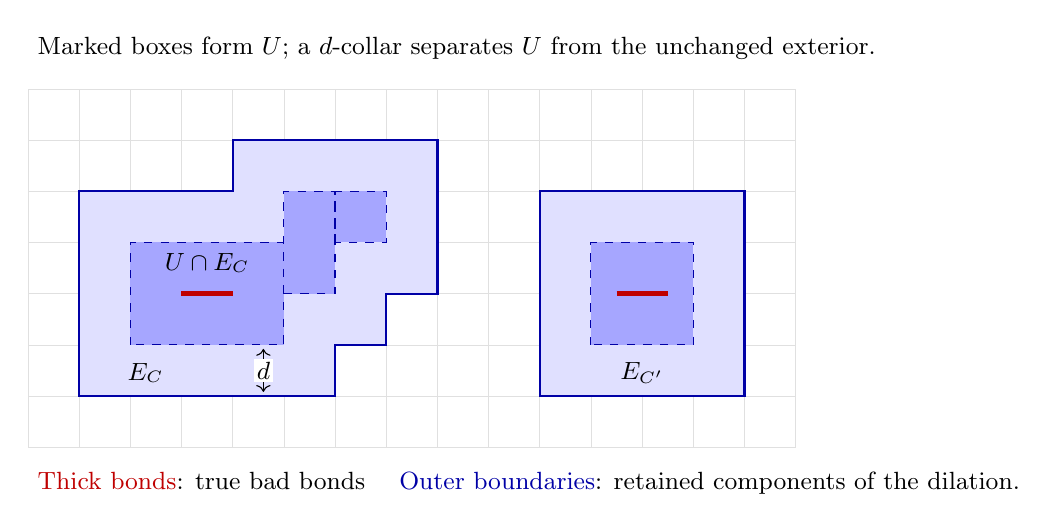
\begin{tikzpicture}[x=0.65cm,y=0.65cm,font=\small]
  \draw[step=1,black!12,very thin] (0,0) grid (15,7);
  \fill[blue!12] (1,1) -- (6,1) -- (6,2) -- (7,2) -- (7,3) -- (8,3) -- (8,6)
      -- (4,6) -- (4,5) -- (1,5) -- cycle;
  \draw[blue!65!black,thick] (1,1) -- (6,1) -- (6,2) -- (7,2) -- (7,3) -- (8,3)
      -- (8,6) -- (4,6) -- (4,5) -- (1,5) -- cycle;
  \fill[blue!35] (2,2) rectangle (5,4);
  \fill[blue!35] (5,3) rectangle (6,5);
  \fill[blue!35] (6,4) rectangle (7,5);
  \draw[blue!65!black,dashed] (2,2) rectangle (5,4);
  \draw[blue!65!black,dashed] (5,3) rectangle (6,5);
  \draw[blue!65!black,dashed] (6,4) rectangle (7,5);
  \fill[blue!12] (10,1) rectangle (14,5);
  \draw[blue!65!black,thick] (10,1) rectangle (14,5);
  \fill[blue!35] (11,2) rectangle (13,4);
  \draw[blue!65!black,dashed] (11,2) rectangle (13,4);
  \draw[red!75!black,line width=2pt] (3,3) -- (4,3);
  \draw[red!75!black,line width=2pt] (11.5,3) -- (12.5,3);
  \node at (2.3,1.45) {$E_C$};
  \node at (12,1.45) {$E_{C'}$};
  \node at (3.5,3.6) {$U\cap E_C$};
  \draw[<->] (4.6,1.08) -- (4.6,1.92);
  \node[fill=white,inner sep=1pt] at (4.6,1.5) {$d$};
  \node[anchor=west,align=left] at (0,7.8)
      {Marked boxes form $U$; a $d$-collar separates $U$ from the unchanged exterior.};
  \node[anchor=west] at (0,-0.7)
      {\textcolor{red!75!black}{Thick bonds}: true bad bonds \quad
       \textcolor{blue!65!black}{Outer boundaries}: retained components of the dilation.};
\end{tikzpicture}
\caption{Schematic editable regions. Each dark region is a union of
marked boxes, and each light region is the complete connected component
of its $d$-dilation. The replacement uses all sites of a selected light
region. Its outer collar lies outside $U$, so it joins the unchanged
configuration without creating a bad bond. Distinct retained components
have nonadjacent sites. The drawing suppresses lattice boundary
conventions and is not to scale.}
\label{fig:editable}
\end{figure}

\FloatBarrier

\begin{lemma}[Replacement and its energy bounds]
\label{lem:editable-regions}
The constants $\varepsilon$ and $C$ can be chosen so that the
following statements hold for all sufficiently large $H$ and
sufficiently large admitted periods.
\begin{enumerate}[label=\textup{(\roman*)}]
\item The unchanged values on $U^c$ have a measurable extension to all
sites in $S^2$ with nearest-neighbor chords at most $C'a$. For each
region $E_C$, independently sampling every spin in a cap of radius
$c't$ about this extension removes all its true bad bonds and creates
none. Any subset of the regions may be replaced in this way. The
conditional sampling density for $n$ replaced sites is at most
$\exp(Cn\log H)$ with respect to product normalized area measure.
\item For a union $E$ of selected regions, let $n=|E|$. There is a set
$I_E$ of rows, consisting of all rows within distance $C'D_1$ of $E$,
which includes every changed kinetic stencil and satisfies
$|I_E|\le Cd^2n$. Its total stencil enlargement is less than $d/2$.
For the original configuration and every sampled replacement $q'$,
\begin{align}
 \sum_{e\in I_E}Y_e(q)&\ge cp^2n/d^2,
 \label{eq:orig-20}\\
 \sum_{e\in I_E}Y_e(q')&\le C_Ld^2p^2n.
 \label{eq:orig-21}
\end{align}
\end{enumerate}
\end{lemma}

\begin{proof}
We first establish the exterior Lipschitz estimate. At a point of
$U^c$, every allowed box containing that point has average gradient
at most $a$. Compare the spin at the point with averages over
successive concentric doubled boxes. The discrete $L^1$ Poincar\'e
inequality, obtained by summing coordinate paths, bounds the change
at scale $R$ by $CR$ times the average gradient on a fixed enlargement.
For two points, stop at the scale of their separation and compare the
two averages through an enclosing box of comparable size. Summing
the geometric scales gives
\[
 |q_x-q_y|\le Ca\,\operatorname{dist}(x,y),\qquad x,y\in U^c.
\]
The radius-one case uses the same coordinate-path estimate. If the
required scale exceeds the allowed box size, the sphere's bounded
diameter proves the estimate once the shortest period is much larger
than $a^{-1}$.

Extend these exterior data componentwise to an $O(a)$-Lipschitz
Euclidean-vector-valued function on the continuous torus, using
distance cones. Within distance $c/a$ of the prescribed data the
extension has norm bounded away from zero; normalization therefore
gives an $S^2$-valued extension there with Lipschitz constant $O(a)$.
Choose a torus mesh of width comparable with $c'/a$, where $c'$ is
sufficiently smaller than $c$. Preserve this extension in every mesh
box meeting the prescribed data. Choose a common arbitrary spin at
all remaining undetermined vertices, and use measurably selected
shortest arcs on the undetermined mesh edges.

Each remaining box now has a boundary map into $S^2$ with uniformly
bounded Lipschitz constant after rescaling. To fill it, cover the
antipodal image curve by $O(1/\tau)$ spherical balls of radius $\tau$.
Their total area is $O(\tau)$, so for a sufficiently small fixed $\tau$
there is a point $p_*$ uniformly separated from the antipodal curve.
If the boundary map in disk coordinates is $g(\theta)$, the normalized
cone
\[
 F(r,\theta)=
 \frac{(1-r)p_*+rg(\theta)}{|(1-r)p_*+rg(\theta)|}
\]
has a uniform Lipschitz bound. A fixed bi-Lipschitz change between a
disk and a square preserves that bound. This is the filling argument
of \Rref{cmp:filling}, with the area of $S^2$ replacing the volume of
$S^3$. Adjacent fillings agree on their already chosen edges. Fixed
ordered nets for $p_*$ and measurable arc choices make the construction
measurable. The same construction works if there are no exterior data.
Rescaling gives the claimed $C'a$ bound.

Choose $\varepsilon$ so that this bound is a sufficiently small
fraction of $t$. Choose the sampling cap radius $c't$ smaller still.
All sampled adjacent spins then have chords below $t$. A boundary
edge of a retained region lies in the collar outside $U$, where the
extension equals the unchanged data; thus crossing edges also remain
below $t$. Every originally true bad bond belongs to a retained
region. Consequently replacing any selected regions removes exactly
their bad-bond inventories. A cap of radius $c't$ on $S^2$ has area
at least $ct^2$, so its normalized sampling density is at most
$C/t^2\le H^C$. Taking products proves the density bound.

For the lower energy estimate, select disjoint generating marked
boxes in each component, in decreasing order of size. Fixed
enlargements of the selected boxes cover all generating boxes.
Dilation by $d$ enlarges the area of a unit or larger box by at most
$Cd^2$. The total selected area in $E_C$ is therefore at least
$c|E_C|/d^2$. On each selected box the average of $f$ exceeds $a$.
If this average is supplied mainly by chords greater than $t$, the
positive linear branch of $S_t$ gives an energy lower bound
$cHa^2$ times the box area. Otherwise Cauchy--Schwarz in the quadratic
branch gives the same lower bound. Bonds incident to disjoint selected
boxes are counted at most a bounded number of times. Since
$Ha^2=\varepsilon^2p^2$, summation proves
Equation~\eqref{eq:orig-20}.

Choose the fixed multiple in $d=CD_1$ after the stencil constants, so
that all stencils read by rows of $I_E$ stay within a $d/2$ enlargement
of $E$. On the replaced sites all chords are below $t$. Any
unselected component of the full dilated construction has its
original marked part at distance at least $d$ from $E$; elsewhere
the unchanged chords are bounded by the exterior estimate. Thus
every chord read by these rows is at most $t$. Uniform summability of
the row weights gives $Y_e(q')\le C_LHt^2=C_Lp^2$.
The support count $|I_E|\le Cd^2n$ proves
Equation~\eqref{eq:orig-21}.
\end{proof}

The lower bound is proportional to the number of replaced sites,
with only the polylogarithmic loss $d^2$. This is what allows an
integrated estimate uniform in the total volume. Fix $B_T$ in
Lemma~\ref{lem:row-exponential-moment} so large that
\begin{equation}
 (1-\theta)C_Ld^2<\frac{c}{4d^2},
 \label{eq:comparison-theta-choice}
\end{equation}
with the constants of Lemma~\ref{lem:editable-regions}. Next take
$P_0$ sufficiently large that
\begin{equation}
 p^2/d^2\gg d^2B_T^2\log H+\log H+1.
 \label{eq:comparison-p-choice}
\end{equation}
All powers on the right were fixed independently of $P_0$. These
requirements can therefore be included among the finite choices
before taking $H$ large.

\subsection{Exact covering identities and integration}

We now keep the geometry of the original configuration fixed while
removing selected inventories. This distinction is important: no
modified configuration is reclustered.

Let $\mathcal I$ be the family of retained regions of a configuration
$q$, and let $D_C$ be the original true bad bonds assigned to $E_C$.
Choose filled values at every region as in
Lemma~\ref{lem:editable-regions}. For $I\subset\mathcal I$, let $q(I)$
be the configuration in which precisely the regions outside $I$ have
been replaced. Then
\begin{equation}
 D(q(I))=\bigsqcup_{C\in I}D_C.
 \label{eq:comparison-inventory-edit}
\end{equation}
Write $\Xi(I)=\Xi(q(I))$; these are complete positive sums.

At a fixed active set $I$, join two labels of a full covering family
if their supports meet the same active region. Call a connected group
a macrolabel $U$. Its enlarged support and weight are
\[
 S_U=\bigcup_{\lambda\in U}P_\lambda
 \ \cup\!
 \bigcup_{\substack{C\in I:\ E_C\cap P_\lambda\ne\varnothing\\
                                  \text{for some }\lambda\in U}}E_C,
 \qquad
 w(U;q(I))=\prod_{\lambda\in U}k_\lambda(q(I)).
\]
All labels supplying the inventory of a touched region belong to the
same group, so each macrolabel covers every active region it meets
in full. Distinct macrolabels have disjoint enlarged supports.
Conversely, compatible macrolabels covering the active inventories
recover a full original covering family.

If a site set $S$ is disjoint from the active regions, denote by
$\Xi(I;S)$ the complete-inventory sum restricted to macrolabels
whose enlarged supports avoid $S$. This restricted sum may be signed.
For a selected compatible macrolabel family $\mathcal A$, let
$S_{\mathcal A}$ be its combined support and $B_{\mathcal A}$ the
active regions it covers. The exact identities from
\Rref{cmp:background-identity}, \Rref{cmp:IE}, and
\Rref{cmp:difference-identity} become
\begin{align}
 \Xi(I;S)
 &=\sum_{\substack{\mathcal A\ \mathrm{compatible}\\
          S_U\cap S\ne\varnothing\ (U\in\mathcal A)}}
 (-1)^{|\mathcal A|}
 \prod_{U\in\mathcal A}w(U;q(I))\,
 \Xi(I\setminus B_{\mathcal A};S_{\mathcal A}),
 \label{eq:comparison-inclusion-exclusion}\\
 \widetilde\Xi(I)-\Xi(I)
 &=\sum_{\substack{\mathcal A\ \mathrm{compatible}\\
                              \mathcal A\ne\varnothing}}
 \prod_{U\in\mathcal A}
       [\widetilde w(U;q(I))-w(U;q(I))]\,
 \Xi(I\setminus B_{\mathcal A};S_{\mathcal A}).
 \label{eq:comparison-difference-identity}
\end{align}
Here and below macrolabels in a displayed sum satisfy the inventory
conditions just described.

To verify the identities, first select a compatible family. Every
remaining support avoids $S_{\mathcal A}$ and hence every changed
site. Its values and all eligibility indicators are unchanged by
removing $B_{\mathcal A}$. Its inventory loses exactly the removed
inventories in Equation~\eqref{eq:comparison-inventory-edit}. This
gives the background sum
$\Xi(I\setminus B_{\mathcal A};S_{\mathcal A})$.
Expand the indicator of avoiding $S$ as a product of
$1-\mathbf1_{\{S_U\cap S\ne\varnothing\}}$ to obtain the first
identity. Expand $\widetilde w=w+(\widetilde w-w)$ in a full family
and subtract the all-$w$ term to obtain the second. With finite label
lists these are finite algebraic identities. A full family contains
at most $|D(q(I))|$ labels, and the absolute activity bounds give
convergence for countable lists, so the identities pass to that
limit before any division is performed.

Starting with Equation~\eqref{eq:comparison-difference-identity},
iterate Equation~\eqref{eq:comparison-inclusion-exclusion} until
each term ends in a complete base sum $\Xi(q')$. Every nonempty
generation consumes an active region, so this recursion terminates.
Fix an ordering of the common label list. Take absolute values and
telescope each initial macrolabel difference in this order:
\begin{equation}
 |\widetilde w(U)-w(U)|
 \le\sum_{\lambda\in U}d_\lambda
             \prod_{\kappa\in U\setminus\{\lambda\}}p_\kappa.
 \label{eq:comparison-marked-product}
\end{equation}
Thus each initial macrolabel has one marked original label, carrying
$d_\lambda$; the other labels carry $p_\lambda$. The final complete
$\Xi(q')$ is positive.

We record explicitly the gain after integrating such a term. A term
will be encoded below by its original labels and the exact site sets
of its consumed regions. Fix these sets, let their union be $E$, and
put $n=|E|$. Let $\mathcal Q$ be the measurable set of original
configurations whose region construction and original inventories admit
this encoded term. Label lists include zero-valued labels: every
spin-dependent eligibility test remains in the evaluated weight. Thus
$\mathcal Q$ is defined before sampling, even when a later evaluated
weight vanishes for some filled values. Average over the sampled
filled values; only consumed regions need to be sampled. Then
\begin{equation}
 \frac1Z\int_{\mathcal Q} e^{X(q)}
           \E_{\mathrm{fill}\mid q}[\Xi(q')]\,\dd q
 \le e^{-c'p^2n/d^2}.
 \label{eq:orig-22}
\end{equation}
Indeed Equations~\eqref{eq:orig-17} and~\eqref{eq:orig-20} imply
\[
 X(q)-X(q')\le C_Ln-cp^2n/d^2+\sum_{e\in I_E}Y_e(q').
\]
By Equation~\eqref{eq:orig-21} and the choice
\eqref{eq:comparison-theta-choice}, replacing the last coefficient
one by $\theta$ costs at most $cp^2n/(4d^2)$.

There is no change-of-variables invertibility assumption here.
Write $q=(q_E,q_{E^c})$ and let
$h(q'_E\mid q_E,q_{E^c})$ be the conditional fill density. Its
uniform bound is $e^{Cn\log H}$. After using that bound, positivity
of $\Xi(q')$ allows the restrictions defining $\mathcal Q$ to be
dropped. Integration over the original $q_E$ contributes at most
one, since it uses product probability measure. The remaining
integral over $(q'_E,q_{E^c})$ is bounded by
\[
 \exp\left(C_Ln+Cn\log H-\frac{3cp^2n}{4d^2}\right)
 \E_\mu\exp\left(\theta\sum_{e\in I_E}Y_e\right).
\]
Equation~\eqref{eq:orig-19}, $|I_E|\le Cd^2n$, and
Equation~\eqref{eq:comparison-p-choice} prove
Equation~\eqref{eq:orig-22}. This is the only integration estimate
needed in the covering recursion; no restricted signed sum appears
in a denominator.

\subsection{Summing the forests}

We complete the proof of Proposition~\ref{prop:integrated-comparison}
by explaining the counting in \Rref{cmp:forest} for these regions.
Inside each macrolabel choose a spanning tree on its original label
nodes and the active-region nodes it meets. Make the choice
deterministically using a fixed ordering. Join each later macrolabel,
again deterministically, to one preceding-generation macrolabel whose
support it meets. Choose a deterministic intersecting pair of their
underlying gas or region supports as the endpoints of this edge. Use
two edge colors to distinguish edges internal
to a macrolabel from edges joining generations, and root each tree
at the marked label of its initial macrolabel.

No region node is repeated: a region is consumed on first appearance.
No original label is repeated either. Its inventory is fixed and
nonempty, and the regions containing it have already been removed
after its first appearance. It cannot be eligible in a subsequent
generation. Within a generation the supports are disjoint.

This forest retains the entire term. Contracting internal edges
recovers the macrolabels; depths in the contracted rooted forest
recover generations; marked roots recover the telescoping choices.
The exact region site sets recover the consumed active sets and
therefore every evaluation configuration. Thus distinct terms do
not acquire the same forest. For a fixed original configuration the
unconsumed geometry and inventories are already determined; there
is no further multiplicity to count.

After integration, Equation~\eqref{eq:orig-22} assigns an edit node
$E_C$ the weight
\[
 w(E_C)=e^{-c'p^2|E_C|/d^2}.
\]
Since the consumed sets are disjoint, their product is exactly the
weight for their union. We may now enlarge the possible geometries
to all connected site animals. On a bounded-degree lattice the number
of animals of size $n$ containing a fixed site is at most $C^n$;
the same bound follows by a spanning-tree traversal on a torus.
Consequently, with $R=C_L\mathfrak m_0^2$ large enough that
$|P_\lambda|\le Rs_\lambda$,
\[
 \sup_x\sum_{E_C:x\in E_C}w(E_C)e^{2|E_C|}
 \le\sum_{n\ge1}C^ne^{-(c'p^2/d^2-2)n}
 <\frac1{16R}
\]
for sufficiently large $H$. The activity cap likewise gives
\[
 \sup_x\sum_{\lambda:x\in P_\lambda}
                    p_\lambda e^{2s_\lambda}<\frac1{16R}.
\]
Indeed $A=64\ge2$ and $Rw_0\to0$, even after multiplying the cap by
any fixed constant, by Equation~\eqref{eq:setup-covering-norm}.
Give a gas node size $s_\lambda$ and an edit node size $|E_C|$.
Every node of size $b$ has support at most $Rb$. Summing over an
intersection site and the two edge colors bounds the one-child sum,
with an exponential allowance for descendants, by $b/4$.

More explicitly, induction on maximum tree depth bounds the total
descendant weight below a root of size $b$ by $e^b$. For the induction
step, a child of size $a$ contributes at most its weight times $e^a$.
The sum over unordered distinct children is bounded by the
exponential of the one-child sum, because ordered $r$-tuples with
factor $1/r!$ only enlarge it after distinctness is dropped. Hence
the descendant sum is at most $e^{b/4}\le e^b$. Monotonicity of the
positive majorants allows arbitrary depth.

A marked gas root therefore costs at most
$d_\lambda e^{s_\lambda}\le d_\lambda e^{2s_\lambda}$.
Actual forest components have distinct marked roots. Dropping all
disjointness conditions between their descendant trees and summing
unordered nonempty root sets gives
\[
 \sum_{r\ge1}\frac1{r!}
 \left(\sum_\lambda d_\lambda e^{2s_\lambda}\right)^r.
\]
This is the right-hand side of Equation~\eqref{eq:orig-16}, proving
Proposition~\ref{prop:integrated-comparison}.

\subsection{Partition functions and ordinary alignment}

Apply Proposition~\ref{prop:integrated-comparison} to the two endpoint
gases in Equation~\eqref{eq:orig-15}. Summing their support-hit bound
over sites gives
\[
 \sum_\lambda d_\lambda e^{2s_\lambda}\le D_Hv\delta_K.
\]
The exponent comparison in that equation then shows that the ratio
of the scalar-stripped partition functions tends to one whenever
$v\delta_K\to0$. For example, with $\varepsilon_K=D_Hv\delta_K$,
\[
 \left|\frac{\int e^{X_1}\Xi_2}{\int e^{X_1}\Xi_1}-1\right|
 \le e^{\varepsilon_K}-1,
 \qquad
 e^{-\varepsilon_K}\le e^{X_2-X_1}\le e^{\varepsilon_K}.
\]
For small $\varepsilon_K$ these inequalities bound the logarithm of
the partition-function ratio by $C\varepsilon_K$. The constants
depend on the fixed $H$, but not on depth or period. The same
integrated estimate will also be used when activity differences
are localized at specified source sites, in which case their sum
does not carry a factor $v$.

We also need a local consequence of reflection positivity.

\begin{corollary}[Terminal alignment]
\label{cor:terminal-alignment}
On every standard terminal axis torus considered in this section,
for each fixed $C>0$ there is $c>0$ such that every bond satisfies
\begin{equation}
 \mu\{|q_x-q_y|>t/C\}\le e^{-cHt^2}.
 \label{eq:orig-23}
\end{equation}
The constants are uniform in the cutoff depth and the admitted periods.
\end{corollary}

\begin{proof}
Choose a translated $2$-by-$2$ tile containing the specified bond and
disseminate its event by tile reflections. The periods are divisible
by $2B_T$, hence by $4$, so these tiles have even counts in both
directions. A fixed positive fraction of all bonds then have chord
greater than $t/C$.
The direct kinetic energy on that event is at least $cHt^2v$.
Equations~\eqref{eq:orig-17} and~\eqref{eq:orig-18} bound its
probability by
\[
 \exp[-v(cHt^2-C_L-C_L\log H)]\le e^{-c'vHt^2}.
\]
The chessboard inequality gives the single-event bound after taking
the corresponding tile root. This is the argument of
\Rref{cmp:rarity}, whose hypotheses have now all been checked for
the $S^2$ endpoint law. No such estimate is used in oblique periods.
\end{proof}

\section{Trace estimates uniform in the cutoff}
\label{sec:trace}

The endpoint comparison now produces a box of fixed physical size in
which the excited transfer trace is small at every sufficiently fine
cutoff.  Positivity then propagates this information to arbitrarily
large boxes.  This section proves both consequences needed below: a
uniform comparison between finite tori and the plane, and exponential
decorrelation at a fixed positive rate in physical units.  The transfer
argument follows \cite{OpenAI-O4}, \Rref{sec:finite-volume}; we give its
proof, including the rectangular and sheared periods used here.

Write $Z_\beta(n,w)$ for the nearest-neighbour partition function on the
torus with time period $n$ and spatial period $w$, using normalized area
measure at every spin.  All geometric periods below, including the
auxiliary half-periods, are at least four.  Define
\begin{equation}
 \Delta_\beta(n,w)
   =4\log Z_\beta(n,w)-\log Z_\beta(2n,2w).
 \label{eq:trace-doubling-definition}
\end{equation}
The coefficients cancel every contribution to $\log Z$ proportional to
the area.  In particular, the bulk scalars extracted by the exact
renormalization do not contribute to $\Delta_\beta$.

\subsection{A fixed physical box}

The gain in the preliminary length estimate and the contraction of
endpoint discrepancies have complementary roles.  The former makes a
reference box large enough to mix; the latter allows that box to be
compared with every finer cutoff.

\begin{proposition}[A uniform reference-box test]
\label{prop:trace-small-box}
Let $\mathcal U\subset(\mathbb Q_{>0})^2$ be finite.  Assume the
preliminary estimate of Section~\ref{sec:preliminary}, the shooting
asymptotics \eqref{eq:orig-12}, the endpoint discrepancy estimate
\eqref{eq:orig-15}, and the integrated comparison
\eqref{eq:orig-16}.  With the contraction slack $\upsilon>0$ chosen
sufficiently small, there exist an integer $K_0$ and a positive integer
$M_0$, independent of $N$, such that, for every $N\ge K_0$ and every
$(u_1,u_2)\in\mathcal U$,
\begin{equation}
 \Delta_{\beta_N}(n,w)\le 2^{-10},
 \qquad (n,w)=(u_1,u_2)M_0L^N.
 \label{eq:orig-24}
\end{equation}
The number $M_0$ may be required to exceed any prescribed fixed constant
and to be divisible by any prescribed fixed integer.  In particular,
all periods and tile counts needed in
Section~\ref{sec:comparison} may be taken to be even integers.
\end{proposition}

\begin{proof}
Let $\eta>0$ be the gain in \eqref{eq:orig-1}.  Choose
\[
 0<\frac{\upsilon}{2}<\chi<\min\left\{1,\frac{\eta}{2\pi}\right\}.
\]
Take $m_K$ to be a fixed common integer multiple of a dyadic integer,
rounded so that
\begin{equation}
 \log_L m_K=(1-\chi)K+O(1),\qquad
 2(1-\chi)<2-\upsilon,\qquad
 2-\chi>\frac{4\pi-\eta}{2\pi}.
 \label{eq:trace-scale-choice}
\end{equation}
The fixed multiple clears the denominators in $\mathcal U$ and imposes
the divisibility conditions of the proposition.

At depth $K$, Equation~\eqref{eq:orig-12} and
$\gamma=(\log L)/(2\pi)$ give
\[
 X(\beta_K)
   \le C_H K^{C_H} L^{(2-\eta/(2\pi))K}.
\]
The shorter side of a reference rectangle
$(u_1,u_2)m_KL^K$ is a fixed positive multiple of
$L^{(2-\chi)K}$.  Its ratio to $X(\beta_K)$ therefore grows
exponentially in $K$.  The preliminary doubling estimate consequently
implies
\[
 \max_{(u_1,u_2)\in\mathcal U}
 \left|\Delta_{\beta_K}(u_1m_KL^K,u_2m_KL^K)\right|
     \longrightarrow0.
\]
Indeed its exponentially decaying factor dominates every polynomial
prefactor in the microscopic periods and in $\beta_K$.

For $N\ge K$, run both cutoffs to the same terminal rectangle with
periods $(u_1,u_2)m_K$.  Its volume is
$v=u_1u_2m_K^2$.  Equations~\eqref{eq:orig-15} and
\eqref{eq:orig-16}, with the exponent discrepancy included, imply
that the logarithms of the two scalar-stripped partition functions
differ by at most $C_Hv\delta_K$ whenever $v\delta_K$ is sufficiently
small.  The estimate is uniform in $N\ge K$.  Apply it also to the
doubled rectangle, whose terminal volume is $4v$.  Cancellation of the
bulk scalars gives
\begin{align*}
 &\left|\Delta_{\beta_N}(u_1m_KL^N,u_2m_KL^N)
       -\Delta_{\beta_K}(u_1m_KL^K,u_2m_KL^K)\right|\\
 &\hspace{35mm}\le C_Hm_K^2\delta_K
       \longrightarrow0,
\end{align*}
because $\delta_K=L^{-(2-\upsilon)K}$ and
$2(1-\chi)<2-\upsilon$.  Constants may depend on the finite list
$\mathcal U$, but not on $N$ or $K$.  Choose one sufficiently large
$K_0$ and put $M_0=m_{K_0}$.
\end{proof}

\subsection{Positive transfer and repeated doubling}

We next isolate the spectral content of the partition-function test.
For a fixed spatial circumference $w$, a time slice is
$s=(s_1,\ldots,s_w)\in(S^2)^w$.  Put
$V_w(s)=\sum_{i=1}^w s_i\cdot s_{i+1}$, with periodic indices.
On $L^2((S^2)^w)$ define the transfer operator $K_w$ by the kernel
\begin{equation}
 K_w(s,s')=
 \exp\left\{\frac\beta2V_w(s)
       +\beta\sum_{i=1}^w s_i\cdot s_i'
       +\frac\beta2V_w(s')\right\}.
 \label{eq:trace-kernel}
\end{equation}
The coupling $\beta\ge0$ is fixed in this subsection and suppressed
from the notation.  All Hilbert spaces use product probability measure.

The kernel is continuous, symmetric, and strictly positive.  Its
positive semidefiniteness is a separate property: the expansion
\[
 e^{\beta s\cdot s'}
   =\sum_{j=0}^{\infty}\frac{\beta^j}{j!}
       \inner{s^{\otimes j}}{(s')^{\otimes j}}
\]
is a sum of positive semidefinite kernels.  Tensor products over sites
and multiplication on both sides by $e^{\beta V_w/2}$ preserve that
property.  The sum of their diagonal integrals is finite, so the same
expansion proves that $K_w$ is trace class.  Strict positivity of the
kernel gives a simple largest eigenvalue with a strictly positive
normalized eigenfunction $\Omega_w$.  Write
\[
 \lambda_1(w)>\lambda_2(w)\ge\lambda_3(w)\ge\cdots\ge0,
 \qquad
 Z_\beta(n,w)=\Tr K_w^n=\sum_i\lambda_i(w)^n.
\]
If only one eigenvalue is nonzero, all subsequent statements are read
with $\lambda_2=0$.  These observations also verify directly the
transfer hypotheses of \Rref{prop:criterion} for $S^2$ spins.

Define the two one-direction defects
\begin{align}
 p(n,w)&=2\log Z_\beta(n,w)-\log Z_\beta(2n,w),\notag\\
 q(n,w)&=2\log Z_\beta(n,w)-\log Z_\beta(n,2w).
 \label{eq:trace-one-direction}
\end{align}
Both are nonnegative, using transfer positivity in the respective
coordinate directions.  The excited trace relative to the largest
eigenvalue is
\[
 s_n(w)=\sum_{i\ge2}
       \left(\frac{\lambda_i(w)}{\lambda_1(w)}\right)^n.
\]

\begin{lemma}[Concentration of the transfer trace]
\label{lem:trace-concentration}
For every integer $n\ge4$,
$s_n(w)\le e^{p(n,w)}-1$.  If $p(n,w)\le1/4$, then
\begin{equation}
 \left(\frac{\lambda_2(w)}{\lambda_1(w)}\right)^n
       \le2p(n,w),\qquad
 p(2n,w)\le4p(n,w)^2.
 \label{eq:trace-squaring}
\end{equation}
The corresponding conclusions hold for $q$ with the coordinate
directions interchanged.
\end{lemma}

\begin{proof}
Set $t_i=\lambda_i(w)^n/\sum_j\lambda_j(w)^n$.  Then
\[
 e^{-p(n,w)}=\sum_i t_i^2\le t_1=(1+s_n(w))^{-1}.
\]
This gives the first assertion and, when $p\le1/4$, the bound
$s_n\le pe^p\le2p$.  Moreover $s_{2n}\le s_n^2$, and cancellation
of the largest eigenvalue yields
\[
 p(2n,w)=2\log(1+s_{2n})-\log(1+s_{4n})
     \le2s_n^2\le2p(n,w)^2e^{2p(n,w)}
     \le4p(n,w)^2.
\]
This is the proof of \Rref{lem:squaring}, with no dependence on the
dimension of the spin sphere.
\end{proof}

Small excited weight at one circumference alone would leave open the
appearance of low-energy states at larger circumferences.  The second
direction in $\Delta$ supplies the missing control.  Direct substitution
in \eqref{eq:trace-one-direction} gives
\begin{align}
 \Delta_\beta(n,w)
   &=2p(n,w)+q(2n,w)
     =2q(n,w)+p(n,2w),\notag\\
 p(n,2w)&=2p(n,w)-2q(n,w)+q(2n,w).
 \label{eq:trace-rectangle-identities}
\end{align}
In particular, $\Delta_\beta(n,w)\ge0$.

\begin{proposition}[Rectangular doubling criterion]
\label{prop:trace-doubling}
Let $\beta\ge0$ and let $n,w\ge4$ be integers.  If
$\Delta_\beta(n,w)\le2^{-10}$, then, for every $k\ge0$,
\begin{equation}
 \Delta_\beta(2^kn,2^kw)\le64^{-1}2^{-2^k}.
 \label{eq:orig-25}
\end{equation}
For a square with $n=w$, the transfer operators at circumferences
$2^kn$ also satisfy
\begin{equation}
 \frac{\lambda_2(2^kn)}{\lambda_1(2^kn)}
       \le e^{-(\log2)/n}.
 \label{eq:trace-width-gap}
\end{equation}
\end{proposition}

\begin{proof}
Write $\Delta=\Delta_\beta(n,w)$.  The two expressions in
\eqref{eq:trace-rectangle-identities} imply
$q(2n,w)\le\Delta$ and $p(n,2w)\le\Delta$.  Consequently
\[
 p(2n,2w)\le4\Delta^2.
\]
The interchanged rectangle identity then gives
\[
 q(4n,w)=2q(2n,w)-2p(2n,w)+p(2n,2w)
       \le2\Delta+4\Delta^2\le3\Delta.
\]
Squaring in the spatial direction gives
$q(4n,2w)\le36\Delta^2$, and hence
\[
 \Delta_\beta(2n,2w)
   =2p(2n,2w)+q(4n,2w)
   \le44\Delta^2\le64\Delta^2.
\]
Every application of Lemma~\ref{lem:trace-concentration} is permitted
by $3\cdot2^{-10}<1/4$, and the smallness condition is preserved.
Iteration yields
\[
 \Delta_\beta(2^kn,2^kw)
       \le64^{-1}(64\cdot2^{-10})^{2^k}
       \le64^{-1}2^{-2^k}.
\]
For a square, put $n_k=2^kn$.  The same lemma gives
\[
 \left(\frac{\lambda_2(n_k)}{\lambda_1(n_k)}\right)^{n_k}
       \le2p(n_k,n_k)\le\Delta_\beta(n_k,n_k).
\]
Taking the $n_k$-th root proves
\eqref{eq:trace-width-gap}.  Thus the square proof of
\Rref{prop:criterion} also proves the asserted rectangular recursion;
no equality of the original periods entered that recursion.
\end{proof}

\subsection{Local insertions and the volume limit}

To use the trace bound for correlations, one needs control of an
insertion that may occupy an entire time slab.  The following estimate
has no cost depending on the number of spins read by the insertion.
Let $F$ be a bounded local observable supported in a slab of $r$
transfer steps.  The kernel $K_{w,F}$ obtained by inserting $F$ in that
slab satisfies
\[
 |K_{w,F}(s,s')|\le\norm{F}_\infty K_w^r(s,s').
\]
With $T_w=K_w/\lambda_1(w)$ and
$A_F=K_{w,F}/\lambda_1(w)^r$, positivity of $K_w^r$ implies
$\norm{A_F}\le\norm{F}_\infty$: apply the pointwise inequality to
$|f|$ and use $\norm{T_w^r}=1$.  When $r=0$, $A_F$ is multiplication
by $F$.  The infinite-time cylinder expectation is therefore
\[
 \omega_w(F)=\inner{\Omega_w}{A_F\Omega_w}.
\]

Let $P_w$ be the orthogonal projection onto $\Omega_w$.  Since
$T_w-P_w$ is positive semidefinite,
$\Tr(T_w^j-P_w)=s_j(w)$.  For $r\le n/2$, splitting off $P_w$ in
\[
 \mu_{\beta;n,w}(F)
    =\frac{\Tr(A_FT_w^{n-r})}{\Tr T_w^n}
\]
gives
\begin{equation}
 |\mu_{\beta;n,w}(F)-\omega_w(F)|
      \le2\norm{F}_\infty s_{n/2}(w),
 \label{eq:trace-torus-cylinder}
\end{equation}
whenever $n$ is even.  Here $\mu_{\beta;n,w}$ denotes the probability
law on the rectangular torus.  The same calculation applies after
interchanging space and time.

We state the resulting volume comparison with the auxiliary aspect
ratios specified explicitly.  This makes the finite amount of
information required from Proposition~\ref{prop:trace-small-box}
independent of all later limits.  For complex observables the covariance
is sesquilinear:
$\Cov_\omega(F,G)=\omega(\overline F G)
 -\omega(\overline F)\omega(G)$.

\begin{theorem}[Uniform volume comparison and slab decorrelation]
\label{thm:trace-uniform}
Let $\mathcal A\subset(\mathbb Q_{>0})^2$ be a finite list containing
$(1,1)$ and $(1,25)$, and put
\[
 \mathcal U=\mathcal A
    \cup\{(u_1/2,u_2):(u_1,u_2)\in\mathcal A\}
    \cup\{(2u_1,u_2/2):(u_1,u_2)\in\mathcal A\}.
\]
Choose $K_0,M_0$ by Proposition~\ref{prop:trace-small-box} for
$\mathcal U$, with all displayed periods even and at least four.  Let
$\omega_{\beta_N}$ be the periodic infinite-plane state supplied by
Section~\ref{sec:preliminary}.  There are constants $C,c>0$, independent
of $N\ge K_0$ and $k\ge0$, with the following properties.

For $(u_1,u_2)\in\mathcal A$, set
$(n,w)=(u_1,u_2)2^kM_0L^N$.  If a bounded local observable $F$ can be
placed in a rectangle of time extent at most $n/2$ and spatial extent
at most $w/2$, then
\begin{equation}
 |\mu_{\beta_N;n,w}(F)-\omega_{\beta_N}(F)|
       \le C\norm{F}_\infty e^{-c2^k}.
 \label{eq:trace-uniform-volume}
\end{equation}
The same estimate holds for a torus obtained by closing time with any
integer spatial translation, provided the support has a lift of time
extent at most $n/2$ and spatial extent at most $w/2$.

For bounded local observables $F,G$ on the plane whose supporting time
slabs are separated by $d\ge0$ transfer edges,
\begin{equation}
 |\Cov_{\omega_{\beta_N}}(F,G)|
    \le\norm{F}_\infty\norm{G}_\infty
       e^{-c d/(M_0L^N)}.
 \label{eq:orig-26}
\end{equation}
The constant in this last estimate may be taken to be $c=\log2$.
\end{theorem}

\begin{proof}
First compare $(n,w)$ with $(2n,w)$.  Both torus expectations are
within $2\norm{F}_\infty s_{n/2}(w)$ of the cylinder expectation at
circumference $w$, by \eqref{eq:trace-torus-cylinder}.  The auxiliary
aspect $(u_1/2,u_2)$ and Proposition~\ref{prop:trace-doubling} give
\[
 s_{n/2}(w)
    \le e^{p(n/2,w)}-1
    \le e^{\Delta_{\beta_N}(n/2,w)}-1
    \le C e^{-c2^k}.
\]
Next compare $(2n,w)$ with $(2n,2w)$, applying the same argument in
the spatial direction.  The needed excited trace has running length
$w/2$ and transverse circumference $2n$; it is bounded using
$q(2n,w/2)\le\Delta_{\beta_N}(2n,w/2)$ and the auxiliary aspect
$(2u_1,u_2/2)$.  Thus consecutive simultaneous doublings differ by
at most $C\norm{F}_\infty e^{-c2^k}$.  Sum this estimate over all
subsequent doublings.  At fixed $N$, the limit is the periodic
infinite-plane state from Section~\ref{sec:preliminary}, giving
\eqref{eq:trace-uniform-volume}.

For completeness, this identification also holds for bounded
measurable local observables.  At fixed cutoff and fixed finite
support, nearest-neighbour conditional densities give a uniform upper
bound, independent of the enclosing torus, for the marginal density
relative to product area measure.  Approximation in that reference
measure extends the identity from continuous to bounded measurable
observables.  The direct transfer estimates above already have the
same supremum-norm bound for such observables.

Now close time with a spatial shift $s\in\mathbb Z/w\mathbb Z$.
Let $U_s$ be its unitary action on $L^2((S^2)^w)$.  Translation
invariance gives $U_sT_w=T_wU_s$.  Simplicity and positivity of the
ground state give $U_s\Omega_w=\Omega_w$.  Choosing the closing seam
outside the supporting slab, the normalized partition function and
the inserted numerator are
\[
 \Tr(T_w^nU_s),\qquad \Tr(A_FT_w^{n-r}U_s).
\]
Their ground-state contributions are $1$ and $\omega_w(F)$,
respectively, and their remaining contributions have absolute values
at most $s_n(w)$ and $\norm{F}_\infty s_{n-r}(w)$.  The half-period
bound just proved ensures $s_n(w)<1/2$.  Consequently
\[
 |\mu_{\beta_N;n,w}^{(s)}(F)-\omega_w(F)|
     \le4\norm{F}_\infty s_{n/2}(w).
\]
Comparison with the unshifted torus, followed by
\eqref{eq:trace-uniform-volume}, proves the assertion for shifted
closing conditions, uniformly in $s$.

Finally put $n_0=M_0L^N$.  The square reference-box test and
\eqref{eq:trace-width-gap} imply, at every circumference
$w=2^kn_0$,
\[
 \norm{T_w^d-P_w}\le e^{-(\log2)d/n_0}.
\]
For two ordered slab insertions on the cylinder,
\[
 \Cov_{\omega_w}(F,G)
   =\inner{\Omega_w}{A_{\overline F}(T_w^d-P_w)A_G\Omega_w}.
\]
The insertion norm estimate therefore proves
\eqref{eq:orig-26} on these cylinders with $c=\log2$.
Equation~\eqref{eq:trace-torus-cylinder}, using the half-period
trace bound, identifies their local limits with the square-torus
limit.  Passage to that limit proves the assertion on the plane.
\end{proof}

\subsection{A uniform physical gap}

The slab estimate controls the whole transfer spectrum, because it
applies to all bounded local observables.  Its spectral consequence is
therefore stronger than a bound on the spin two-point function alone.

\begin{corollary}[A uniform physical gap]
\label{cor:trace-physical-gap}
For $N\ge K_0$, let $\mathcal T_N$ be the one-step transfer contraction
in the reflection-positive Hilbert space of $\omega_{\beta_N}$, and
let $\Omega_N$ be its vacuum vector.  Then
\[
 \spec\bigl(\mathcal T_N|_{\Omega_N^\perp}\bigr)
    \subset\left[0,e^{-(\log2)/(M_0L^N)}\right].
\]
At lattice spacing $a_N=L^{-N}$, the lower energy scale in physical
units is consequently
\begin{equation}
 \frac{1}{a_N}\frac{\log2}{M_0L^N}
       =\frac{\log2}{M_0}>0.
 \label{eq:trace-physical-scale}
\end{equation}
\end{corollary}

\begin{proof}
Link reflection positivity follows from positive semidefiniteness of
the crossing-bond kernel $e^{\beta s\cdot s'}$; site reflection
positivity follows by conditional factorization across the fixed row.
Both pass to the periodic plane limit and make $\mathcal T_N$ a
positive semidefinite self-adjoint contraction.
A centered bounded local observable creates a vector whose transfer
autocorrelation is the covariance of two reflected slabs.
Equation~\eqref{eq:orig-26} bounds this autocorrelation by
$C_\psi e^{-(\log2)j/(M_0L^N)}$, with $C_\psi$ depending on the vector
and its slab thickness.  The spectral measure is positive.  Positive
mass on any interval $[r,1]$ with
$r>e^{-(\log2)/(M_0L^N)}$ would give a lower bound proportional to
$r^j$, contradicting that decay.  Centered bounded local vectors are
dense in the vacuum orthogonal subspace.  Boundedness of spectral
projections therefore gives the asserted exclusion for the whole
subspace, as in \Rref{prop:criterion}.  Dividing the negative logarithm
of a nonzero transfer spectral value by $a_N$ gives the physical
energy bound \eqref{eq:trace-physical-scale}.
\end{proof}

The constants and the physical volume threshold have been fixed before
removing the cutoff.  Continuum convergence is established in
Section~\ref{sec:continuum}; Section~\ref{sec:os} then transfers this
cutoff-independent positive scale to the continuum Hamiltonian.

\subsection{Tilted periods}

The only nonrectangular periods needed in the construction are covered
by the shifted closing condition in Theorem~\ref{thm:trace-uniform}.
Let $M=2^kM_0$.  A square of physical side $5M$ tilted by $O_+$ has
period vectors
\[
 a=M(3,4),\qquad b=M(-4,3)
\]
in the regulator axes, with coordinate pairs in this paragraph written
as $(\mathrm{space},\mathrm{time})$.  The integer change of basis
\[
 3a-4b=(25M,0),\qquad a-b=(7M,M)
\]
has determinant one.  The same torus therefore has spatial
circumference $25M$, time height $M$, and a spatial shift $7M$ upon
closing time.  Dividing by $a_N=L^{-N}$ makes all periods and shifts
integers.  Reflected versions, including $O_-$ in the other regulator
frame, have the same circumference and height, with a possibly
different shift.  A fixed compact physical support has a lift satisfying
both extent bounds for all sufficiently large $k$, uniformly in $N$.
Thus the finite list containing
$(1,25)$ and its auxiliary aspects supplies all the tilted-torus
comparisons needed later.

\section{Exact renormalization of the spin sources}
\label{sec:sources}

The estimates obtained so far concern densities and partition functions.
To construct fields, we must also compare local observables at different
cutoffs.  We do this by carrying independent sources through the exact
block integration.  The coefficient of the linear spin source determines
the field normalization.  The coupling prescription of
Section~\ref{sec:shooting} remains the prescription at zero source.

Throughout this section a step has side factor $l=L$ or $l=L_*=5L$ and
maps layer $j$ to layer $j-1$.  We use the scales and graph norms of
Section~\ref{sec:rg}; in particular $k=8$, and
\[
 R_j:=H_j^{-1/10}.
\]
The estimates in this section require no information about the
infinite-volume state.  They apply in bulk and on every compatible
period admitted in Section~\ref{sec:free}.

\subsection{The source class and the exact step}

At each site $x$ let $z_x=(z_x^1,z_x^2,z_x^3)\in\C^3$ be an independent
variable.  For a power series $F(q;z)=\sum_\alpha F_\alpha(q)z^\alpha$,
where $\alpha$ ranges over finitely supported multi-indices in the
site and component variables, its coefficient norm at radius $r$ is
\[
 [F]_{k,j;r}:=\sum_\alpha r^{|\alpha|}[F_\alpha]_{k,j}.
\]
The same convention applies to supremum and activity norms.  A
coefficient of a regular function is measured on its graph domain;
a covering activity is measured by its supremum.  We omit $r$ when
$r=1$.  Absolute coefficient sums form a product majorant: products
are bounded by coefficient convolution before any integration or
graph summation.  In particular, identifying source variables does
not increase this norm.

We adjoin to a density in the class of Section~\ref{sec:rg} the
exponent
\[
 \sum_x z_x\cdot q_x+\sum_X 1_XG_X(q;z)
\]
and source-dependent covering activities $k^{\mathrm{src}}_\lambda(q;z)$.
Every $G_X$ and $k^{\mathrm{src}}_\lambda$ has positive source degree.
The graph domain of $G_X$, its load $s_X$, and its mask $1_X$ are those
of a regular error.  Its complete support includes every source site
appearing in it.  Covering labels retain their nonempty inventories of
bad bonds and their complete spin and source dependencies.  All masks
test spin chords only; they impose no condition on a source variable.

The source lists satisfy
\begin{equation}
 \sup_o\sum_{X\text{ anchored at }o}e^{As_X}[G_X]_{k,j}
       \le R_j,
 \qquad
 \norm{k^{\mathrm{src}}}_{j,A}\le w_j.
 \label{eq:orig-27}
\end{equation}
We may separate a regular list by degree or by its multiset of source
indices.  Each such record is anchored at one of those indices; in
degree one this is the unique source site.  Bulk and nonwinding
degree-one regular functions vanish when all their spin arguments
are equal.  No such normalization is imposed on winding records,
and no alignment normalization is imposed in higher source degree.
In particular, a spin-independent term of degree at least two stays
in its source-supported regular record; it is not extracted as a
volume scalar.
The classifications as short or winding apply to the source indices
and anchors as well as to the spin dependencies.

The lists inherit the spatial covariance conventions of the
source-free class.  In particular they are translation covariant
as lists in independent source variables: translating a complete
record, its anchor, and all of its spin and source indices leaves
its coefficient function unchanged after the corresponding
relabeling of the arguments.  Thus a specialization to finitely
many nonzero sources need not be translation invariant, but the
bulk rule that produces its coefficients is translation covariant.
The preparations, record assignments, and normalization rule are
also reflection covariant as a family of prescriptions.  A
reflection preserves the standard prescription and exchanges
the two mirror inclined prescriptions, with their reflected
input lists.  The same conventions apply to regular and
covering source records.

The lists have real coefficients and are covariant under simultaneous
internal $O(3)$ transformations of spins and sources.  They are
organized by retaining the full vector or tensor polynomial associated
with a multiset of source sites, including all its component
coefficients.  Thus covariance is imposed on a tensor contribution,
not on each scalar component separately.  No tensor norm with an
uncontrolled dependence on the source degree is used.  At the initial
layer the source factor is simply $\exp(\sum_x z_x\cdot q_x)$, so the
two additional lists are zero and all these conditions hold.

\begin{proposition}[Exact source step]
\label{prop:source-step}
Consider an admitted source-free step of Section~\ref{sec:rg} from
layer $j$ to layer $j-1$, with precise coupling
$b\in[H_j/2,2H_j]$, together with source lists satisfying
Equation~\eqref{eq:orig-27} and the normalization and support
conditions above.  There is a real number $c_j>0$, determined by the
bulk linear response, such that
\begin{equation}
 z_x=\frac{z'_{[x]}}{l^2c_j},
 \qquad |c_j-1|\le C_LR_j,
 \label{eq:orig-28}
\end{equation}
gives an exact output representation with leading exponent
$\sum_Yz'_Y\cdot V_Y$ and renewed source bounds
Equation~\eqref{eq:orig-27} at layer $j-1$.  The source-free output
is exactly the output at zero source.  No further source-dependent
volume scalar is extracted.

For two compatible inputs to a regular step, let $u,\lambda,
\epsilon_h$ be the source-free discrepancies of
Equation~\eqref{eq:orig-5}.  Let $u_s$ be a fixed positively weighted
sum of the regular and covering source discrepancies divided by
$R_j$ and $w_j$, respectively; the regular discrepancy is measured
through order $k-1$, with absent records padded by zero.  The weights
can be chosen so that, for some $q_s<1$,
\begin{equation}
 \begin{split}
 u_s'&\le q_su_s+
   C_L(\log H_j)^D
          \bigl(u+\epsilon_h+|\lambda|/H_j\bigr),\\
 |c_{2,j}-c_{1,j}|&\le C_LR_j
    \left[u_s+(\log H_j)^D
          \bigl(u+\epsilon_h+|\lambda|/H_j\bigr)\right].
 \end{split}
 \label{eq:orig-29}
\end{equation}
These estimates hold in bulk and simultaneously on the compatible
admitted periods.  The fixed exponent $D$ may depend on $P_0$.
The order of choices is a sufficiently large $L$, then $P_0$ large
enough for the fixed polynomial losses, and finally sufficiently
large $H$.
\end{proposition}

\begin{proof}
We first integrate after the substitution $z_x=z'_{[x]}/l^2$, leaving
the final scalar division for the end of the proof.  We estimate the
output at source radius $2$; any fixed finite collection of such
radii can be used by increasing $L$.  A coefficient of degree $a$
then gains $(2/l^2)^a$.  Since each block has $l^2$ sites and
$T_x=V_{[x]}$, subtracting the coarse leading exponent gives the
identity
\[
 \frac1{l^2}\sum_x z'_{[x]}\cdot q_x
 =\sum_Yz'_Y\cdot V_Y+
       \frac1{l^2}\sum_xz'_{[x]}\cdot(q_x-T_x).
\]
It remains to integrate the second term together with the old
source lists.

\paragraph{Preparation of the source factors.}
Write $M=\mathfrak m_j$, $p=p_j$, and $g=b^{-1/2}$.  We use the
sector integration of Section~\ref{sec:rg}.  A core is one of its
connected exceptional regions, with load $s_c$ and the Gaussian
read set appearing in Equation~\eqref{eq:orig-7}.  A prepared
letter is the exponential-minus-one factor used in that integration.
There are three additional sorts of factor.

First consider the term containing $q_x-T_x$.  All such factors
whose sites lie within distance $12M$ of a core's seeds are included
in that core factor.  If these neighborhoods overlap, each site is
assigned once, using the ownership convention of
Section~\ref{sec:rg}.  The attached profiles are extended to any
new exterior variables read by these factors.  The absolute source
series contributes at most $\exp(C_LM^Ds_c)$ to the core envelope;
without spin derivatives the bound is
$\exp(C_LM^2s_c)$.  This is paid by the exceptional reserve
$\exp(-c_Lp^2s_c)$ in Equation~\eqref{eq:orig-7}, after the prescribed
choice of $P_0$ and $H$.  These core factors may depend on the actual
spin variables.

Away from those neighborhoods, choose a smooth angular plateau
containing every full-sector value of $q_x-T_x$ and write its
exponential as one plus a letter.  The letter vanishes at angle
zero, and the plateau gives $|q_x-T_x|\le C_Lt_j$.  Consequently
its majorant, through the required normalized spin derivatives, is
\begin{equation}
 C_Lg\operatorname{poly}(M,p).
 \label{eq:orig-30}
\end{equation}
The mean estimates in Section~\ref{sec:rg} give the same order for
those derivatives.  Gaussian polynomials produced by a fixed number
of differentiations are covered by its joint estimates.  The new
reads are the site, its block reference, and the attached profiles;
in the remote preparation they also include the stencil deciding
the selection status.  These are already contained in the halos,
core footprints, and status conventions of the sector construction.
We use its local extension for a term with no output bad-bond flag.

Second, prepare a masked $G_X$ as an old regular error, with the
graph cutoff in the remote case and with exponential-minus-one
expansion.  The preparations in \Rref{rg:prepared} use its small
norm, its graph domain, and its complete supports; they do not use
the affine-Hessian normalization of a source-free error.  In a
linear use, the coefficient majorant retains the substitution
factor $(2/l^2)^a$.  Nonlinear powers are bounded by products.
The summed majorants at a support hit, including each of the fixed
larger output load exponents required below, are at most
$C_L\operatorname{poly}(M,p)R_j$.  A nonremote measurable evaluation
still meets its core.  Changing the anchor of a spin direction to
the chosen source anchor costs only fixed powers of $M$ and the
total load, also in a discrepancy estimate.  No source integration
domain is being translated.

Third, the positive-degree parts of old covering labels are
prepared by the same activity estimates.  The substitution and
Equation~\eqref{eq:orig-27} satisfy those activity hypotheses with
at most a fixed combined factor.  Every such use still meets a
primary exceptional object.  Terms with a nonempty output
inventory require positive-degree supremum bounds only, without
spin derivatives.

\paragraph{Absolute coefficient sums and exact reassembly.}
For clarity, all product estimates are applied after taking
absolute coefficient majorants and performing coefficient
convolution.  The majorant of an exponential is the exponential
series of the majorant of its exponent.  For nonlinear powers of
a masked $G_X$, its undifferentiated envelope is small before
cutoff derivatives are charged.  At most $k$ factors can receive
derivatives.  Their Leibniz placements cost a polynomial in the
number of factors, so the one-factor bounds above remain valid
with an additional
$C_L\operatorname{poly}(M,p,1+s_X)$ multiplier where required.
The passage from anchor sums to support-hit sums uses the fixed
projection powers and spare support exponent exactly as for old
errors.

Repeated source variables cause no change in this argument.
Factorization of separate contributions is determined by their
complete supports, not by disjointness of their source monomials.
Inside a core, coefficient supremum sums of exponent powers have
the core envelope already obtained; differentiation through the
transport produces only its fixed polynomial score costs.
Thus the hypotheses of \Rref{rg:joint-product} and
\Rref{rg:tree-condition} hold in the coefficient norm.  Each
argument mark is retained in the output graph.  A singleton
transfer inherits its source anchor.  Any other connected term is
anchored at one of its source marks.  If covariance requires
several anchor choices, split the term with nonnegative
coefficients summing to one and identical complete records, or
retain its ordered marks.  This operation incurs no loss growing
with source degree.

Apply the exact connected reassembly \Rref{rg:connected} to these
lists.  Keep every zero-degree prescription fixed.  In particular,
the scalar extraction, canonical normalization, and error reset
are first performed at degree zero, including their exact gas
recombinations.  Their output is the source-free output.  The
remaining exact algebra produces regular and covering lists of
positive source degree.  Connected source terms with an output
bad-bond flag retain the stronger activity bound $o(w_{j-1})$.

We next separate the part that needs a contraction estimate from
the terms that are small by order.  A regular output term using
Equation~\eqref{eq:orig-30} is bounded by
$C_Lg\operatorname{poly}(M,p)$.  A term containing a new core
decoration or an old positive-degree covering activity has
arbitrary-power accuracy in $g$.  A term using two or more
$G_X$ factors is bounded by
$C_L\operatorname{poly}(M,p)R_j^2$.  The same bound applies when
one $G_X$ is accompanied by an ordinary source-free correction
or failure factor, since its order in $g$ is smaller than $R_j$
at large $H_j$.

Here these order statements concern summed lists, not just an
individual term.  Outside cores and exceptional terms, the
integrated and Mayer-log expansions have summed source-free
envelopes $O_L(g\operatorname{poly}(M,p))$, together with errors
of still smaller cap.  Inflate each marked majorant by the
inverse of its claimed order in $g$ or $R_j$, divided by
$C_LM^{D'}p^{D'}$ with a sufficiently large fixed $D'$.  The
summed hit bound, including reserved output exponents, remains
$o_L(M^{-2})$.  The tree estimate therefore preserves the marked
powers.  This also treats quadratic and higher terms from the
exponential of a single regular source function.  In a compulsory
core the source series is charged inside the core factor, where
its exceptional reserve remains available; it is not treated as
a small optional envelope.  The same estimate applies to the
subsequent list operations and mask regroupings, using their
spare support exponents.  Those regroupings can carry source
degree only in covering terms, apart from the linear-source
normalization performed below.

The terms not covered by these small-order estimates are the
isolated linear transfers of old $G_X$.  They are the empty-pattern
Gaussian expectations of \Rref{rg:error-transfer}, with the
projected spin formula of Section~\ref{sec:rg}, with $G_X$ in
place of the old error, and with each source index specialized
to its coarse index.  Their old cutoffs, required output graph,
and output mask are retained.

\paragraph{The isolated transfer in higher source degree.}
For degree at least two, the anchored norm of the isolated
transfer, with any fixed required larger output exponent, is
\begin{equation}
 \bigl(C/L^2+o_H(1)\bigr)R_j.
 \label{eq:orig-31}
\end{equation}
There is no Taylor normalization in this assertion.  Each coarse
source anchor has $l^2$ possible old anchors, whereas a degree-$a$
coefficient gains $(2/l^2)^a$.  For $a\ge2$ their product is at
most $4/l^2$.  It remains to check that composition with the spin
map has a leading bound fixed before $L$ is chosen.

Use the Gaussian guard from the proof of
Equation~\eqref{eq:orig-9}, including the normal component.  For
$s_X\le L^{1/4}$, the old cutoff is on its plateau.  The absolute
first jet of $q_x$, measured in the old normalized direction norm,
is bounded by the row of $P_h$ with its weighted moments.  Its
leading constant is independent of $L$.  Differentiating the
tangent projection of the fluctuation gives an extra $t_j$;
higher derivatives of the spin map also have an extra $t_j$,
with fixed powers of $M$ at fixed $L$.  The value itself requires
only a supremum estimate.  The projected short load, including
the necessary output halo, is bounded by a constant independent
of $L$, as in \Rref{rg:error-contraction}.  Thus composition and
the fixed output load weight contribute a fixed multiplier.

For $s_X>L^{1/4}$, the direct composition estimate from
Equation~\eqref{eq:orig-9} has a fixed polynomial in $1+s_X$.
The unused old support exponential pays this polynomial and the
anchor count.  At every load the guard complement costs an
exponentially small Gaussian tail times fixed polynomial losses.
After listing these losses, choose $P_0$ and then $H$ so that they
are negligible.  Summing the old coefficients proves
Equation~\eqref{eq:orig-31}.

\paragraph{The isolated transfer in degree one.}
For degree one the corresponding bound is
\begin{equation}
 \bigl(C/L+o_H(1)\bigr)R_j.
 \label{eq:orig-32}
\end{equation}
High loads are again paid by their spare support exponential.
For a short label, write its degree-one coefficient as a vector
function relative to its old anchor spin.  This vector vanishes
at alignment.  On the same guard, the predicted relative spin
values without Gaussian perturbation have old normalized size
$C/L+o_H(1)$, by the relative-map estimate used in
Equation~\eqref{eq:orig-9} and \Rref{rg:affine-prediction}.
The retained Gaussian perturbation adds at most
$C_L\max|Z|/p$, with fixed powers of $M$ independent of $P_0$.
Its expectation is $o_H(1)$: there are $O_L(M^D)$ read
coordinates, so either a union estimate or the sum of their
fixed marginal moments suffices after the choice of $P_0$.

Apply a mean-value estimate between the aligned configuration
and the guarded spin configuration.  Both the guarded chords
and this interpolation remain strictly in the graph domain
through $4t_j$.  The value of the integrated vector function
therefore has the factor $C/L+o_H(1)$.  This estimate precedes the
anchor summation; the degree-one substitution contributes
$2/l^2$, canceling that summation's $l^2$ factor up to a constant.

For positive-order derivatives, each first derivative of the
relative map has the same $C/L+o_H(1)$ bound on the guard, and
every higher derivative is $o_H(1)$.  Moving the old anchor may
also rotate the vector as a whole.  Internal covariance expresses
this by a local smooth rotation of the resulting vector; every
normalized derivative falling on that rotation contains a
factor $t_j$ times fixed polynomial losses, for which the input
supremum is sufficient.  Thus no derivative above order $k$ is
needed.  This proves Equation~\eqref{eq:orig-32}.

The same two singleton arguments apply to input differences
through order $k-1$.  A change of Gaussian map or kinetic history
acting on an unchanged input uses one additional input derivative,
at most order $k$, and costs
$C_L\operatorname{poly}(M,p)R_j$ times
$u+\epsilon_h+|\lambda|/H_j$.  The estimates therefore retain
their input contraction and the required map forcing.

\paragraph{Difference estimates for the other terms.}
The one-difference joint estimates of Section~\ref{sec:rg} apply
to the prepared source letters as well.  They preserve the order
in Equation~\eqref{eq:orig-30}, with an additional
$C_L\operatorname{poly}(M,p)$ factor multiplying
$u+\epsilon_h+|\lambda|/H_j$.  In particular, changing $g$ costs
$O_L(g|\lambda|/H_j)$ in that angular factor.  For a masked
source function, the same assertion uses its old graph norm
and the composition estimate just described.  Powers of $g^{-1}$
from hard transports are charged only against exceptional
reserves.  Consequently exceptional terms retain arbitrary-power
accuracy or their stronger output-inventory price.

A difference in one of two or more regular source factors gives
the nonlinear bound
$C_L\operatorname{poly}(M,p)R_j^2u_s$.  Marking the relevant
factor in the inflated-majorant argument above proves the same
bound for the entire connected list.  At most $k-1$ derivatives
fall on a changed input, and at most $k$ on an unchanged input
when its map changes.  These are precisely the differentiated
joint and tree hypotheses; no higher derivative is invoked.

\paragraph{Extraction of the linear coefficient.}
Each bulk or corresponding short degree-one output term is
$z'_Y\cdot F_X(V)$, anchored at its source site $Y$.  If all spin
arguments equal $v\in S^2$, covariance gives
$F_X(v,\ldots,v)=a_Xv$ for a real scalar $a_X$.  Indeed the
stabilizer of $v$ fixes only its span, and transitivity makes the
scalar independent of $v$.  Use the exact identity
\[
 1_Xz'_Y\cdot F_X
 =a_Xz'_Y\cdot V_Y
  +1_Xz'_Y\cdot(F_X-a_XV_Y)
  -(1-1_X)a_Xz'_Y\cdot V_Y.
\]
The middle term vanishes at alignment.  Its norm is at most a
fixed multiple of the original norm, since the anchored
derivatives of $V_Y$ are bounded.  The final term is an off-mask
correction and is put in the covering gas by the exact
normalization operation of \Rref{rg:normalization}.

Sum the extracted coefficients per bulk anchor.  Spatial
translation covariance of the source lists makes this sum
independent of the anchor.  Together with
the previous coefficient $1$ of the leading exponent, this gives
$c_j$.  Use that same bulk sum on every period.  Actual winding
terms are left unnormalized.  When a bulk coefficient has been
extracted without a corresponding short term on the period,
retain its compensating one-site term as a winding entry.  A
one-site graph is allowed; alternatively it may be enlarged by
nearby bonds with the corresponding off-mask correction.  A
missing bulk coefficient has complete length at least the
winding threshold, so its spare reserved exponent pays this
declared record.  The classification includes the changes to
the records themselves, exactly as in the source-free
normalization.  Winding spin functions are not required to
vanish at alignment.

Off-mask source corrections have the stated summed bounds with
their complete support prices; passing from an anchor to a
support hit costs only fixed powers of $M$.  Contributions
carrying an output bad-bond seed retain their $o(w_{j-1})$
activity under opening and regrouping.  At zero source every
operation in this paragraph is the identity, so it changes no
source-free label.  Equations~\eqref{eq:orig-30}--\eqref{eq:orig-32}
and their difference versions give $|c_j-1|\le C_LR_j$ and the
second estimate of Equation~\eqref{eq:orig-29}.  In particular
$c_j>0$ for sufficiently large $H$.

Finally divide all output source variables by $c_j$.  The radius-$2$
bound controls this substitution at radius $1$, its differences,
and the sum over all positive degrees.  For a common scalar
dilation, the extra degree factor in a difference is paid by the
spare analytic radius.  The leading exponent is now
$\sum_Yz'_Y\cdot V_Y$.

To close the caps and discrepancies, divide the output bounds
by $R_{j-1}$ and $w_{j-1}$.  The isolated regular multipliers,
including alignment subtraction and the fixed normalization
costs, can be made strictly smaller than one by choosing $L$.
Moreover,
\[
 \frac{R_j}{R_{j-1}}\le1,
 \qquad
 \frac{g}{R_{j-1}}\operatorname{poly}(M,p)\longrightarrow0,
 \qquad
 \frac{R_j^2}{R_{j-1}}\operatorname{poly}(M,p)\longrightarrow0
 \quad(H_j\to\infty).
\]
The normalized gas discrepancy has its $o(w_{j-1})$ allowance.
Changing the dilation on an already small positive-degree
remainder gains the additional factor $R_j$ from the estimate
on $c_j$.  These observations give the first estimate of
Equation~\eqref{eq:orig-29} and renew
Equation~\eqref{eq:orig-27}.  All fixed caps and constants can
be enlarged in the stipulated order; their finite sizes do not
alter the leading constants in
Equations~\eqref{eq:orig-31} and~\eqref{eq:orig-32}.
\end{proof}

\subsection{Endpoint source convergence and the normalization product}

The source step determines the field at every cutoff.  Two
consequences will be used separately: convergence at a fixed
bottom layer, and a uniform comparison of the normalizations
for the ordinary and inclined first steps.

\begin{corollary}[Sources at a fixed bottom layer]
\label{cor:source-endpoints}
For the trajectory comparisons in Equation~\eqref{eq:orig-14},
the source discrepancy $u_s$ tends to zero at each fixed bottom
layer, and the difference of the step coefficients $c_j$ tends
to zero at each fixed bottom step.  In every fixed compatible
finite period, the resulting source exponents and covering
activities converge in their coefficient norms, with the step
dilations above that layer included.
\end{corollary}

\begin{proof}
At the top of a comparison, Equation~\eqref{eq:orig-27} bounds
the normalized source discrepancy by a fixed constant.
Iterating Equation~\eqref{eq:orig-29} gives a geometric factor
$q_s$ on this initial discrepancy and a geometric convolution
of the forcing from Equation~\eqref{eq:orig-14}.  Fixed powers
of the scale indices do not prevent that forcing from tending
exponentially to zero at any fixed bottom layer.  The second
line of Equation~\eqref{eq:orig-29} gives the assertion for
each fixed step coefficient.  On a fixed finite period,
covering expansions converge absolutely, while masked regular
functions are controlled by their supremum bounds.  Thus their
integrated source functions have the asserted comparison.
No claim of uniformity in a growing volume is needed here.
\end{proof}

Write $c_{j,N}$ for the coefficient of the step from layer $j$
in a standard run of depth $N$, and define
\begin{equation}
 B_N:=\prod_{j=1}^Nc_{j,N}^{-1}.
 \label{eq:field-normalization}
\end{equation}
This is the field normalization; the area factor $a_N^2$ will
be included separately when fields are smeared.  The product
is positive and finite.  Since $H_j$ grows linearly in $j$,
Equation~\eqref{eq:orig-28} gives
$|\log B_N|=O_{L,H}(1+N^{9/10})$, hence subexponential growth
or decay in depth.  Let $B_N^*$ denote the analogous product
for an inclined run.  The two mirror inclinations have identical
step coefficients and identical $B_N^*$ by the reflection
covariance of the bulk prescription.

\begin{proposition}[Comparison of normalization products]
\label{prop:source-products}
For the same bare coupling $\beta_N$ in the standard run and
either inclined run, there is a constant $C_{L,H}<\infty$,
independent of depth, such that
\begin{equation}
 C_{L,H}^{-1}\le\frac{B_N^*}{B_N}\le C_{L,H}.
 \label{eq:orig-33}
\end{equation}
\end{proposition}

\begin{proof}
Compare the bulk histories after their first steps.  Their
precise couplings satisfy $|\lambda_j|\le C_L$ by
Equation~\eqref{eq:orig-13}.  Put $x=N-1-j$.  The history
forcing in Equation~\eqref{eq:orig-5} is bounded by
$C_LH_N^D(A_0/L^2)^x$, after enlarging a fixed exponent $D$.
The coupling forcing is at most
$C_L(\log H_j)^D/H_j$.  Iteration of the shape inequality,
together with its fixed cap, gives
\begin{equation}
 u_j\le
 \min\{C,C_LH_N^D\rho_1^x\}
       +C_L\frac{(\log H_j)^D}{H_j}
 \label{eq:source-product-shape}
\end{equation}
for some $\rho_1<1$.  A slightly larger geometric base absorbs
geometric convolution factors.  The second forcing has this
same form after convolution: along the iteration the scale
$H_j$ decreases, and its logarithmic ratio is eventually
monotone, with finitely many initial values absorbed into the
constant.

Apply Equation~\eqref{eq:orig-29} and clip $u_s$ by its cap
in the same way.  Enlarging $C_L,D$ and $\rho_1<1$ if needed,
Equation~\eqref{eq:source-product-shape} also bounds $u_s$
and $|c_{j,N}^*-c_{j,N}|/R_j$.
The contribution from the second term is summable uniformly:
\[
 \sum_{j\ge0}R_j\frac{(\log H_j)^D}{H_j}
 =\sum_{j\ge0}\frac{(\log H_j)^D}{H_j^{11/10}}
 <\infty.
\]
For the clipped first term, split the iteration after
$J_N=\lceil K\log H_N\rceil$ steps, with $K$ fixed and large.
On the first $J_N$ steps, $H_j$ is comparable with $H_N$
for all sufficiently large $N$, so their total contribution
is at most $C_{L,H}H_N^{-1/10}\log H_N$.  Thereafter use
the unclipped geometric bound.  Since $R_j\le H^{-1/10}$,
this remaining sum is bounded by
\[
 C_{L,H}H_N^D\sum_{x\ge J_N}\rho_1^x
 \le C_{L,H}H_N^{D+K\log\rho_1}.
\]
Choose $K$ so that the last exponent is negative.  Finitely
many small depths cause no problem.  The single initial step
is controlled directly by Equation~\eqref{eq:orig-28}.
We have proved
\[
 \sum_{j=1}^N|c_{j,N}^*-c_{j,N}|\le C_{L,H}.
\]
All coefficients lie in a fixed positive neighborhood of one,
so the same estimate holds for the sum of their logarithmic
differences.  Exponentiating proves
Equation~\eqref{eq:orig-33}.  The proof does not require the
inclined terminal coupling to equal the terminal coupling
of the standard run.
\end{proof}

\section{Continuum and infinite-volume limits}
\label{sec:continuum}

The source estimates provide convergence on descendants of fixed coarse
cells.  We first obtain bounds that allow these cells to approximate
arbitrary test functions.  The trace estimates then identify the
infinite-volume limit, and comparison of the two inclined blockings
supplies the rotations absent from the microscopic lattice.

Write $a_N=L^{-N}$ and let $B_N>0$ be the field normalization in
Equation~\eqref{eq:field-normalization}.  For a compactly supported
function $f:\R^2\to\R^3$, define
\begin{equation}
 \phi_N(f)=B_Na_N^2\sum_{x\in\Lambda_N}
                  f(x)\cdot q_x,
 \label{eq:smeared-lattice-field}
\end{equation}
where $\Lambda_N$ is the physical lattice, with its specified origin and
orientation.  On a torus the sum uses its periodic lattice and a periodic
test function.  Scalar tests of a specified component have the same
meaning.  For component indices
$\boldsymbol\alpha=(\alpha_1,\ldots,\alpha_n)\in\{1,2,3\}^n$, introduce
the lattice moment measure
\begin{equation}
 S_{n,N}^{\boldsymbol\alpha}
   =(B_Na_N^2)^n\sum_{x_1,\ldots,x_n\in\Lambda_N}
       \E\!\left[\prod_{i=1}^n q_{x_i}^{\alpha_i}\right]
       \delta_{(x_1,\ldots,x_n)}.
 \label{eq:lattice-moment-measure}
\end{equation}
The expectation will be taken either on one of the physical tori of
Section~\ref{sec:trace} or in the periodic infinite-plane state at the
same cutoff.  These choices will always be indicated when they matter.

\subsection{Local moment bounds}

A terminal cell is the set of microscopic descendants of one layer-zero
site in a standard blocking.  In physical coordinates it is a unit
square, up to the choice of lattice boundary convention.  We use the
term unit box for any translate of a unit square in the regulator axes.
On a torus, boxes are interpreted in a periodic coordinate chart;
bounded-multiplicity coverings give the same estimates when a chart
crosses a period.

\begin{proposition}[Moment majorants]
\label{prop:moment-majorants}
For every $n\ge1$ and every component array $\boldsymbol\alpha$, the
measure $S_{n,N}^{\boldsymbol\alpha}$ is nonnegative.  There is a constant
$C$, independent of $N\ge K_0$, the axis torus in the exhaustion of
Section~\ref{sec:trace}, and the positions of the unit boxes, such that
\begin{equation}
 S_{n,N}^{\boldsymbol\alpha}(Q_1\times\cdots\times Q_n)
       \le C^n n!
 \label{eq:unit-box-majorant}
\end{equation}
for all unit boxes $Q_1,\ldots,Q_n$.  The same bound holds in the
periodic infinite-plane state.

For each fixed number $D$ of terminal cells, their component field sums
have joint exponential moments in a neighborhood of the origin,
uniformly in these cutoffs and axis tori.  If $\mu$ is the source-free
terminal probability law and $z_Y\in\C^3$ is supported on at most $D$
terminal sites with $|z_Y^\alpha|\le1$, their generating function differs
from
\begin{equation}
             \E_\mu\exp\!\left(\sum_Y z_Y\cdot V_Y\right)
 \label{eq:orig-34}
\end{equation}
by $o_H(1)$, uniformly for fixed $D$.

On each fixed tilted physical torus of Section~\ref{sec:trace}, the
exponential-moment bounds and Equation~\eqref{eq:unit-box-majorant}
hold with constants that may depend on that torus and on $H$, but remain
independent of $N$.
\end{proposition}

\begin{proof}
For finite volume, expand each interaction factor as
\[
 e^{\beta_N q_x\cdot q_y}
   =\prod_{\alpha=1}^3\sum_{m\ge0}
       \frac{\beta_N^m}{m!}(q_x^\alpha q_y^\alpha)^m.
\]
The expansion is absolutely convergent.  After multiplication by any
specified spin components, each single-site integral is zero if one
coordinate has odd degree, and is nonnegative otherwise.  Since
$\beta_N\ge0$, every surviving term is nonnegative.  This proves the
first assertion, including repeated insertion sites and oblique
periods.  Positivity passes to the fixed-cutoff periodic plane limit.

Let $J$ be a set of at most $D$ terminal sites, and let $C_Y$ be the
microscopic descendants of $Y\in J$.  Iterating the exact source
substitution of Proposition~\ref{prop:source-step} identifies $z_Y$ with
the coupling to the vector
\[
       B_Na_N^2\sum_{x\in C_Y}q_x.
\]
At the terminal layer, write the source-dependent density, after its
common bulk scalar has been removed, as
\[
 e^{X(V)}
 e^{\sum_{Y\in J}z_Y\cdot V_Y+G(V;z)}\Xi_z(V),
\]
where $e^X\Xi_0$ has normalizer $Z$ and law $\mu$.  The source-anchor
convention and the norm bound of Proposition~\ref{prop:source-step}
give
\[
       \sup_V|G(V;z)|\le DR_0.
\]
Indeed, a monomial that survives setting all sources outside $J$ to
zero has its designated source anchor in $J$.  The same specialization
has a useful consequence for the gas: every surviving changed label
has complete support meeting $J$.  Its weighted activity difference
therefore satisfies
\[
 \sum_\lambda e^{2s_\lambda}
            \norm{k_\lambda(z)-k_\lambda(0)}_\infty
       \le Dw_0.
\]
The original and source-dependent activities satisfy the combined
site-hit hypothesis of Equation~\eqref{eq:orig-16}.  Consequently
\[
 \frac1Z\int e^X|\Xi_z-\Xi_0|
      \le e^{Dw_0}-1.
\]
Since $|\sum_{J}z_Y\cdot V_Y|\le3D$, subtracting
Equation~\eqref{eq:orig-34} from the normalized source integral gives
\begin{equation}
 \left|\E e^{\sum_{Y\in J}z_Y\cdot\phi_N(C_Y)}
       -\E_\mu e^{\sum_{Y\in J}z_Y\cdot V_Y}\right|
 \le e^{3D}(e^{DR_0}-1)
      +e^{3D+DR_0}(e^{Dw_0}-1),
 \label{eq:localized-source-comparison}
\end{equation}
where $\phi_N(C_Y)=B_Na_N^2\sum_{x\in C_Y}q_x$ is vector-valued.
The right side is $o_H(1)$ for fixed $D$.  In particular the generating
functions are bounded on a fixed complex polydisc, independently of
volume and cutoff.  This is a localized use of the integrated gas
comparison: its bound depends on $D$, rather than on the torus volume.

For one real component cell sum $X$, the bounds for $\E e^X$ and
$\E e^{-X}$ imply $\E e^{|X|}\le C_0$.  Thus
$\E|X|^n\le C_0n!$.  If $X_i$ are component sums in possibly different
terminal cells, H\"older's inequality yields
\[
  \left|\E\prod_{i=1}^n X_i\right|
      \le\prod_{i=1}^n(\E|X_i|^n)^{1/n}
      \le C^n n!.
\]
The left side without absolute values is the mass of the corresponding
product of cells.  An arbitrary unit box is covered by a fixed number
of terminal cells.  Nonnegativity of the moment measure therefore
extends the estimate to arbitrary translated products of unit boxes,
with a fixed enlargement of $C$.  This also shows that the estimates
are unchanged by translating the microscopic origin.  At a fixed
cutoff, the cell sums are bounded local observables, so the estimates
pass to the periodic plane state.

For a fixed tilted torus, use standard blocking in the regulator axes.
Its period lattice is divisible at every step, and its terminal volume
is fixed.  Absolute bounds on the regular exponent and on the covering
activities from Sections~\ref{sec:rg} and~\ref{sec:sources} bound the
source numerator in that volume.  The small-cap lower bound for the
source-free normalizer bounds the denominator away from zero after
removal of the bulk scalar.  This argument uses no reflection
positivity of the tilted torus.  It gives a finite bound depending on
its fixed terminal volume and on $H$, uniformly in depth.  The preceding
exponential-moment and covering arguments now apply there as well.
\end{proof}

We record a direct consequence that will be used repeatedly.  If real
component tests $f_1,\ldots,f_r$ have support in a fixed bounded region,
then every real linear combination of their smeared fields has moments
bounded by $C(f)^n n!$, uniformly over the cutoffs and axis tori under
consideration.  To see this, first bound an even moment by integrating
the absolute test coefficients against the nonnegative component
measures and applying Equation~\eqref{eq:unit-box-majorant}.  Odd
absolute moments follow by Cauchy--Schwarz from even ones, with an
exponential change of the constant.  These bounds imply exponential
tails at a positive radius.  On a fixed tilted torus the same conclusion
holds with a torus-dependent constant.

\subsection{Convergence and comparison of orientations}

\begin{proposition}[Continuum limit]
\label{prop:continuum-limit}
On every fixed axis or tilted physical torus used in
Section~\ref{sec:trace}, all joint moments of the fields
$\phi_N(f)$ converge for continuous tests.  Their finite-dimensional
laws converge, and the limiting laws are determined by their moments.
The moment measures converge on arbitrary continuous compactly
supported tests in the insertion coordinates.

In the periodic plane state these assertions hold for compactly
supported tests.  The same plane limit is obtained by taking the
continuum limit on the axis tori and then their exhaustion, or by taking
any simultaneous sequence of cutoffs and axis tori for which both the
cutoff depth and the doubling index tend to infinity.

Finally, let $O_+$ be the rotation with cosine $3/5$ and sine $4/5$.
The plane limits obtained with regulator orientations $\Id$ and
$O_+^2$ have identical finite-dimensional laws when tested in the same
physical coordinates.
\end{proposition}

\begin{proof}
\emph{Fixed tori and fixed coarse cells.}
Fix a physical torus and a layer $j$.  A test that is constant on the
microscopic descendants of its layer-$j$ cells has an exact source
representation at that layer.  The coefficient multiplying each test
value in the layer-$j$ source is
\begin{equation}
             L^{-2j}\prod_{i=1}^j c_{i,N}^{-1}.
 \label{eq:regular-cell-source-multiplier}
\end{equation}
Indeed, its microscopic coefficient is $B_NL^{-2N}$, while applying the
source substitution through the first $N-j$ steps multiplies this by
$L^{2(N-j)}\prod_{i=j+1}^N c_{i,N}$.  The definition
$B_N=\prod_{i=1}^Nc_{i,N}^{-1}$ gives
Equation~\eqref{eq:regular-cell-source-multiplier}.

Corollary~\ref{cor:source-endpoints} and the density comparison
Equation~\eqref{eq:orig-14} imply convergence of the normalized source
integrals near the source origin.  The multiplier in
Equation~\eqref{eq:regular-cell-source-multiplier} also converges,
because it contains a fixed number of factors.  To justify taking
ratios here, observe that at layer $j$ the torus has fixed volume.
Absolute gas bounds and regular-exponent bounds control the numerator,
and the small-cap lower bound controls the source-free denominator,
uniformly in the original depth $N$.  The common bulk scalar cancels
from numerator and denominator.  Thus source generating functions
converge uniformly on a sufficiently small complex polydisc.  Cauchy's
formula gives convergence of every joint moment of these cell tests.

The layer-$j$ grids can be aligned across depths.  One may choose the
physical origins of the approximating lattices, or translate successive
block partitions: their available shifts fill one ancestral block
modulo the microscopic spacing.  The period identifications are
compatible with these choices.  An origin error of size $O_L(a_N)$
has vanishing effect on any smooth test by the moment majorants and
uniform continuity.  More generally, the grids used in a Cauchy
comparison may be chosen separately, since the dilation coefficients
$c_{i,N}$ and $B_N$ are independent of translations of the blocking.

\emph{Approximation of continuous tests.}
Every microscopic descendant of a layer-$j$ cell is within
$CL^{-j}$ of its center.  Replace each continuous test by its value at
these cell centers.  Its error on a fixed compact set is bounded by
its modulus of continuity at $CL^{-j}$.  To estimate a mixed moment,
expand the difference of the two products by replacing one factor at
a time.  Nonnegativity of the component moment measures and
Equation~\eqref{eq:unit-box-majorant} bound each resulting term by that
modulus of continuity times a constant independent of $N$.  First let
$N\to\infty$ with $j$ fixed, and then let $j\to\infty$.  This proves
convergence for continuous tests.  Finite sums of product tests are
uniformly dense in the continuous functions on a product of compact
sets, and the total moment mass there is uniformly bounded.  Hence the
moment measures converge against every continuous compact test in the
insertion coordinates.

The factorial moment bounds give tightness of each finite list of
smeared real fields.  They also give uniform integrability of every
fixed polynomial in that list.  Any subsequential law consequently
has the moments just obtained and an exponential moment in a
neighborhood of zero.  Such a law is determined by its moments: its
moment generating function is analytic in that neighborhood, and its
Taylor coefficients are those moments.  Thus all subsequential laws
coincide and the finite-dimensional laws converge.

\begin{figure}[tb]
\centering
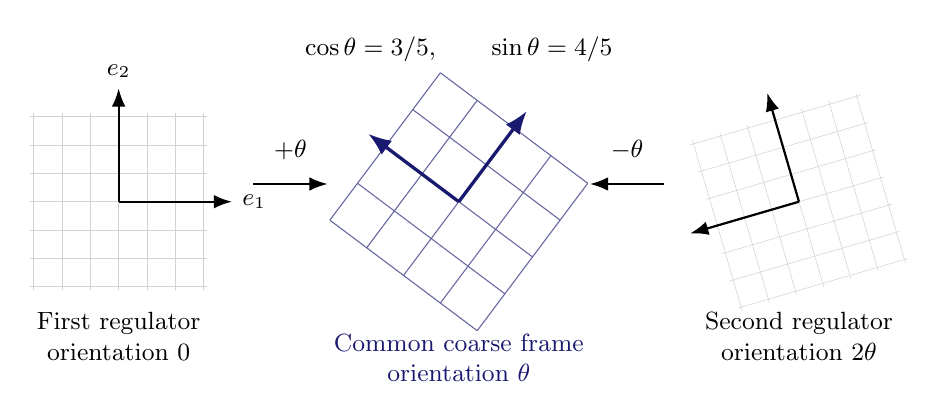
\begin{tikzpicture}[scale=0.9,>=Latex,every node/.style={font=\small}]
\begin{scope}[shift={(-4.8,0)}]
  \draw[step=.4,gray!35,very thin] (-1.25,-1.25) grid (1.25,1.25);
  \draw[->,thick] (0,0)--(1.6,0) node[right] {$e_1$};
  \draw[->,thick] (0,0)--(0,1.6) node[above] {$e_2$};
  \node[align=center] at (0,-1.9) {First regulator\\orientation $0$};
\end{scope}
\begin{scope}[rotate=53.130102]
  \draw[step=.65,MidnightBlue!65,thin] (-1.3,-1.3) grid (1.3,1.3);
  \draw[->,MidnightBlue,very thick] (0,0)--(1.6,0);
  \draw[->,MidnightBlue,very thick] (0,0)--(0,1.6);
\end{scope}
\node[align=center,text=MidnightBlue] at (0,-2.2)
  {Common coarse frame\\orientation $\theta$};
\begin{scope}[shift={(4.8,0)},rotate=106.260204]
  \draw[step=.4,gray!35,very thin] (-1.25,-1.25) grid (1.25,1.25);
  \draw[->,thick] (0,0)--(1.6,0);
  \draw[->,thick] (0,0)--(0,1.6);
\end{scope}
\node[align=center] at (4.8,-1.9) {Second regulator\\orientation $2\theta$};
\draw[->,thick] (-2.9,.25)--(-1.85,.25)
  node[midway,above=5pt,align=center] {$+\theta$};
\draw[->,thick] (2.9,.25)--(1.85,.25)
  node[midway,above=5pt,align=center] {$-\theta$};
\node at (0,2.15) {$\cos\theta=3/5,\qquad\sin\theta=4/5$};
\end{tikzpicture}
\caption{The two inclined first blockings produce the same physical
frame. Their relative inclinations are reflections of one another, so
their scalar field normalizations agree. After the first step, common
regular blockings erase the difference of their remaining data. The
drawing shows orientations only; the first coarse spacing is $5L$ times
the microscopic spacing.}
\label{fig:orientations}
\end{figure}


\emph{The two inclined blockings.}
Consider the fixed tilted square torus of side $5M$ and axes $O_+$
from Section~\ref{sec:trace}.  Put one microscopic regulator in the
standard axes and the other in axes $O_+^2$.  In their respective axes
use the inclined first steps $O_+$ and $O_-=O_+^{-1}$.  Their frames
then agree, because $O_+^2O_-=O_+$;
Figure~\ref{fig:orientations} shows these orientations.  Both regulators have the same
$\beta_N,a_N,B_N$ and compatible periods.

Stop at a fixed layer $j<N$.  If $B_N^*$ and $c_{i,N}^*$ denote the
inclined source normalizations, the exact source multiplier is now
\begin{equation}
       25L^{-2j}\frac{B_N}{B_N^*}
                    \prod_{i=1}^j(c_{i,N}^*)^{-1}.
 \label{eq:inclined-cell-source-multiplier}
\end{equation}
The factor $25$ comes from the area of the first block: the product of
the area factors through layer $j$ is $25L^{2(N-j)}$.  Reflection
covariance of the two inclined prescriptions makes the multipliers
in Equation~\eqref{eq:inclined-cell-source-multiplier} identical.
They are bounded at each fixed $j$ by
Proposition~\ref{prop:source-products} and the bounds on the individual
$c_{i,N}^*$.  Convergence of the ratio $B_N/B_N^*$ is not required.

Apply Equation~\eqref{eq:orig-14} and
Corollary~\ref{cor:source-endpoints} after the first step.  At the fixed
bottom layer, their generating functions differ by a quantity tending
to zero uniformly near the source origin, also when evaluated at the
common bounded multiplier
\eqref{eq:inclined-cell-source-multiplier}.  Explicitly, if $r_j>0$
is a common coarse-source comparison radius and $M_j$ bounds that
multiplier, restrict the physical cell sources to radius
$r_j/(2\max\{1,M_j\})$.  Their substituted arguments then lie in
radius $r_j/2$ for every $N$, so uniform convergence and Cauchy's
formula apply on one fixed polydisc without convergence of the
multiplier itself.  The common cell centers can
be chosen identical by translating the microscopic lattices.  Their
physical mesh can be fixed independently of $N$ at the chosen layer.
Every assigned microscopic point lies in its inclined first cell, so
the final descendants are within $C\,5L^{-j}$ of the common centers.
The same continuous-test approximation therefore proves equality of
the limiting moments, and hence of the finite-dimensional laws, on
this fixed tilted torus.  This step uses only the moment bounds for a
fixed tilted size.

\emph{Exchange of the cutoff and volume limits.}
For real $t_1,\ldots,t_r$ and compactly supported real tests
$f_1,\ldots,f_r$, set
\[
       F_N=\exp\!\left(i\sum_{\nu=1}^rt_\nu\phi_N(f_\nu)\right).
\]
It is a bounded local microscopic observable with $|F_N|=1$,
regardless of the size of $B_N$.  Once its support is contained in the
prescribed interior portion of an axis torus at doubling index $k$,
Section~\ref{sec:trace} gives
\begin{equation}
 \left|\E_{N,\mathrm{plane}}F_N
          -\E_{N,\mathrm{torus}(k)}F_N\right|
       \le C e^{-c2^k},
 \label{eq:characteristic-volume-comparison}
\end{equation}
uniformly in $N\ge K_0$.  The fixed-torus continuum limit has already
been proved.  The uniform moment bounds make the plane laws of this finite list tight.
For any subsequential plane limit, taking $N\to\infty$ in
Equation~\eqref{eq:characteristic-volume-comparison} bounds its
characteristic function within $Ce^{-c2^k}$ of the same fixed-torus
characteristic function.  Sending $k\to\infty$ identifies every
subsequential plane law.  This proves plane convergence and identifies
it with the successive torus and cutoff limit.  The same inequality
applied with $k=k(N)\to\infty$ gives every simultaneous axis exhaustion
claimed in the statement.  Uniform factorial moments give uniform
integrability, so moments converge along these limits as well.

For either regulator orientation, the trace-with-shift estimate of
Section~\ref{sec:trace} gives
Equation~\eqref{eq:characteristic-volume-comparison} also for the tilted
tori.  First take their fixed-size continuum limit, where the two
orientations have just been compared, and then send the doubling index
to infinity.  The resulting plane characteristic functions agree.
Because the comparison uses bounded characteristic functions, it
requires no moment bound uniform in the increasing tilted physical
size.
\end{proof}

\subsection{Euclidean symmetry and regularity}

Write $S_n^{\boldsymbol\alpha}$ for the plane moment measures just
constructed, and $S_n$ for the finite collection of their components.
There is no pointwise prescription for these correlation functions;
the following bounds specify their distributional meaning.

\begin{proposition}[Euclidean regularity]
\label{prop:euclidean-regularity}
The plane correlation functions are nonnegative Radon measures
componentwise, and for every scalar Schwartz test
$F\in\mathcal S((\R^2)^n)$ they satisfy
\begin{equation}
 |S_n^{\boldsymbol\alpha}(F)|
   \le C^n n!\,
       \sup_{x\in(\R^2)^n}
         \bigl[(1+|x|^2)^{2n}|F(x)|\bigr].
 \label{eq:orig-35}
\end{equation}
The lattice moment measures converge on Schwartz tests, with the same
bound.  Finite component norms can be incorporated by changing $C$.
The limiting correlations have permutation symmetry, internal $O(3)$
covariance, and invariance under all Euclidean isometries of $\R^2$.
Bounds for products of separately translated tests are uniform in
their separate translation parameters when the decay weights are
centered at those parameters.
\end{proposition}

\begin{proof}
The compact-test convergence and positivity from
Proposition~\ref{prop:continuum-limit} give nonnegative locally finite
measures.  Partition $\R^2$ into unit boxes indexed by $u\in\Z^2$.
On each such box the weights $(1+|x|^2)^{-2}$ and
$(1+|u|^2)^{-2}$ are comparable by a fixed constant.  Therefore
Equation~\eqref{eq:unit-box-majorant}, followed by summation of these
weights, gives
\[
 |S_n^{\boldsymbol\alpha}(F)|
  \le C^n n!\,
       \sup_{x_1,\ldots,x_n}
          \left[\prod_{i=1}^n(1+|x_i|^2)^2
                          |F(x_1,\ldots,x_n)|\right].
\]
Here the sum over product boxes factors into $n$ convergent sums, so
its cost is exponential in $n$.  Since
$\prod_i(1+|x_i|^2)^2\le(1+\sum_i|x_i|^2)^{2n}$, this proves
Equation~\eqref{eq:orig-35}.  The proof applies uniformly to the lattice
measures.  Cutting off a Schwartz test outside a large compact set
then gives convergence on Schwartz space: the weighted supremum of
the discarded tail tends to zero.  Replacing each weight by
$(1+|x_i-y_i|^2)^{-2}$ proves the assertion concerning separate
translations, with constants independent of $y_1,\ldots,y_n$.

Permutation symmetry and internal $O(3)$ covariance pass directly
from the lattice.  For a fixed physical translation, approximate its
displacement by lattice displacements.  The error on a smooth test
tends to zero by the majorants and test-space continuity.  Thus
translation invariance also passes to the limit.  The microscopic
reflections and quarter turns similarly give reflection and square
symmetry.

Let $\theta$ be the angle of $O_+$, so
$\cos\theta=3/5$.  Rotating the entire regulator rotates the arguments
of its moment functions.  The last assertion of
Proposition~\ref{prop:continuum-limit} therefore gives invariance under
rotation by $2\theta$.  This angle generates a dense subgroup of the
circle.  Indeed, if $\theta/\pi$ were rational, then
$e^{i\theta}$ would be a root of unity and
$2\cos\theta=6/5$ would be a rational algebraic integer, hence an
integer, a contradiction.  The same irrationality holds for
$2\theta/(2\pi)$.  Rotations act continuously on Schwartz test space;
Equation~\eqref{eq:orig-35} consequently extends this dense-subgroup
invariance to all rotations.  Together with reflections and
translations this is Euclidean invariance.
\end{proof}

The fourth-cumulant test in Section~\ref{sec:os} uses cell indicators before
approximating them by smooth functions.  The next estimate justifies
that approximation and also allows the microscopic cell boundaries to
move slightly with $N$.

\begin{lemma}[Boundary strips]
\label{lem:boundary-strips}
Fix an order $n$, a bounded region $K\subset\R^2$, and a bounded axis
rectangle $A$.  Let
$E_\varepsilon=K\cap\{x:\operatorname{dist}(x,\partial A)<\varepsilon\}$.
In the plane, uniformly in $N\ge K_0$ and in the microscopic origin,
\begin{equation}
 S_{n,N}^{\boldsymbol\alpha}
       (E_\varepsilon\times K^{n-1})
       \le C_{n,K,A}(\varepsilon+a_N).
 \label{eq:boundary-strip-bound}
\end{equation}
The same estimate holds on the axis tori, with the sets interpreted in
fixed bounded periodic charts.  It also holds with any one insertion
in the strip.  Consequently continuum convergence extends to products
of bounded axis-box indicators, to smooth approximations of these
indicators, and to cell boxes whose boundaries converge to the given
box boundaries.  More generally the same conclusion holds for bounded
Jordan measurable sets.
\end{lemma}

\begin{proof}
Choose a fixed bounded relative-coordinate box $D$ containing $K-K$.
Use coordinates in the regulator axes, so the full displacement lattice
is $a_N\Z^2$, regardless of the microscopic origin.  On a torus evaluate
translated spins periodically.  For a lattice site $x$, define
\[
 A_N(x)=(B_Na_N^2)^n
     \sum_{y_2,\ldots,y_n\in a_N\Z^2\cap D}
       \E\!\left[q_x^{\alpha_1}
                    \prod_{i=2}^n q_{x+y_i}^{\alpha_i}\right].
\]
For $n=1$ the sum and product over the other insertions are empty.
Every term is nonnegative.  Microscopic translation invariance makes
$A_N(x)$ independent of $x$; denote its value by $A_N$.  Notice that
all $n$ field-normalization factors and all $n$ lattice area factors
are included in $A_N$.

Let $Q$ be a fixed unit box.  Summing the first insertion over its
lattice sites and using positivity gives
\[
  \#(Q\cap\Lambda_N) A_N
     \le S_{n,N}^{\boldsymbol\alpha}
                  (Q\times(Q+D)^{n-1})
     \le C_{n,K}.
\]
The last inequality follows by a fixed unit-box covering and
Equation~\eqref{eq:unit-box-majorant}.  Since
$\#(Q\cap\Lambda_N)\ge c a_N^{-2}$, with a constant uniform over the
lattice origin, we obtain $A_N\le C_{n,K}a_N^2$.  If the first insertion
is in $E\subset K$, every choice of the other insertions in $K$ is
included in this relative-coordinate sum.  Hence
\begin{equation}
 S_{n,N}^{\boldsymbol\alpha}(E\times K^{n-1})
       \le C_{n,K}a_N^2\#(E\cap\Lambda_N).
 \label{eq:first-insertion-count}
\end{equation}
For a fixed rectangle boundary, elementary lattice counting gives
$a_N^2\#(E_\varepsilon\cap\Lambda_N)
 \le C_{K,A}(\varepsilon+a_N)$, proving
Equation~\eqref{eq:boundary-strip-bound}.

On a torus use the same displacement box $D$, with periodic evaluation
of $x+y_i$.  A fixed bounded displacement box can represent a periodic
site more than once, but its multiplicity is bounded at the fixed
physical scale under consideration.  The unit-box argument and the
moment bound therefore give the same estimate, with this fixed
multiplicity included in the constant.  Permutation symmetry treats
any insertion coordinate.

For completeness, if $A$ is merely bounded and Jordan measurable,
the lattice squares centered at points of
$\{\operatorname{dist}(x,\partial A)<\varepsilon\}$ are contained in the
$(\varepsilon+Ca_N)$-neighborhood of $\partial A$.  Thus the counting
term in Equation~\eqref{eq:first-insertion-count} is bounded by a
constant times the area of that neighborhood, which tends to zero as
$\varepsilon\downarrow0$ and $N\to\infty$.  Continuous inner and outer
approximations to the indicator now have arbitrarily small error in
every fixed-order correlation.  The error for a product of indicators
is bounded by the sum of the errors with one argument in a boundary
neighborhood.  Compact-test convergence applies to the continuous
approximants, and then the neighborhood widths tend to zero.  The same
argument covers moving boxes, since their symmetric differences lie
in shrinking neighborhoods of the limiting boundaries.
\end{proof}

\section{Reconstruction, mass gap, and non-Gaussian correlations}
\label{sec:os}

Section~\ref{sec:continuum} constructed the plane Schwinger functions
$S_n$ and proved their Euclidean covariance and growth bounds.  We now
verify the remaining reconstruction hypotheses and transfer the uniform
lattice decay estimate to the entire reconstructed Hilbert space.  A
separated four-point test will then show that the limiting field does not
satisfy Wick's rule.

Write $x=(x^0,x^1)$, with $x^0$ the Euclidean time coordinate, and put
$\theta(x^0,x^1)=(-x^0,x^1)$.  We use $\phi^a(f)$, $a\in\{1,2,3\}$, for
the limiting smeared fields supplied by
Proposition~\ref{prop:continuum-limit}.  Expectations of polynomials in
these variables are the corresponding pairings with the $S_n$.
For $s\in\R$, set
\[
 (\tau_s f)(x^0,x^1)=f(x^0-s,x^1),
 \qquad (\theta f)(x)=f(\theta x).
\]
The same notation $\tau_s$ denotes the induced translation of a field
polynomial.  Define $\Theta\phi^a(f)=\phi^a(\overline{\theta f})$ and
extend $\Theta$ multiplicatively and antilinearly to field polynomials.

\subsection{Reflection positivity and exponential clustering}

\begin{lemma}[Reflection positivity]
\label{lem:reflection-positivity}
Let $F$ be a polynomial in finitely many component fields
$\phi^a(f)$, where the smooth compactly supported tests $f$ have support
in $\{x^0>0\}$.  Then
\begin{equation}
 \E\bigl[(\Theta F)F\bigr]\ge0.
 \label{eq:continuum-reflection-positivity}
\end{equation}
This holds jointly for all three components.  The Schwinger functions
also satisfy the reality relations for a Hermitian multiplet and
$S_0=1$.
\end{lemma}

\begin{proof}
At every cutoff the nearest-neighbour measure is reflection positive
across microscopic site and link seams.  Since the union of the supports
appearing in $F$ is a compact subset of the open positive half-plane, a
microscopic seam within $O(a_N)$ of $\{x^0=0\}$ separates these supports
from their reflections for all sufficiently large $N$.  Evaluate $F$ on
the renormalized lattice fields and reflect about this seam.  Its
reflection-positive quadratic form is nonnegative.  The moment
convergence of Proposition~\ref{prop:continuum-limit} applies to each of
the finitely many terms in that form.  Replacing the microscopic
reflection by $\theta$ changes the tests by a translation of size
$O(a_N)$; Proposition~\ref{prop:moment-majorants} bounds the resulting
moment errors, which tend to zero.  Taking the limit proves
\eqref{eq:continuum-reflection-positivity}.  This argument permits
arbitrary component indices and polynomial coefficients, so it proves
joint positivity rather than separate componentwise positivity.
Reality and normalization pass through the same moment limits.
\end{proof}

The next estimate retains an exponent independent of the polynomial.
That uniformity will exclude low-energy states throughout the Hilbert
space, even though the constants multiplying the exponential depend on
the observables.

\begin{proposition}[Polynomial slab clustering]
\label{prop:slab-clustering}
There is $m>0$ with the following property.  Let $F$ and $G$ be fixed
polynomials in finitely many smooth compactly supported smeared
component fields.  If time translation separates the slabs containing
their supports by a distance $R\ge0$, then
\begin{equation}
 \bigl|\Cov(F,\tau_sG)\bigr|
       \le C_{F,G}e^{-mR}.
 \label{eq:polynomial-slab-clustering}
\end{equation}
The exponent $m$ is common to all such polynomials.  The Schwinger
functions satisfy the Euclidean clustering axiom also for Schwartz
tests.
\end{proposition}

\begin{proof}
Let $X_{i,N}$ denote the real smeared lattice fields entering the two
polynomials, with the translations needed to place their slabs.  Complex
tests may first be split into real and imaginary parts.  The factorial
moment bounds of Proposition~\ref{prop:moment-majorants}, uniformly in
$N$ and in translations of each fixed test, imply that for some
$\varepsilon>0$
\begin{equation}
 \sup_N \E\exp\Bigl(\varepsilon\sum_i|X_{i,N}|\Bigr)<\infty.
 \label{eq:polynomial-exponential-tails}
\end{equation}
Indeed, the even moment bounds give factorial bounds on all absolute
moments by Cauchy--Schwarz.  Summing the exponential series at a
sufficiently small radius gives an exponential moment for each variable;
H\"older's inequality combines the finitely many variables.  Neither
radius depends on the translation of a test.

For $M\ge1$, let $T_M(u)=\max(-M,\min(u,M))$ and form $F_{N,M}$ and
$G_{N,M}$ by replacing every real smeared field by its truncation
$T_M(X_{i,N})$.  If the polynomial degrees are $d_F,d_G$, then
\[
 \norm{F_{N,M}}_\infty\le C_F(1+M)^{d_F},
 \qquad
 \norm{G_{N,M}}_\infty\le C_G(1+M)^{d_G}.
\]
Equation~\eqref{eq:polynomial-exponential-tails} also gives
\begin{equation}
 \norm{F_N-F_{N,M}}_{L^2}
 +\norm{G_N-G_{N,M}}_{L^2}
 \le C_{F,G}e^{-c_{F,G}M},
 \label{eq:polynomial-truncation}
\end{equation}
with uniformly bounded $L^2$ norms for $F_N,G_N$.  To obtain this bound,
expand the polynomial difference into terms supported on
$\{\max_i|X_{i,N}|>M\}$.  Each term is bounded by a fixed polynomial in
$\sum_i|X_{i,N}|$; the exponential moment absorbs its square and the tail
indicator.  Cauchy--Schwarz then shows that replacing the covariance by
that of the truncated variables costs at most
$C_{F,G}e^{-c_{F,G}M}$.

The truncated variables remain bounded local lattice observables in the
same slabs.  Equation~\eqref{eq:orig-26} supplies a fixed physical decay
rate $\mu>0$.  The number of microscopic edges between the slabs,
multiplied by $a_N$, differs from $R$ by at most $O(a_N)$; this rounding
cost is bounded uniformly.  Consequently
\[
 |\Cov(F_N,\tau_sG_N)|
 \le C_{F,G}(1+M)^{d_F+d_G}e^{-\mu R}
       +C_{F,G}e^{-c_{F,G}M}.
\]
Set $M=1+R^2$.  The polynomial prefactor in the first term is absorbed
by $e^{\mu R/2}$, with a constant depending on the degrees.  The second
term is also at most a test-dependent constant times $e^{-\mu R/2}$.
Thus the estimate holds with the common choice $m=\mu/2$.  Moment
convergence passes it to the limiting fields.

Euclidean rotation invariance, proved in
Proposition~\ref{prop:euclidean-regularity}, gives clustering when one
compact collection of insertions is translated to infinity in any
direction.  The constants can be kept uniform as that direction varies:
the rotated tests have uniformly bounded suprema and supports in a
common bounded set, so the unit-box moment bounds give a common radius
in \eqref{eq:polynomial-exponential-tails}.  Their polynomial degrees
and coefficients are unchanged.  To extend this assertion to Schwartz tests, first approximate
them by compactly supported product tests.  At every fixed order, the
product-of-unit-box majorants used to prove
Equation~\eqref{eq:orig-35} bound the approximation errors uniformly in
the translation: place the polynomial weights separately around the
origins of the two translated collections.  Finite sums of product
tests are dense in the corresponding Schwartz test spaces.  The same
uniform bounds therefore allow approximation first and translation to
infinity second, proving the full clustering axiom.
\end{proof}

\subsection{Osterwalder--Schrader reconstruction and the full gap}

\begin{proposition}[Relativistic reconstruction]
\label{prop:os-reconstruction}
The Schwinger functions $S_n$ reconstruct a tempered Wightman theory in
$1+1$ dimensions with a three-component Hermitian scalar field.  Its
Hilbert space $\mathcal H$ is positive, its fields are local, and its
unitary representation of the Poincar\'e group satisfies the spectrum
condition.  The vacuum $\Omega$ is unique and normalized.  In the
positive-time reflection realization of $\mathcal H$, Euclidean time
translations induce a strongly continuous semigroup
$e^{-sH_{\rm phys}}$, $s\ge0$, with $H_{\rm phys}\ge0$ and
$H_{\rm phys}\Omega=0$.
\end{proposition}

\begin{proof}
We apply the Osterwalder--Schrader reconstruction theorem under the
linear growth condition~\cite[Section~IV.1]{OS75}.  We specify its regularity
hypothesis to make clear that the distributional construction in
Section~\ref{sec:continuum} suffices.  For $F$ on $(\R^2)^n$, use the
Schwartz seminorm
\[
 |F|_p=\max_{|\alpha|\le p}\sup_x
       (1+|x|^2)^{p/2}|\partial^\alpha F(x)|.
\]
The linear growth condition requires a bound
$|S_n(F)|\le \sigma_n|F|_{sn}$ with fixed $s$ and
$\sigma_n\le A(n!)^D$ for fixed $A,D$.  Equation~\eqref{eq:orig-35}
gives this with $s=4$: its weighted supremum is the zero-derivative part
of $|F|_{4n}$, and $C^n n!\le A(n!)^D$ after increasing $A,D$.

Restricting to Schwartz tests flat on the coincidence diagonals
(all derivatives vanish whenever $x_i=x_j$) gives precisely the test
class defined in \cite[Section~II, following Equation~(2.1), p.~284]{OS75}.
Normalization and reality follow
from Lemma~\ref{lem:reflection-positivity}; permutation symmetry and
Euclidean invariance follow from
Proposition~\ref{prop:euclidean-regularity}; joint positive-time
reflection positivity follows from the same lemma, extended by
test-space continuity; and clustering is
Proposition~\ref{prop:slab-clustering}.  These are the normalized
Euclidean axioms with the required linear growth bound.

The theorem applies to a finite Hermitian multiplet with
scalar spacetime transformation law; see \cite[Section~I, Remark~5]{OS75}.
More explicitly, the test
functions carry indices $a_1,\ldots,a_n\in\{1,2,3\}$; reflection
positivity holds for arbitrary combinations of these indices, while
summing the component bounds costs at most an exponential factor in
$n$, already allowed by the preceding factorial estimate.  Thus the
multilinear reconstruction has a single positive Hilbert space and the
asserted three-component field.  Clustering gives uniqueness of the
vacuum.  The positive-time reflection realization and its translation
semigroup are part of this reconstruction.  This application uses
smeared distributions throughout and requires neither Euclidean point
fields nor a prescription for equal-time products.
\end{proof}

The uniform exponent in Proposition~\ref{prop:slab-clustering} now
controls every state generated by time-ordered fields.  Positivity of
spectral measures extends the resulting exclusion of low energies to
the Hilbert-space closure.  This is the same spectral implication as
in \Rref{prop:continuum}; we give the argument for the present
reconstructed states.

\begin{proposition}[Gap above the vacuum]
\label{prop:continuum-gap}
For the Hamiltonian in Proposition~\ref{prop:os-reconstruction}, the
vacuum complement obeys
\begin{equation}
 H_{\rm phys}\big|_{\Omega^\perp}\ge m>0,
 \label{eq:orig-36}
\end{equation}
where $m$ is the common exponent of
Proposition~\ref{prop:slab-clustering}.
\end{proposition}

\begin{proof}
We first justify the density of states to which the slab estimate
applies.  Coincidence-flatness does not imply flatness on a surface
where two times agree but the spatial coordinates differ.  The positive
position measures and Euclidean rotations nevertheless allow us to
remove these surfaces in the reflection norm.

Spacetime rotations act only on the insertion coordinates, since
the three internal components are spacetime scalars.  Thus each
fixed-index component measure of $S_k$ is separately rotation
invariant.  For any such measure $\mu_k$ and $i\ne j$, set
\[
 A_{ij}=\{x:x_i^0=x_j^0,\ x_i\ne x_j\}.
\]
Let $B$ be a ball centred at the origin in $(\R^2)^k$.  It has finite
$\mu_k$-mass by Proposition~\ref{prop:moment-majorants} and is
invariant under simultaneous spacetime rotations.  For each
configuration with $x_i\ne x_j$, only finitely many rotation angles
make the time component of $x_i-x_j$ vanish.  Rotation invariance and
Tonelli's theorem therefore give
\[
 \mu_k(A_{ij}\cap B)
  =\frac1{2\pi}\int_B\int_0^{2\pi}
       \mathbf 1_{A_{ij}}(O_\alpha x)\,\dd\alpha\,\dd\mu_k(x)=0.
\]
Here $O_\alpha$ acts on every insertion coordinate.  Increasing the
ball shows that each equal-time surface has measure only on its full
coincidence diagonal.

The OS construction uses ordered positive-time tests; see
\cite[Section~V, following Equation~(5.2)]{OS75}.  One may also begin
with all coincidence-flat tests supported in positive time.  We show
that their reflection completion is the same.  Truncation at infinity
and away from the time-zero boundary reduces this comparison to
compactly supported tests in the latter class;
the smooth positive-time support condition and rapid decrease justify
these cutoffs in Schwartz topology, and the growth bounds imply
continuity of the reflection form.  Let $f_n$ be one of these compact
tests, with the coincidence-flatness used in reconstruction, and write
$[f_n]$ for its class for the reflection form.  Choose
a smooth even function $\chi_\varepsilon$ that is zero on
$[-\varepsilon,\varepsilon]$ and one outside
$[-2\varepsilon,2\varepsilon]$, with values in $[0,1]$, and put
\[
 f_{n,\varepsilon}(x)
   =f_n(x)\prod_{i<j}\chi_\varepsilon(x_i^0-x_j^0).
\]
The difference $f_n-f_{n,\varepsilon}$ tends to zero off the internal
equal-time surfaces.  Those surfaces have zero componentwise
$S_{2n}$-mass away from full coincidences, as just proved, and $f_n$
vanishes on the latter.  In the reflection form the positive and
reflected negative time arguments are separated from one another.
The integrands defining the squared reflection norm of this difference
thus tend to zero almost everywhere for every component measure of
$S_{2n}$.  They are bounded by a fixed constant on a common compact
set.  Dominated convergence proves
\[
 \norm{[f_n]-[f_{n,\varepsilon}]}\longrightarrow0.
\]
This approximation is in the reflection norm; it does not assert
Schwartz density after cutting equal-time surfaces.

The support of $f_{n,\varepsilon}$ lies in finitely many strict time
chambers.  Split it according to the ordering and use permutation
symmetry, permuting component indices with insertion coordinates, to
put each term in $0<x_1^0<\cdots<x_n^0$.  A compact subset
of this chamber is covered by finitely many product boxes whose time
intervals are disjoint and ordered.  A partition of unity and
product-test approximation in these boxes give finite sums of products
of smooth compactly supported one-field tests, converging in Schwartz
topology and hence in reflection norm.  Finite component sums obey the
same argument.  These compact time-ordered product states are dense in
the OS space $\mathcal H$, and the approximation also identifies the
completion of the larger coincidence-flat positive-time test class isometrically with
$\mathcal H$.

Let $F$ be a finite sum of products of smeared fields, with each product
supported in strictly ordered, mutually disjoint positive-time
intervals, as constructed above.  Its test kernel is coincidence-flat.
Write $[F]$ for its reflection-space class in $\mathcal H$ and set
\[
 v=[F]-\E[F]\Omega.
\]
These centered vectors are dense in $\Omega^\perp$, and their semigroup
matrix elements are
\[
 \inner{v}{e^{-sH_{\rm phys}}v}
   =\E\bigl[(\Theta F)(\tau_sF)\bigr]
       -\overline{\E[F]}\E[F].
\]
For all sufficiently large $s$, the reflected and translated supports
lie in slabs separated by $s$ plus a fixed constant depending on $F$.
Apply Proposition~\ref{prop:slab-clustering} with first observable
$\overline{\Theta F}$ and second observable $F$, using the
sesquilinear covariance convention of Section~\ref{sec:trace}.  It implies
\begin{equation}
 0\le\inner{v}{e^{-sH_{\rm phys}}v}\le C_v e^{-ms}.
 \label{eq:os-vector-decay}
\end{equation}
For a finite sum of product states one applies the same estimate to
each of the finitely many cross terms; the exponent remains $m$.

Let $E_H$ be the spectral resolution of $H_{\rm phys}$ and
$\nu_v(B)=\inner{v}{E_H(B)v}$ its finite positive spectral measure.
For $0<m'<m$, positive measure in $[0,m')$ would give
\[
 \inner{v}{e^{-sH_{\rm phys}}v}
    =\int_{[0,\infty)}e^{-s\lambda}\,\dd\nu_v(\lambda)
    \ge e^{-sm'}\nu_v([0,m')),
\]
contradicting \eqref{eq:os-vector-decay} as $s\to\infty$.
Hence $E_H([0,m'))v=0$ for every centered vector in the dense set.
Since a spectral projection is bounded, it vanishes on all of
$\Omega^\perp$.  Taking $m'\uparrow m$ proves
\eqref{eq:orig-36}.
\end{proof}

\subsection{Surviving fields and a separated fourth cumulant}

It remains to verify that the vacuum complement is nonzero and that
the limiting field is non-Gaussian.  Both follow from observables at
the fixed terminal block scale.  This uses the same field
renormalization as the construction and the spectral estimate.

\begin{proposition}[Nontriviality and failure of Wick factorization]
\label{prop:non-gaussian}
For a sufficiently large fixed terminal coupling $H$, there exist four
smooth compactly supported real tests $f_1,\ldots,f_4$ with strictly
disjoint ordered time ranges for which
\begin{align}
 &\E\prod_{i=1}^4\phi^1(f_i)
 -\E[\phi^1(f_1)\phi^1(f_2)]\E[\phi^1(f_3)\phi^1(f_4)] \notag\\
 &\quad
 -\E[\phi^1(f_1)\phi^1(f_3)]\E[\phi^1(f_2)\phi^1(f_4)]
 -\E[\phi^1(f_1)\phi^1(f_4)]\E[\phi^1(f_2)\phi^1(f_3)]
 \ne0.
 \label{eq:nonzero-fourth-cumulant}
\end{align}
The reconstructed Hilbert space satisfies $\Omega^\perp\ne\{0\}$.
Consequently the spectral bottom on $\Omega^\perp$ is both positive
and finite.
\end{proposition}

\begin{proof}
Choose four distinct unit terminal cells at fixed bounded distances,
with gaps between their closed time intervals.  Their number,
placement, and separations are fixed independently of $H$ and of the
cutoff.  Translations of the block partitions, as allowed in
Section~\ref{sec:continuum}, realize this common physical placement.
Let $X_{i,N}$ be the first component of the renormalized field sum over
the descendants of cell $i$.

The local source estimate of Proposition~\ref{prop:source-step} and
the comparison in Equation~\eqref{eq:orig-34} give, on a fixed complex
neighbourhood of the origin,
\begin{equation}
 \E\exp\Bigl(\sum_{i=1}^4 z_iX_{i,N}\Bigr)
   =\E_\mu\exp\Bigl(\sum_{i=1}^4 z_iV_{Y_i}^1\Bigr)+o_H(1),
 \label{eq:cell-generating-comparison}
\end{equation}
uniformly in the cutoff and in the admitted axis tori.  Here $\mu$ is
the corresponding terminal spin law and $Y_i$ labels cell $i$.
Cauchy's formula transfers the uniform analytic error to each of the
fixed moments of order at most four.

For completeness, the alignment estimate
\eqref{eq:orig-23} controls the spins at these finitely many sites in
mean square.  If a nearest-neighbour path of length $\ell$ joins $Y_i$
to $Y_1$, then
\[
 \E_\mu|V_{Y_i}-V_{Y_1}|^2
 \le \ell\sum_{e\text{ on the path}}\E_\mu r_e^2
 \le \ell^2\bigl(Ct^2+4e^{-cHt^2}\bigr)=o_H(1).
\]
The path lengths are fixed; $t=t_0$ tends to zero and $Ht^2=p_0^2$
tends to infinity as $H\to\infty$.  Internal $O(3)$ invariance makes
each $V_Y$ uniformly distributed on $S^2$.  If $U$ has this law, then
\[
 \E U^1=0,\qquad \E(U^1)^2=\frac13,
 \qquad \E(U^1)^4=\frac15.
\]
The coordinates have absolute value at most one.  Telescoping a
product and using the preceding mean-square estimate therefore gives,
for every pair of distinct chosen cells and for the four-cell product,
\begin{equation}
 \E[X_{i,N}X_{j,N}]=\frac13+o_H(1),
 \qquad
 \E\prod_{i=1}^4X_{i,N}=\frac15+o_H(1).
 \label{eq:terminal-cell-moments}
\end{equation}
The first moments vanish exactly by internal symmetry.

The estimates are uniform on axis tori.  We may thus first take the
periodic infinite-plane limit at fixed cutoff and then the continuum
limit.  The descendants in a standard blocking are axis boxes;
Lemma~\ref{lem:boundary-strips} identifies their limits with the fixed
physical cells and justifies any converging displacement of their
boundaries.  Denote the resulting cell variables by $X_i$.  Their
fourth cumulant is
\begin{equation}
 \E\prod_{i=1}^4X_i
   -\sum_{\{\{i,j\},\{k,l\}\}}\E[X_iX_j]\E[X_kX_l]
   =\frac15-3\left(\frac13\right)^2+o_H(1)
   =-\frac{2}{15}+o_H(1),
 \label{eq:cell-fourth-cumulant}
\end{equation}
where the sum runs over the three pairings of $\{1,2,3,4\}$.
Choose $H$ sufficiently large that this quantity is nonzero.  This
choice depends only on the fixed cells and the earlier RG constants,
and can be made before the later choices of $M_0$ and $K_0$ in
Section~\ref{sec:trace}.

Approximate each cell indicator by bounded smooth tests whose
differences from the indicator are supported in shrinking boundary
strips.  The approximations can preserve the strict gaps between the
time ranges.  Lemma~\ref{lem:boundary-strips} makes every moment in
\eqref{eq:cell-fourth-cumulant} converge under this approximation.
Thus suitable smooth tests satisfy
\eqref{eq:nonzero-fourth-cumulant}.  Since they have separated ordered
times, these are Schwinger correlations in the domains used by
reconstruction.  Wick factorization of the reconstructed Wightman
functions would, by their Euclidean continuation, give Wick
factorization for these Schwinger correlations as well.  Equation
\eqref{eq:nonzero-fourth-cumulant} excludes it.

The same two-cell calculation can be made for unit cells reflected
across $x^0=0$, with both cells a positive distance from the seam.
Their first-component correlation is $1/3+o_H(1)>0$.  Apply reflected
smooth approximations to this pair.  For a suitable real test $f$
supported strictly in positive time,
\[
 \norm{[\phi^1(f)]}^2
   =\E\bigl[\phi^1(\theta f)\phi^1(f)\bigr]>0,
 \qquad
 \inner{\Omega}{[\phi^1(f)]}=\E\phi^1(f)=0.
\]
Hence $\Omega^\perp$ contains a nonzero vector $v$.  Its spectral
measure has total mass $\norm v^2>0$.  Since $[0,\infty)$ is the
increasing union of bounded intervals, some finite $E$ satisfies
$\nu_v([0,E])>0$.  The spectral bottom on $\Omega^\perp$ is therefore
finite, and Proposition~\ref{prop:continuum-gap} makes it positive.
\end{proof}

\begin{proof}[Completion of the proof of Theorem~\ref{thm:main}]
The shooting construction gives bare couplings $\beta_N\to\infty$.
The prescribed lattice spacings satisfy $a_N=L^{-N}\to0$, and the
source construction in Section~\ref{sec:sources} supplies the positive
field renormalizations $B_N$ for the standard nearest-neighbour $O(3)$
model.  The terminal kinetic coupling is the fixed number $H$ at unit
physical block length.
Proposition~\ref{prop:continuum-limit} establishes convergence of the
renormalized correlations and finite lists of smeared fields, with
infinite volume taken first or simultaneously along the specified torus
exhaustion.  Proposition~\ref{prop:euclidean-regularity} gives their
temperedness and Euclidean symmetries.

Proposition~\ref{prop:os-reconstruction} reconstructs the local,
unitary relativistic theory.  Its full Hamiltonian gap is
Proposition~\ref{prop:continuum-gap}, and
Proposition~\ref{prop:non-gaussian} proves that a nonzero vacuum
complement and a nonvanishing connected fourth correlation survive in
this same continuum limit.  In particular the physical gap is positive
and finite at the fixed scale of the construction.  Every limiting
observable uses the field renormalizations already prescribed from the
nearest-neighbour model; the blocking observations are integrated
exactly and introduce no additional microscopic physical fields.  The
construction adds no symmetry-breaking mass term.
\end{proof}

\part{Canonical scaling along all diverging couplings}
\section{Trajectories with a bounded bare offset}
\label{sec:trajectories}

The construction above chooses the microscopic coupling by prescribing
its value after the final blocking step.  To treat every sufficiently
large microscopic coupling, we instead allow a bounded displacement
from an explicit reference sequence.  We shall prove that all these
trajectories remain admitted.  We shall also identify which displacements
give the same effective density at every fixed layer as the microscopic
depth tends to infinity.  This second conclusion requires a summable
sensitivity estimate for the error in the kinetic increment.

\subsection{Common reference scales and canonical increments}

We keep the observations and representations of
Sections~\ref{sec:setup}--\ref{sec:rg}.  In particular, $L$ is a fixed
sufficiently large power of two, and
\[
 \gamma=\frac{\log L}{2\pi},\qquad
 H_j=H+\gamma j,\qquad
 \mathfrak m_j=\lceil(\log H_j)^2\rceil,\qquad
 p_j=(\log H_j)^{P_0},\qquad t_j=H_j^{-1/2}p_j.
\]
A depth-$N$ trajectory starts at $b_N=\beta$ and runs through layers
$N,N-1,\ldots,0$.  Its precise coupling is admitted at layer $j$ when
$b_j\in[H_j/2,2H_j]$, and strict admission means that both inequalities
are strict.  The reference scales, rather than $b_j$, determine the
geometric thresholds and masks throughout a comparison.

There are three trajectory types, denoted by $P\in\{r,+,-\}$.
Type $r$ uses only ordinary observations of side $L$.  Type $+$ or $-$
uses first the inclined observation of side $5L$ in
Section~\ref{sec:free}, with respective rotation
\[
 O_+=\frac15\begin{pmatrix}3&-4\\4&3\end{pmatrix},
 \qquad O_-=O_+^{-1},
\]
and then uses ordinary observations.  A history records the observations
already made, including their coordinate frames.  In a comparison we
identify the frames of the layer under consideration and use the same
ordinary observation in the remaining common steps.

We use the bulk formulas and their compatible finite-period
representations.  Compatibility means that every observation descends
to the corresponding quotient lattice, while admission of a period
requires its shortest nonzero translation to satisfy the lower bound
in Section~\ref{setup:scales}.  The comparisons below use common
reference scales and the common refinements and zero padding of
Section~\ref{sec:setup}.  They apply to bulk lists and simultaneously
to the finite-period lists whenever the periods being compared are
compatible.  In particular, one may fix a common terminal period and
compare the resulting common periods at all fixed bottom layers.

Recall briefly what the discrepancy measures.  A retained density has
the form \eqref{eq:setup-effective-density}: it contains the precise
kinetic coupling, a finite vector of canonical polynomial coefficient
lists, regular local errors, and a covering sum for configurations with
large bond differences.  The regular errors are bounded with eight
derivatives on their graph domains; the covering activities are bounded
by a sum over supports meeting a site.  Their caps are
\[
 \delta_j=H_j^{-2.05},\qquad w_j=\exp(-p_j^{1/4});
\]
the complete definitions are
\eqref{eq:setup-error-list-norm} and
\eqref{eq:setup-covering-norm}.  For two bulk representations, $u_j$ denotes
the positively weighted list discrepancy
\eqref{eq:setup-density-discrepancy}.  The regular-error difference
uses seven derivatives and is divided by $\delta_j$; the covering
difference is divided by $w_j$.  The canonical coefficients are
compared without their displayed powers of the precise coupling.
We put $\lambda_j=b_{2,j}-b_{1,j}$, where each precise coupling is
defined by its bulk extraction and is shared by the corresponding
compatible finite-period representations.

For a comparison that also involves finite periods, choose the common
terminal periods to be compared and follow each of them through the
layers.  Write $u_j^{\rm bulk}$ and $u_j^T$ for
\eqref{eq:setup-density-discrepancy} in the bulk and on the layer-$j$
period corresponding to terminal period $T$, respectively.  In this case we use
\begin{equation}
 u_j=\max\bigl\{u_j^{\rm bulk},\ \sup_Tu_j^T\bigr\}.
 \label{eq:offset-family-discrepancy}
\end{equation}
The supremum may be restricted to the finitely many periods in the
comparison, or taken over a compatible family obeying the common
admission bounds.  The estimates are uniform in periods, and
$\lambda_j$ and the history error are common to this whole family.
The cap bounds are preserved under this maximum; the step estimates
for this convention are justified below.  In particular a finite-period comparison always
retains control of the bulk data that determine the kinetic increment;
no norm on an isolated finite torus is used to bound a bulk extraction.
Fixed positive comparison weights give
\begin{equation}
 \|f_{2,j}-f_{1,j}\|_{7,j,A}\le C_L\delta_j u_j,
 \qquad u_j\le C_L
 \quad\hbox{for two representations obeying the common caps.}
 \label{eq:offset-discrepancy-caps}
\end{equation}
The volume scalar is omitted from $u_j$, as it cancels from normalized
expectations.

The order of parameters will matter.  Choose the contraction slack
$\upsilon>0$ small enough for Theorem~\ref{thm:rg-step} and so that
\begin{equation}
 \frac{\upsilon}{2}<\min\{1,\eta/(2\pi)\},
 \label{eq:offset-slack}
\end{equation}
where $\eta$ is the gain in Proposition~\ref{prop:preliminary}.
Choose the support and derivative requirements, $L$, the canonical
caps and comparison weights, and $P_0$ in the order specified in
Section~\ref{subsec:rg-closure}.  All logarithmic powers in the
estimates below are then fixed.  Two bounds on the bare displacement,
$R$ and $R'$, will be chosen below, before increasing $H$.
Constants denoted by $C_L$ may depend on these already fixed
representation parameters, but not on $H$, the depth, the layer,
the period, or the precise couplings in their bands.  Once $H$ has
been fixed, we allow constants denoted by $C_H$ to depend on it.

\begin{proposition}[Canonical increments and comparison estimates]
\label{prop:rg-input}
For every type $P\in\{r,+,-\}$, initialize the nearest-neighbor model
as in Section~\ref{sec:shooting}.  As long as the input couplings lie
in their admitted bands, the exact observations produce representations
with all renewed shape caps and the recursion
\begin{equation}
 b_{j-1}=b_j+\alpha^P_{N-j}
              +\frac{\kappa^P_{N-j}}{b_j}+\Delta_j,
 \qquad |\Delta_j|\le C_LH_j^{-1.05}.
 \label{eq:offset-flow}
\end{equation}
There are $C_L<\infty$, $0<\sigma_1<1$, and a number
$\kappa_\infty$ such that
\begin{equation}
 |\alpha_h^P+\gamma|+|\kappa_h^P-\kappa_\infty|
       \le C_L\sigma_1^h \qquad(h\ge0).
 \label{eq:offset-increment-convergence}
\end{equation}
These sequences are independent of the precise running couplings,
and remain fixed when $H$ is increased.  The two inclined types have
the same scalar sequences.

On common ordinary steps, with discrepancy variables defined above,
\begin{align}
 u_{j-1}&\le q u_j+C_L\operatorname{poly}(H_j)\epsilon_h
                        +e_j|\lambda_j|,\nonumber\\
 |\lambda_{j-1}-\lambda_j|
     &\le C_Lu_j+C_L\operatorname{poly}(H_j)\epsilon_h
                        +e_j|\lambda_j|,
 & e_j&=C_L(\log H_j)^C/H_j.
 \label{eq:offset-weak-comparison}
\end{align}
If the histories share their last $m$ ordinary observations,
$\epsilon_h$ may be taken to be $r_0^m$, where $r_0=A_0/L^2$.
The choices can be made with
\begin{equation}
 \max\{q,r_0\}<\rho<L^{-2+\upsilon}<1
 \label{eq:offset-contraction-width}
\end{equation}
and strict spare width.  Here $q$ and $\rho$ are fixed bounds valid
for every subsequent sufficiently large $H$.  The corresponding free kernels and their
lifts compare in the exponential kernel norms of
Proposition~\ref{prop:free-bounds} with the same history bound.
\end{proposition}

\begin{proof}
The initialization in Section~\ref{sec:shooting} has zero canonical
coefficients and zero regular errors; its covering construction obeys
the covering cap.  Theorem~\ref{thm:rg-step} renews these caps and
gives the coupling recursion whenever its input is admitted.  It
produces the output representation before the next coupling-band
condition is imposed, a fact that will permit a first-exit argument.

The prescription in Section~\ref{subsec:rg-canonical} assigns the
canonical coefficients to the finite triangular operation
$\mathbf P\mapsto\mathcal C_h(\mathbf P)$.  After the powers of
$b^{-1/2}$ have been sorted, that operation depends only on the
incoming canonical coefficients and the free history.  The remaining
difference from the exact integral is retained in the regular errors
and covering activities, with its affine correction in $\Delta$.
The orbit starting from zero therefore fixes the sequences
$\alpha_h^P,\kappa_h^P$ independently of the precise coupling and
of $H$.  Lemma~\ref{lem:rg-canonical-contraction} and the history
contraction in Proposition~\ref{prop:free-bounds} give their
exponential convergence, as in Section~\ref{sec:shooting};
Lemma~\ref{lem:kinetic-increment} identifies their common first
limit as $-\gamma$.  Reflection interchanges the two inclined
prescriptions and preserves these scalar extractions, so their
scalar sequences agree.  This does not identify their coefficient
tensors in a fixed coordinate frame.

Equation~\eqref{eq:offset-weak-comparison} follows from
\eqref{eq:orig-5} with the simultaneous bulk and period convention.
To verify this convention through the normalization, first compare
the raw lists in the bulk and on each selected period using the
dominating discrepancy \eqref{eq:offset-family-discrepancy}.
Extract the difference of the kinetic corrections from the bulk raw
lists, with the factor $Ct_{j-1}^{-2}$ in
Section~\ref{subsec:rg-closure}.  The same bulk corrections are then
used to normalize every finite-period output.  Their regular reset
costs $Ct_{j-1}^{2}$ times this difference, cancelling the extraction
factor; the other reset discrepancies are the history and coupling
terms already present in \eqref{eq:orig-5}.  Missing bulk corrections
on a given period keep their complete winding records and the spare
support exponent, as in the period argument of
Section~\ref{subsec:rg-closure}; their off-mask parts retain the
covering estimates.  These operations introduce only the fixed
normalization multipliers already allowed before choosing $L$.
Thus each output discrepancy is bounded by
$qu_j+C_L\operatorname{poly}(H_j)\epsilon_h+e_j|\lambda_j|$,
with a common contraction coefficient $q$ below $\rho$ after the
triangular weights and large parameters are chosen with spare width.
Taking their maximum proves the first family inequality;
the coupling inequality uses the bulk term directly.
The history and kernel conclusions are
Proposition~\ref{prop:free-bounds}.  The spare width in
\eqref{eq:offset-contraction-width} is the choice made in
Proposition~\ref{prop:endpoint-matching}.  The uniform $o_H(1)$
terms in the step estimates can be absorbed into a fixed upper
contraction bound $q$ strictly below $\rho$; increasing $H$ later
does not change either chosen rate.
\end{proof}

\subsection{Summable sensitivity of the kinetic error}

The coefficient $e_j$ in
\eqref{eq:offset-weak-comparison} tends to zero but is not summable
over layers.  For matching trajectories from their behavior at large
$j$, we need finer information about the noncanonical increment
$\Delta_j$.  The raw-error estimate used in the proof of the exact
step supplies it.

\begin{lemma}[Sensitivity of the extracted kinetic error]
\label{lem:sensitivity}
For two admitted compatible representation families, including their
prescribed bulk lists, on a common ordinary step with common reference
scales, the discrepancies in
Proposition~\ref{prop:rg-input} satisfy
\begin{equation}
 |\Delta_{2,j}-\Delta_{1,j}|
 \le C_L H_j^{-1.01}(u_j+|\lambda_j|)
             +C_L\operatorname{poly}(H_j)\epsilon_h.
 \label{eq:offset-sensitivity}
\end{equation}
The constant is uniform over the bulk prescriptions and their
compatible admitted finite-period representations, once $H$ is
sufficiently large.
\end{lemma}

\begin{proof}
Before the constant and affine terms of the regular remainder are
extracted, let $R_j^\Delta$ denote the layer-$(j-1)$, seven-derivative
norm of the difference of its two bulk raw lists.  The Taylor comparison proved in
Section~\ref{subsec:rg-closure} gives the estimate
\cite[Equation~(5.39)]{OpenAI-O4}, with the improved coefficient
$q_1=C/L^2+o_H(1)$ established there for $S^2$:
\begin{equation}
 R_j^\Delta\le q_1\delta_j^\Delta
   +C_L\operatorname{poly}(\mathfrak m_j,p_j)\delta_j
                      (\epsilon_h+\lambda_g)
   +C_Lg^{4.5}(u_j+\epsilon_h+\lambda_g).
 \label{eq:offset-raw-discrepancy}
\end{equation}
Here $\delta_j^\Delta$ is the unnormalized bulk input regular-error
discrepancy; $g$ may be taken comparable to either $b_{i,j}^{-1/2}$;
and $\lambda_g\le C_L|\lambda_j|/H_j$.  By
\eqref{eq:offset-discrepancy-caps},
$\delta_j^\Delta\le C_LH_j^{-2.05}u_j$, while
$g\le C_LH_j^{-1/2}$ in the common bands.

The affine coefficient is the linear second-derivative functional
\eqref{eq:setup-affine-coefficient}, evaluated in the bulk.  Once
the coordinate frames and reference domains have been identified,
this is the same functional on both raw lists; it does not change
with the free kinetic kernel.  The extraction estimate in
Section~\ref{subsec:rg-closure} therefore gives
\begin{equation}
 |\Delta_{2,j}-\Delta_{1,j}|
       \le C t_{j-1}^{-2}R_j^\Delta
       \le C_L H_j R_j^\Delta.
 \label{eq:offset-affine-extraction}
\end{equation}
There is no support-cardinality loss in this estimate: a unit affine
direction is bounded by the polynomially weighted directions in
\eqref{eq:setup-error-directions}, so its two derivative slots cost
only $t_{j-1}^{-2}$.  The seven derivatives in the discrepancy norm
are more than sufficient.  The final reset of the canonical
prefactors has zero affine Hessian, as verified in
Section~\ref{subsec:rg-closure}, and hence contributes no additional
kinetic extraction.  Bulk extraction also explains the uniformity
in the period: missing or folded corrections remain in the winding
lists instead of changing $\Delta_j$.  Equation~\eqref{eq:offset-affine-extraction}
uses the bulk raw-list discrepancy, which is bounded using
$u_j^{\rm bulk}\le u_j$ from
\eqref{eq:offset-family-discrepancy}.  The inclusion of this bulk
term is essential when some labels wind or disappear on a finite period.

Multiplying \eqref{eq:offset-raw-discrepancy} by $C_LH_j$ bounds its
nonhistory terms by
\[
 C_L(H_j^{-1.05}+H_j^{-1.25})u_j
 +C_L\bigl((\log H_j)^C H_j^{-2.05}
                         +H_j^{-2.25}\bigr)|\lambda_j|.
\]
Any remaining fixed logarithmic powers are absorbed by the strict
power margins when $H$ is increased.  In particular this is bounded
by $C_LH_j^{-1.01}(u_j+|\lambda_j|)$.  The history terms can be
bounded by $C_L\operatorname{poly}(H_j)\epsilon_h$, proving
\eqref{eq:offset-sensitivity}.  The argument uses the raw-error
comparison for $S^2$ from Section~\ref{subsec:rg-closure}, rather
than an application of an $O(4)$ step theorem to the present model.
\end{proof}

\subsection{Admission and retuning}

The exponentially decaying canonical transients define the finite
constants
\begin{equation}
 A_P=\sum_{h=0}^{\infty}(\alpha_h^P+\gamma),\qquad
 A_{\rm abs}=\max_{P\in\{r,+,-\}}
                  \sum_{h=0}^{\infty}|\alpha_h^P+\gamma|,
 \qquad d=A_+-A_r=A_--A_r.
 \label{eq:offset-transients}
\end{equation}
These constants are fixed before $H$ is increased.  Recall the
reference sequence from Section~\ref{sec:shooting}:
\begin{equation}
 \vartheta_j=H_j-\frac{\kappa_\infty}{\gamma}\log(H_j/H),
 \qquad
 \vartheta_j-\vartheta_{j-1}
       =\gamma-\frac{\kappa_\infty}{H_j}+O_L(H_j^{-2}).
 \label{eq:offset-profile}
\end{equation}
The bare offset of a depth-$N$ trajectory is
$s=\beta-\vartheta_N$.  Choose once and for all
\begin{equation}
 R>4(|d|+\gamma+1),\qquad
 R'>R+2A_{\rm abs}+2,\qquad I=(-R,R).
 \label{eq:offset-range}
\end{equation}
We shall use $|s|\le R$ for the limiting comparisons and the larger
range $|s|\le R'$ for retuning.  Both bounds have now been chosen
independently of $H$.

\begin{proposition}[Uniform admission for bounded offsets]
\label{prop:admission}
For $H$ sufficiently large, every depth $N\ge1$, every type
$P\in\{r,+,-\}$, and every bare coupling
$\beta=\vartheta_N+s$ with $|s|\le R'$ give a strictly admitted
trajectory.  Uniformly over these choices,
\begin{equation}
 b_j=\vartheta_j+D_j,\qquad
 \max_{0\le j\le N}|D_j|\le C_{L,R'}.
 \label{eq:offset-admission}
\end{equation}
Moreover,
\begin{align}
 D_{j-1}-D_j&=\alpha^P_{N-j}+\gamma+E_{j,N},\nonumber\\
 |E_{j,N}|&\le C_L\left[
 H_j^{-1.05}
 +H_j^{-2}\bigl(\log(2+H_j/H)+|D_j|\bigr)
 +H_j^{-1}\sigma_1^{N-j}\right],
 \label{eq:offset-error-recursion}
\end{align}
and
\begin{equation}
 \sup_{N,P,\,|s|\le R'}\sum_{j=1}^{N}|E_{j,N}|
       =o_H(1).
 \label{eq:offset-error-sum}
\end{equation}
The constants in \eqref{eq:offset-admission} stay bounded as $H$
is increased, with all earlier parameters fixed.
\end{proposition}

\begin{proof}
The starting coupling is strictly in band for $H$ large, uniformly
in $N$ and $|s|\le R'$.  Indeed, for $x\ge1$ the ratio
$\log x/x$ is bounded, and hence
$|\vartheta_N-H_N|/H_N\le C_L/H$.
Consider a trajectory down to a possible first output outside its
band.  Every step forming that output has an admitted input, so
\eqref{eq:offset-flow} applies.  On such an input,
\[
 \left|\frac1{b_j}-\frac1{H_j}\right|
 \le C_LH_j^{-2}
          \bigl(\log(2+H_j/H)+|D_j|\bigr).
\]
Subtract \eqref{eq:offset-profile} from the coupling recursion and
use \eqref{eq:offset-increment-convergence}.  This gives
\eqref{eq:offset-error-recursion}, including the step forming a
possible first exit.

The sums required for this estimate are uniform in depth:
\begin{align*}
 \sum_{j\ge1}H_j^{-1.05}&\le C_LH^{-0.05},&
 \sum_{j\ge1}H_j^{-2}&\le C_LH^{-1},\\
 \sum_{j\ge1}H_j^{-2}\log(2+H_j/H)&\le C_LH^{-1},&
 \sum_{j=1}^{N}H_j^{-1}\sigma_1^{N-j}&\le C_LH^{-1}.
\end{align*}
The first three follow by integral comparison for
$H_j=H+\gamma j$; the last follows from the geometric series and
$H_j\ge H$.  Let $M_D$ be the maximum of $|D_j|$ on the segment,
including its last output.  Summing from $D_N=s$ and using
\eqref{eq:offset-transients} gives
\[
 M_D\le R'+A_{\rm abs}+o_H(1)+C_LH^{-1}M_D.
\]
Take $H$ large enough to absorb the final term.  This bounds $M_D$
by a constant depending only on $L,R'$ and the previously fixed
parameters.  Since also
\[
 \sup_{j\ge0}\frac{|\vartheta_j-H_j|+C_{L,R'}}{H_j}
       \longrightarrow0\qquad(H\longrightarrow\infty),
\]
every output covered by this bound lies strictly in its band.
There can be no first exit, which proves admission and
\eqref{eq:offset-admission}.  Substitution of this uniform bound
for $|D_j|$ in \eqref{eq:offset-error-recursion}, followed by the
same four summations, proves \eqref{eq:offset-error-sum}.
\end{proof}

\begin{lemma}[Retuning at an arbitrary depth]
\label{lem:retuning}
After increasing $H$ once more, let an ordinary trajectory have any
depth $N\ge1$ and bare offset $|s|\le R$.  For every integer $K\ge1$
there is $s_K\in[-R',R']$ such that the ordinary trajectory of
depth $K$ with bare coupling $\vartheta_K+s_K$ has exactly the
same terminal coupling $b_0$.
\end{lemma}

\begin{proof}
For every trajectory in Proposition~\ref{prop:admission}, summing
\eqref{eq:offset-error-recursion} to zero gives
\begin{equation}
 \left|b_0-H-s\right|\le A_{\rm abs}+o_H(1).
 \label{eq:offset-terminal-range}
\end{equation}
Let $T_K(t)$ be the terminal coupling of the ordinary depth-$K$
trajectory started at $\vartheta_K+t$.  Proposition~\ref{prop:admission}
gives strict admission for the whole interval $[-R',R']$.
The continuity argument in the proof of Proposition~\ref{prop:shooting}
therefore makes $T_K$ continuous on this interval: the reference
thresholds are fixed, and the exact integrations and representation
maps are continuous in the precise coupling on each finite admitted
run.  Take $H$ so that the uniform $o_H(1)$ in
\eqref{eq:offset-terminal-range} has absolute value less than one.
By \eqref{eq:offset-range},
\begin{align*}
 T_K(-R')&\le H-R'+A_{\rm abs}+1
                  <H-R-A_{\rm abs}-1\le b_0,\\
 T_K(R')&\ge H+R'-A_{\rm abs}-1
                  >H+R+A_{\rm abs}+1\ge b_0.
\end{align*}
The intermediate value theorem supplies $s_K$.  No monotonicity or
uniqueness of the shooting map is needed.
\end{proof}

\subsection{Matching at each fixed layer}

Retuning gives an exact equality of terminal couplings at finite
depths.  A different comparison identifies limits without such a
retuning.  Its hypothesis compensates the transient displacement
$A_P$ associated with the choice of initial observation.

\begin{proposition}[Fixed-layer matching]
\label{prop:matching}
Fix $H$ sufficiently large as above.  For $i\in\{1,2\}$, let
$P_i\in\{r,+,-\}$ be fixed and let a sequence of depth-$N_{i,n}$
trajectories have bare couplings
$\vartheta_{N_{i,n}}+s_{i,n}$, where
$N_{i,n}\longrightarrow\infty$ and $|s_{i,n}|\le R'$.
Suppose
\begin{equation}
 (s_{2,n}+A_{P_2})-(s_{1,n}+A_{P_1})\longrightarrow0.
 \label{eq:offset-matching-hypothesis}
\end{equation}
Compare their bulk representations in common layer coordinates,
using the same ordinary observations on their common bottom steps.
Then, for every fixed integer $j\ge0$,
\begin{equation}
 u_{j,n}\longrightarrow0,\qquad
 \lambda_{j,n}\longrightarrow0.
 \label{eq:offset-fixed-layer-matching}
\end{equation}
The same statement holds on each fixed common compatible terminal
period and its corresponding bottom-layer periods.
\end{proposition}

\begin{proof}
All the trajectories are admitted by Proposition~\ref{prop:admission}.
At layer $j$, the histories share at least
$\min(N_{1,n},N_{2,n})-1-j$ most recent ordinary observations,
once the depths are sufficiently large.  Thus their history error
tends to zero at each fixed layer.  The normalized caps and
\eqref{eq:offset-admission} also give constants, independent of
$j,n$, bounding $u_{j,n}$ and $|\lambda_{j,n}|$ whenever the layer
is present.  Define
\[
 U_j=\limsup_{n\to\infty}u_{j,n},\qquad
 W_j=\limsup_{n\to\infty}|\lambda_{j,n}|.
\]
Both sequences are uniformly bounded.

We first establish the boundary condition for $W_j$ at large
layers.  The recursion in Proposition~\ref{prop:admission} gives
\[
 D_{i,j}=s_{i,n}
       +\sum_{h=0}^{N_{i,n}-j-1}(\alpha_h^{P_i}+\gamma)
       +\sum_{m=j+1}^{N_{i,n}}E_{i,m,N_{i,n}}.
\]
For fixed $j$ the transient sum tends to $A_{P_i}$ as
$n\to\infty$.  The error bound, with
\eqref{eq:offset-admission} substituted, gives
\begin{equation}
 W_j\le C_{L,R'}\sum_{m>j}
       \left[H_m^{-1.05}
          +H_m^{-2}\bigl(\log(2+H_m/H)+1\bigr)\right]
       +\frac{C_L}{H_j}.
 \label{eq:offset-boundary-at-infinity}
\end{equation}
Here \eqref{eq:offset-matching-hypothesis} cancels the two limiting
offsets, and the final term bounds each transient sum by
\[
 \sum_{m=j+1}^{N}H_m^{-1}\sigma_1^{N-m}
                 \le \frac1{H_j(1-\sigma_1)}.
\]
The right side of \eqref{eq:offset-boundary-at-infinity} tends to
zero as $j\to\infty$, with $H$ fixed.  Consequently
\begin{equation}
 W_j\longrightarrow0\qquad(j\longrightarrow\infty).
 \label{eq:offset-W-boundary}
\end{equation}
This argument does not require the complete error sum at fixed $H$
to vanish as the depth increases.

At each fixed $j\ge1$, take upper limits in the first inequality of
\eqref{eq:offset-weak-comparison}.  The history forcing disappears.
For the coupling, subtract \eqref{eq:offset-flow} for the two
trajectories and use Lemma~\ref{lem:sensitivity}.  At this fixed
layer the two $\alpha$ values tend to $-\gamma$ and the two
$\kappa$ values to $\kappa_\infty$.  The remaining denominator
variation is bounded by $C_LH_j^{-2}|\lambda_{j,n}|$.
It follows that
\begin{equation}
 U_{j-1}\le qU_j+e_jW_j,\qquad
 W_{j-1}\le W_j+a_j(U_j+W_j),\qquad
 a_j=C_LH_j^{-1.01}.
 \label{eq:offset-limsup-recursions}
\end{equation}

Put $U=\sup_{j\ge0}U_j$, $W=\sup_{j\ge0}W_j$, and
$e_* =\sup_{j\ge1}e_j$.  Iterating the first inequality through
$m$ layers above $k$ yields
\[
 U_k\le q^m U_{k+m}
             +W\sum_{r=1}^{m}q^{r-1}e_{k+r}.
\]
Boundedness and $q<1$ allow $m\to\infty$, giving
$U\le e_*W/(1-q)$.  Next sum the second inequality of
\eqref{eq:offset-limsup-recursions} from $k+1$ to $k+m$.
Letting $m\to\infty$ and using \eqref{eq:offset-W-boundary}
gives
\[
 W_k\le\sum_{j>k}a_j(U_j+W_j),\qquad
 W\le\left(\sum_{j\ge1}a_j\right)(U+W).
\]
No limit has been interchanged with an infinite sum: the limiting
recurrences were first obtained at fixed layers and then iterated.
Finally,
\[
 e_*\longrightarrow0,\qquad
 \sum_{j\ge1}a_j\le C_LH^{-0.01}\longrightarrow0
                  \qquad(H\longrightarrow\infty).
\]
We choose $H$, once for all the trajectories, so that
\[
 \left(\sum_{j\ge1}a_j\right)
                  \left(1+\frac{e_*}{1-q}\right)<1.
\]
The two supremum inequalities force $W=0$ and then $U=0$,
which proves \eqref{eq:offset-fixed-layer-matching}.  The proof
uses the bulk norms and the simultaneous finite-period norms from
Proposition~\ref{prop:rg-input}; it therefore applies to each fixed
compatible terminal period as stated.
\end{proof}

For later use, all further requirements that $H$ be large, including
the local source and terminal-alignment estimates, are imposed before
any depth or volume thresholds are selected.  The bounds $R,R'$,
the transient constants, and the reference prescriptions remain fixed
throughout these choices.

\section{Volume estimates uniform in the bare offset}
\label{sec:volume}

The trajectories admitted in Proposition~\ref{prop:admission} have
terminal couplings in a fixed band, but generally do not end at $H$.
We now extend the finite-volume estimates of Section~\ref{sec:trace}
to this entire family.  The argument first matches two trajectories
at their common terminal coupling, then transfers a rectangular
partition-function test from a retuned reference depth to every finer
cutoff.  The resulting bounds will allow local field comparisons on
fixed tori to pass to the plane.

\subsection{Positivity at finite coupling}
\label{sec:finite-beta}

We first record the elementary positivity needed to use component
moments as measures.  All torus partition functions retain the
normalization in \eqref{eq:lattice-model}: normalized area measure at
each site, and each unoriented nearest-neighbor bond counted once.

\begin{lemma}[Finite-coupling moments and normalization]
\label{lem:finite-beta}
For every sufficiently large fixed $\beta$, the periodic plane law
$\mu_\beta$ exists and is translation and $O(3)$ invariant.  Every
component moment
\[
 \E_{\mu_\beta}\prod_{r=1}^n q_{x_r}^{i_r},
 \qquad x_r\in\Z^2,\quad i_r\in\{1,2,3\},
\]
is nonnegative.  If
\[
 C_\beta(x)=\E_{\mu_\beta}[q_0^1q_x^1],\qquad
 \chi_\beta=\sum_{x\in\Z^2}C_\beta(x),\qquad
 \xi_\beta^2=\frac{\sum_x|x|^2C_\beta(x)}{4\chi_\beta},
\]
then both sums converge absolutely and
$0<\chi_\beta,\xi_\beta<\infty$, where $\xi_\beta$ is the positive
square root.  More precisely, $C_\beta(0)=1/3$ and, for each
nearest-neighbor vector $e$,
\begin{equation}
 C_\beta(e)\ge\frac{\beta}{9}e^{-7\beta}>0.
 \label{eq:offset-edge-positive}
\end{equation}
\end{lemma}

\begin{proof}
Proposition~\ref{prop:preliminary} gives the periodic plane limit.
The symmetries of its torus approximants pass to that limit; in
particular each component has mean zero.  Apply
\eqref{eq:prelim-mixing} to $q_0^1,q_x^1$ on arbitrarily large tori
at this fixed $\beta$, and then pass to the plane.  It gives
\[
 |C_\beta(x)|\le
 C(1+\beta+|x|)^p\exp[-c|x|/X(\beta)].
\]
The two sums in the statement therefore converge absolutely.

For positivity, expand each factor
$\exp(\beta\sum_{i=1}^3q_x^iq_y^i)$ in its componentwise power series
on a finite torus.  The series of absolute values is integrable,
since the spins are bounded and the torus has finitely many edges.
Every integrated term, including any prescribed component insertion,
factors into one-site monomial integrals.  Such an integral vanishes
if one coordinate exponent is odd and is nonnegative if all are
even.  All expansion coefficients are nonnegative.  Division by the
positive partition function, followed by the periodic limit, proves
the asserted moment positivity.

Consider one edge $\{0,e\}$ on a torus with sides at least four.
Exactly seven distinct bonds meet its two endpoints.  Delete these
bonds and denote the resulting partition function by $Z^{\rm del}$.
In the expansion of the numerator for $q_0^1q_e^1$, retain the term
$\beta q_0^1q_e^1$ from the chosen edge and the constant terms from
the other six incident bonds, leaving all nonincident expansions
unrestricted.  The isolated endpoint integrals each equal $1/3$,
so this contribution is $\beta Z^{\rm del}/9$.  Termwise
nonnegativity bounds the full numerator from below by this value.
Since the deleted interaction is at most $7\beta$ pointwise,
$Z\le e^{7\beta}Z^{\rm del}$.  This proves
\eqref{eq:offset-edge-positive}, also after passing to the plane.
Internal symmetry gives $C_\beta(0)=1/3$.  Nonnegativity now gives
$\chi_\beta\ge1/3$ and a strictly positive second-moment numerator.
\end{proof}

\subsection{Endpoint comparisons with a varying terminal coupling}

The reference scale at the endpoint remains $H$ throughout.  Thus the
thresholds are always $t_0=H^{-1/2}p_0$, the regular-error cap is
$\delta_0=H^{-2.05}$, and the covering cap is
$w_0=\exp(-p_0^{1/4})$.  These quantities are not replaced by
functions of the precise terminal coupling.

\begin{lemma}[Ordinary endpoint laws throughout the terminal band]
\label{lem:band-endpoints}
Fix a finite covering-cap multiplier and $C_0>0$ before choosing $H$
sufficiently large.  Let a trajectory obtained from the microscopic
Gibbs law by the exact ordinary observations satisfy the admission and
cap conditions of Section~\ref{sec:setup}, with terminal coupling
$b_0\in[H/2,2H]$.  On a standard terminal axis torus of bounded
aspect, with the lower bounds and divisibilities of
Section~\ref{sec:comparison}, its scalar-stripped endpoint density
is an admissible base for Proposition~\ref{prop:integrated-comparison}
and Corollary~\ref{cor:terminal-alignment}, with constants uniform in
the trajectory, its depth, its period, and $b_0$ in this band.
In particular, every endpoint bond obeys
\begin{equation}
 \mu\{|q_x-q_y|>t_0/C_0\}\le e^{-cHt_0^2}
 \label{eq:offset-terminal-alignment}
\end{equation}
for a corresponding $c>0$.
The integrated comparison also permits complex comparison weights
whose support-hit envelope obeys the chosen multiplier of the covering
cap, as in its original statement.
\end{lemma}

\begin{proof}
The definition in Section~\ref{setup:endpoints}, specifically
\eqref{setup:endpoint-law}, already allows a precise coupling in
$[H/2,2H]$.  An actual observed law is positive because its density
is the integral of the positive microscopic density against positive
normalized observations.  The ordinary observations on the two
sides of a retained seam are independent and are exchanged by
reflection.  The verification at the end of
Section~\ref{sec:shooting} therefore supplies link reflection
positivity without any condition $b_0=H$.

The quantitative estimates used in the integrated comparison have
the same uniformity.  In Lemma~\ref{lem:comparison-remainder},
group the kinetic rows with their precise coupling $b_0$.  The omitted
tails cost at most $2H$ times the exponentially small kernel tail,
and the canonical contributions remain bounded by
$C_L(Ht_0^4+t_0^2)$ per anchor.  In
Lemma~\ref{lem:editable-regions}, the lower and upper energy bounds
use respectively $b_0\ge H/2$ and $b_0\le2H$; their energy scale is
still $Ht_0^2=p_0^2$.  The sampling, masks, complete supports, and
inventory constraints have the same reference thresholds and caps.
The chessboard argument uses only the seam reflection positivity and
the even tile counts, both just checked.  These are precisely the
hypotheses of Proposition~\ref{prop:integrated-comparison}.
The disseminated-event proof of
Corollary~\ref{cor:terminal-alignment} uses the same remainder and
partition-function bounds and the lower kinetic bound $b_0\ge H/2$.
It therefore gives \eqref{eq:offset-terminal-alignment} uniformly.
\end{proof}

\begin{proposition}[Endpoint comparison at a common terminal value]
\label{prop:endpoint-comparison}
Fix $L,R,R'$ and choose $H$ sufficiently large as in
Proposition~\ref{prop:admission}.  Consider two admitted ordinary
trajectories of depths $N\ge K\ge1$, with offsets bounded by $R'$,
common reference scales and caps, and the same precise terminal
coupling $b_0$.  Align their last $K$ layers on common compatible
periods.  Write their scalar-stripped endpoint densities as
$e^{X_i}\Xi_i$.  On each common admitted terminal torus of volume
$v$, their common refined activity lists satisfy
\begin{align}
 \|X_1-X_2\|_\infty
    &\le C_Hv\epsilon_K,\notag\\
 \sup_x\sum_{\lambda:x\in P_\lambda}
 e^{As_\lambda}\|k_{1,\lambda}-k_{2,\lambda}\|_\infty
    &\le C_H\epsilon_K,
 \qquad \epsilon_K=L^{-(2-\upsilon)K}.
 \label{eq:offset-endpoint-comparison}
\end{align}
Here $P_\lambda$ and $s_\lambda$ are the complete support and load
of a covering label, and $A$ is the support exponent of the endpoint
class.  If the common torus is an axis torus satisfying
Lemma~\ref{lem:band-endpoints} and $C_Hv\epsilon_K$ is sufficiently
small, its scalar-stripped partition functions satisfy
\begin{equation}
 |\log\widehat Z_1-\log\widehat Z_2|
       \le C_Hv\epsilon_K.
 \label{eq:offset-endpoint-logZ}
\end{equation}
The constants are independent of $N,K$, the periods, and the common
terminal value.
\end{proposition}

\begin{proof}
We verify the uniformity in the common terminal value in the
two-boundary proof of Proposition~\ref{prop:endpoint-matching}.
The normalized discrepancies $u_j$ and precise-coupling differences
$\lambda_j$ are those of \eqref{eq:setup-density-discrepancy}.
The equality of the terminal couplings is exactly $\lambda_0=0$.
The shared ordinary tail gives history error at most
$r_0^{K-j}$, by Proposition~\ref{prop:free-bounds}, with
$r_0=A_0/L^2$.  Thus Theorem~\ref{thm:rg-step} gives, for
$1\le j\le K$,
\[
 u_{j-1}\le q u_j+e_*|\lambda_j|+f_j,
 \qquad
 |\lambda_j|\le a_*|\lambda_{j-1}|+a_*C_Lu_j+a_*f_j,
\]
where
\[
 e_* = \sup_{j\ge1}C_L(\log H_j)^C/H_j=o_H(1),
 \quad a_*=(1-e_*)^{-1},\quad
 f_j\le C_L\operatorname{poly}(H_j)r_0^{K-j}.
\]
Choose $\max(q,r_0)<\rho<L^{-2+\upsilon}$ with strict spare width,
and put $F_K=C_H(1+K)^C$, large enough that
$f_j\le F_K\rho^{K-j}$.  For
\[
 U=\max_{0\le j\le K}\frac{u_j}{\rho^{K-j}},
 \qquad W=\max_{0\le j\le K}
                  \frac{|\lambda_j|}{\rho^{K-j}},
\]
downward iteration for $u$ and upward iteration from $\lambda_0=0$
give
\[
 U\le u_K+\frac{e_*W+F_K}{\rho-q},
 \qquad
 W\le\frac{a_*(C_LU+F_K)}{1-a_*\rho}.
\]
Choose $H$ so that $a_*\rho<1$ and the product of the two
coefficients coupling $U,W$ is less than $1/2$.
The common caps bound $u_K$, so
$u_j+|\lambda_j|\le C_H(1+K)^C\rho^{K-j}$.
This calculation uses no specified value of $b_0$ beyond its band.

At layer zero the conversion in the proof of
Proposition~\ref{prop:endpoint-matching} uses the coefficient norms,
masked regular norms, complete-support load bounds, and free-history
kernel bounds.  These are the common reference norms just used.
It gives \eqref{eq:offset-endpoint-comparison}, absorbing the factor
$(1+K)^C$ in the spare exponential width.  All regular supremum bounds
remain on their prescribed masks; common-list refinements keep their
exact covering corrections.

For the partition functions, set
$\varepsilon=C_Hv\epsilon_K$.  Summing the support-hit bound gives
\[
 \sum_\lambda e^{2s_\lambda}
       \|k_{2,\lambda}-k_{1,\lambda}\|_\infty\le\varepsilon.
\]
By Lemma~\ref{lem:band-endpoints} and
Proposition~\ref{prop:integrated-comparison},
\[
 \left|
 \frac{\int e^{X_1}\Xi_2\dd q}{\widehat Z_1}-1
 \right|\le e^{\varepsilon}-1.
\]
Both actual densities are positive, hence $\Xi_2>0$.
The exponent bound therefore compares $\widehat Z_2$ with
$\int e^{X_1}\Xi_2\dd q$ by factors between
$e^{-\varepsilon}$ and $e^{\varepsilon}$.  For small $\varepsilon$
taking logarithms proves \eqref{eq:offset-endpoint-logZ}.
Each extracted bulk scalar is exactly per volume and independent of
the period, by \eqref{eq:setup-effective-density}; winding
corrections remain in the density.  This fact will allow the scalars
to cancel in the doubling test.
\end{proof}

\subsection{One reference box for every offset}

Recall the rectangular test from \eqref{eq:trace-doubling-definition},
\[
 \Delta_\beta(n,w)=4\log Z_\beta(n,w)-\log Z_\beta(2n,2w).
\]
For later plane comparisons we use
\begin{equation}
 \begin{split}
 \mathcal A&=\{(1,1),(1,25)\},\\
 \mathcal U&=\mathcal A
 \cup\{(u_1/2,u_2):(u_1,u_2)\in\mathcal A\}
 \cup\{(2u_1,u_2/2):(u_1,u_2)\in\mathcal A\}.
 \end{split}
 \label{eq:offset-aspect-inventory}
\end{equation}
The auxiliary aspects are needed when one doubles the time period
and then the spatial period.  The aspect $(1,25)$ will also cover
the inclined microscopic tori.

\begin{lemma}[A reference-box test uniform in the offset]
\label{lem:offset-box-test}
The contraction slack $\upsilon>0$ and then the parameters may be
chosen so that there exist integers $K_0,M_0\ge1$ with
\begin{equation}
 0\le\Delta_\beta(u_1M_0L^N,u_2M_0L^N)\le2^{-10}
 \label{eq:offset-box-test}
\end{equation}
whenever $N\ge K_0$, $\beta=\vartheta_N+s$, $|s|\le R$, and
$(u_1,u_2)\in\mathcal U$.  The integer $M_0$ may be required to
exceed any fixed lower bound and to be divisible by any fixed
integer.  In particular all displayed half-periods and all tile
counts required in Section~\ref{sec:comparison} can be even.
\end{lemma}

\begin{proof}
Let $\eta>0$ be the gain in Proposition~\ref{prop:preliminary}.
Choose the slack small enough to admit a number $z$ with
\begin{equation}
 0<\upsilon/2<z<\min\{1,\eta/(2\pi)\}.
 \label{eq:offset-box-exponents}
\end{equation}
Fix all large-$H$ requirements, including
Lemma~\ref{lem:band-endpoints}, before choosing the box sizes.
Take $m_K$ to be a fixed common integer multiple of a rounded
dyadic integer with
\[
 \log_L m_K=(1-z)K+O(1).
\]
The fixed multiple clears the denominators of $\mathcal U$ and
imposes the divisibilities and lower bounds in the statement.

For each depth-$N$ ordinary run with $|s|\le R$, and each $K\le N$,
Lemma~\ref{lem:retuning} supplies a depth-$K$ ordinary run with
bare coupling $\widetilde\beta_K=\vartheta_K+\widetilde s_K$,
$|\widetilde s_K|\le R'$, and exactly the same terminal coupling.
Uniformly over these retunings,
\[
 \widetilde\beta_K=H+\gamma K+O_{H,L,R'}(\log(2+K)),\qquad
 X(\widetilde\beta_K)
 \le C_H(1+K)^C L^{(2-\eta/(2\pi))K}.
\]
The shorter side of $(u_1,u_2)m_KL^K$ is comparable to
$L^{(2-z)K}$.  Its ratio to this preliminary upper length grows
exponentially, by $z<\eta/(2\pi)$.  The even periods thus satisfy
all hypotheses of \eqref{eq:prelim-doubling}, whose exponentially
small factor dominates its polynomial prefactor.  Consequently
\[
 \sup_{\substack{N\ge K,\ |s|\le R\\(u_1,u_2)\in\mathcal U}}
 \Delta_{\widetilde\beta_K}(u_1m_KL^K,u_2m_KL^K)
       \longrightarrow0.
\]

Run both cutoffs to their common terminal rectangle
$(u_1,u_2)m_K$, of volume $v=u_1u_2m_K^2$, and do the same on
the doubled rectangle.  These periods are admitted: the imposed
terminal lower bound and the growth of the periods through earlier
layers give the conditions in Section~\ref{setup:scales}.
Proposition~\ref{prop:endpoint-comparison} applies, because the two
terminal couplings agree.  Since
\[
 m_K^2\epsilon_K
 =L^{(\upsilon-2z)K+O(1)}\longrightarrow0,
\]
its partition-function estimates are applicable for large $K$.
The per-volume scalars cancel separately in each rectangular test,
giving
\begin{align*}
 &\left|\Delta_{\beta}(u_1m_KL^N,u_2m_KL^N)
       -\Delta_{\widetilde\beta_K}(u_1m_KL^K,u_2m_KL^K)\right|\\
 &\hspace{35mm}\le C_Hm_K^2\epsilon_K\longrightarrow0
\end{align*}
uniformly over the displayed family.  Choose one sufficiently large
$K_0$ and set $M_0=m_{K_0}$.  Nonnegativity of the tests follows
from the two-direction transfer identities
\eqref{eq:trace-rectangle-identities}.  This proves
\eqref{eq:offset-box-test}.
\end{proof}

\subsection{Transfer bounds and the plane limit}

Only the finite list of tests in Lemma~\ref{lem:offset-box-test}
is needed from renormalization for the next result.  The rest is the
positive-transfer argument of Section~\ref{sec:trace}, now applied
uniformly to the offset family.

\begin{proposition}[Uniform volume comparison and slab decay]
\label{prop:uniform-volume}
Fix $K_0,M_0$ as in Lemma~\ref{lem:offset-box-test}.  There exist
$C,c>0$, independent of $N\ge K_0$, $|s|\le R$, and $k\ge0$,
such that the following hold for $\beta=\vartheta_N+s$.

Let $(u_1,u_2)\in\mathcal A$ and
$(n,w)=(u_1,u_2)2^kM_0L^N$.  If a bounded local observable $F$
has support contained in a rectangle of time extent at most $n/2$
and spatial extent at most $w/2$, then
\begin{equation}
 |\mu_{\beta;n,w}(F)-\mu_\beta(F)|
       \le C\|F\|_\infty e^{-c2^k}.
 \label{eq:offset-uniform-volume}
\end{equation}
The same bound holds when time is closed by any integer spatial
translation, provided the support has a lift satisfying these two
extent bounds.  The constant is uniform in the closing translation.

If two bounded local plane observables $F,G$ have supporting slabs
separated by $d\ge0$ transfer edges, in either microscopic axial
direction, then
\begin{equation}
 |\Cov_{\mu_\beta}(F,G)|
 \le \|F\|_\infty\|G\|_\infty
           e^{-(\log2)d/(M_0L^N)}.
 \label{eq:offset-slab-decay}
\end{equation}
For complex observables the covariance uses $\overline F G$.
\end{proposition}

\begin{proof}
For clarity we specify which parts of the transfer proof are
independent of the chosen trajectory.  The nearest-neighbor operator
$K_w$ of \eqref{eq:trace-kernel} is positive semidefinite and has
strictly positive kernel for every $\beta\ge0$.  Its largest
eigenvalue is simple; let $T_w=K_w/\lambda_1(w)$, let $P_w$ be the
projection onto its normalized positive ground state $\Omega_w$,
and write
\[
 s_j(w)=\operatorname{Tr}(T_w^j-P_w),\qquad j\ge1.
\]
Lemma~\ref{lem:trace-concentration} and
Proposition~\ref{prop:trace-doubling} use only this positivity and
the rectangular test.  They give
\[
 \Delta_\beta(2^kn,2^kw)\le64^{-1}2^{-2^k}
\]
from each test in \eqref{eq:offset-box-test}.  Applied at the
auxiliary aspects of \eqref{eq:offset-aspect-inventory}, this implies
\[
 s_{n/2}(w)\le Ce^{-c2^k},
 \qquad
 s_{w/2}(2n)\le Ce^{-c2^k},
\]
where the second expression refers to transfer in the spatial
direction.

An insertion on a slab of $r\ge1$ steps has normalized operator
$A_F$ whose kernel is bounded in absolute value by
$\|F\|_\infty K_w^r$ before normalization.  Thus
$|A_Ff|\le\|F\|_\infty T_w^r|f|$ and
$\|A_F\|\le\|F\|_\infty$, also for complex $F$.
For $r=0$, $A_F$ is multiplication by $F$ and obeys the same norm bound.
For $r\le n/2$, separating the ground-state projection in the
transfer trace gives \eqref{eq:trace-torus-cylinder}:
\[
 |\mu_{\beta;n,w}(F)-\langle\Omega_w,A_F\Omega_w\rangle|
       \le2\|F\|_\infty s_{n/2}(w).
\]
Use this first to compare $(n,w)$ with $(2n,w)$, and then, after
interchanging the coordinates, to compare $(2n,w)$ with $(2n,2w)$.
The two preceding excited-trace estimates give an error
$C\|F\|_\infty e^{-c2^k}$.  Summing over all further simultaneous
doublings proves \eqref{eq:offset-uniform-volume}; the limit is
$\mu_\beta$ by Proposition~\ref{prop:preliminary}.  Bounded
measurable insertions are covered as in the proof of
Theorem~\ref{thm:trace-uniform}: finite-support marginals have a
uniform density bound at this fixed $\beta$, and approximation in
product area measure extends the identification of the local limit.

For a closing shift $h$, its unitary $U_h$ commutes with $T_w$ and
fixes $\Omega_w$.  Place the seam outside the supporting slab.
The denominator and numerator are respectively
\[
 \operatorname{Tr}(T_w^nU_h),\qquad
 \operatorname{Tr}(A_FT_w^{n-r}U_h).
\]
Their remainders after the ground-state contribution have absolute
values at most $s_n(w)$ and $\|F\|_\infty s_{n-r}(w)$, uniformly
in $h$.  The reference tests ensure $s_n(w)<1/2$.  Division thus
changes the cylinder expectation by at most
$4\|F\|_\infty s_{n/2}(w)$, proving the shifted assertion.

Finally set $n_0=M_0L^N$.  The square test gives, at all
circumferences $w=2^kn_0$,
\[
 \|T_w^d-P_w\|\le e^{-(\log2)d/n_0}
\]
by \eqref{eq:trace-width-gap}.  For ordered slab insertions the
cylinder covariance is
\[
 \langle\Omega_w,
       A_{\overline F}(T_w^d-P_w)A_G\Omega_w\rangle.
\]
The insertion norm bounds prove \eqref{eq:offset-slab-decay} on
these cylinders.  Their local limit is the periodic plane law by
the half-period trace estimates and the torus comparison already
proved.  Passing to that limit proves the plane estimate.
Interchanging coordinates gives the other axial direction.
\end{proof}

\subsection{Common physical tori for the inclined schemes}

The shifted closing condition has a concrete role: it puts the
ordinary and inclined embeddings on the same physical square tori.
We spell out the integer geometry to fix both the length factor and
the finite list of aspects used above.

\begin{lemma}[Inclined periods]
\label{lem:inclined-periods}
Let $M_k=2^kM_0$.  Embed an ordinary depth-$N$ run with spacing
$L^{-N}$ and axes the identity, and a type $\pm$ run with spacing
$a=L^{-N}/5$ and axes $O_\pm^{-1}$.  The square physical torus of
side $M_k$ has ordinary microscopic periods $M_kL^N e_1$ and
$M_kL^N e_2$.  For type $+$ its microscopic periods, in
$(\mathrm{space},\mathrm{time})$ coordinates, are
\begin{equation}
 v_1=M_kL^N(3,4),\qquad v_2=M_kL^N(-4,3).
 \label{eq:offset-inclined-periods}
\end{equation}
They are equivalent to spatial circumference $25M_kL^N$ and time
height $M_kL^N$, closed by the spatial shift $7M_kL^N$.
The reflected type has the same circumference and height, with
shift $-7M_kL^N$.  These periods are compatible with the initial
inclined blocking and the subsequent ordinary blockings, and have
terminal square periods $M_k$.

Let $F_N$ be any bounded observable whose physical support in the
chosen embedding is contained in one fixed compact set, and put
$\beta=\vartheta_N+s$, $|s|\le R$.  Its support has lifts obeying
the half-extent hypotheses of Proposition~\ref{prop:uniform-volume}
for all sufficiently large $k$, uniformly in $N\ge K_0$ and $s$.
Its torus expectation therefore differs from its plane expectation
by $C\|F_N\|_\infty e^{-c2^k}$ in all three embeddings.
\end{lemma}

\begin{proof}
The columns of $O_+$ are $(3,4)/5$ and $(-4,3)/5$.
Multiplication of \eqref{eq:offset-inclined-periods} by
$(L^{-N}/5)O_+^{-1}$ gives $M_ke_1,M_ke_2$.
The integer basis change
\[
 3v_1-4v_2=(25M_kL^N,0),\qquad
 v_1-v_2=(7M_kL^N,M_kL^N)
\]
has determinant one.  It therefore preserves the period lattice
and proves the asserted shifted representation.  Reflection changes
the sign of the spatial shift and gives the type $-$ statement.

The initial coarse translation lattice of the inclined observation
is $5L O_\pm\Z^2$, as in
Lemma~\ref{lem:free-inclined-geometry}.  The periods above belong
to it and become $M_kL^{N-1}e_1,M_kL^{N-1}e_2$ in the output
frame.  The remaining ordinary steps yield square periods $M_k$.
The fixed divisibilities of $M_0$ and the terminal lower bound
ensure admissibility at every layer, by
Section~\ref{setup:scales}.

A compact physical support of diameter $D$ has microscopic
coordinate extents at most $C D/a\le C'DL^N$ in either inclined
frame; translations of its chosen lift do not change those extents.
For all sufficiently large $k$, these are at most half the time
height $M_kL^N$ and half the spatial circumference $25M_kL^N$.
The same assertion for the ordinary frame uses aspect $(1,1)$.
Thus the two aspects in $\mathcal A$ and the shifted estimate of
Proposition~\ref{prop:uniform-volume} prove the final claim.
\end{proof}

\section{Continuum fields at a fixed bare-coupling offset}
\label{sec:fields}

The density comparison of Proposition~\ref{prop:matching} leaves one
real parameter, the limiting offset of the bare coupling.  We now
construct the field hierarchy at each offset and compare the three
blocking prescriptions in common physical coordinates.  The last part
of the section controls the full two-point measure, including its tails.
This is what permits normalization by susceptibility and second-moment
length; convergence on compact tests alone would not suffice.

Throughout, the parameters have the choices of
Propositions~\ref{prop:admission} and~\ref{prop:uniform-volume}.
Write $I=(-R,R)$, and let a run of type $P\in\{r,+,-\}$, depth $N$,
and offset $s$ have bare coupling $\beta=\vartheta_N+s$.
Recall the matching condition
\begin{equation}
 (s_2+A_{P_2})-(s_1+A_{P_1})\longrightarrow0,
 \label{eq:field-offset-matching}
\end{equation}
for two sequences of runs whose depths tend to infinity.  The
discrepancies $u_j$ and $\lambda_j$ are the source-free density and
precise-coupling discrepancies at layer $j$.  By
Proposition~\ref{prop:matching}, both tend to zero at each fixed layer
under \eqref{eq:field-offset-matching}.  All finite-period comparisons
below use the same reference thresholds and the common record lists,
with zero padding, prescribed in Section~\ref{sec:setup}.

\subsection{Local sources and their normalization}

We use the exact source representation of Section~\ref{sec:sources}.
Its additional regular records have positive source degree and are
anchored at a source site; their complete supports include every source
and spin argument.  The covering records retain their mandatory
inventories and complete supports.  All norms sum absolute power-series
coefficients at source radius one.  In particular, identifying source
variables or setting some of them to zero respects the bounds.
The leading linear spin source is kept separately from these records.
Spin-independent terms of source degree at least two stay in their
supported regular records.  There is no source-dependent volume scalar
whose removal could change a moment generating function.

To distinguish a source cap from the offset radius $R$, write
\[
 R_j^{\mathrm{src}}=H_j^{-1/10},\qquad
 w_j=\exp(-p_j^{1/4}).
\]
These are the caps denoted by $R_j,w_j$ in
Equation~\eqref{eq:orig-27}.  In each bulk or finite-period
representation, take the positively weighted source discrepancy of
Proposition~\ref{prop:source-step}, divided by these two caps, with
regular differences measured through seven derivatives and absent
records padded by zero.  Write these quantities as
$v_j^{\mathrm{src,bulk}}$ and $v_j^{\mathrm{src},T}$, where $T$ denotes
a common terminal period followed through the layers.  In parallel
with the density discrepancy \eqref{eq:offset-family-discrepancy}, use
\begin{equation}
 v_j^{\mathrm{src}}
 =\max\bigl\{v_j^{\mathrm{src,bulk}},\ 
                  \sup_T v_j^{\mathrm{src},T}\bigr\}.
 \label{eq:offset-family-source-discrepancy}
\end{equation}
For a bulk-only comparison the supremum is omitted.  Otherwise it
ranges over the periods being compared, or a compatible admitted
family, with the same source weights and caps.  This simultaneous
discrepancy is uniformly bounded by the caps.  It always includes the
bulk data that determine $c_j$; a discrepancy on an isolated torus
is not used to control that scalar.

\begin{proposition}[Source transport along offset trajectories]
\label{prop:source-input}
Every admitted run above carries the microscopic source
$\exp(\sum_x z_x\cdot q_x)$ exactly through its block integrations.
The additional source lists begin at zero and satisfy their caps at
each layer.  A step of side $l_j$, from layer $j$ to layer $j-1$, has a
bulk coefficient $c_j>0$ with
\begin{equation}
 z_x=\frac{z'_{[x]}}{l_j^2c_j},\qquad
 |c_j-1|\le C_LR_j^{\mathrm{src}}.
 \label{eq:offset-source-substitution}
\end{equation}
For a comparison on a common ordinary step,
\begin{align}
 v_{j-1}^{\mathrm{src}}
 &\le q_s v_j^{\mathrm{src}}
 +C_L(\log H_j)^D
        (u_j+\epsilon_h+|\lambda_j|/H_j),\notag\\
 |c_{2,j}-c_{1,j}|
 &\le C_LR_j^{\mathrm{src}}
 \bigl[v_j^{\mathrm{src}}+(\log H_j)^D
        (u_j+\epsilon_h+|\lambda_j|/H_j)\bigr],
 \qquad q_s<1.
 \label{eq:offset-source-comparison}
\end{align}
The statements hold in bulk and on every compatible admitted period.
The coefficient $c_j$ is the same bulk coefficient in all these periods.
\end{proposition}

\begin{proof}
The initial source has zero additional regular and covering lists and
has all support, normalization, reality, and internal covariance
properties required in Section~\ref{sec:sources}.
Proposition~\ref{prop:admission} supplies the coupling bands for every
step, including the inclined first step.  Hence
Proposition~\ref{prop:source-step} applies inductively and renews the
caps.  Equation~\eqref{eq:offset-source-substitution} is
Equation~\eqref{eq:orig-28}.  We spell out the simultaneous use of
the comparison proof, since the scalar is extracted in bulk and then
used on every period.

Before the final scalar division, the one-difference estimates in
the proof of Proposition~\ref{prop:source-step} give an isolated
degree-one transfer factor $C/L+o_H(1)$ and a higher-degree factor
$C/L^2+o_H(1)$; these are the discrepancy versions of
Equations~\eqref{eq:orig-32} and~\eqref{eq:orig-31}.
The remaining regular terms and covering transfers have the smaller
allowances specified there.  Apply these bounds to the bulk and to
each period, using the dominating discrepancies $u_j$ and
$v_j^{\mathrm{src}}$.  Extract $c_{2,j}-c_{1,j}$ from the bulk
degree-one output coefficients.  Its source-discrepancy contribution
retains that degree-one transfer gain; its remaining contribution is
bounded by
$C_LR_j^{\mathrm{src}}(\log H_j)^D
(u_j+\epsilon_h+|\lambda_j|/H_j)$.

Now perform the alignment subtraction and the scalar division on
each period with these bulk coefficients.  The extraction paragraph
of the source proof controls the subtraction, off-mask corrections,
and winding compensations by fixed multiples of their coefficient
bounds, with spare support exponents paying for the declared winding
records.  Changing the scalar argument in an already small
positive-degree remainder has the additional source cap and is
controlled by the spare analytic radius.  Thus these operations
preserve the preceding contraction gains up to multipliers fixed
before the choice of $L$, using the already reserved support exponents.
As in the closure of that proof, choose $L$ sufficiently large for
these multipliers and then $H$ sufficiently large for the remaining
allowances.  The resulting common contraction is still $q_s<1$.
The precise-coupling discrepancy and history forcing are shared
across the family.  Taking its supremum after these normalization
estimates proves the first line of
\eqref{eq:offset-source-comparison}; the bulk extraction estimate
proves the second line.  This is the simultaneous interpretation of
Equation~\eqref{eq:orig-29}, rather than an inference from a
finite-period discrepancy alone.
The source-free output and the source-independent bulk scalar are
unchanged.  No terminal-coupling equality is a hypothesis of that
proposition.
\end{proof}

For each run define the positive field factor
\begin{equation}
 B_{P,N,s}=\prod_{j=1}^N c_{P,N,s,j}^{-1}.
 \label{eq:offset-field-factor}
\end{equation}
We suppress some subscripts when a run has already been specified.

\begin{lemma}[Fixed-layer sources and comparison of products]
\label{lem:source-comparison}
Under \eqref{eq:field-offset-matching}, the source discrepancy tends to
zero at each fixed layer, and $c_{2,j}-c_{1,j}\to0$ at every fixed step
$j\ge1$.  In addition, for the ordinary and either inclined run at the
same $N$ and $\beta=\vartheta_N+s$, with $|s|\le R$, one has
\begin{equation}
 C_H^{-1}\le \frac{B_{\pm,N,s}}{B_{r,N,s}}\le C_H,
 \label{eq:offset-product-ratio}
\end{equation}
uniformly in $N$.  The products for the two mirror inclinations agree.
\end{lemma}

\begin{proof}
The normalized discrepancies are uniformly bounded by the caps.
For a fixed $j$, Proposition~\ref{prop:matching} makes the source-free
forcing in \eqref{eq:offset-source-comparison} tend to zero; the shared
ordinary history also gives $\epsilon_h\to0$.  Therefore the upper
limits $V_j=\limsup v_j^{\mathrm{src}}$ satisfy
$V_{j-1}\le q_sV_j$.  For every $m$, $V_j\le q_s^mV_{j+m}$;
boundedness and $q_s<1$ imply $V_j=0$.  The second line of
\eqref{eq:offset-source-comparison} proves the scalar assertion.

For the product estimate, compare the ordinary and inclined runs after
their first steps, identifying their output coordinates.  Admission
gives $|\lambda_j|\le C_{L,R'}$.  If $x=N-1-j$, the common-tail history
forcing is bounded by $C_LH_N^D r_0^x$, with $r_0<1$.  Iteration of the
shape recurrence used in Proposition~\ref{prop:matching} gives, after
enlarging a fixed exponent $D$ and choosing $r_1\in(0,1)$,
\begin{equation}
 u_j\le \min\{C,C_LH_N^D r_1^x\}
             +C_L\frac{(\log H_j)^D}{H_j}.
 \label{eq:offset-clipped-comparison}
\end{equation}
Here one first sums the geometric convolution and then uses the uniform
cap.  The logarithmic ratio is eventually decreasing as its argument
increases, so its convolution has the displayed bound.  Finitely many
smaller arguments are absorbed in $C_L$.
Applying \eqref{eq:offset-source-comparison} gives the same bound for
$v_j^{\mathrm{src}}$ and
$|c_{\pm,j}-c_{r,j}|/R_j^{\mathrm{src}}$, with possibly larger $D$ and
$r_1<1$.  The latter quantity can be clipped because each coefficient
satisfies \eqref{eq:offset-source-substitution}.

The second term is summable after multiplication by the source cap:
\[
 \sum_{j\ge1}R_j^{\mathrm{src}}
               \frac{(\log H_j)^D}{H_j}
 =\sum_{j\ge1}\frac{(\log H_j)^D}{H_j^{11/10}}<\infty.
\]
For the first term, split the steps at
$J_N=\lceil K\log H_N\rceil$.  On the first $J_N$ steps from the top,
the clipped estimate costs at most
$C_H H_N^{-1/10}\log H_N$ for large $N$.  The remaining steps cost at
most
\[
 C_H H_N^D\sum_{x\ge J_N}r_1^x
 \le C_H H_N^{D+K\log r_1}.
\]
Choose $K$ so that the exponent is negative.  The first step itself is
controlled by the individual scalar bounds, and finitely many small
depths have a uniform bound.  Thus
$\sum_{j=1}^N|c_{\pm,j}-c_{r,j}|\le C_H$.
All coefficients lie in a fixed positive neighborhood of one, so the
sum of the logarithmic differences is bounded as well.  Exponentiation
proves \eqref{eq:offset-product-ratio}.  This is the argument of
Proposition~\ref{prop:source-products}, with bounded-offset admission
supplying its bound on $\lambda_j$.  Reflection covariance of the
bulk source rule gives equality for the mirror inclinations.
\end{proof}

\subsection{Physical embeddings and moment bounds}

We give the terminal lattice spacing the physical value one.  Set
\begin{equation}
 a_{r,N}=L^{-N},\quad U_r=\mathrm{Id},\qquad
 a_{\pm,N}=\tfrac15L^{-N},\quad U_\pm=O_\pm^{-1}.
 \label{eq:offset-embeddings}
\end{equation}
Thus an inclined first step brings the coarse frame to the standard
frame.  With $a=a_{P,N}$, $U=U_P$, and $B=B_{P,N,s}$, define
\begin{equation}
 \phi_{P,N,s}(f)=Ba^2\sum_{x\in\Z^2} f(aUx)\cdot q_x.
 \label{eq:offset-fields}
\end{equation}
On a torus the sum is over its periodic microscopic lattice.  For
components $\boldsymbol\alpha=(\alpha_1,\ldots,\alpha_n)$, let
\begin{equation}
 S_{n,P,N,s}^{\boldsymbol\alpha,\mathrm{cut}}
 =(Ba^2)^n\sum_{x_1,\ldots,x_n}
       \E\!\left[\prod_{i=1}^nq_{x_i}^{\alpha_i}\right]
       \delta_{(aUx_1,\ldots,aUx_n)}.
 \label{eq:offset-moment-measures}
\end{equation}
The expectation is taken in the periodic plane state unless a torus is
specified.  We use the common physical square tori of side
$M_k=2^kM_0$ supplied by Lemma~\ref{lem:inclined-periods}.

\begin{lemma}[Uniform moment bounds]
\label{lem:moment-bound}
For $N\ge K_0$, $|s|\le R$, and every type $P$, the component moment
measures in the plane are nonnegative and satisfy
\begin{equation}
 S_{n,P,N,s}^{\boldsymbol\alpha,\mathrm{cut}}
      (Q_1\times\cdots\times Q_n)\le C^n n!
 \label{eq:offset-unit-box-bound}
\end{equation}
for arbitrary physical unit boxes.  The ordinary torus estimates are
uniform in $k$; on each fixed inclined physical torus the same assertion
holds with a constant depending on that torus.

Every fixed finite list of real bounded compactly supported vector
tests consequently has a joint exponential moment in a neighborhood
of zero, uniformly in these cutoffs.  The same is true of continuous
periodic tests on each fixed torus.
\end{lemma}

\begin{proof}
Component positivity is Lemma~\ref{lem:finite-beta}; its finite-volume
expansion also applies to the compatible oblique periods.
For an ordinary run, choose at most $J$ terminal sites and denote their
descendant-cell vector field sums by $X_Y$.  Iterating
\eqref{eq:offset-source-substitution} identifies $z_Y$ with the source
coupled to $X_Y$.  After removal of its source-independent scalar, the
terminal source density is
\[
 e^{X(V)}e^{\sum_Yz_Y\cdot V_Y+G(V;z)}\Xi_z(V).
\]
Let $Z$ be its normalizer at $z=0$, and let $\mu_0$ be that source-free
terminal probability law.  At $|z_Y^\alpha|\le1$, source anchoring gives
$\sup|G|\le JR_0^{\mathrm{src}}$.  Every changed covering label has
support meeting one of the selected sites, whence
\[
 \sum_\lambda e^{2s_\lambda}
       \norm{k_\lambda(z)-k_\lambda(0)}_\infty\le Jw_0.
\]
The two activity lists obey the combined cap with a fixed multiplier.
The base law is an ordinary positive endpoint law, reflection positive
at the block seams, with $b_0\in[H/2,2H]$.  Its periods have all the
required divisibilities.  Proposition~\ref{prop:integrated-comparison},
with the band verification in Lemma~\ref{lem:band-endpoints},
therefore gives
$Z^{-1}\int e^X|\Xi_z-\Xi_0|\le e^{Jw_0}-1$.
As in the proof of Proposition~\ref{prop:moment-majorants}, subtraction
of the endpoint-spin generating function yields the explicit bound
\begin{align}
 \left|\E e^{\sum_Yz_Y\cdot X_Y}
       -\E_{\mu_0}e^{\sum_Yz_Y\cdot V_Y}\right|
 &\le e^{3J}(e^{JR_0^{\mathrm{src}}}-1)
       +e^{3J+JR_0^{\mathrm{src}}}(e^{Jw_0}-1)\notag\\
 &=o_H(1)
 \label{eq:offset-local-source-bound}
\end{align}
for fixed $J$, uniformly in depth, offset, and ordinary torus size.

For one real component cell sum $X$, the bounds at sources $1$ and $-1$
give $\E e^{|X|}\le C_0$ and $\E|X|^n\le C_0n!$.  H\"older's
inequality bounds a product of $n$ such sums by $C^nn!$.  Every unit box
is covered by a bounded number of terminal cells.  Positivity of the
component measures extends this estimate to the product of any $n$
unit boxes, at an exponential cost in $n$.  Periodic coverings handle
boxes crossing a period.  At fixed cutoff the cell sums are bounded
local observables, so the estimates pass to the plane.

For an inclined field in the plane, use the ordinary field at the same
bare coupling and depth.  For either sign, the exact relation is
\[
 \phi_{\pm,N,s}(f)
 =\frac{B_{\pm,N,s}}{25B_{r,N,s}}
       \phi_{r,N,s}\bigl(f(O_\pm^{-1}\,\cdot/5)\bigr).
\]
Lemma~\ref{lem:source-comparison} and a bounded covering of the dilated,
rotated boxes prove \eqref{eq:offset-unit-box-bound} in the plane.

On a fixed inclined physical torus, the terminal volume is fixed.
Absolute coefficient norms and support-hit bounds bound the entire
source numerator in that volume.  The source-free normalizer is
uniformly bounded below after its bulk scalar has been removed:
integrate all spins in one sufficiently small spherical cap.  There
are then no bad bonds, the mandatory gas has empty inventory and
$\Xi=1$, and the regular and kinetic exponents are bounded.  Positivity
of the complete source-free density permits this restriction of the
integral.  The resulting bound can depend on the fixed terminal volume
and on $H$, but not on $N$ or $s$.  The inclined descendants of a
terminal site remain within a fixed distance of its center, and every
physical unit box meets descendants of only boundedly many sites.
The preceding one-cell and covering argument now proves the asserted
fixed-torus estimate.  Reflection positivity of inclined steps is not
used.

Finally consider a real linear combination $Y$ of a finite list of
field smearings.  For even $n$, expand components and integrate the
absolute test coefficients against the nonnegative measures in
\eqref{eq:offset-unit-box-bound}.  A fixed bounded support can be
covered by finitely many unit boxes, so
$\E|Y|^n\le C_Y^n n!$.  Odd absolute moments follow by Cauchy--Schwarz
from the adjacent even moments, since
$\sqrt{(n-1)!(n+1)!}\le\sqrt2\,n!$ for odd $n\ge1$.
Increasing $C_Y$ gives the estimate at every order.  The exponential
series converges for a sufficiently small positive argument.
H\"older's inequality gives the same conclusion for the sum of the
absolute values of the finite list.  This proves the assertions for
signed as well as nonnegative tests.
\end{proof}

\subsection{Convergence at a limiting offset}

The bounds just established allow us to pass from descendants of fixed
coarse cells to arbitrary compact tests.  We first work on a fixed
physical torus, where the density and source comparisons control
normalized integrals directly.  The uniform volume estimate then
identifies the plane limit.

\begin{proposition}[Limits and comparison at fixed offsets]
\label{prop:offset-limits}
Let $N\to\infty$ and $s\to s_*$ with $|s|\le R$, for a fixed type
$P$.  The fields \eqref{eq:offset-fields} converge jointly in law and
in all joint moments for every finite list of continuous compactly
supported vector tests in the plane.  The analogous assertions hold
for continuous periodic tests on each fixed common physical torus.
The limiting laws are determined by their moments.

Two such sequences satisfying \eqref{eq:field-offset-matching} have
the same limits in their specified embeddings.  At every order and
component choice, the plane measures
\eqref{eq:offset-moment-measures} converge on continuous compact tests
and in the strong topology of $\mathcal S'((\R^2)^n)$.

Denote the ordinary limiting hierarchy at offset $s\in I$ by $F_s$,
including its moment-determined joint laws.  For either inclined type,
the limit at offset $s$ is
\begin{equation}
 F_{s+d},\qquad s,s+d\in I,\qquad d=A_+-A_r=A_--A_r.
 \label{eq:inclined-offset-limit}
\end{equation}
\end{proposition}

\begin{proof}
Fix a common physical torus and a layer $j$ below the initial inclined
step, if present.  Its grid has mesh $L^{-j}$.  Align the grids across
the runs and use the same ordinary coordinate prescriptions on their
common tail.  These alignments are allowed by the translation covariance
of the blocking.  Translating a microscopic origin has, by microscopic
translation invariance, the same effect on the moment measures as a
translation of size $O(a)$.  Lemma~\ref{lem:moment-bound} and uniform
continuity make this residual error vanish on continuous tests.

Assign a test's value at a layer-$j$ center to every microscopic
descendant of that center.  The exact source multiplier for these cell
tests is
\begin{equation}
 L^{-2j}\prod_{i=1}^j c_i^{-1}.
 \label{eq:offset-cell-multiplier}
\end{equation}
Indeed its microscopic coefficient is $Ba^2$, and each traversed step
multiplies it by $l_i^2c_i$.  For the traversed steps in either geometry,
\[
 a^2\prod_{i=j+1}^N l_i^2=L^{-2j},\qquad
 B\prod_{i=j+1}^N c_i=\prod_{i=1}^j c_i^{-1}.
\]
Their product is \eqref{eq:offset-cell-multiplier}; the area factor of
the inclined first step is already included in $a^2$.
Only a fixed number of scalar factors occur, so this multiplier is
bounded, bounded away from zero, and compares between matched runs by
Lemma~\ref{lem:source-comparison}.

At this fixed layer the period and its number of sites are fixed.
The coefficient norms for canonical records sum their path
coefficients; the masked regular norms bound the sums of their
suprema; and the covering norms bound the activity sums at a support
hit.  Proposition~\ref{prop:matching} therefore makes the differences
of the regular exponents and the absolutely convergent covering series
tend to zero.  The free-history bounds give the same assertion for
the kinetic kernels.  Their masks and reference thresholds are common,
and $b_j$ remains in a fixed band.  Thus the source-free exponents
are bounded and compare uniformly after their volume scalars have
been discarded.  The source-list assertion in
Lemma~\ref{lem:source-comparison} gives the corresponding comparison
of the positive-degree terms in absolute coefficient norms.

For a finite list of cell tests choose one sufficiently small complex
polydisc in their source variables so that all substituted arguments
lie in a smaller source polydisc at layer $j$.  The absolute series
bounds control perturbations of these arguments as the multiplier
\eqref{eq:offset-cell-multiplier} varies.  The source-free denominators
have a uniform positive lower bound by the same small-cap argument
as in Lemma~\ref{lem:moment-bound}, now at layer $j$.  Since the removed
volume scalars are source independent, they cancel in the ratios.
The normalized generating functions of the cell tests consequently
differ by a quantity tending uniformly to zero on this polydisc.
Cauchy's formula proves comparison of all fixed joint moments.

Every microscopic descendant lies within $CL^{-j}$ of its layer-$j$
center, for both cell geometries in the embeddings
\eqref{eq:offset-embeddings}.  On the fixed torus, replacing a continuous
test by these cell values therefore has an error bounded by its modulus
of continuity at $CL^{-j}$.  Telescoping a product of tests one factor
at a time and using \eqref{eq:offset-unit-box-bound} bounds the moment
error by a constant times these moduli, uniformly in depth.  First let
the depths tend to infinity at fixed $j$, and then let $j\to\infty$.
This proves moment comparison for continuous tests.  Comparing two
arbitrary subsequences of one sequence proves the Cauchy criterion,
hence moment convergence.

The factorial bounds of Lemma~\ref{lem:moment-bound} imply tightness for
each finite list of real field variables and uniform integrability of
every polynomial in them.  Each subsequential law has the moments just
constructed and an exponential moment in a neighborhood of the origin.
Its moment generating function is analytic there and is determined by
those moments; this determines the law.  All subsequential laws thus
coincide, proving joint convergence in law on the fixed torus.

For the plane, let
$\exp(i\sum_{\nu=1}^r t_\nu\phi_{P,N,s}(f_\nu))$ be a characteristic
function observable.  Its modulus is one regardless of $B$, and its
microscopic support is the support of the smearings.  For sufficiently
large $k$ this support satisfies the lift and half-size conditions in
Proposition~\ref{prop:uniform-volume}, including the shifted-period
description in Lemma~\ref{lem:inclined-periods}.  That proposition gives
\begin{equation}
 \left|\E_{\mathrm{plane}}e^{i\sum_\nu t_\nu\phi(f_\nu)}
 -\E_{\mathrm{torus}(k)}e^{i\sum_\nu t_\nu\phi(f_\nu)}\right|
 \le Ce^{-c2^k},
 \label{eq:offset-characteristic-comparison}
\end{equation}
uniformly in the cutoff and offset.  Plane tightness follows from the
plane moment bound.  Every subsequential plane characteristic function
is, for each fixed $k$, within $Ce^{-c2^k}$ of the already constructed
fixed-torus limit.  Letting $k\to\infty$ identifies all subsequential
plane laws and gives their equality for matched runs.  Plane uniform
integrability then gives convergence of all joint moments.  Only bounded
observables enter \eqref{eq:offset-characteristic-comparison}; no bound
uniform in increasing inclined torus size is needed.

Finite sums of product tests are uniformly dense on a product of
compact insertion-coordinate sets.  The component measures have
uniformly bounded mass there by \eqref{eq:offset-unit-box-bound}.
The joint moment convergence therefore gives convergence against every
continuous compact test to a nonnegative Radon measure.  Summing unit
boxes with the integrable weights $(1+|y_i|^2)^{-2}$ gives, at fixed
order $n$, the common bound
\begin{equation}
 |S_n^{\boldsymbol\alpha,\mathrm{cut}}(f)|,
 \ |F_s^{\boldsymbol\alpha}(f)|
 \le C^n n!\,p_n(f),\qquad
 p_n(f)=\sup_{y_1,\ldots,y_n}|f(y)|
                    \prod_{i=1}^n(1+|y_i|^2)^2.
 \label{eq:offset-schwartz-bound}
\end{equation}
This proves temperedness and convergence on Schwartz tests by cutting
off the tails.

For completeness, this convergence is strong: it is uniform on each
bounded subset $\mathcal B$ of Schwartz space.  The higher weighted
seminorms bounded on $\mathcal B$ make the discarded tails tend to zero
uniformly in $p_n$.  On a fixed compact set, restrictions of
$\mathcal B$ are uniformly bounded and equicontinuous, hence have
finite uniform-norm nets.  Convergence for the finitely many net
elements and the common compact mass bound make the error uniform on
$\mathcal B$.  Combining these two statements proves the strong
topology assertion.

Finally, a type $\pm$ sequence with offset tending to $s$ and an
ordinary sequence with offset tending to $s+d$ satisfy
\eqref{eq:field-offset-matching}.  This proves
\eqref{eq:inclined-offset-limit}.
\end{proof}

\subsection{The relative two-point measure}

We next pass from local convergence to susceptibility and second-moment
length.  Write $S_2^{\mathrm{cut}}$ for the first-component two-point
measure of a run.  In coordinates $(y_1,z)=(y_1,y_2-y_1)$, microscopic
translation invariance gives the exact factorization
\begin{equation}
 S_2^{\mathrm{cut}}=\alpha_a\otimes\nu^{\mathrm{cut}},\qquad
 \alpha_a=a^2\sum_{x\in\Z^2}\delta_{aUx},\qquad
 \nu^{\mathrm{cut}}=B^2a^2\sum_{x\in\Z^2}
                          C_\beta(x)\delta_{aUx}.
 \label{eq:relative-factorization}
\end{equation}
The first factor tends vaguely to Lebesgue measure.  The second carries
the susceptibility and length, so we must control its mass at large
relative separation.

\begin{lemma}[Uniform two-point tails]
\label{lem:two-point-tails}
There are constants $C,c>0$, uniform over $N\ge K_0$, $|s|\le R$, and
the three types, such that for physical unit boxes with center
separation $T$,
\begin{equation}
 S_2^{\mathrm{cut}}(Q\times Q')\le Ce^{-cT}.
 \label{eq:offset-two-point-decay}
\end{equation}
Consequently, for a unit box $Q_u$ centered at $u$,
\begin{equation}
 \nu^{\mathrm{cut}}(Q_u)\le Ce^{-c|u|}.
 \label{eq:relative-unit-tail}
\end{equation}
Along each convergent-offset sequence of
Proposition~\ref{prop:offset-limits}, the measures
$\nu^{\mathrm{cut}}$ converge vaguely, in total mass, and in second
moment to a finite nonnegative measure $\nu$.  Its tensor product
with Lebesgue measure is the limiting first-component two-point
measure in the relative coordinates.
\end{lemma}

\begin{proof}
Let $X_Q$ and $X_{Q'}$ be the first-component field sums over the two
boxes.  Internal symmetry gives zero means; their fourth moments are
uniformly bounded by Lemma~\ref{lem:moment-bound}.  Write
$T_D(x)=\max\{-D,\min\{x,D\}\}$ for odd truncation.  Then
\[
 \norm{X_Q-T_D(X_Q)}_{L^2}^2
 \le D^{-2}\E|X_Q|^4\le C D^{-2}.
\]
The second moments of the other factors are bounded, so Cauchy--Schwarz
shows that replacing both variables by their truncations changes their
covariance by at most $C/D$.

For sufficiently large $T$, at least one microscopic axial direction
separates the supports by $(c_1T-C_1)/a$ lattice steps.  Apply the slab
covariance bound in Proposition~\ref{prop:uniform-volume} to the
truncated variables.  Since $aL^N$ equals either $1$ or $1/5$, it gives
\[
 |\operatorname{Cov}(T_D(X_Q),T_D(X_{Q'}))|
       \le CD^2e^{-c_2T}.
\]
Choosing $D=e^{c_2T/4}$ proves
\eqref{eq:offset-two-point-decay}; a larger constant covers bounded
separations.

Fix a unit box $Q$ near the origin.  For small $a$, $\alpha_a(Q)$ is
bounded below by a positive constant.  Positivity and
\eqref{eq:relative-factorization} imply
\[
 \alpha_a(Q)\nu^{\mathrm{cut}}(Q_u)
       \le S_2^{\mathrm{cut}}\bigl(Q\times(Q+Q_u)\bigr).
\]
The Minkowski sum on the right has a bounded unit-box covering, whose
centers lie at bounded distance from $u$.  Thus
\eqref{eq:offset-two-point-decay} proves
\eqref{eq:relative-unit-tail}.  Enlarge $K_0$ if necessary to have this
uniform lower bound for $\alpha_a(Q)$ throughout.

To identify the vague limit, choose a continuous compactly supported
function $h$ with $\int h=1$.  For every continuous compactly supported
$g$ of the relative coordinate,
\[
 S_2^{\mathrm{cut}}\bigl(h(y_1)g(y_2-y_1)\bigr)
       =\alpha_a(h)\nu^{\mathrm{cut}}(g),\qquad
 \alpha_a(h)\longrightarrow1.
\]
Proposition~\ref{prop:offset-limits} supplies the limit of the left
side.  The local bounds in \eqref{eq:relative-unit-tail} then identify
a unique nonnegative Radon measure $\nu$.  Product tests in relative
coordinates identify the limiting two-point measure with
$\dd y_1\otimes\nu$.  Finally \eqref{eq:relative-unit-tail}, summed
over boxes, makes both $1$ and $|z|^2$ uniformly integrable outside
large balls.  Vague convergence with this tail control proves
convergence of mass and second moment.
\end{proof}

For the ordinary hierarchy $F_s$, denote this relative measure by
$\nu_s$.  Its candidate susceptibility and length are
\begin{equation}
 m(s)=\nu_s(\R^2),\qquad
 \ell(s)^2=\frac{1}{4m(s)}\int |z|^2\,\dd\nu_s(z),
 \label{eq:offset-mass-length}
\end{equation}
where the second definition is made after the positivity established
below.  Finiteness already follows from Lemma~\ref{lem:two-point-tails}.

\subsection{Positive susceptibility and length}

\begin{proposition}[Canonical normalization at a fixed offset]
\label{prop:normalization}
For every $s\in I$, the quantities $m(s)$ and $\ell(s)$ in
\eqref{eq:offset-mass-length} are finite and strictly positive.
For an ordinary sequence with $N\to\infty$ and offset tending to $s$,
\begin{equation}
 B^2a^2\chi_\beta\longrightarrow m(s),\qquad
 a\xi_\beta\longrightarrow\ell(s).
 \label{eq:offset-cutoff-normalization}
\end{equation}
For an inclined sequence with limiting offset $s$ and $s,s+d\in I$,
the limits are $m(s+d)$ and $\ell(s+d)$.

Define $G_s$ by applying to $F_s$ the change of smeared fields
\begin{equation}
 \phi(f)\longmapsto\frac{1}{\ell(s)\sqrt{m(s)}}
                     \phi\bigl(f(\,\cdot/\ell(s))\bigr).
 \label{eq:canonical-hierarchy-normalization}
\end{equation}
This is the unique positive constant length and field rescaling that
sets both susceptibility and second-moment length to one.
Along the ordinary sequences in
\eqref{eq:offset-cutoff-normalization}, the canonical cutoff fields
$\Psi_\beta$ converge to $G_s$ in joint law and all joint moments, and
their component Schwinger measures converge strongly in $\mathcal S'$
at every order.  The analogous normalized inclined fields converge to
$G_{s+d}$.

The functions $m,\ell$ are continuous on $I$.  At every order and
component choice, evaluation of $F_s$ and of $G_s$ on any fixed
Schwartz test is continuous in $s$.
\end{proposition}

\begin{proof}
Choose two ordinary terminal cells in a fixed bounded region, with
positive distance between their closures.  Their two terminal sites
can be joined by a path of fixed length $r$.  On an admitted axis torus,
Corollary~\ref{cor:terminal-alignment} applies to the source-free
endpoint law in the full band $[H/2,2H]$ by
Lemma~\ref{lem:band-endpoints}.  Its hypotheses are precisely
the ordinary positive, seam-reflection-positive endpoint hypotheses
used above for \eqref{eq:offset-local-source-bound}.  Since
$t_0\to0$ and $Ht_0^2=p_0^2\to\infty$ as $H\to\infty$,
\[
 \E_{\mu_0}|V_{Y_1}-V_{Y_2}|^2
 \le r^2\bigl(t_0^2+4e^{-cHt_0^2}\bigr)=o_H(1).
\]
Internal $O(3)$ invariance gives
\[
 \E_{\mu_0}[V_{Y_1}^1V_{Y_2}^1]
   =\frac13\E_{\mu_0}[V_{Y_1}\cdot V_{Y_2}]
   =\frac13+o_H(1).
\]
Cauchy's formula applied to
\eqref{eq:offset-local-source-bound} transfers this estimate to the
cutoff cell sums $X_1,X_2$:
\begin{equation}
 \E[X_1X_2]=\frac13+o_H(1),
 \label{eq:offset-separated-cell-lower}
\end{equation}
uniformly in depth, offset, and admitted axis torus.  The large fixed
choice of $H$ makes the right side at least a constant $c_0>0$.
Passing to the plane at each fixed cutoff preserves this bound.

Choose nonnegative continuous compact tests that dominate the indicators
of the two cells and whose supports still have positive separation.
The cell descendants lie in fixed such boxes for all sufficiently large
depths.  Positivity transfers \eqref{eq:offset-separated-cell-lower}
to these continuous tests, and compact-test convergence passes it to
the limiting two-point measure.  In relative coordinates this gives
nonzero $\nu_s$-mass a positive distance from the origin.  Hence both
$m(s)>0$ and $\int|z|^2\,\dd\nu_s(z)>0$.  This also explains why a
lower bound only at coincident points would not suffice for the length.

At the cutoff, \eqref{eq:relative-factorization} has total relative
mass and length
\begin{equation}
 m^{\mathrm{cut}}=B^2a^2\chi_\beta,\qquad
 \ell^{\mathrm{cut}}=a\xi_\beta.
 \label{eq:cutoff-mass-length-identity}
\end{equation}
Lemma~\ref{lem:two-point-tails} gives convergence of their numerators
and denominators, with the latter limit positive.  This proves
\eqref{eq:offset-cutoff-normalization}.  The inclined conclusion follows
from \eqref{eq:inclined-offset-limit} and the same tail lemma.

To check normalization and uniqueness, let a translation-invariant
hierarchy have relative two-point measure $\nu$, susceptibility $m>0$,
and length $\ell>0$.  For positive constants $b,l$, the change
$\phi'(f)=b\phi(f(\cdot/l))$ sends its relative measure to
\[
 \nu'=b^2l^2(D_{1/l})_*\nu,\qquad D_{1/l}(z)=z/l.
\]
The factor $l^2$ is the Jacobian of the first insertion coordinate.
Thus $m'=b^2l^2m$ and $\ell'=\ell/l$.  Requiring $m'=\ell'=1$
forces $l=\ell$ and $b=(\ell\sqrt m)^{-1}$, which proves
\eqref{eq:canonical-hierarchy-normalization} and uniqueness among
positive constants.  An overall field sign, if permitted, gives the
same hierarchy by internal symmetry.

Apply this calculation before taking the limit, using
\eqref{eq:cutoff-mass-length-identity}.  The normalized field is exactly
\begin{equation}
 \frac{1}{\ell^{\mathrm{cut}}\sqrt{m^{\mathrm{cut}}}}
       \phi_{P,N,s}\bigl(f(\,\cdot/\ell^{\mathrm{cut}})\bigr)
  =\frac{1}{\xi_\beta\sqrt{\chi_\beta}}
       \sum_x f(U_Px/\xi_\beta)\cdot q_x.
 \label{eq:canonical-cutoff-identity}
\end{equation}
For $P=r$ this is $\Psi_\beta$; for $P=\pm$ it is the corresponding
spatial rotation of the same canonical field.

The limits of $m^{\mathrm{cut}}$ and $\ell^{\mathrm{cut}}$ are positive
and finite.  The scalar multipliers in
\eqref{eq:canonical-cutoff-identity} are therefore bounded, and the
varying dilations of a continuous compact test converge uniformly
with supports in a common compact set.  The moment bound proves that
this varying-test error tends to zero.  It also gives uniform box
bounds for the normalized measures: the inverse dilation of a unit box
is covered by boundedly many old unit boxes.  Factorial moments then
give joint-law convergence and uniform integrability just as in
Proposition~\ref{prop:offset-limits}.  The common weighted bound and
finite-net argument in that proposition give strong Schwartz
convergence for the normalized measures as well.

Finally let $s_i\to s$ in $I$.  For any one of the scalar quantities
$m,\ell$ or a fixed component Schwinger evaluation of $F$ or $G$, choose
a depth $N_i\ge i$ at offset $s_i$ for which the corresponding cutoff
quantity approximates its limit at $s_i$ within $1/i$.  The convergence
statements above apply to this sequence because its offsets tend to
$s$; they identify its limit with the quantity at $s$.  This proves
all the asserted continuities without assuming uniform convergence in
the offset in advance.
\end{proof}

\begin{lemma}[Normalization of the shooting hierarchy]
\label{lem:shooting-normalization}
The shooting hierarchy constructed in
Proposition~\ref{prop:continuum-limit} has finite positive susceptibility
and finite positive second-moment length.  Applying the unique positive
rescaling \eqref{eq:canonical-hierarchy-normalization} to it is the
limit of applying canonical susceptibility and length normalization to
its cutoff fields.  These assertions also hold when its sufficiently
large auxiliary parameters are fixed independently of those used for
the offset trajectories.
\end{lemma}

\begin{proof}
Use the shooting prescription's own constants and physical mesh
$a_N=L^{-N}$.  Theorem~\ref{thm:trace-uniform} supplies its slab
covariance estimate at scale $L^N$, and
Proposition~\ref{prop:moment-majorants} supplies uniform fourth moments
and all-order factorial bounds.  The factorization
\eqref{eq:relative-factorization} is an exact lattice identity, so the
proof of Lemma~\ref{lem:two-point-tails} applies with these constants.
Proposition~\ref{prop:continuum-limit} then identifies the relative
measure and gives convergence of its mass and second moment.
Equation~\eqref{eq:terminal-cell-moments} in the proof of
Proposition~\ref{prop:non-gaussian} gives a uniform positive two-point
expectation on two separated terminal cells.  The continuous majorants
used in the proof of Proposition~\ref{prop:normalization} show that the
limiting relative measure has positive mass away from the origin.
Its susceptibility and length are therefore strictly positive.
The varying-test argument and the exact cutoff identity
\eqref{eq:canonical-cutoff-identity} now prove the normalization claim.
All these inputs concern this shooting prescription itself, so no
identification of its auxiliary parameters with the offset construction
is required.
\end{proof}

\section{Uniqueness after canonical normalization}\label{sec:uniqueness}

We now remove the offset parameter.  The preceding section gives a
continuous family $G_s$ of canonically normalized hierarchies for
$s\in I=(-R,R)$, together with its positive second-moment length
$\ell(s)$ before normalization.  Two descriptions of the same microscopic
model relate different members of this family.  An additional ordinary
step changes the physical mesh by $L^{-1}$; an inclined first step changes
it by $5^{-1}$ and rotates it.  The two reflected inclinations have the
same offset shift.  These facts supply both rotational invariance and two
incommensurable periods in $s$.
Figure~\ref{fig:two-scales} records the two descriptions and their
physical length factors.

For a rotation $U$ of the Euclidean plane, write $U_*G$ for the hierarchy obtained by
pushing each insertion coordinate forward by $U$.  At the field level
this means $(U_*\phi)(f)=\phi(f\circ U)$.  Component indices are unchanged:
these are rotations of Euclidean coordinates, distinct from the internal $O(3)$ symmetry.

\subsection{Two descriptions of one cutoff}

\begin{proposition}[Depth and inclination relations]\label{prop:two-scales}
For $s,s-\gamma\in I$,
\begin{equation}\label{eq:uni-depth}
 G_{s-\gamma}=G_s,
 \qquad \ell(s-\gamma)=L^{-1}\ell(s).
\end{equation}
Let $d=A_+-A_{\mathrm r}=A_--A_{\mathrm r}$ be the offset shift
defined in Section~\ref{sec:trajectories}.  For $s,s+d\in I$,
\begin{equation}\label{eq:uni-incline}
 \ell(s+d)=5^{-1}\ell(s),\qquad
 G_{s+d}=(O_+^{-1})_*G_s=(O_-^{-1})_*G_s.
\end{equation}
\end{proposition}

\begin{proof}
Fix $s,s-\gamma\in I$ and take bare couplings
$\beta_N=\vartheta_N+s$.  Regard the same microscopic law first as an
ordinary trajectory of depth $N$, and then as one of depth $N+1$.
The latter offset is
\[
 \beta_N-\vartheta_{N+1}
 =s-(\vartheta_{N+1}-\vartheta_N)\longrightarrow s-\gamma.
\]
Both descriptions are admitted for all sufficiently large $N$ by
Proposition~\ref{prop:admission}.  At every cutoff, canonical
normalization in Proposition~\ref{prop:normalization} yields the same
field $\Psi_{\beta_N}$.  Their limiting hierarchies are therefore equal.
Their cutoff second-moment lengths before normalization are respectively
$L^{-N}\xi_{\beta_N}$ and $L^{-(N+1)}\xi_{\beta_N}$.  Taking their
positive limits proves \eqref{eq:uni-depth}.

Next use an ordinary and an inclined trajectory of the same depth $N$
and the same bare coupling $\vartheta_N+s$.  By
Proposition~\ref{prop:offset-limits}, the inclined limiting hierarchy
is the ordinary one at offset $s+d$.  Its microscopic spacing is
$L^{-N}/5$ and its spatial embedding is $O_\pm^{-1}$.
Thus its second-moment length is exactly one fifth of the ordinary
one, while its canonically normalized field is the pushforward of
$\Psi_{\beta_N}$ by $O_\pm^{-1}$.  Passing to the limit gives
\eqref{eq:uni-incline}.  Reflection of the microscopic construction
identifies the scalar canonical increments of the two inclinations,
which is why the same $d$ occurs in both equalities.
\end{proof}

\begin{figure}[tb]
\centering
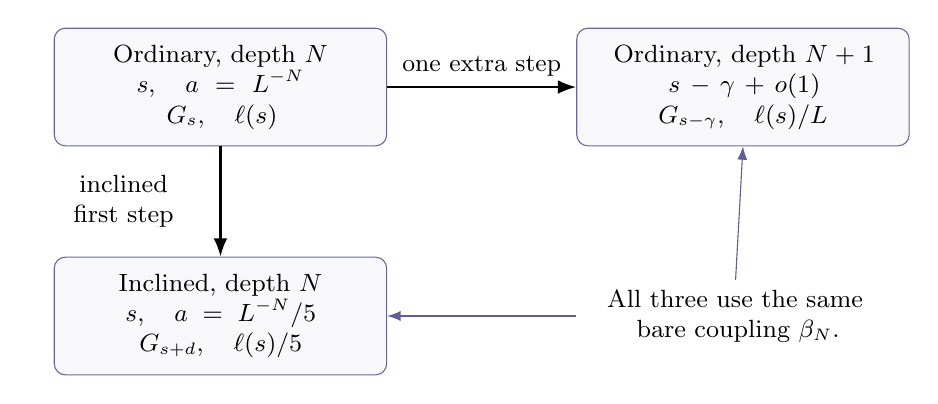
\begin{tikzpicture}[>=Latex,node distance=14mm and 24mm,
 every node/.style={font=\small,align=center},
 box/.style={draw=MidnightBlue!65,rounded corners,fill=MidnightBlue!3,
             inner sep=6pt,text width=38mm}]
\node[box] (a) {Ordinary, depth $N$\\
 $s,\quad a=L^{-N}$\\$G_s,\quad\ell(s)$};
\node[box,right=of a] (b) {Ordinary, depth $N+1$\\
 $s-\gamma+o(1)$\\$G_{s-\gamma},\quad\ell(s)/L$};
\node[box,below=of a] (c) {Inclined, depth $N$\\
 $s,\quad a=L^{-N}/5$\\$G_{s+d},\quad\ell(s)/5$};
\node[right=of c,text width=38mm] (d) {All three use the same\\bare coupling $\beta_N$.};
\draw[->,thick] (a)--node[above] {one extra step} (b);
\draw[->,thick] (a)--node[left,text width=22mm] {inclined\\first step} (c);
\draw[->,MidnightBlue!70] (d.north)--(b.south);
\draw[->,MidnightBlue!70] (d.west)--(c.east);
\end{tikzpicture}
\caption{The two scale comparisons.  The displayed offsets in the boxes
are the bare offsets of the trajectories; the inclined hierarchy matches
the ordinary hierarchy at $s+d$.  Canonical normalization cancels their
different field multipliers.  The inclined comparison retains only the
Euclidean rotation, as in \eqref{eq:uni-incline}.}
\label{fig:two-scales}
\end{figure}

\subsection{An elementary uniqueness mechanism}

We isolate the topological part of the argument.  Its input consists only
of continuous distributions, positive lengths, and the relations just
proved.  In particular, it requires no monotonicity of the shooting map.

\begin{lemma}[Two scale relations force constancy]\label{lem:dense-periods}
Let $L>1$ be a power of two, let $\gamma>0$, and let
$I=(-R,R)$.  Suppose $\ell:I\to(0,\infty)$ is continuous and
$s\mapsto G_s$ is a family of distribution hierarchies whose evaluation
on every Schwartz test is continuous.  Let $O_\pm$ be rotations by
$\pm\vartheta$, where $\cos\vartheta=3/5$ and
$\sin\vartheta=4/5$.  Suppose \eqref{eq:uni-depth} and
\eqref{eq:uni-incline} hold wherever both offsets belong to $I$, and
suppose $2R-|d|>\gamma$.
Then every $G_s$ is Euclidean rotation invariant, and $G_s$ is independent
of $s$.
\end{lemma}

\begin{proof}
First take $s$ in the interval $J=I\cap(I-d)$.  Equality of the two
pushforwards in \eqref{eq:uni-incline} implies invariance of $G_s$
under rotation by $2\vartheta$.  The number $\vartheta/\pi$ is
irrational.  Indeed, if it were rational, $e^{i\vartheta}$ would be a
root of unity, making
$e^{i\vartheta}+e^{-i\vartheta}=6/5$ an algebraic integer.  A rational
algebraic integer is an integer, which $6/5$ is not.  Powers of this
rotation are consequently dense in $SO(2)$.  The action of rotations
on Schwartz tests is continuous, so every distribution in $G_s$ is
invariant under all Euclidean rotations.  Equation~\eqref{eq:uni-incline}
therefore gives $G_{s+d}=G_s$ on $J$.

To use these local relations globally, extend the two families to
$\R$.  For $x\in\R$, choose an integer $n$ with $x+n\gamma\in I$ and
set
\begin{equation}\label{eq:uni-extension}
 \widetilde G_x=G_{x+n\gamma},\qquad
 \widetilde\ell(x)=L^{-n}\ell(x+n\gamma).
\end{equation}
Such an $n$ exists because $|I|>\gamma$.  These definitions do not
depend on the choice: two representatives can be joined by consecutive
$\gamma$-steps staying in the interval $I$, and
\eqref{eq:uni-depth} applies at every step.  On overlapping translates
of $I$, the definitions agree; hence the extended families are continuous.
They satisfy
\[
 \widetilde G_{x+\gamma}=\widetilde G_x,
 \qquad \widetilde\ell(x+\gamma)=L\widetilde\ell(x).
\]
The interval $J$ has length $2R-|d|>\gamma$, so every class modulo
$\gamma$ has a representative in $J$.  Choosing that representative in
\eqref{eq:uni-extension} transports both the rotation invariance and
the $d$-relations to every $x\in\R$:
\begin{equation}\label{eq:uni-global-periods}
 \widetilde G_{x+d}=\widetilde G_x,
 \qquad \widetilde\ell(x+d)=5^{-1}\widetilde\ell(x).
\end{equation}

If $d/\gamma=p/q$ with integers $p$ and $q>0$, then iterating the
length relations gives
\[
 5^{-q}\widetilde\ell(x)
 =\widetilde\ell(x+qd)
 =\widetilde\ell(x+p\gamma)
 =L^p\widetilde\ell(x).
\]
Since $\widetilde\ell(x)>0$, this would imply $5^{-q}=L^p$,
contradicting unique prime factorization.  Thus $d/\gamma$ is irrational.
The subgroup $\Z\gamma+\Z d$ is dense in $\R$.  Each test evaluation
of $\widetilde G$ is continuous and has this subgroup as periods, and
is therefore constant.  Equality on every test proves equality of the
hierarchies.  Restriction to $I$ proves the claim.
\end{proof}

\subsection{Every bare coupling and the physical conclusions}

\begin{proof}[Proof of Theorem~\ref{thm:canonical}]
Finiteness and strict positivity of $\chi_\beta$ and $\xi_\beta$ for
sufficiently large $\beta$ follow from Lemma~\ref{lem:finite-beta}.
Proposition~\ref{prop:two-scales} supplies the hypotheses of
Lemma~\ref{lem:dense-periods}; our choice of $R$ in
Section~\ref{sec:trajectories} gives the required overlap.  Write $G$
for the common normalized hierarchy.

The reference values $\vartheta_N$ tend to infinity, and
$\vartheta_{N+1}-\vartheta_N\to\gamma>0$.  For every sufficiently large
$\beta$, choose $N=N(\beta)$ so that
\[
 \vartheta_N\le\beta<\vartheta_{N+1}.
\]
Then $N(\beta)\to\infty$, and the offsets
$s(\beta)=\beta-\vartheta_{N(\beta)}$ belong to the fixed compact interval
$[0,2\gamma]\subset I$.  Any sequence $\beta_k\to\infty$ has a
subsequence on which these offsets converge to some $s\in I$.
Propositions~\ref{prop:offset-limits} and~\ref{prop:normalization}
give, along that subsequence, convergence of the canonically normalized
fields to $G$, jointly in law and in every joint moment, and strong
convergence of each component Schwinger distribution in $\mathcal S'$.
Moreover,
\[
 L^{-N(\beta_k)}\xi_{\beta_k}\longrightarrow\ell(s)>0,
\]
so $\xi_{\beta_k}\to\infty$ along the same subsequence.

These conclusions hold for a subsequence of every sequence tending to
infinity, with the same limiting hierarchy.  If any asserted convergence
failed, a sequence staying outside a fixed neighborhood of the claimed
limit would have such a subsequence, a contradiction.  This proves the
full $\beta\to\infty$ assertions.  The same argument applies to a
neighborhood in the strong topology of $\mathcal S'$; it does not require
that topology to be metrizable.  The finite-list laws are consistent, and
their local exponential moments determine them from $G$.

Finally let $\phi^{\mathrm{sh}}$ be the hierarchy in
Theorem~\ref{thm:main}, obtained by fixing a terminal kinetic coupling.
Its auxiliary parameters need not equal those used for the offset
argument.  Lemma~\ref{lem:shooting-normalization} gives finite positive
susceptibility $m_{\mathrm{sh}}$ and second-moment length
$\ell_{\mathrm{sh}}$, and convergence of the corresponding cutoff
quantities.  Thus its normalization
\begin{equation}\label{eq:uni-shooting-identification}
 \phi^{\mathrm{can}}(f)
 =\frac{1}{\ell_{\mathrm{sh}}\sqrt{m_{\mathrm{sh}}}}
    \phi^{\mathrm{sh}}\bigl(f(\,\cdot\,/\ell_{\mathrm{sh}})\bigr)
\end{equation}
is the limit of the same microscopic fields $\Psi_{\beta_N}$ along its
shooting sequence.  Since $\beta_N\to\infty$, this hierarchy is $G$.
Proposition~\ref{prop:normalization} also proves uniqueness of the
positive length and field constants fixing susceptibility and
second-moment length to one.
\end{proof}

\begin{proof}[Proof of Corollary~\ref{cor:canonical-physics}]
Equation~\eqref{eq:uni-shooting-identification} is a positive dilation
of space-time and multiplication of the field by a nonzero constant.
It preserves the Euclidean and internal symmetries, reflection
positivity, symmetry of the Schwinger functions, clustering, and their
factorial distributional bounds.  The reconstruction argument of
Section~\ref{sec:os} therefore applies.

More explicitly, substitution of the rescaled tests and field factors
defines an invertible map of the positive-time polynomial algebras and
preserves their Osterwalder--Schrader inner products.  It induces a
unitary map between the completed reconstructed spaces, taking vacuum
to vacuum.  A time translation by $t$ in canonical coordinates
corresponds to one by $\ell_{\mathrm{sh}}t$ in shooting coordinates.
Consequently the two Hamiltonians satisfy, under this unitary map,
\[
 H_{\mathrm{can}}=\ell_{\mathrm{sh}}H_{\mathrm{phys}}.
\]
The unique vacuum, the nonzero vacuum complement, and the positive
lower bound on the full vacuum-orthogonal Hamiltonian therefore persist.
A connected fourth distribution transforms by the nonzero fourth power
of the field factor and the invertible dilation of its tests.  Strict
separation of time supports is preserved by a positive dilation.
The nonzero separated connected fourth correlation of
Theorem~\ref{thm:main} thus remains nonzero in canonical units.
\end{proof}

\FloatBarrier
\bibliographystyle{plain}
\bibliography{references}
\end{document}
